\begin{filecontents*}{\jobname.xmpdata}
	\Title{Teaching Robots Social Autonomy From In Situ Human Supervision}
	\Author{Emmanuel Senft}
	\Keywords{Human-Robot Interaction\sep Interactive Machine Learning\sep Cognitive Robotics\sep Progressive Autonomy}
\end{filecontents*}

\documentclass[11pt, a4paper, twoside]{uopthesis}

\usepackage[top=20mm, bottom=20mm, inner=40mm, outer=24mm]{geometry}
\usepackage{graphicx,nomencl, natbib, microtype, titlesec, pdfpages, mathptmx, bibentry, booktabs, pdflscape, afterpage, framed, tabulary,subcaption,capt-of}
\usepackage{lettrine,paralist,fancyhdr}
\PassOptionsToPackage{hyphens,obeyspaces,spaces}{url}
\usepackage[colorlinks=false, breaklinks=true, hidelinks]{hyperref}
\usepackage{tabularx}
\newcolumntype{Y}{>{\centering\arraybackslash}X}
\usepackage[doublespacing]{setspace}		% double line spacing throughout
\usepackage[toc,page]{appendix}
\usepackage[ruled,vlined]{algorithm2e}
\usepackage{booktabs}
\newcommand{\ra}[1]{\renewcommand{\arraystretch}{#1}}
\nobibliography*
\graphicspath{{images/}}

\usepackage[markup=underlined]{changes}

\definechangesauthor[color=orange]{ES}
\newcommand{\ES}[1]{\added[id=ES]{#1}}
\newcommand{\ESc}[2]{\added[id=ES,remark={#1}]{#2}}
\newcommand{\ESd}[1]{\deleted[id=ES]{#1}}
\newcommand{\ESr}[2]{\replaced[id=ES]{#2}{#1}}

\makeatletter
\g@addto@macro{\UrlBreaks}{\UrlOrds\do\r}
\makeatother

\makeatletter
\newcommand{\thickhline}{%
	\noalign {\ifnum 0=`}\fi \hrule height 1pt
	\futurelet \reserved@a \@xhline
}
\newcolumntype{"}{@{\hskip\tabcolsep\vrule width 1pt\hskip\tabcolsep}}
\makeatother

\usepackage[acronym,toc]{glossaries} 
\makeglossaries

\newacronym{ml}{ML}{Machine Learning}
\newacronym{lfd}{LfD}{Learning from Demonstration}
\newacronym{iml}{IML}{Interactive Machine Learning}
\newacronym{cml}{CML}{Classical Machine Learning}
\newacronym{sar}{SAR}{Socially Assistive Robotics}
\newacronym{rat}{RAT}{Robot Assisted Therapy}
\newacronym{rl}{RL}{Reinforcement Learning}
\newacronym{sl}{SL}{Supervised Learning}
\newacronym{asd}{ASD}{Autism Spetrum Disorder}
\newacronym{chri}{cHRI}{Child-Robot Interaction} 
\newacronym{hri}{HRI}{Human-Robot Interaction}
\newacronym{hhi}{HHI}{Human-Human Interaction}
\newacronym{hci}{HCI}{Human-Computer Interaction}
\newacronym{ci}{CI}{Confidence Interval}
\newacronym{dream}{DREAM}{Development of Robot-Enhanced Therapy for Children with Autism Spectrum Disorders (European FP7 project)}
\newacronym{woz}{WoZ}{Wizard-of-Oz}
\newacronym{sparc}{SPARC}{Supervided Progressive Autonomous Robot Competenties}


\titleformat{\chapter}[display]
  {\normalfont\huge\bfseries}{\chaptertitlename\ \thechapter}{20pt}{}

% make all page numbers in the right place and remove heading line
%\pagestyle{fancy}
%\lhead{}
%\chead{}
%\rhead{}
%\lfoot{}
%\cfoot{\thepage}
%\rfoot{}
%\renewcommand{\headrulewidth}{0pt}

% --- for more modern look - take these out for old fashioned look to the paragraphs
\parindent=0pt
\parskip = 6pt

%\usepackage{uarial}
%\usepackage{tgheros}
%\usepackage{helvet}
%\usepackage{charter}
%\usepackage{garamond}
%\usepackage{MyriadPro}
%\usepackage{mathpazo}
%\usepackage{eulervm}
%\usepackage{venturis2}
%\renewcommand{\familydefault}{\sfdefault}
\usepackage[T1]{fontenc}
\renewcommand*\familydefault{\sfdefault}
\usepackage[scaled=1]{helvet}
%\usepackage[helvet]{sfmath}
%\everymath={\sf}

\newcommand\cleartooddpage{\clearpage
  \ifodd\value{page}\else\null\clearpage\fi}

\usepackage{mathptmx}

% --- nice typewriter alternative
\usepackage{tgcursor}

%%%%%%%%%%%%%%%%%%%%%%%%%%%%%%%%%%%%%%%%%%%%%%%%%%%%%%%%%%%%%%%%%%%%%%%%%%%%
\begin{document}

\onehalfspacing
%%%%%%%%%%%%%%%%%%%%%%%%%%%%%%%%%%%%%%%%%%%%%%%%%%%%%%%%%%%%%%%%%%%%%%%%%%%%
% --- the title and copyright are not chapters so needs a cleardouble page after
\pagenumbering{gobble}
This copy of the thesis has been supplied on condition that anyone who consults it is understood to recognise that its copyright rests with its author and that no quotation from the thesis and no information derived from it may be published without the author's prior consent.

\cleartooddpage

%%%%%%%%%%%%%%%%%%%%%%%%%%%%%%%%%%%%%%%%%%%%%%%%%%%%%%%%%%%%%%%%%%%%%%%%%%%%
% --- this is the line that puts the title page in from the pdf file
\begin{center}
\begin{figure}[h]
\centering

\includegraphics[width=0.5\linewidth]{newCrest.jpg}
\end{figure}
\vspace{36pt}
\LARGE 
\textbf{Teaching Robots Social Autonomy From In Situ Human Supervision}
\\
\vspace{12pt}
\Large by
\\
\vspace{12pt}
\LARGE 
Emmanuel Senft
\\
\vspace{48pt}
\Large 
A thesis submitted to the University of Plymouth
\\
in partial fulfilment for the degree of
\vspace{36pt}
\\
\textbf{DOCTOR OF PHILOSOPHY}
\vspace{36pt}
\\
School of Computing, Electronics and Mathematics\\
Faculty of Science and Engineering
\vspace{36pt}
\\
%\textit{In collaboration with \\ Rutland Port Authorities}
\vspace{36pt}
%\\
November 2018
\end{center}

% --- make sure you switch the size selection back to normal
\normalsize

\cleardoublepage

\chapter*{Acknowledgements}	
\addcontentsline{toc}{chapter}{Acknowledgements}
Thanks Séverin, Paul and of course Tony

  

\chapter*{Author's declaration}
\addcontentsline{toc}{chapter}{Author's declaration}
At no time during the registration for the degree of Doctor of Philosophy has
the author been registered for any other University award. Work submitted for
this research degree at Plymouth University has not formed part of any other
degree either at Plymouth University or at another establishment.

This work has been carried out by Emmmanuel Senft under the supervision of Prof.
Dr. Tony Belpaeme, Dr. Paul Baxter, and Dr. S\'{e}verin Lemaignan. The work was
funded by European Union FP7 projects DREAM (grant no.: 611391).

\subsection*{Parts of this thesis have been published by the author:}

\bibentry{senft2015human}

\bibentry{senft2015sparc}

\bibentry{senft2015better}

\bibentry{senft2016providing}

\bibentry{senft2016sparc}

\bibentry{senft2017supervised}

\bibentry{senft2017toward}

\bibentry{senft2017leveraging}

\bibentry{senft2018robots}

\subsection*{Collaborative work published but not included in this research:}

\bibentry{kennedy2015higher}

\bibentry{baxter2015touchscreen}

\bibentry{kennedy2015using}

\bibentry{baxter2015wider}

\bibentry{kennedy2016social}

\bibentry{baxter2016characterising}

\bibentry{kennedy2016heart}

\bibentry{wills2016socially}

\bibentry{kennedy2017child}

\bibentry{esteban2017build}

\bibentry{lara2017human}

\bibentry{lemaignan2017free}

\bibentry{irfan2018social}

\bibentry{cao2018personalized}

\bibentry{casas2018social}

%Talks at conferences and workshops:
%\begin{itemize}
%	\item MLIS
%	\item ICSR
%	\item R4L HRI
%	\item Off the lips
%\end{itemize}

\vspace{1.0cm}

Word count for the main body of this thesis:~\textbf{}

% --- signature block
\vspace{1.0cm}

\makebox[2cm][l]{\textbf{Signed:}}\rule{0.4\textwidth}{0.3pt}

\vspace{1cm} 

\makebox[2cm][l]{\textbf{Date:}}\rule{0.4\textwidth}{0.3pt}

\cleardoublepage

\chapter*{Abstract}	
\addcontentsline{toc}{chapter}{Abstract}
\textbf{TEACHING ROBOTS SOCIAL AUTONOMY FROM IN-SITU HUMAN SUPERVISION}\newline
\textbf{Emmanuel Senft}

To reach the potential promised to robots in interaction with humans, robots need to learn from them. Knowledge of expected robot behaviours does not lie in engineers' hand but in the end-users'. As a consequence, to reach new applications and enter daily lives, robot users need to be provided with a way to teach their robot to interact in the way they desire.

The thesis explored by this work is that a robot can learn to interact meaningfully with humans in an efficient and safe way by receiving supervision from a human teacher in control of the robot's behaviour. This work original contribution to knowledge is a new teaching framework applicable to robotics and addressing the thesis: the \gls{sparc} and its evaluation in three studies. \gls{sparc} aims at enabling non-technical users to teach a robot in high stakes environments such as \gls{hri}. By providing the teacher with control over the robot, \gls{sparc} ensures that every action executed by the robot has been actively or passively approved by the teacher. This approach demonstrated its applicability to \gls{hri} by successfully teaching a robot to tutor children in an educational game, resulting similar behaviours for the autonomous robot and the one controlled by a human.

Throughout evaluating \gls{sparc}, this work contributes to extend our knowledge on how humans teach autonomous agents and the impacts of the teacher-robot interface's features on the teaching process. It is found here that a supervised robot learning from a human could reduce the workload required to express a useful robot behaviour. Furthermore, providing the teacher with the opportunity to control the robot's behaviour improves substantially the teaching process and can lead to an autonomous robot interacting efficiently with humans.

\ES{reopening?}



%This work original contribution to knowledge is a new teaching paradigm for robotics: \gls{sparc} which has been validated in three studies: interaction with a model, interaction with a fixed environment and interaction with humans in the context of robotic tutors.

%First? demonstration of teaching a robot online to interact with humans  

\tableofcontents
\listoffigures
\cleartooddpage

\setcounter{page}{1} 
\renewcommand{\thepage}{\arabic{page}}			
\pagestyle{fancy}


\newcommand{\thesis}{Through receiving supervision from a human teacher, a robot can progressively and efficiently learn a policy for interacting with people, during the learning the robot will at all times display correct behaviour}

\doublespacing
%%%%%%%%%%%%%%%%%%%%%%%%%%%%%%%%%%%%%%%%%%%%%%%%%%%%%%%%%%%%%%%%%%%%%%%%%%%%
%%%%%%%%%%%%%%%%%%%%%%%%%%%%%%%%%%%%%%%%%%%%%%%%%%%%%
\chapter{Introduction} \label{chap:intro}
\graphicspath{{images/intro/}}

\gls{hri} what it is and what it matters and why it is challenging

Robots will inhabit human spaces and need to interact with them in decent ways

Robot behaviour unlikely to be programmable and static

This works explores how robots could interact with humans to learn from them to interact with other humans

%%%%%%%%%%%%%%%%%%%%%%%%%%%%%%%%%%%%%%%%%%%%%%%%%%%%%
\section{Scope}\label{sec:intro-scope}

Enabling a robot to interact socially with humans is complex task. The robot needs to interpret a large sensory space, relying on images camera, motor joints or high level concepts defining the state of the interaction. Then based on the interpretation of this inputs and rules defining expected behaviour or limiting the behaviour, the robot needs to select an action or a plan it will execute to fit the goal it has been assigned. The following sections will aim to refine the scope of the research conducted in this thesis.

\subsection{Frame}

The focus of the research conducted here is finding a way for robots to interact safely and efficiently with humans. It has been argued by many \citep{dautenhahn2004robots,billard2008robot} that an efficient robot interacting with human would not be preprogrammed beforehand and execute a one-size-fits-all policy suited to every possible interaction partners. Robots needs to be able to learn an interactive behaviour, improving their skills as they interact and personalising their policy to the preferences of their users. The aim of this thesis is finding a interaction framework allowing humans to teach robot how to interact with other humans.  

Throughout this thesis we make the assumption that, while an engineer designing a robot behaviour might not know how the robot should behave, an expert possess this knowledge and should be able to transfer it to the robot. This human teacher's expertise is not related to theoretical knowledge in \gls{ml}, robotics or other scientific fields. It just denotes that this person possess knowledge unknown by the engineer design the robot. This could take the form of the steps of a therapy a robot should deliver to the child (known by a therapist) or more simply a senior's preferences and desires concerning a robot companion.

This thesis aims to provide a convenient and efficient way for this domain expert to inculcate this knowledge in the robot.


\subsection{Environment} 

Robots considered in this thesis evolve in human-centred environment and are expected to provide some support to the surrounding humans and achieve a specific goal assigned to them. Interactions with humans are by essence social, and robots needs to take into these social norms when interacting in human environments.

???

\subsection{Type of Interaction}

The typical interaction considered in this thesis is a triadic interaction between a human the user of the robot, the robot and an application target, potentially another human (as shown in Figure \ref{fig:intro_setup}). In this type of interaction, the user has an aim for robot, a task they would like the robot to complete. And through the teaching interaction, they can supervise the robot, demonstrating it what it should do and teaching it an efficient action policy in the application interaction with the target.

The application target could be another human (such as a child receiving teaching support from the robot) or just parts of the environment if the robot has to complete a manipulation of navigation task (such as picking up a book in the library).

\begin{figure}[ht]
	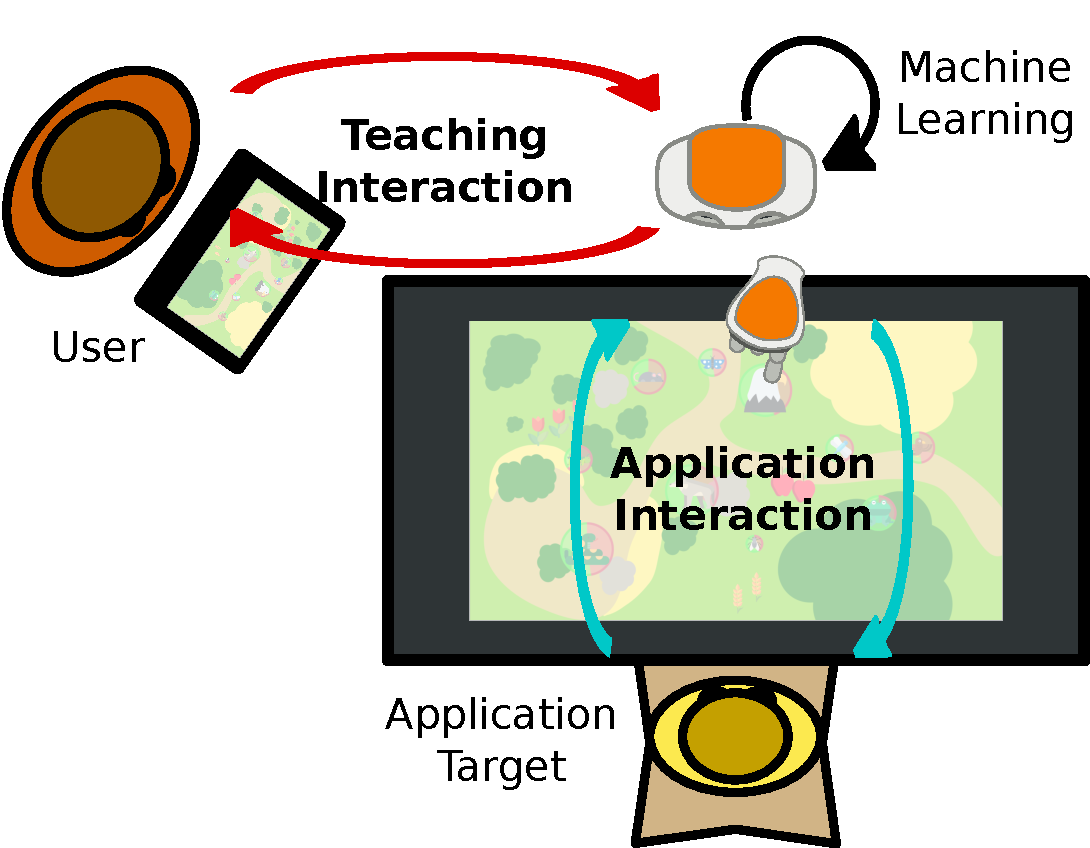
\includegraphics[width=.7\linewidth]{setup.pdf}
	\centering
	\caption{The typical interaction used in this research: a robot interacts with a target in an application interaction and learns from a domain expert through a teaching interaction.}
	\label{fig:intro_setup}
\end{figure}

\subsection{Algorithms}

The aim of this thesis being exploring how humans could teach robots to interact in  human-centred environment, the robot needs to possess a learning algorithm allowing it to improve its action policy. Two main categories of learning algorithms have been used in this research: \gls{sl} and \gls{rl}.

\gls{sl} aims to learn a mapping between inputs and outputs to automatically reproduce a desired behaviour. It uses a dataset of labelled example and optimise an algorithm such as its prediction error of the output for each input is minimised \citep{russell2016artificial}. Typical example used in this study are \gls{ann} and nearest neighbours methods. \gls{ann} models loosely the way brains and neurons work by having a group of `neurons' connected between each other by synapses. Each neuron updates its according value according to connections with other neurons including weights and non-linearity. The general approach have a set of input nodes, a set of output nodes and hidden nodes, and the network learns by changing the value of the weights to reproduce the desired values on the output nodes. Nearest neighbours methods compare the distance in the feature space between a point to classify to the different instances stored in a dataset and select the value of a majority of nearest neighbours in this space.

Unlike \gls{sl} which aims at reproducing a known behaviours, \gls{rl} aims at providing an agent with the capacity to discover the world it interact in and learn from this interaction with the world \citep{sutton1998reinforcement}. The agent has access to a description of the state and actions it can do, and depending of the action selected, the state will change and the agent will receive a reward. The goal of the agent is to find an optimal policy maximising a notion of cumulated reward.

Due to the relevance of both fields to this thesis research topics: enabling humans to teach robots to interact, algorithm from both categories have been used. The first study presented in Chapter \ref{chap:woz} uses a feed forward neural network learning to reproduce a teacher policy. The second study in Chapter \ref{chap:control} used \acrlong{rl} combining human and environmental rewards. The aim of this algorithm is to use the human guidance and rewards to learn an efficient interaction policy. And the last study presented in Chapter \ref{chap:tutoring} uses instance based algorithm adapted from Nearest Neighbours to enable quick and efficient learning. More details about each algorithms and their related work can be found in the associated chapters.

%%%%%%%%%%%%%%%%%%%%%%%%%%%%%%%%%%%%%%%%%%%%%%%%%%%%%
\section{The Thesis}\label{sec:intro-thesis}
The main thesis that this document seeks to put forward is as below.
\begin{quote}
	A robot can learn how to interact meaningfully with humans by receiving supervision from a human teacher in control of the robot's behaviour, this supervision will lead to an efficient, safe and low human-workload teaching and autonomous behaviour.	
\end{quote}
%One sentence to describe the take home/conclusion

Additional research questions have been explored during the progress of this
work and are introduced here.

\begin{itemize}
    \item \textbf{What kind of interaction could allow a human to teach a robot to interact with other humans while ensuring an appropriate and adaptive interaction policy and a low workload on the human teacher?}
    
    	Justification for \gls{sparc} 
    \item \textbf{Does adding a learning component to a supervised robot can reduce the human-workload of the supervisor?}
    
        \gls{woz} is an approach widely used in \gls{hri} \citep{riek2012wizard}, whereby a human teleoperates a robot to have it interact with other humans. However, this method applies a high workload on the operator and is not scalable. Using \gls{ml} to learn from this operator online might decrease the operator's workload without decreasing the quality of the robot behaviour.
    
    \item \textbf{How control of a teacher over the robot's action impacts the robot's learning?} 
    
	    In the context of \gls{iml}, a human can provide inputs to an agent to speed up the learning. Other \gls{iml} \citep{thomaz2008teachable,knox2009interactively} focus on feedback from the human with limited or no control over the agent's actions. However increase the control should speed up the learning and reduce the number of errors made by the robot.

    \item \textbf{After receiving supervision from a human, could a robot behave autonomously in a social context?}

	 	\gls{sparc} has been designed to allow non-experts in \gls{ml} to teach agents how to interact while interacting. Human-robot interactions provide a perfect test for this approach: using a human to teach a robot how to behave in this complex and non-deterministic environment.
	 
\end{itemize}

%%%%%%%%%%%%%%%%%%%%%%%%%%%%%%%%%%%%%%%%%%%%%%%%%%%%%
\section{Approach and Experimentation}\label{sec:intro-exps}
%Should make more references to the research questions
To explore the thesis and research questions addressed in this work, in Chapter \ref{chap:background}, we started by reviewing the fields of application of \gls{hri} where the interaction is social. From this review, we drew requirements a robot controller should follow. Then we analysed the different controllers used in robotics through these requirements and identified the absence of controller used in \gls{hri} validating this principles.

To address this lack of method providing appropriateness of actions and adaptivity to robots while requiring a low workload, we proposed a new method, \gls{sparc}, applicable to \gls{hri}. \gls{sparc} aims to provide control over the robot's action to a human and use this supervision to learn online a correct action policy. \gls{sparc} is based on principles allowing this interaction to be efficient... Once the method and the principles defining the interaction between the human teacher and the robot defined, we evaluated this approach in three study with increasing ambition. Before testing \gls{sparc} in a real world interaction, we needed to evaluate if the interaction between the teacher and the robot could lead to a learning of the robot side, a decrease of workload on the teacher side and if the control provided by \gls{sparc} improved the safety and the efficiency of the learning process.

The first study, presented in Chapter \ref{chap:woz}, aims at evaluating the interaction between the supervisor and the robot in a controlled and repeatable environment inspired by \gls{rat}. The study explores how, by decreasing the number of actions required by the supervisor, the learning component of \gls{sparc} can reduce their workload.

Once \gls{sparc} demonstrated that it allowed a robot to learn and decreased the workload on the supervisor, we evaluated how the control provided by \gls{sparc} improved the learning process. To explore the impact of control, we designed a second study comparing \gls{sparc} to \gls{irl} an alternative approach used to teach robots, but providing less control over the robot's action to the teacher. Similarly to the first study, this second one only included a human as a teacher, but not in the target of the teaching. This allowed to gather information on \gls{sparc} in repeatable environments and without having to tackle the challenges of interacting in the real world.

Since the two first study demonstrated the efficiency of \gls{sparc} to teach a robot to interact in virtual environments, \gls{sparc} was ready to be evaluated in a real human-robot interaction: tutoring children in the wild. This last study applied \gls{sparc} to teach a robot a social policy to interact with humans and support child learning. And this study aims at demonstrating the applicability of \gls{sparc} in teaching robots to interact socially with humans, consequently supporting the thesis of this research.

ow the results have been used to design a new interaction framework to teach robots to interact with humans

how it has been tested and why that order

%%%%%%%%%%%%%%%%%%%%%%%%%%%%%%%%%%%%%%%%%%%%%%%%%%%%%
\section{Key Concepts and Terminology}\label{sec:intro-concepts}

Not sure if worth including

Throughout this thesis, the terms `wizard', `supervisor', `user', `expert' and `teacher' have been used interchangeably to represent the people in control of a robot's action and teaching that robot an action policy.

agent and robot

\begin{itemize}
	\item \textbf{Appropriateness}:
	\item \textbf{Adaptivity}
	\item \textbf{Autonomy}
	\item \textbf{Supervised Autonomy}
	\item \textbf{Learning}
	\item \textbf{Teacher, wizard, user, expert and supervisor}
	\item \textbf{Robot and agent}
\end{itemize}

%%%%%%%%%%%%%%%%%%%%%%%%%%%%%%%%%%%%%%%%%%%%%%%%%%%%%
\section{Challenges}

Complexity of interactions with humans: complex world, safety, workload and so on

%%%%%%%%%%%%%%%%%%%%%%%%%%%%%%%%%%%%%%%%%%%%%%%%%%%%%
\section{Contributions}\label{sec:intro-contr}

\subsection{Scientific Contribution}
\begin{itemize}
	\item Design of a new interaction framework for teaching agents in a safe way.
	\item Evaluation in three studies.
	\item Demonstration of the importance of control over the robot's action when teaching a robot to interact.
	\item Design of a lightweight algorithm to quickly learn from demonstration in complex environments.
	\item Application of \gls{iml} to safely teach robots social autonomy from in situ human supervision. 
\end{itemize}

\subsection{Technical Contribution}
\begin{itemize}
	\item Software development for two projects: \acrshort{dream} (European FP7 project: 611391) and Human-Robot Interaction Strategies for Rehabilitation based on Socially Assistive Robotics (Royal Academy of Engineering: IAPP\textbackslash1516\textbackslash137).
	\item Development of a Wizard interface for the Freeplay-Sandbox\footnote{\url{https://github.com/freeplay-sandbox}}. 
\end{itemize}
	
%%%%%%%%%%%%%%%%%%%%%%%%%%%%%%%%%%%%%%%%%%%%%%%%%%%%%
\section{Structure}\label{sec:intro-struct}
The structure of this thesis is outlined below to provide an overview of the content and context for each chapter. A summary of key experimental findings are included at the start of each relevant chapter for ease of reference. 

\begin{itemize}
	\item This chapter provided an introduction to the general field of this research (robots learning to interact with humans), the research questions including the central \textit{thesis}, scope, and contributions of the work presented in later chapters.  

	\item Chapter~\ref{chap:background} provides a description of the different fields of \gls{hri} and draws three requirements for robot's controllers interacting with humans. In a second part, it analyses the current controllers for robots in \gls{hri} identifying that no current controller fits these requirements. Finally, it proposes to apply \gls{iml} to \gls{hri} to validate the requirements, which is the goal of this thesis.
	
	\item Chapter~\ref{chap:sparc} proposes a new interaction framework, \gls{sparc}, aiming to provide a way to apply \gls{iml} to \gls{hri} while validating the three requirements proposed in Chapter \ref{chap:background}. Additionally, this chapter presents the expectations of \gls{sparc}.
	
	\item Chapter~\ref{chap:woz} presents results from a first study evaluating if the principles of \gls{sparc} would allow to reduce the workload on a supervisor compared to \gls{woz}. Results support the hypotheses, validating some of the motivation of \gls{sparc} (a learning robot would reduce the workload on a supervisor).
	
	\item Chapter~\ref{chap:control} presents results from a second study comparing \gls{sparc} to \gls{irl}, another interaction framework from \gls{iml}. The main difference between the two approaches is the amount of control the teacher has. With \gls{sparc}, the teacher can correct any action executed by the robot, and results support that this control improves the efficiency of the learning (performance, time and inputs required to teach and risks taken during the teaching phase).
	
	\item Chapter~\ref{chap:tutoring} presents a study where \gls{sparc} has been applied to a real world \gls{hri}, child tutoring. And results demonstrate that while not impacting the learning gain of the session, an autonomous robot having learned using \gls{sparc} elicit similar children behaviour than a supervised robot, unlike a passive robot. This results support \gls{sparc} as a teaching method allowing to transfer a social and technical action policy from human expert to a robot in a safe way.
	
	\item Chapter~\ref{chap:discussion} presents a discussion from the main findings from the previous chapters and presents limitations and future directions of research for \gls{sparc}.
	
	\item Chapter~\ref{chap:conclusion} concludes the thesis and presents a summary of the main contributions.
	
\end{itemize}

\cleartooddpage

%%%%%%%%%%%%%%%%%%%%%%%%%%%%%%%%%%%%%%%%%%%%%%%%%%%%%
\chapter{Background} \label{chap:background}
\glsresetall

This chapter describes social \gls{hri} and presents related research in agent and robot control. The first section introduces the different fields of application of social \gls{hri} and draws from them requirements for controlling a robot interacting with humans (the robot should: only execute appropriate actions and have a high level of adaptivity and autonomy). The second section provides the current state of the art in robot control for \gls{hri} and analyses it through the requirements presented in the previous section. And finally, building on the lack of controller satisfying the requirements from Section 1, the third section presents \gls{iml}, an alternative method holding promises to teach agents how to interact and how it could be applied to \gls{hri}.

\section{Social Human-Robot Interaction}

\subsection{Fields of Application} \label{ssec:back_hri}

Reviews of \gls{hri} and socially interactive robots have already been presented in \cite{fong2003survey}, \cite{goodrich2007human} and \cite{sheridan2016human}. However, these reviews are starting to be dated and/or did not have the same focus than this research. As mentioned in the introduction, this work is focused on social robots, robots perceived as social agents and interacting in a human-centred environment. Depending of the context of interaction, these social robots will have been designed to interact socially with humans, or sometimes, the perception of sociality and agency will simply emerge from the interaction~\citep{fincannon2004evidence}. As such, the following criteria on the interactions were used to select the subfields of \gls{hri} relevant to this research:
\begin{itemize}
	\item Presence of an interaction between a robot and a human: both the human and the robot are influencing each other's behaviour.
	\item The human partner considers the robot as a social agent, responding socially to the robot and potentially bonding with it.
\end{itemize}

We reorganised and edited Goodrich and Schultz's categories, to fit with the criteria presented above, which resulted in five subfields involving social interactions between robots and humans: 
\begin{itemize}
	\item \acrfull{sar}
	\item Education
	\item Search and Rescue, and Military
	\item Hospitality, Home and Entertainment
	\item Collaborative Robots in Industry
\end{itemize}
We updated each category with recent research and highlighted the social component of the interaction and its impact on the controller used for the robot.

\subsubsection{Socially Assistive Robotics}

	\gls{sar} is a term coined by \cite{feil2005defining} and refers to a robot providing assistance to human users through social interaction. This field has been defined by \cite{tapus2007socially} as one of the grand challenges of robotics.
	
	One of the main applications of \gls{sar} is care for the elderly. In the near future, the ageing of population will have large impacts on the world, and societies will have to find solutions to tackle this challenge. The \cite{united2017world} reports that the ``population aged 60 or over is growing faster than all younger age groups''. This unbalance of growth will decrease the support ratio (number of workers per retiree) forcing societies to find ways to provide care to an increasing number of people using a decreasing staff. Robots represent a unique opportunity to compensate for this lacking workforce potentially allowing elderly to stay at home rather than joining elderly care centres~\citep{di2014web} or simply to support the nursing staff~\citep{wada2004effects}.
	
	%For this reason, robots for the elderlies is one of the major robotic market today and for the next decades as demonstrated by the number of projects all around the globe targeting this issue: Robot-Era~\citep{bevilacqua2012robot}, Accompany project~\citep{amirabdollahian2013accompany}, CompanionAble~\citep{badii2009companionable}  and the Robear project in Japan    \footnote{\url{http://www.riken.jp/en/pr/press/2015/20150223_2/}} to cite     only a small subset of them.	
	
	%Might want to remove
    %However, the acceptance of these robots in elderly care facilities or at their homes may still be problematic. Multiple studies report a good acceptance of robot and positive effects on stress in home cares both for the elderly and the nursing staff~\citep{wada2004effects,tamura2004entertainment}. But as mentioned by \citet{broadbent2009acceptance}, this acceptance could be increased by matching more closely the behaviours of the robots to the actual patients' needs and expectations.
		
	The second main application of \gls{sar} is \gls{rat}. Robots might be used to provide therapies or to follow and support a patient during their rehabilitation to improve their health, their acceptance in society or recover better from an accident. In therapies, robots were first used as physical platforms to help patient in rehabilitation therapy during the 80s~\citep{harwin1988robot}. During this period, robots were primally used as mechatronic tools helping humans to accomplish repetitive task. But in the late 90s, robots started to be used for their social capabilities. For example the AuRoRA Project~\citep{dautenhahn1999robots} started in 1998 to explore the use of robots as therapeutic tools for children with \gls{asd}. Since AuRoRA, many other projects, such as the DREAM project\footnote{\url{https://www.dream2020.eu}}, have started all around the world to use robots to help patient with ASD~\citep{diehl2012clinical,esteban2017build}. 
	
	\gls{rat} is not limited to \gls{asd} only, this use of robots is also explored in hospitals, for example to support children with diabetes~\citep{belpaeme2012multimodal}, to support elderly with dementia~\citep{wada2005psychological} and stroke recovering patients~\citep{mataric2007socially} or to monitor and provide encouragement in cardiac rehabilitation therapies~\citep{lara2017human}.	
	
	These examples demonstrate that already today, robots are interacting with vulnerable populations (children, the elderly or patients in therapy). This implies that robots' social behaviours need to be constantly correct to ensure that no harm will be caused to these populations. And due to the shortage of workforce, these robots also need to be as autonomous as possible.
	
\subsubsection{Education} 
	Social robots are being used in education, supporting teachers to provide learning content to children and transforming the teaching process from passive learning to active learning~\citep{linder2001facilitating}. In education, robots can take multiple roles such as peer, tutor or tool~\citep{mubin2013review}. It should be noted that Mubin et al. stress that the intention of the robotic community is not to replace teachers by robots, but provide them with a new form of technological teaching aid. Nevertheless, \cite{verner2016science} presented positive results from an early stage study using a tall humanoid robot to deliver a science lesson to children. The remaining of the section will describe more in details the roles of tutor and peer robots (the `tool' role has been excluded due its general lack of perceived gency and the lack social interaction between the robot and the students).
	
	\paragraph{Robotics tutors providing tailored teaching content in 1 to 1 interaction.} 
	Individualised feedback has been shown to increase the performance of students~\citep{cohen1982educational,bloom19842}. However, tutoring requires a larger trained staff and as such is more costly than large classes supervised by a single teacher. For this reason, tutoring is seldom used in public education today. Tutoring is however often available through private teacher at additional cost for the parents, potentially increasing social inequalities~\citep{bray2009confronting}. Robotic tutors could provide this powerful one to one tailored interaction to every student during school time, leading to higher learning gain for the children without dramatically increasing the workload on teachers or the price of education ~\citep{kanda2004interactive,leyzberg2012physical,kennedy2016social,gordon2016affective}. In addition to classroom uses, robots could also support children at home as they have been shown to elicit advantages over web or paper based instructions~\citep{han2005educational}. 
	
	\paragraph{Peer robots learning alongside the children.}
	Unlike other types of agents in education, peer robots have the opportunity to fit a special role seldom present in education today: the role of care-receiver rather than care-giver~\citep{tanaka2012children}. Peer learning has demonstrated benefits both for the helpers and those helped in \gls{hhi}~\citep{topping2005trends}. In \gls{hri}, a peer robot does not mentor a child to teach them new concepts, but learns alongside or from them, supporting them during the process and encouraging these children to produce behaviours improving their own learning. For example, in the Co-Writer project~\citep{hood2015children}, a child has to teach a robot how to write, and as the child demonstrates correct handwriting to the robot, they improve their own skills at drawing letters. Peer robots are able to leverage the concept of learning by teaching~\citep{frager1970learning} and peer learning~\citep{topping2005trends} in a way hardly matched by humans. The robot can take the role of a less knowledgeable agent with endless patience and encourage the student to perform repetitive tasks such as handwriting. In a similar position, an adult would not be a believable agent requiring learning and a younger student might not have the compliance and the patience to learn from another child.
	
	To provide efficient tutoring or peer support, robots need to be able to personalise their behaviour to the children they are interacting with in order to maximise the children's learning gain. Additionally, as pointed by \citet{kennedy2015robot}, a robot too social could decrease the children's learning compared to a less social robot if its behaviour is not congruent, consequently the robot's social behaviours have to be carefully managed to ensure its effectiveness. 
	
\subsubsection{Search and Rescue, and Military} 
	%\ES{have a look to goodrich}
    Robots are already deployed in the real world, outside of labs and used during search and rescue missions~\citep{casper2003human,murphy2004human}. For instance, after a natural or artificial catastrophe, robots have been sent to analyse the damaged area and report or rescue the surviving victims of the incident. During these missions, robots have to interact socially with two kinds of human partners: the survivors and the rescue team. In both cases the social component of the interaction is key. The survivor is probably in a shocked state and the searching robot could be the first link they have with the external world after the accident~\citep{murphy2008search}. In this case, a social response is expected from the robot and it has to be carefully controlled. On the other side, the rescue team monitoring the robots is under high pressure to act quickly and faces traumatic events too. Even if the robot does not display a social behaviour, rescuers interacting with it might develop some feeling toward the robots they are using during these tense moments~\citep{fincannon2004evidence}.
	
    Similar human behaviours (i.e. emotional bonding with a teleoperated robot) have also been observed in the army~\citep{singer2009wired}. Robots have been deployed as teleoperated drones and ground units alongside soldiers to complete scouting task or cleaning minefields. By interacting with a robot for extensive periods, some soldiers developed feelings toward this robot they used in a daily basis: taking pictures with it and introducing it to their friends. These relationships have gone as far as soldiers risking their own life to in order to save the robot used by their squad~\citep{singer2009wired}. 
    
    These examples in these two fields demonstrate that even in interactions where the robot is not supposed to interact socially with humans, its users might consider it as a social agent. Consequently, the sociability of the robot has to be taken into account when interacting in such stressful environments. Overlooking the importance of social relationships human will form can lead to dramatic consequences (e.g. soldiers taking risks for the robot). As such, during the interaction, the robot's behaviour needs to be constantly appropriate not to create misleading expectations and to ensure that the goal of the interaction will be met.
		
\subsubsection{Hospitality, Home and Entertainment} 
	
	Robots are also interacting with humans in hotels around the world; for example, the Relay robot (Savioke\footnote{\url{http://www.savioke.com/}}) delivers amenities directly to the guests' rooms in more than 70 hotels in the US, Europe and Japan\footnote{\url{https://www.spectrum.ieee.org/view-from-the-valley/robotics/industrial-robots/ces-2018-delivery-robots-are-fulltime-employees-at-a-las-vegas-hotel}}. Whilst the social interaction is still minimal today, these robots interact everyday with humans and have been seen evoking social reactions from them\footnote{\url{https://www.fastcodesign.com/3057075/how-savioke-labs-built-a-robot-personality-in-5-days}}. 
	
	Since the late 90s, scientists explored how robots could guide visitors in museums and exhibitions~\citep{thrun1999minerva,burgard1999experiences}. These researches continue today to explore how to improve the social interaction between tourists and these guide robots~\citep{bennewitz2005towards}. In a similar context, researchers have designed and tested a robot as a receptionist in a hall at Carnegie Melon University~\citep{gockley2005designing}. Studies have also explored long term interactions and how humans perceive and interact with robots in shops and shopping malls~\citep{kanda2009affective} and how robots should behave with clients~\citep{kanda2008will}.

    Finally, robots have already entered homes and family circles: from vacuum cleaners to companion passing by pet robots. A notable example is Aibo: twenty years ago, Sony created Aibo, a robotic dog to be used as pet in Japanese families and a new version was released in early 2018\footnote{\url{https://aibo.sony.jp/en/}}. An analysis of online discussions of owners published 6 years after Aibo's first introduction gives insights on the relationship that owners created with their robots~\citep{friedman2003hardware}. For example 42\% of the community members assigned intentionality to the robot, such as preferences, emotions or even feelings. Similar behaviours have also been observed when the robot was used not as a pet, but even just as a tool. For instance, \cite{fink2013living} reported that one of their participants was worried that their Roomba (a robotic vacuum cleaner) would feel lonely when they would be away on holiday. More recently, the Pepper robot has been sold as a social robotic companion to families in Japan\footnote{\url{https://www.softbankrobotics.com/emea/en/robots/pepper}}. However, as of early 2018, no study in English has reported results of the interactions with families or long term use and acceptance.
    
    \ES{reread}
    By entering our homes or hotel rooms, robots are penetrating some of our most intimate social spaces. These private spheres are ruled by a totally different set of social norms than public spheres such as streets or shopping mall~\citep{weintraub1997theory} and social faux-pas in these private environment can lead to important loss of trust. As a consequence, these robots' behaviours and action policies needs to be especially appropriate and transparent when interacting in such private spaces. Additionally, robots in hospitality and entertainment will face a wide range of users' expectations, and will have to react to different unanticipated behaviours. Consequently, robots needs to be able to adapt their behaviours to these different users. Finally, robots in these fields will also interact with the same people over long periods~\citep{leite2013social}. And, to sustain engagement over such time scales, these robots need to change their behaviour over time to overcome possible boredom due to the vanishing of the novelty effect in repeated interactions~\citep{salter2004robots}.%, for instance by referring to previous experiences and enrich their behaviour~\citep{leite2013social}.

%old
%    Similarly to previous fields, robots' behaviour (social or not social) will impact their users in ways hardly predictable in advance. This reinforces the necessity for their behaviour to remain appropriate in any step of the interaction. Additionally, when interacting with unknown users, the robot will have to face a wide range of users' expectations, and react to different unanticipated behaviours. This forces the robot to adapt to these different users and react according to their needs and desires. Finally, robots will also be deployed to interact with the same people over long periods. To sustain engagement over such time scales, these robots need to change their behaviour over time to overcome possible boredom due to the vanishement of the novelty effect in repeated interactions~\citep{salter2004robots}, for instance by referring to previous experiences and enrich their behaviour~\citep{leite2013social}.
\subsubsection{Collaborative Robots in Industry}
	In industry, robots used to be locked behind cages to prevent humans to interact with them and getting hurt. However, recently social robots, such as Baxter~\citep{guizzo2012rethink}, have been designed to collaborate with humans; they share the same workspace and interact physically and socially with factory workers. 
	%As these robots need to be safe to human interacting with them, they are often softly actuated, using active or passive compliance to avoid the risk related to a collision between a stiff robot and a human. 
	However, to collaborate efficiently with humans, many challenges still need to be addressed. For example, the bidirectional communication between the robot and the humans needs to be as clear as possible. To interact efficiently and safely with humans, robots need to make their intentions clear to humans surrounding them~\citep{dragan2013legibility} and reciprocally, they also need to interpret humans' social cues to infer their goals and intentions~\citep{scheutz2007first}.
	
	Beyond legibility and interpretation, another key challenge in \gls{hrc} is task assignment. If a goal has to be achieved by a human-robot team, the repartition of tasks should be carefully managed to  optimise the end result in term of task performance, but also to ensure comfort for the human. Explicit and implicit rules and personal preferences describe the expected role and behaviours of each participant and have to be taken into account in \gls{hrc}. As such, the task repartition system and other planners used in \gls{hrc} should be aware of these social norms and follow them~\citep{montreuil2007planning}. For example, recent work done in the 3\textsuperscript{rd} Hand project\footnote{\url{http://3rdhandrobot.eu/}} explored how a robot should support a human in a collaborative assembly task by adapting its behaviour to this human's personal preferences and how this adaptation improves the team's efficiency~\citep{munzer2017efficient}.
	
	An last challenge related to the recent advances in \gls{ml}, and especially with the omnipresence of neural networks and deep learning, is \gls{xai}~\citep{wachter2017transparent}. As agents learning to interact will make mistakes and behave unexpectedly from time to time, they have to be able to provide explanations for these errors in a way understandable by humans. This challenge is especially visible in \gls{hrc} where both humans and robots aim to collaborate to complete a task together. \cite{hayes2017improving} propose to achieve transparency through policy explanation, by allowing robots to answer questions and explain their behaviour by self observation and logic deduction. This transparency aims at increasing trust between the agents involved in the interaction and improve the team's efficiency.
	
	As demonstrated in \cite{munzer2017efficient}, intelligent systems involved in \gls{hrc} should adapt their behaviour to their interaction partners, be aware of preferences and rules to follow to ensure that the robot's behaviour is always appropriate, efficient and safe for the humans involved in the interaction. Furthermore, their autonomy needs to encompass behaviour explanation, be able to explain the reasoning steps and justify each of their actions.

\subsection{Requirements on Robots Interacting with Humans} \label{ssec:back_constraints}
	\ES{maybe overlap with appropriate section}
    The review in Section~\ref{ssec:back_hri} demonstrated that robots are already interacting with vulnerable populations: young children, the elderly, people requiring healthcare or in a stressful situations (victims of catastrophes or soldiers for example). Additionally, people tend to a create emotional bonding with these robots even if they are not interacting socially with their users. As such, the behaviour of robots interacting with humans need to be carefully controlled to manage humans' expectations and ensure their safety. In other words, robots need to constantly behave in socially acceptable manners, avoiding any confusing, inappropriate or dangerous behaviour. Failure to do so might prevent the interaction to fit its goal, potentially elicit offence, anger, frustration, distress or boredom or even lead to physical injuries. 
    
    These undesired behaviours may come from different origins: lack of sensory capabilities to identify necessary environmental features, lack of knowledge to interpret human behaviours appropriately, failure to convey intentions, impossibility to execute the required action or incorrect action policies. Due to the wide range of origins of these potential social faux-pas, this research focuses only on the last point, obtaining an appropriate action policy: assuming a set of inputs, finding a way to have the robot select an appropriate action. The other issues are either orthogonal and would lead to failure even with an `optimal' action policy as external factors prevent the robot from solving the problem or could be handled by having a better action policy (e.g. a policy generalising more efficiently or selecting suboptimal actions when the optimal ones are not available).%, or reacting correctly to human behaviours without having to interpret them on a higher level. 
    
    Appropriate actions are highly dependent on the interaction context: they could aim to match or reduce users' expectations of a robot's behaviour or complete a specific task. Additionally, actions correct in a certain context might be inappropriate in another one. Nonetheless, the intention behind being \textit{appropriate} here is that actions executed should be guaranteed not to present risks for the humans involved in the interaction (for example, preventing physical harm or mental distress), while helping the robot to move toward its goal and achieving its objectives.

    Additionally, interactions with humans `in the wild'~\citep{belpaeme2012multimodal} do not happen in well defined environments or rigid laboratory setups. In the real world, robots have to interact in diverse environments, with a large number of different people, for extended periods of time or with initial incomplete or incorrect knowledge. As such, the action policy also needs to be adaptable to the context and users as well as evolve over time. In summary, robots also need to be adaptive, to react to changing environments, cover a larger field of application and improve their action policy over time.

    Lastly, in many cases today, interactive robots are not autonomous but partially controlled by a human operator~\citep{riek2012wizard}. We argue that to have a real and useful \gls{hri}, the robot needs to be as autonomous as possible. %As pointed out in \citet{baxter2016characterising}, by relying too much on a human to control a robot, we are shifting from a human-robot to a human-human interaction using a robot as proxy. 
    Robots are expected to be used in areas where the workforce is already in shortage (e.g. healthcare) and requiring humans to control these robots decreases widely their applicability. As a community, \gls{hri} should strive toward more autonomy for robots interacting with humans.
    
    Based on these considerations, we define three properties to evaluate how suited robot controllers are to interact with humans. Each axis is associated to a principle the robot has to follow to sustain meaningful social interactions:
    \begin{enumerate}
    	\item Appropriateness of actions - The robot should only execute appropriate actions.
    	\item Adaptivity - The robot should be adaptivity to its environment and in time.
    	\item Autonomy - The robot should be as autonomous as possible.
    \end{enumerate}
    We will use these axes to analyse current robotic controller types in Section~\ref{sec:back_behaviour}.    
    
    As \gls{hri} is a large field, other research axes are equally important, such as the complexity or the depth of the interaction, the constraints put on the environment, the ability of the robot to set its own goals, the dependence and knowledge of social rules or the range of application of a robot to cite only a few. However, we did not address these axes in the current work as they are more influenced by the goal and the context of the specific human-robot interaction taking place than the action policy itself. Additionally, an appropriate, adaptive, and autonomous robot should be able to safely and autonomously learn to interact in deeper and more complex interactions and learn to extend its abilities beyond the ones it initially started with, and increase its range of applications.

\subsubsection{Appropriateness of Actions} \label{ssec:appropriateness} %Similar to safety
    As argued previously, much of social human-robot interaction takes place in  stressful or sensitive environments, where humans have particular expectations about a robot's behaviour. Additionally, even in less critical situations, human-human interactions are subject to a large set of social norms and conventions resulting from precise expectations of the interacting partners~\citep{sherif1936psychology}. And some of these expectations are also transferred to interactions with robots~\citep{bartneck2004design}.
    
    We define appropriate actions, as actions taking into account the social side of the interaction, and producing a correct robot behaviour at the right time. This behaviours needs to be safe for surrounding humans and help the robot to reach its goal. Failing to produce these appropriate actions, for example by not matching the users' expectations, may have a negative impact on the interaction, potentially compromising future interactions if the human feel disrespected, confused or annoyed. Furthermore, failing to behave appropriately can even harm the people interacting with the robot: not reminding an elderly to take their medication, not taking into account the state of mind of survivors after a disaster or behaving inconsistently with children with \gls{asd} might lead to dramatic consequences. Robots require a way to ensure that all the actions they execute do not present risks to the humans involved in the interaction while moving the robot closer to its goal.
	
	%TODO: check if worth mentioning Asimov
    %Surprise is an important element in social interaction, as it can revitalise the interaction and increase the engagement of users~\citep{lemaignan2014dynamics}. As such, a robot does not need to be consistently fully predictable, but in any contexts of interaction the robot should not present danger for humans it is interacting with. This requirement is similar to the first law of Asimov~\citep{asimov1942runaround}, but not as a law that the robot should follow (as it would be impossible to implement it that way, and that the point of Asimov was that these laws are not sufficient), but as a design principle for the humans developing a robot behaviour or as defined by \cite{murphy2009beyond}: ``A human may not deploy a robot without the human-robot work system meeting the highest legal and professional standards of safety and ethics.''
    
    %\ES{not sure if paragraph useful}
    %However, being able to behave appropriately is a tremendous challenge: real interactions involve a large sensory space, with the people participating often being unpredictable or at least highly stochastic. In addition, social interactions are grounded by a large number of (often implicit) norms, with expectations being highly dependent on the interaction context~\citep{sherif1936psychology}. As such, it seems unlikely that every possible case of interaction and reactions from the humans interacting with the robot could be anticipated beforehand~\citep{dautenhahn2004robots}. But regardless of the complexity of the interaction, social robots need an action policy able to generate the appropriate reactions for the expected states and human behaviours. This action policy also needs to be able to manage uncertainty, selecting a correct action even when facing a sensory state not explicitly anticipated by the designers.
    
%    \ES{check with Charlotte's comments - maladroit}
    For the review in Section~\ref{sec:back_behaviour}, the appropriateness of actions axis is a continuous spectrum characterising how much the system controlling the robot ensures that the robot constantly acts in a safe and useful way for the users. For example, a robot selecting its actions randomly would have a low appropriateness as no mechanism prevents the execution of unexpected or undesired actions. On the other hand, a robot continuously selecting the same action as a human expert would have a high appropriateness as domain experts know which action is the correct one in this application domain.


\subsubsection{Adaptivity}	\label{ssec:adap}
	%TODO: Probably better, but not quite yet
    Humans are complex, indeterministic and unpredictable agents, as such an optimal robot behaviour is not likely to be known in advance or even programmable by hand~\citep{dautenhahn2004robots,argall2009survey}. Specifically, end users will express behaviours not anticipated by the designers, the interaction environment is often not perfectly definable and the desired behaviour might also need to be customisable by or for the end user or evolve over time. While many studies in \gls{hri} use robots following a static script, to interact meaningfully outside of lab settings or scientific studies, robots need this flexibility to extend their range of application and improve their interactions with users. In other words, robots interacting with people need to be able to adapt their action policy to the environment and improve their behaviour over time. We use the term \emph{adaptivity} to represent this ability to express a behaviour suited to different conditions and refine it over time. 
    
    We propose three components for this adaptivity. The basic one is the adaptivity to the environment, i.e. the generalisation of the behaviour (reacting accordingly to unseen inputs). The second one is personalisation and adaptation: being able to adapt a behaviour to the current user or context. Finally, the last component is the adaptivity in time which is, in essence, learning (the possibility to enrich and refine the action policy over time). 
       
    \paragraph{Generalisation:} Robots are interacting in human centred environments which are complex and highly stochastic. These environments are often under specified and robot designers cannot explicitly anticipate every single possible human reactions or occurring events. Furthermore, the state representations often use large vectors with multiple possibilities for each values. As such, predefining a specific robot reaction for each state possibility or each possible human behaviour is not feasible. Consequently, robots should have an action policy able to generalise to unseen and unexpected situations and react appropriately to different environments.
    
    \paragraph{Personalisation and adaptation: } As robots are interacting with humans, they will encounter different type of environments, contexts of interactions and persons with different roles. For example a robot used as an assistant for elderly people will have to interact in the home of the owner, but also follow them in the street or in a supermarket. In these different interaction contexts, distinct behaviours will be expected from the robot. Similarly, different human beings might have distinct roles and the robot needs to adapt its action policy to the type of person it is interacting with. For instance, in education, an autonomous robot would have to interact both with the students and the teacher, and its behaviour needs to take into account the role of the people it is interacting with. Additionally, the robot needs to personalise its behaviour to the person it interacts with: in entertainment or search and rescue, none of the users are known beforehand but providing a personalised behaviour adapted to the context may significantly impact the outcomes of the interaction. In summary, robots need to be able to adapt their actions policy to the environment and context they interact in and personalise their behaviour to the different users and their status.

	\paragraph{Learning:} When deployed in the wild, robots will be expected to interact over extensive periods of time with the same user, e.g. companion robots for the elderly, military robots for a squad or robots used in \gls{rat}~\citep{leite2013social}. With these long-term social interactions, a key aspect in the engagement and efficiency is the co-adaptation between the user and the robot. Learning would allow the robot to tailor its behaviour to the current user and track the changes of preferences and desires occurring over long-term interactions. Additionally, providing a robot with learning enables it to be used by non-experts in robotics, granting them a way to design their own human-robot interactions, and making use of their expertise and knowledge to have their robot interacting as they desire. This is crucial as many application of social robotics, such as \gls{rat}, happen in environment where non-technical people possess the domain expertise required to ensure that the robot is efficient. And, as stated by \cite{amershi2014power}, learning reduces the requirements of expensive and time consuming rounds-trips between domain-experts and engineers and additionally decreases the risks of confusion between these different communities. Finally, this adaptivity in time allow the robot to learn from its errors and improve its action policy over time. Furthermore, this learning can enrich the robot's action policy to allow it to tackle new tasks beyond its initial role, increasing its application and use.
	
    In summary, for this review, adaptivity is a continuous scale ranging from no adaptivity at all: the robot has a linear script that it follows in all the interactions, to high adaptivity: the robot can generalise to unforeseen situations, dynamically changes its action policy according to the context of interaction and its partners, learn new actions and tasks and improve its action policy over time. 

\subsubsection{Autonomy}
	Today, many experiments in \gls{hri} are conducted using a robot teleoperated by a human~\citep{riek2012wizard,baxter2016characterising}, and whilst having a human controlling the robot presents many advantages (e.g. the human provides the knowledge and the adaptivity required to interact efficiently and has sensing and reasoning capabilities not yet available for robots), multiple reasons push us away from this type of interaction~\citep{thill2012robot}. First, relying solely on teleoperation is not suited for deploying robots in the real world. Human control does not scale to interact for long periods of time or in many places. Robots are also expected to interact in fields already lacking workforce (e.g. healcare), so if robots need to be continuously controlled, the advantage of automation is highly reduced. Second, for research, using humans to control robots reduces the transferability of knowledge gain to the real world. The human-robot interaction tends to become ``a human-human interaction mediated by a `mechanical puppet' ''~\citep{baxter2016characterising}, which decrease the relevance of the robot as an agent and as such reduces the applicability of results to future interactions with fully autonomous robots. And finally, human control of a robot's actions introduces multiple biases in the robot's behaviour~\citep{howley2014effects}, and these biases from human operators will affect the robots' behaviour, decreasing the replicability of behaviours. For these reasons, among many, we argue that a robot used in social \gls{hri} should be as autonomous as possible. A limited human supervision could support the robot and be used to improve its behaviour, but the robot should not rely on humans for its action selection during the main parts of the interaction. 
		
    To analyse the different robot controller's autonomy, we take inspiration from \citet{beer2014toward}. Beer et al. define three components of autonomy: sensory perception, analysis and action selection. As such, autonomy is organised following a spectrum of different levels from no autonomy at all: a human is totally controlling the robot (doing sensory perception, analysis and action selection) to a full autonomy: the robot senses and acts on its environment without relying on human inputs. Levels exist between these extremes where a human and a robot share perception, decision and/or action: for example the robot can request information from a supervisor or the supervisor can override the action or goal being executed~\citep{sheridan1978human}.
    
%    Some systems use a hybrid combination of human control and autonomy. In these shared autonomy system, the boundary between the autonomous control and the human can happen on several levels: from labelling of sensory inputs~\citep{depalma2016nimbus} to assigning reward to action to teach the robot an action policy~\citep{thomaz2008teachable}. Similarly, this help can be triggered by the robot or the human, at specific stages of the interaction or at any time or can be a simple guidance or a command. 

\subsubsection{Interdependence of Factors}

	These three axes used for the review: appropriateness of action, adaptivity and autonomy are not independent. Especially, as a robot able to learn might be also able to improve its appropriateness of action and its autonomy as it refines its action policy. This impact of adaptivity on the two other axes is fundamental to increase the robot's fields of application, performance and usability. However, while a learning robot could eventually reach an optimal, perfect and autonomous action policy, the behaviour expressed by the robot in early stages of the learning, while the action policy is not appropriate yet, is critical. Even during this learning phase, the robot's behaviour needs to be safe and useful for humans interacting with it. As such, adaptivity is a key element for a robot controller to improve and reach a correct and autonomous policy, but a mechanism must ensure that at every step of the interaction the robot's behaviour is appropriate regardless of the learning progress.

\section{Current Robot Controllers in HRI} \label{sec:back_behaviour}

    The previous section presented three axes to evaluate a robot controller: the appropriateness of actions, the range of adaptivity and the level of autonomy. Based on these three axes, this section presents and analyses high level categories of robot control currently used in \gls{hri} to define a robot behaviour. 
    %As the number of individual techniques is too large for an exhaustive review, we organised the literature into broader categories. 
    For each category, we will present the corresponding approach, indicate representative works done and qualitatively rate it on the three axes.
	
\subsection{Scripted Behaviour}

    One of the simplest ways to have a robot interacting with a human is probably to have an explicit and fixed behaviour. In this case, the robot is fully autonomous and follows a script for action selection. Success in using this approach is dependent on having a well defined and predictable environment to have the interaction running smoothly. However, if the interaction modalities (possible range of behaviours and goals) are limited enough, a constant action policy can be sufficient to handle all (sensible) human actions. 
    
    This approach is followed in a large number of research in \gls{hri}: as many studies are human-centred, the focus is not in the complexity of the robot's behaviour but on how different humans would interact with and react to a robot displaying a behaviour with defined and controlled specificities. This also allows researchers to compare conditions with controlled differences and analyse the impact of small variations of behaviour. Whilst this has advantages when exploring people's reactions to robots, this method can hardly be used to deploy robots to interact with humans on a daily basis. Real world applications take place in undefined and open environments where potential human behaviours are almost infinite. Additionally, a fixed robot behaviour might also create boredom in users once the novelty effect vanishes~\citep{salter2004robots}.
  
    By essence, this type of controller has a no adaptivity as the robot is following a preprogrammed script, but is fully autonomous as no external human is required to control the robot; and when the application domain is highly specified, the behaviour can be mostly appropriate.

\subsection{Adaptive Preprogrammed Behaviour}
	
	To go beyond a simple script, robots can also be programmed to react in predefined ways to expected human actions. By adaptive preprogrammed behaviour, we denote a behaviour programmed before the interaction, but explicitly (or implicitly) including ways to adjust the action policy in reaction to anticipated human behaviours. This preprogrammed adaptation takes two forms: either having a fixed number of variables impacted by the actions of the partner and guiding the action policy (for instance using homeostasis), or explicitly planning for specific behaviours to be produced if predefined conditions are met (for example using a finite state machine).
	
	%Robots have been programmed with different behaviours, selecting the one corresponding to the current interaction following a set of rules given prior the interaction. 
	
	Homeostasis, the tendency to keep multiple elements at equilibrium, is constantly used by living systems to survive and is also a good example of the first case of preprogrammed adaptation used in social \gls{hri}. For instance, \citet{breazeal1998motivational} used a set of drives (social, stimulation, security and fatigue) which are represented by a variable each and have to be kept within a predefined range to represent a `healthy' situation. If these variables reach values outside the desired homeostatic range, the robot is either over or under-stimulated, this will affect the robot's emotional status and it will display an emotion accordingly. This behaviour have been shown to be enough to maintain human interacting with the robot for relatively long periods of time spanning more than ten minutes. Homeostasis approaches have also been extended to robotic pets~\citep{arkin2003ethological} or \gls{rat}~\citep{cao2017collaborative}.
	
	On the other hand, a case of planned adaptation is clearly presented in \citet{leyzberg2014personalizing}. Participants have to play a cognitive game,  and a robot delivers predefined advises on strategies depending on the performance and the current lack of knowledge of the participant. With these anticipated human behaviours, the robot can provide personalised support as long as the participants behave within expectations. 

	%Could talk  about other adaptations: tutoring (bielefeld) or chess or other / aibo?
	
	Similarly to other behaviour-based methods used in robotic control (such as the subsumption architecture; \citealt{brooks1986robust}), due to the indirect description of behaviours, homeostasis-based methods are more robust in unconstrained environments than a purely scripted controller, while remaining totally autonomous. However the action policy is not adaptive in time and similarly, the fixed set of rules limits the adaptability to unexpected event. Furthermore, with this indirect description of actions, there is no guarantee against the robot acting in inconsistent way in specific cases which limits the appropriateness of actions. Similarly, planned adaptation provides adaptivity to the environment but only in highly limited cases expected by the designers. This limits the adaptability of such an approach as the robot does not learn; and, as the robot may face situations not expected by the designers, the maximum appropriateness of actions is also limited.

	%Efforts have been made to extend the homeostasis approaches beyond purely reactive systems with the use of hormone models~\citep{Lones2014}. This method allows the previous experiences of the robot to impact the behaviour expressed providing limited adaptivity in time to the robot. However this approach was only applied to a robot interacting in a non-social environment and the robot behaviour was biased rather than fully adaptive.
	
	In summary, both predefined adaptation and homeostasis-based methods score highly in autonomy and can have a moderate to high level of appropriateness, but the adaptivity is low as they can only adapt to the environment within predefined, anticipated and limited boundaries and the robot does not learn.

\subsection{Wizard of Oz} \label{subsec:WoZ}

	\acrfull{woz} is a specific case of teleoperation where the robot is not autonomous but at least partially controlled by an external human operator to create the illusion of autonomy in an interaction with a user. It outsources the difficulty of action selection and/or sensory interpretation to a human operator. This technique has emerged from the \gls{hci} field~\citep{kelley1983empirical} and is today common practice in \gls{hri}~\citep{riek2012wizard}. Similar to scripted behaviours, \gls{woz} is mostly used in human-centred studies to explore how humans react to robot and not as a realistic way to control robots in the wild. A second use of \gls{woz} is to safely gather data to develop a robot controller from human demonstrations (cf. Section~\ref{ssec:back_lfd}).
	
	Even in \gls{woz}, part of the robot's behaviour is autonomous, and combining this robot autonomy and human control can be done in multiple ways. \cite{baxter2016characterising} define two levels of \gls{woz} related to the levels of autonomy presented by \cite{beer2014toward} and that correspond to the level of human involvement in the action selection process. Cognitive \gls{woz} aims to provide a robot with human-like cognition or deliberative capabilities; while in perceptual \gls{woz}, the human only replaces a sensory system and feeds information to the robot controller. Typically, perceptual \gls{woz} replaces challenging features of the controller required for a study, but not relevant to the research question. One of such typical challenge is \gls{nlp}. Despite all the progress made in speech recognition, \gls{nlp} is still a challenge in \gls{hri}, especially when interacting with children~\citep{kennedy2017child}. And as some studies require a limited speech recognition element to test an hypothesis, using a human for that part of the interaction allows to run the study without having to solve complex technical challenges (for instance, see \citealt{cakmak2010designing}).

	This level of human control impacts the autonomy of a system: a robot relying on human only to do perception has a higher autonomy than a robot fully controlled by an operator. Controllers can also combine human control and predefined autonomous behaviour in mixed systems. For example, \citet{shiomi2008semi} propose a semi-autonomous informative robot being mainly autonomous, but with the ability to make explicit request to a human supervisor in predefined cases where the sensory input is not clear enough to make a decision. %The human can also provide additional information on the state of the world to inform the robot of events or do natural language recognition, to inform an autonomous system about the sentences said by the users. %MIght need to add other ref
	
	With \gls{woz}, the adaptivity and the appropriateness of actions are provided almost exclusively by the human, so these characteristics are dependent of the human expertise but are generally high. However, due to the reliance on human supervision to control the robot, the autonomy is low. For semi-autonomous robots, the picture is more complex: as explained by \cite{beer2014toward}, the initiative, the human's role and the quantity of information and control shared influence the level of autonomy. For example, in \citet{shiomi2008semi} the robot explicitly makes requests to the human, but the human cannot take the initiative to step in the interaction, thus limiting the adaptivity (especially as the robot policy is fixed). And as the human only has limited control over the robot's behaviour, no mechanism prevents the robot to make undesired decision. Overall, this would lead to a higher autonomy, but a lower appropriateness of actions and adaptivity compared to classical \gls{woz}.

\subsection{Learning from Demonstration} \label{ssec:back_lfd}
%mention that its applicable to end users and allow designers to have to implement the behaviour and all the specific cases
	%motivation for lfd
	%behaviour too complex to be coded or requirement of end user knowledge
	%MIght require ref
	As stated by numerous researchers, explicitly defining a complex behaviour and manually implementing it on a robot can take a prohibitive amount of time or even could not be possible for complex behaviours~\citep{argall2009survey,billard2008robot,dautenhahn2004robots}. This statement applies equally well to manipulation tasks and social interaction. In both cases, humans have some knowledge or expertise that should be transferred to the robot. However in social robotics, experts in the application domain often do not have the technical knowledge to implement efficient behaviours on a robot, which results in numerous design iterations between the users and engineers to reach a consensus. 
	
	%As when interacting it might be complicated and time consuming to acquire data points for learning, offline learning methods are mainly inspired from the Learning from Demonstration framework (LfD)~\citep{argall2009survey}. With LfD, the idea is to take inspiration from human demonstrations to accelerate the learning for an agent or to teach tasks that could not be preprogrammed manually~\citep{billard2013robot}. The classical approach starts with observing a human completing the task and then deriving a corresponding robot behaviour to match the human one. In most of the cases, the learning only occurs once: data is accumulated first and then batch learning is applied to derive a static action policy. 
	    
	The field of \gls{lfd} aims to tackle these two challenges: implementing behaviours too complex to be specified in term of code and empowering end-users with limited technical knowledge to transfer an action policy to a robot. The learning process starts with a human demonstrations a correct behaviour~\citep{argall2009survey}, and then offline batch learning is applied to obtain an action policy for the robot. Later, if required, reinforcement learning can complement the demonstrations to reach a successful action policy~\citep{billard2008robot}.
	%importance of hri - but in teaching, often not object
	In \gls{lfd}, the human-robot interaction is key, however in most of the cases this interaction is only in the learning interaction, the application interaction does not involve humans, but often manipulation or locomotion tasks such as grasping and moving an object, using a racket to hit a ball or throwing tasks~\citep{billard2008robot}.
	
	%examples with hri as target (liu, sequeria and clark) - but examples limited	
	% Except Liu (learning from data) and restricted WoZ
	However, two approaches have applied \gls{lfd} to teach robots a social policy to interact with humans.	The first one aims at learning directly from human-human interactions and replicate these human behaviour on a robot. For example, \citet{liu2014train} present a data driven approach taking demonstrations from human-human interactions to gather relevant features defining human social behaviours. Liu et al. recorded motion and speech from about 180 interactions in a simulated shopping scenario and then clustered these behaviours into high-level actions and implemented them on the robot. During the interaction, the robot uses a variable-length Markov model predictor to estimate the probability of a human executing each actions and finally winner-take-all is applied to select the most probable action. According to the authors, the final robot's behaviour was life like but not perfect. However, authors affirm that if this approach was scaled using a larger dataset gathered from more human-human interactions in the real world, the performance should improve and become closer to natural human behaviours.
    
    In the second approach, the data is collected through a \gls{woz} setup and aims to learn to replicate the wizard's action policy to reach an autonomous social behaviour. \cite{knox2014learning} coined this approach ``\gls{lfw}''. The method starts with a purely \gls{woz} control study to gather data, and then, an action policy is derived by applying machine learning on the collected data. However, this original paper did not present a description of which algorithm could be used or how, and did not evaluate of the approach, instead it only offered a reflection on the application of this idea. An implementation and evaluation is briefly discussed by the authors in \cite{knox2016learning}, but the lack of implementation details and results reduces the usability of the paper.
    
    \gls{lfw} is widely used in \gls{hci} (especially dialogue management; \citealt{rieser2008learning}) and has also been implemented by other groups of researchers in robotics. For example, \citet{sequeira2016discovering} extended and tested this idea to a create a fully autonomous robot tutor. Their method is composed of a series of steps: 
    \begin{enumerate}
    	\item Collect observations of a human teacher performing the task.
    	\item Define the different actions used by the teacher and the features used for the action selection.
    	\item Implement these actions and features on a robotic system.
    	\item Set up a restricted-perception \gls{woz} experiment where an operator uses only the identified features to select actions for the robot.
    	\item Combine machine learning applied on the data and hand-coded rules to create an autonomous robot controller.
    	\item Deploy the autonomous robot.
    	\item[(7.] If required, add offline refinement steps to fine tune the robot's behaviour.)
    \end{enumerate}

    Both \citet{knox2014learning} and \citet{sequeira2016discovering} stress the importance of using similar features for the Wizard of Oz control than the ones available to the robot during the autonomous part. Although this decreases the performance in the first interaction, it allows more accurate learning overall due to the similarity of inputs for the robot and the human controlling it.
        
    \cite{clark2018deep} aimed to bypass these limitations by using a deep Q-network~\citep{mnih2015human} to learn an Applied Behaviour Analysis policy for \gls{rat}. They recorded videos, microphone inputs and actions selected in a \gls{woz} interaction with neurotypical participants to train the network with the raw inputs and the actions selected to obtain a controller able to deliver the therapeutic intervention. However, in their study, the autonomous robot required additional limited human input to inform the algorithm of the state of the therapy and only reached a behavioural intervention with an accuracy inferior to 70\%. This means that even with additional human input the robot would provide inconsistent feedback at some points in the interaction. However, this study only used a limited amount of data, and using more training examples should lead to better results.
     
    %TODO: see if required, and if yes how to make it better   
    \gls{lfd} methods are based on real interactions either between humans, or between humans and robots controlled by humans; and, with enough demonstrations the robot should be able to replicate a human policy, thus select appropriate actions. However, efficiency is limited by the type of inputs recorded, the capabilities of the learning algorithm and the quality of the demonstrations which limit the appropriateness of the action policy (as seen in \citealt{clark2018deep}). Furthermore, after the learning phase, the robot's behaviour is  mostly static, without any additional learning provided. As such, while possessing a good generalisation capability, \gls{lfd} do not possess the adaptivity in time once the robot is deployed. \cite{sequeira2016discovering} propose to add offline learning steps, but online learning would allow for smoother transitions and improvements of the behaviours.
    %as no intrinsic mechanism is present to prevent the execution of undesired actions which could happen if the robot ends up in an unseen state, the appropriateness of actions cannot be maximal. Additionally, the adaptivity in time is limited, as for most of the techniques the learning happens only once and then the behaviour is fixed. However, the framework proposed by restricted-perception Wizard of Oz should allow asynchronous adaptivity in time using the refinement phase. 
    Finally, all these methods require the presence of humans in a first phase but the robots are fully autonomous later in the interaction, so the autonomy is low in the first phase and then total during the main part of the interaction.
    
\subsection{Planning} \label{ssec:planning}
    
    An alternative way to interact in complex environments is to use planning~\citep{asada1986robot}. The robot has access to a set of actions with preconditions and postconditions and a defined goal it needs to reach. To achieve this goal state, it follows the three planning steps: sense, plan and act. The first step, \emph{sense}, consist on acquiring information about the current state of the environment. Then, based on the set of actions available and the goal, a \emph{plan} is created. This plan is a trajectory in the world, a succession of action and states which, according to the defined pre and postconditions, should lead to the goal. Finally, the last step is to \emph{act}, to execute the plan. The plan can be reevaluated at each time step or only if an encountered state differs from the expected one, in that case the robot updates its plan according to the new state of the environment and continues trying.
    
    %This approach is often used in motion planning, but can integrate some %social aspect as presented in the work of Dragan and colleagues %\citep{dragan2013legibility}, where motion planning is adapted to be more %legible by human. Planning can also be used at a higher level for action %selection.
    
    The efficiency of planning relies on having a precise and accurate set of pre and postconditions for each action. And as humans are complex and unpredictable, it is a serious challenge, if not impossible, to model them precisely. As such, planning have seen limited use for open social interactions with humans. However, due to the nature of planning, reaching a specific goal in a known environment, it has been applied successfully to \gls{hrc}. Additionally, by limiting the interaction to a joint task, \gls{hrc} also simplifies the modelling of the human: the interaction being more constrained and task-oriented, the human should limit its behaviour to a number of expected task-related actions. The Human Aware Task Planner~\citep{alili2009task} is an example of planning used to assign task between a robot and human in a \gls{hrc} scenario. One specificity of this planner is the ability to take into account predefined social rules (such as reducing human idle time) when creating a plan to allocate tasks to the human-robot team. Including these social norms in the plan construction is expected to improve the user experience and  maximise human compliance to the plan, which should lead to higher performance in the task.
    
    %Planning performance depends heavily on the model of the environment the robot has access to. 
    A precise and correct model would ensure that the autonomously select the appropriate action whilst an incorrect one would lead to non appropriate behaviours. Similarly, the adaptivity depends on the model the robot has access to and whether it can update it in real time. However, in many cases when interacting with humans, the model is static, only covering the tasks the robot has to complete the different contexts and states it is expected to face and as such presents limited generalisation capabilities to unanticipated situations or non task-related human actions.
    
    Planning has also been extended with learning, which then allows for more adaptive and personalised action policies. This type of learning planner has been mostly used in manipulation and navigation to obtain better trajectories~\citep{jain2013learning,beetz2004rpllearn} but not exclusively. In \gls{hri}, \cite{munzer2017efficient} presented a planner adapting its decisions to human preferences in a \gls{hrc} scenario. With this approach, the robot estimates the risk of each actions and depending of the risk value will execute them, propose them (and waits for approval before executing an action), or wait for a human decision. Between repetitions of the task, the robot will update its planner to fit more precisely to the human preferences and improve its action policy for the next iteration of the task. Munzer et al. adopted principles from \gls{lfd} to planning to improve quickly and efficiently the performance of the robot. However, while planning is well suited for strictly defined and mostly deterministic tasks, many social human-robot interactions cannot be totally specified symbolically with clear actions and outcomes and as such the application of planning to social \gls{hri} has been limited. Nevertheless, it does provide robots with an autonomous, partially adaptive and appropriate action policy.
    % and action selection planning~\citep{kirsch2009robot}. 
		
\subsection{Summary}

	Table~\ref{tab:back_controller} presents a summary of the different approaches currently used in social \gls{hri} with their advantages and drawbacks for application in \gls{hri} and their evaluation on each of the three axes. The two most promising types of control are \gls{lfd} and planning, however, both of them have their drawbacks: \gls{lfd} is applied offline to create a monolithic controller with limited adaptivity after being deployed, and planning's reliance on a model of the world limits its application to open-ended social \gls{hri} in the wild.
	
\afterpage{%
	\clearpage% Flush earlier floats (otherwise order might not be correct)
	%\thispagestyle{empty}% empty page style (?)
	\begin{landscape}% Landscape page
		\centering
		\bgroup
		\ra{1.2}
		\begin{tabular}{@{}>{\raggedright}m{.115\linewidth}>{\raggedright}>{\raggedright}m{.2\linewidth}>{\raggedright}m{.2\linewidth}>{\raggedright}m{.15\linewidth}>{\raggedright}m{.11\linewidth}>{\raggedright}m{.07\linewidth}>{\arraybackslash}m{.07\linewidth}@{}} \toprule
			Controller & Advantage & Drawbacks & Application in \gls{hri} & Appropriateness & Adaptivity & Autonomy \\ \midrule
			Fixed \linebreak preprogrammed\linebreak behaviour & Quick and easy to create \linebreak Clear specified and repeatable behaviour & Limited to highly constrained interactions & Human-centred studies in highly\linebreak constrained env. & Low & Null  & Maximal \\[.5cm]
			Adaptive \linebreak preprogrammed\linebreak behaviour & Relatively simple to program \linebreak More robust and efficient than scripted behaviour & Only provide adaptability in\linebreak limited anticipated context & Human-centred\linebreak studies in constrained environments & Medium & Low & Maximal \\ 
			Wizard of Oz & Use human expertise to select the best action & Require constant high\linebreak workload from human\linebreak Not scalable  & Human-centred\linebreak studies \linebreak Highly critical \gls{hri} & Maximal  & Maximal & Null/Low     \\ 
			Learning from Demonstration & Transfer knowledge from\linebreak human to robot in the real\linebreak application environment & Lack of learning once deployed & HRI case by case & High & Medium     & High     \\
			Planning & Complex behaviours and adaptable to variations in the environment & Human too complex to be clearly modelled \linebreak Limited application to social interaction & Complex defined environments \linebreak \acrshort{hrc} & Medium & High       & Maximal \\
			\bottomrule
		\end{tabular}
		\egroup
		\vspace{-.61\linewidth}
		\captionof{table}{Comparison of robot controllers in \gls{hri}}
		\label{tab:back_controller}
	\end{landscape}
	\clearpage% Flush page
}
\ES{reread}
%\ES{no - combine advantages of humans and machines - autonomous and guided learning with mechanisms to protect users}	
 Similarly to humans, an ideal robot controller would learn how to interact by interacting, by receiving feedback from the environment but also allowing humans to teach it an efficient action policy. The robot should use characteristics unique to artificial agents: endless patience, absence of tiredness and potential full control by another agent to learn faster from humans. However, while learning is important, an ideal robot behaviour should also ensure its actions are constantly appropriate. One way could be to use a human to control the robot in early stages of the learning, when the action policy is not correct yet. This would ensure an initial appropriate action policy in early stages. And in later stages, this robot could combine autonomous learning, and being taught by other agents.
%  using demonstrations from an expert to obtain an initial reasonable action policy, but still improving itself after being deployed using reactions from the environment or feedback from a teacher. 
  This supervised learning from interaction would be the approach with the most potential as this type of learning could validate the three requirements: appropriateness of actions, adaptivity and autonomy. By essence, this continuous online learning aims at providing open-ended adaptivity to the robot. Including a human with control over the robot's actions can also ensure that actions are appropriate. And finally, as the robot learns, accumulates datapoints and demonstrations from the teacher it improves its action policy, reducing the reliance and workload on the human to reach high levels of autonomy while conserving the constant appropriateness of actions and the adaptivity. 

 This type of interaction is similar to \gls{iml}: learning from the interaction and using a human teacher to speed up the learning. As shown in the next section, researchers have explored how to teach agents interactively non-social action policy~\citep{scheutz2017spoken,cakmak2010designing}; but as of early 2018, no controller exists in \gls{hri} applying \gls{iml} to the challenge of learning social interaction with humans in the real world.
  
\section{Interactive Machine Learning} \label{sec:back_iml}
%Mostly for supervised learning 

In Section~\ref{ssec:adap}, we stated that to be adaptive enough, a robot should be able to learn. Consequently, robot controllers used in \gls{hri} should make use of \acrfull{ml}. 
%As seen with \gls{lfd}, \gls{ml} is a promising method to provide a robot with an adequate action policy without having to implement in advance all the decisions rules used to select an action. 
\gls{ml} corresponds to a field of \gls{ai} aiming at providing artificial agents with learning capabilities to improve their behaviour and reach high level performances in a large range of tasks. \gls{ml} has two main trends referring to the synchronisation between the learning and the use of algorithm: offline and online learning.

In robotics, offline learning is a technique allowing the robot to change its action policy over time by updating it outside of the interaction (such as Learning from the Wizard in Section~\ref{ssec:back_lfd}). Between or before the interactions, a learning algorithm is used on a dataset previously accumulated to create a new action policy.

On the other hand, online learning (such as \gls{rl}; \citealt{sutton1998reinforcement}) learns during the interaction. Rather than single monolithic definitions or updates of the behaviour, this constant refinement of the agent's action policy benefits from a high number of updates, allowing the robot to learn even during the first interaction with the environment and never stop improving its behaviour.

\acrfull{iml}, as coined by \cite{fails2003interactive}, is a type of online learning with two specificities:
\begin{itemize}
	\item Use of an end-user expert in the learning process.
	\item Learn by multitude of consecutive small updates of behaviour.
\end{itemize}
These two characteristics differ greatly from classical offline learning, such as deep learning~\citep{lecun2015deep} which uses costly monolithic learning steps without human influence to define a static behaviour. On the other hand, \gls{iml} is an iterative process where the behaviour is improved at each small step, and where the end-user can provide feedback on the learner's performance during all these iterations. \gls{iml} aims to learn faster, by continuously using the human expert to correct the errors made by the algorithm as they appear, provide additional useful information to the learner and improve the knowledge gained at each learning step.

\cite{amershi2014power} presents an introduction to \gls{iml} by reviewing the work done and presenting classical approaches and challenges faced when using humans to support machine learning.

%Need to careful not to just rewrite power to people + need to add new material 
%Mention Learning from Demonstration!
\subsection{Goal}

The main goal behind \gls{iml} is to leverage the human knowledge during the learning process to speed it up, to extend the use of classifiers from static algorithms trained only once to evolving agents learning from humans and refining their policies over time. As explained in \cite{fails2003interactive}, classifiers would gain from using human knowledge to iterate quickly to reach a good solution and agents learning from the interaction would gain from using additional feedback from humans~\citep{thomaz2008teachable,knox2009interactively}. \gls{iml} aims to combine the advantages from both \gls{sl} and online learning and applies this new type of learner to classification or interaction tasks.

Furthermore, by allowing a human user to see the output of an algorithms and provide additional inputs, the learning has the potential to be faster and tailored to this human's desires. By using human expert knowledge and intuition, the system can achieve a good performance faster~\citep{thomaz2008teachable}. Additionally, a key advantage of \gls{iml} is also being able to empower end-users of robotic or learning systems. These users are often non-technical, but possess valuable knowledge about what the robot should do. \gls{iml} provides an opportunity to allow these users to design the behaviour of their robot, to teach it to behave the way they desire.

These human inputs take three forms: labels for specific datapoints (cf. active learning; Section~\ref{ssec:back_active}), feedback over actions (similarly to reward in \gls{rl}; cf. Sections~\ref{ssec:back_rl} and~\ref{ssec:back_feedback}) or demonstrations to reproduce (cf. \gls{lfd} -~\ref{ssec:back_ilfd}).

\subsection{Active Learning} \label{ssec:back_active}

Active learning is a form of teaching used in education aiming to increase students' achievement by giving them a more active role in the learning process~\citep{johnson1991active}. This approach has been transferred to machine learning, especially to classifiers, by allowing the learner to ask questions and query labels from an oracle for specific datapoints with high uncertainty~\citep{settles2012active}. The typical application case is when unlabelled data are plentiful, but labels can be limited in numbers or costly to obtain. As such, a trade-off arises between the performance of the classifier and the quantity of queries made by the algorithm. Often, the oracle would be a human annotator with the ability to provide a correct label to any datapoint, but their use should be minimised for reasons of cost, time or annoyance.

%different challenges for classic active learning and robot teaching (inter)active learning
Using an oracle to provide the label of specific points with high uncertainty should highlight missing features in the current classifier resulting in improvements both in term of accuracy and learning speed. However, this specific relation between the learner and the human teacher raises new questions such as: 
\begin{itemize}
	\item Which points should be selected for the query?
	\item How often should the oracle be queried?
	\item Who controls the interaction? (i.e. who has the initiative to trigger a query - the agent or the oracle?)
\end{itemize}

Researchers have explored optimal strategies for dealing with this relation between the learner and the oracle. This research has been especially active in \gls{hri} with robots directly asking questions to human participants and exploring how the robot's queries could inform the teacher about the knowledge of the learner~\citep{chao2010transparent}. In a follow up study, \cite{cakmak2010designing} showed that most users preferred the robot to be proactive and involved in the learning process. On the other hand, they also wanted to be in control of the interaction, deciding when the robot could ask questions even if it lead to a higher workload for them. However, authors proposed that when teaching a complex task requiring a high workload on the teacher, the robot would probably be expected or should be encouraged to take a more proactive stance requesting samples to take over some workload from the teacher.
%User are human and want to be considered as such, not oracle (want more control) not willing to be simple oracle - human preferred being in control of the rate and timing of question, rather than being simply a labeller.

Active learning, being able to select a specific sample for labelling, can dramatically improve the performance of the learning algorithm~\citep{settles2012active}. However, when interacting in the world, the learner is not in control of which sample can be submitted to an oracle to obtain a label. Datapoints are provided by the interaction and are influenced by the learner's actions and the environment reactions. For agents learning during the interaction, the active learning approach working for classifiers is not applicable, so other methods have been applied such as \gls{rl}, learning from human feedback or \gls{lfd}.
%limit the risks of the exploration and increase the learning speed - demonstrations are not fully consistent so the robot might find states where there is no obvious action to select. 

%LImited application to learn hri as the robot cannot select its samples itself
\subsection{Reinforcement Learning} \label{ssec:back_rl}

The main framework to learn from interaction is \acrfull{rl}. \gls{rl} aims to solve the problem of finding the best action policy (i.e. a policy maximising a notion of cumulated reward) by observing the environment reaction to the agent's action.

\subsubsection{Concept} 
	Young infants and adults learn by interacting with their environment, by producing actions and receiving a direct sensory motor feedback from their environment. By learning the impact of their actions, humans can learn how to achieve their goals. Similarly, the field of \gls{rl} aims to empower agents by making them learn by interacting, using results from trials and errors and potentially delayed rewards to reach an optimal action policy~\citep{sutton1998reinforcement}. 

	%Discrete time - life as a sequence!
	Most of the \gls{rl} agents interact in a discretised version of the time, considering life as a sequence of states and actions. The simplest version of \gls{rl} is interacting in a finite \gls{mdp}, a discrete environment defined by the tuple $<(S, A, P_a(s,s'), R_a(s,s'), \gamma)>$~\citep{howard1960dynamic}, with:
	\begin{itemize}
		\item $S$: a finite set of states defining the agent and environment states.
		\item $A$: a finite set of actions available to the agent.
		\item $P_a(s,s')$: the probability of transition from state $s$ to $s'$ following action $a$.
		\item $R_a(s,s')$: the immediate reward following transition $s$ to $s'$ due to action $a$.
		\item $\gamma$: a discount factor applied to future rewards.
	\end{itemize}
	
	The goal of the \gls{rl} agent is to find the optimal policy $\pi_*$ (assigning an action from $A$ to each state in $S$) maximising the discounted sum of future rewards. The agent is not aware of all the parameters governing the environment, but only observes the transitions between states and the rewards provided by the environment and has to update its policy to maximise this cumulated reward. Different algorithms exist to reach this policy, but a challenge faced by most of them is to balance the exploration and the exploitation~\citep{sutton1998reinforcement}.
	
	\emph{Exploration} consists on trying out new actions to learn more about the environment and potentially gain knowledge to improve the policy; whilst \emph{exploitation} is the execution of the current best policy to maximise the current gain of rewards. RL algorithms have to balance these two objectives to reach an optimal action policy. One way to deal with this trade-off is to start with high probability of exploration, to rapidly collect knowledge on the environment and then decrease this probability to settle on an efficient behaviour.
	
	The more complex the environment is, the longer the agent has to explore before converging to a good action policy. Thus, using \gls{rl}, it is not uncommon to reach numbers such as millions of iterations before reaching an appropriate action policy~\citep{sutton1998reinforcement}. And when the agent is exploring, its behaviour might seem erratic as the agent tries actions often randomly to observe how the environment is reacting.
	
	%Challenges - tradeoff exploration/itation - uniqueness of data (fleeing nature of time and data) - non statioanrity - sequential delayed consequences ...
	%success: backgammon, helicopter, advertisements, jeopardy, atari -> better perf than any other methods - and "without using human instructions"
	
	%concept of action value function of a policy: value of doing action in state
	%optimal value function = value function of the optimal policy (include delayed consequences)
	%q-learning works for any type of MDP
	%off policy: learning without doing the target policy + behaviour policy
	%policy iteration: evaluate policy - obtain q - greedify to new policy - evalute - obtain new q..
	%in tabular, converge in few iterations, robust
	%bootstrapping: updating an estimate from an estimate: bellman equation
	%Need approximation for generalisation and learning faster - approximate the action value function (linear weighting of features)
	%the function approx subsume much of the problem of hidden state
	%it works often with q-learning, but loses the guaranty of converging! -> still need theoretical work
	%update parameter vector at each time step according to error
	%better with sarsa on policy algo -> often epsilon greedy
	\subsubsection{Application to HRI}
	
	This approach presents many features relevant to \gls{hri}: it possesses the autonomy required for meaningful interactions with humans and provides the adaptivity desired for having a large impact. However, as explained in the previous section, traditional \gls{rl} has two main issues: requirement of exploration to gather knowledge about the environment and large number of iterations before reaching an efficient action policy. Generally, \gls{rl} copes with these issues by having the agent interacting in a simulated world. This allows the agent to explore safely in an environment where its actions have limited impact on the real world (only time and energy) and where the speed of the interaction can be highly increased to gather the required datapoints in a reasonable amount of time. For example to solve heads-up limit poker~\citep{bowling2015heads}, an agent played two months while considering more than 24 trillions hands every second\footnote{4000 CPU considering 6 billions hands per second: \url{http://poker.srv.ualberta.ca/about}}. However, no simulator of human beings exists today which would be accurate enough to learn an action policy applicable in the real world. Learning to interact with humans by interacting with them would have to take place in the physical world, with real humans, and this implies that these issues of time and random behaviours would have direct impacts. 
	
	To gather informations about the environment, the agent needs to explore, trying out random actions to learn how the environment responds to them and if the agent should repeat them later. However, when interacting with humans, executing random actions can have dramatic effect on the users, presenting risk of physical harm as robots are often stiff and strong or cause distress. This reliance on random exploration presents a clear violation of the first principle to interact with humans presented earlier (`Only execute appropriate actions').
	
	Even if random behaviours were acceptable, humans are complex creatures, not fully predictable, with personal preferences and desires. And as such, learning to interact with them from scratch would require large number of datapoints and as interactions with humans are slow (not many actions are executed per minute) the time required to reach an acceptable policy would be prohibitive. 
	
	Despite similar real-world constraints, \gls{rl} has been used in robotics~\citep{kober2013reinforcement}, but mostly applied to manipulation, locomotion or navigation tasks. For the reasons stated above, as of early 2018, \gls{rl} has never been used to fully autonomously learn rich social behaviours for \gls{hri}. 
	
	\subsubsection{Opportunities}  
	Despite the limitations presented in the previous section, changes can be made to \gls{rl} to increase its applicability to \gls{hri}. For example, combining \gls{rl} and \gls{iml} can ensure that the behaviour is appropriate to interactions with humans even in the learning phase.
	
	\cite{garcia2015comprehensive} insist on \textit{safe} \gls{rl}, ways to ensure that even in the early stages of the interaction, when the agent is still learning about the world, its action policy still achieves a minimal level of acceptability. The authors present two ways to achieve this safety: either by using a mechanism to prevent the execution of non-safe actions or by providing the agent with enough initial knowledge to ensure that it is staying in a safe interaction zone. These two methods are not limited to \gls{rl} but are also applicable to other machine learning techniques to make them safer (for instance \gls{lfd}; \citealt{billard2008robot}). 
	
	The first method (preventing the agent to execute undesired actions) can be implemented by explicitly having `forbidden' actions in predefined states or by having a list of safe actions~\citep{alshiekh2017safe}. Using this method, the anticipated cases of errors can be prevented. However it seems unlikely that every case could be specified in advance, so such a method might not be sufficient for applying \gls{rl} to \gls{hri}. %As such, an efficient way to prevent the execution of undesired actions could be to include a human expert in the action selection loop in the early learning phase, and giving them the capacity to preempt undesired actions before their execution. 
	
	The second method (providing enough initial knowledge) can be achieved by carefully engineering the features used by the algorithm or starting from a initial action policy to build upon. For example, \cite{abbeel2004apprenticeship} proposed to use human demonstrations in a fashion similar to \gls{lfd} but to learn a reward function and an initial working action policy. This method, Inverse Reinforcement Learning, has been applied successfully to teach a flying behaviour to a robotic helicopter. Once the initial policy and a reward function were learned from demonstrations, \gls{rl} was applied around the provided policy to explore and optimise the policy. That way, only small variations of the policy happened and only around the demonstrated one. These small variations ensured that policies leading to incorrect behaviours were negatively reinforced and avoided before creating issues (such as crashing in the case of the robotic helicopter). 
	
	%Similarly to autonomous online learning, these approaches score high in adaptivity in time and depending of the learning mechanism, sensory inputs and actions, they also do well in being adaptive in the search space and to changing user behaviour. The reliance on human input decreases the autonomy, but increases the appropriateness of actions as this guidance can help to reduce the use of random exploration. However, as the human has often only a partial control, the robot is not ensured to act correctly at every stage of the interaction preventing the appropriateness to be maximal.
	
	Whilst being promising and having been applied for agents interacting in human environments (such as for personalised advertisement;  \citealt{theocharous2015personalized})	these approaches have not been used to learn social behaviours or to have robot interacting with humans.

\subsection{Human as a Source of Feedback on Actions} \label{ssec:back_feedback}

When an agent is learning in a \gls{rl} fashion and improves its behaviour by receiving rewards from the environment, an intuitive way to steer the agent's behaviour in the desired direction faster is to use human rewards. This approach is an adaptation of `shaping': tuning a animal's behaviour by providing rewards~\citep{bouton2007learning}. In \gls{ml}, using rewards from a human to bias and improve the learning presents multiple advantages which will be presented throughout this section. One notable advantage is the simplicity of the interface and its generalisability to any type of problem. As the teacher only needs a way to provide a scalar or a binary evaluation of an action to steer the learning, only a simple one-way interface is required.  However, this simplicity of interaction is associated with a limited efficiency and a complexity of interpretation: the issues of how to interpret human rewards and how to combine them with environmental ones if existent are an active research field today~\citep{knox2010combining}.

When used on their own, human rewards enable an agent to learn an action policy even in the absence of any environmental rewards, which is specially interesting robotics as a clear reward function applicable to \gls{hri} or robotics in general can be complex to define. Early work in that field came from \cite{isbell2006cobot} who designed an agent to interact with a community in the LambdaMOO text based environment. Cobot, the agent, had a statistical graph of users and their relations and executed actions in the environment. Users of LambdaMOO could either reinforce positively or negatively Cobot's action by providing rewards. While the interaction between the agent and the users was limited, Isbell et al. presented the first agent to learn social interactions with humans in a complex and social online environment. 

While the goal of Cobot was to create an entity interacting with humans, \cite{knox2009interactively} explored how humans could actively teach an agent an action policy in the absence of environmental rewards using TAMER (Training an Agent Manually via Evaluative Reinforcement). With this approach, the agent uses a supervised learner to model the human reward function and then takes the action that would receive the highest reward from the model. 

However, unlike environmental rewards, human rewards are subjective evaluations of an agent's behaviour. As such by knowing humans tendencies and intentions when providing rewards, an agent is able to obtain more information from these human rewards than by treating them the same way as environmental ones. Many researchers explored how to obtain more information from human reward. For instance, Advice~\citep{griffith2013policy} models how trustworthy the teacher is and as such how much importance the learner should give to their rewards. For example, rewards from inconsistent teachers will be reduced as the agent knows the source is not reliable. Alternatively, \cite{loftin2016learning} explored how to infer the strategy used by the teacher in the reward delivery. Similar behaviours from different teachers might have different meaning: not rewarding an action might reflect an implicit acknowledgement of the correctness of an action or the active refusal to provide a positive reward (indicating the incorrectness of an action). By modelling this intention, the real meaning of rewards can be inferred and used to further improve the learning. Another relevant feature explored by this community is the dependence in time of the human reward policy. While reward functions are generally constant in time with \gls{rl}, with humans they might vary according to the current performance of the agent. For example, a suboptimal policy could receive positive feedback early on, when it compares positively to the average behaviour; while receiving negative feedback later on, when the average agent's performance is better. \cite{macglashan2017interactive} proposed COACH (Convergent Actor-Critic by Humans) to model how humans adapt their rewarding scheme in function of the agent's performance and deal with this non-stationary reward function. Similarly to other factors biasing human rewarding strategies, this dependence of the reward function to the current agent's policy should be taken into account to maximise the knowledge gained from human rewards.

Even when environmental rewards are present, human rewards still have opportunities to improve the learning: they can enrich a sparse reward function, guide the robot faster to an optimal policy or correct incomplete or incorrect environmental rewards. \cite{knox2010combining} explore nine different ways to combine these two types of rewards and each methods' impacts on the learning. From this analysis, they explain how to select an approach according to the specificities of the environment and the reward function.

%Could read more about this
%Other approaches combine traditional \gls{rl} with critique from humans. A human is requested to evaluate specific behaviours~\citep{judah2010reinforcement} or compare to policies to select the most appropriate one~\citep{christiano2017deep}. 

%Human don't want to provide only label, they want to explain \cite{stumpf2007toward} + importance on transparency: help to achieve better results and improve user experience

Teachers can also use rewards to communicate other information to the learner. For example, \cite{thomaz2008teachable} aimed to explore how humans would use feedback to teach a robot how to solve a task in a virtual environment. They used \acrfull{irl} as a way to directly combine environmental rewards and human ones. However, during early studies, Thomaz and Breazeal discovered that participants tried to use rewards to convey intentions, informing the robot which part of the environment it should interact with. The next study involved two communication channels, a reward one to provide feedback on the actions and a guidance channel to provide information about the action the robot should execute. This guidance has been actively decided to be ambiguous; participants could not explicitly control the robot, but just bias the exploration, and adding this second channel improved the performance of participants. This study presented a first attempt to combine environmental rewards, human ones and human guidance to teach an agent an action policy and demonstrated the importance of giving additional ways for the teacher to impact the robot's behaviour.

%Using humans to provide rewards to a learner can largely improve the learning by making it faster and safer. However researches show that this evaluation of behaviours  is not enough, participants desire to have more control over the robot's actions and this can improve the learning further.

%present the , a method combining feedback from the environment and feedback from a human supervisor to learn a task in a non-social context. Similarly, \citet{knox2009interactively} propose to use RL in an environment where the feedback is not given by the environment itself, but by a human only. In these two cases, human feedback is used to scaffold the learning: it makes it faster and safer and can allow the use of RL in environments without explicit reward. However as the feedback is always given after the execution of the action, there is no guaranty that only expected actions will be executed. This might be a reason why these two approaches have not been used to learn an action policy for social human-robot interactions. But they are nevertheless relevant as they are using the interaction with a human to help an agent to learn an action policy faster and safer than pure RL.

While not being applied to robotics but mostly to learning non-social interactions, these implementations of \gls{iml} provide important research describing how robots could be taught to interact with humans. These human rewards are especially interesting when the environmental reward function is sparsely defined or non-existent, providing a way to teach robots in any environments. However, humans do not simply evaluate an agent's actions, they adopt teaching strategies influencing their way of rewarding and want to provide guidance, hints or commands to help the agent to learn better and faster. In summary, human teachers desire to go beyond simply evaluating what the agent is doing, they want to provide advices or commands about how it should behave.

%conclusion of subpart??
%feedback not enough
%When given choice, human will never teach only using rewards  %See if %More recent stuff with deep comparison and things - still requires simulation and so on
%citation makes sense

\subsection{Interactive Learning from Demonstration} \label{ssec:back_ilfd}

As presented in \cite{argall2009survey} and \cite{billard2008robot}, \gls{lfd} is majoritarily used in an offline learning fashion to learn a defined task without extending the action policy once the task is considered mastered. However, tasks such as social interaction are complex even for humans and probably will never be fully mastered for robots. As such (and as argued before), robots would highly profit from learning throughout all their life, not only once before being deployed, but learning new tasks and improving their skills as often as required~\citep{dautenhahn2004robots}.

With \gls{ilfd}, an agent receives demonstrations not only once, but as often as required after being deployed. \gls{ilfd} is related to Mixed Initiative Control~\citep{adams2004mixed} where an agent and a human share control on the agent's actions. The robot acts mostly autonomously, but in some cases (at the initiative of the human or the robot), the human takes over the robot control and make a demonstration that will be used by the robot to refine its action policy for the future.

One approach giving teachers a total initiative on the interaction is Dogged Learning (DL)~\citep{grollman2007dogged}. With DL, an agent is autonomously interacting and a teacher has the power to override the agent behaviour at any time by selecting desired actions or outputs. Facing a potential difference between the algorithm's outputs and the teacher's ones, the robot executes the commands with highest confidence (often the human's one) and the learning component aims at reproducing the executed output. If the teacher does not provide any commands, the ones from the algorithm are used. DL does not provide the robot with the opportunity to request a demonstration, but instead, the robot can communicate its uncertainty to the teacher, indirectly asking for demonstrations. 

Alternatively, \cite{chernova2009interactive} propose a method with a more complex interaction between the learner and the teacher. The Confidence Based Algorithm (CBA) is composed of two components: the Confident Execution (CE) and the Corrective Demonstration (CD). The CE enables the agent to act autonomously when its confidence in its action policy is high and on the other hand to actively request a demonstration when the confidence is low. The CD allows the teacher to provide a corrective demonstration when the agent executes an incorrect action, which provide more information to the agent than a classic negative reward. These two components aim to leverage the complementary capabilities of the learner and the teacher. CBA has demonstrated efficient teaching in diverse scenario such as simple driving simulators or other classification tasks. But the effectiveness of this approach is bounded by the capacity of the learner to estimate this confidence to be able to request demonstrations and prevent incorrect behaviour to be executed. Another limit of such an approach is the impossibility for the teacher to correct undesired actions before they negatively impact world. 

Both methods rely on the teacher being able to anticipate the robot's behaviour to provide demonstrations before an incorrect action is executed or before it impacts the agent and its environment. As such, the appropriateness of the robot controller is not at maximum as the teacher cannot ensure that no incorrect action will be executed during the learning, only that the robot would learn faster from its errors.

\subsection{Importance of Control}

Results from active learning, research using human to provide feedback and \gls{lfd} have shown that human teachers take an active stance during the training of an agent and want multiple ways to influence the learner's behaviour~\citep{amershi2014power}. Humans are not oracles, enjoying providing labels and evaluating an agent's actions, they desire to be in control of the learning and provide richer information to the agent. \cite{kaochar2011towards} have shown that when given choice between different teaching methods, humans will never choose to limit themselves to use only feedback, but they want to teach using more modalities.

In addition to improving the teacher's experience in the teaching process, providing the humans with more control improves the learning~\citep{thomaz2008teachable,chernova2009interactive}. By allowing the teacher to demonstrate an action policy online, bias the action selection and preempt or correct undesired actions, the learner interacts mostly in useful states of the environment and with a correct action policy. This lead to faster learning and would improving the robot's performance highly in early stages of the learning. Another fundamental feature added by this human control over the robot's actions is safety. If a domain expert can prevent a robot interacting with humans to make errors and can ensure that all its actions are efficient, it would increase greatly the quality of the interaction for the humans involved. This will further improve the applicability and use of the robot and would satisfy the two first principles: appropriateness of actions and adaptivity of the robot.

However providing the teacher with this control presents challenges for designing the interaction between the robot and its teacher. Unlike a simple scalar reward, being able to control the robot requires the teacher to be able to give commands or advice to the robot and to receive additional information about the learner beyond its observable behaviour. This enriched two-way communication might be complex to design, especially when the action space is bigger than a few actions or the learning mechanism not transparent. In addition to the communication interface, the time scales of the interaction are also key: to give the opportunity to the teacher to preempt undesired actions, the learner needs to communicate its intentions in a timely manner to the teacher which complexifies the relation between the learner and the teacher. %This control also impacts the algorithm itself

%\cite{amershi2014power} emphasise throughout their paper the desire of user to have more control over the learning progress (through timing, suggestions, corrections, decisions...).

%\subsection{Challenges}

%Humans are bad teachers, not consistent, making errors...

\section{Summary}

This chapter presented first an overview of the fields of \gls{hri} where robots interact socially with humans. From these cases of application, we defined three principles a robot controller should follow. To interact efficiently with humans, the robot should:
\begin{enumerate}
   	\item Only execute appropriate actions.
   	\item Have a high level of adaptivity and learn.
   	\item Have a high level of autonomy.
\end{enumerate}

Secondly, a review of current controllers for robots in \gls{hri} reported that no approach applied today in the field validates these principles. The review was extended to more general methods in \gls{ml} with potential to satisfy these principles. \gls{iml} shows promises for enabling a robot to learn online how to interact with humans, especially when the teacher is given control over the robot's behaviour and can demonstrate a correct action policy. However while humans have been used to teach robots behaviours or concepts, teaching them to interact with human in an interactive, online fashion has not been demonstrated in the field so far and no current method would satisfy all these requirements.
\cleartooddpage

\chapter{Supervised Progressive Autonomous Robot \newline Competencies}\label{chap:sparc}
\glsresetall
\graphicspath{{images/sparc/}}

\begin{framed}
	\textbf{Key points:}
	%CHeck for 
	\begin{itemize}
		\item Novel interaction framework to teach robots an action policy while interacting.
		\item A human teacher is in control of the robot's actions whilst the robot learns from this supervision.
		\item The robot proposes actions to be executed to the teacher.
		\item The teacher provides feedback on intentions rather than actions.
		\item The robot's behaviour (under supervision) can be assumed to be optimal.
		\item Workload on the teacher decreases over time as the robot learns.
	\end{itemize}
\end{framed}

Parts of the work presented in this chapter have been published in \cite{senft2015sparc} and \cite{senft2017supervised}. The final publications are available from Springer and Elsevier:
\begin{itemize}
	\item \url{http://dx.doi.org/10.1007/978-3-319-25554-5_60}.
	\item \url{https://doi.org/10.1016/j.patrec.2017.03.015}.
\end{itemize}

\newpage

As presented in Chapter \ref{chap:background}, robots would profit from being able to learn from human teachers how to interact with other humans. Using \gls{iml} to achieve this transfer of social and task knowledge from the human domain-expert to the robot would result in a faster and safer learning than slow iterative update of behaviours by engineering the action policy, learning from large quantities of data or by trials and errors as with \gls{rl}.

However, as stated in this previous chapter, \gls{iml} is seldom applied to learning to interact with humans. No current system provides the teacher with enough control over the robot's actions to validate the first principle (Section \ref{ssec:back_constraints}: `Only execute appropriate actions'). Techniques relying solely on feedback from the teacher cannot prevent the robot to execute an incorrect action, but only reduce the chances of future errors by rewarding negatively incorrect actions after their execution \citep{senft2017supervised}. Similarly, with current techniques based on \gls{lfd} the teacher relinquishes its control over the robot when not demonstrating, only reacting in hindsight after the learner makes mistakes and its erroneous actions have impacted the real world \citep{chernova2009interactive}.

In order to provide a robot with an appropriate action policy, adaptive to different context or behaviours and requiring a low workload on the teacher or supervisor, in \cite{senft2015sparc} we introduced the \gls{sparc} framework of interaction. \gls{sparc} allows end-users to safely teach a robot an action policy applicable to \gls{hri}.
\section{Frame}

Similarly to other applications of \gls{iml}, SPARC requires inputs from a teacher to learn an action policy to interact with the world. In this framework, the robot interacts with two entities: the target and the teacher, which results into two intertwined interactions: the application interaction (task the robot learns to achieve) and the teaching interaction (relation with the teacher), as shown in Figure \ref{fig:frame}. In the generic case, the overall interaction is a triadic interaction (Teacher - Robot - Human target or Teacher - Robot - Environment), such as teaching a robot tutor to support child learning (as implemented in Chapter \ref{chap:tutoring}). But in specific cases, the overall interaction can be only dyadic (Teacher - Robot), such as a robot at home learning from its user how to support them better.

\begin{figure}[ht]
	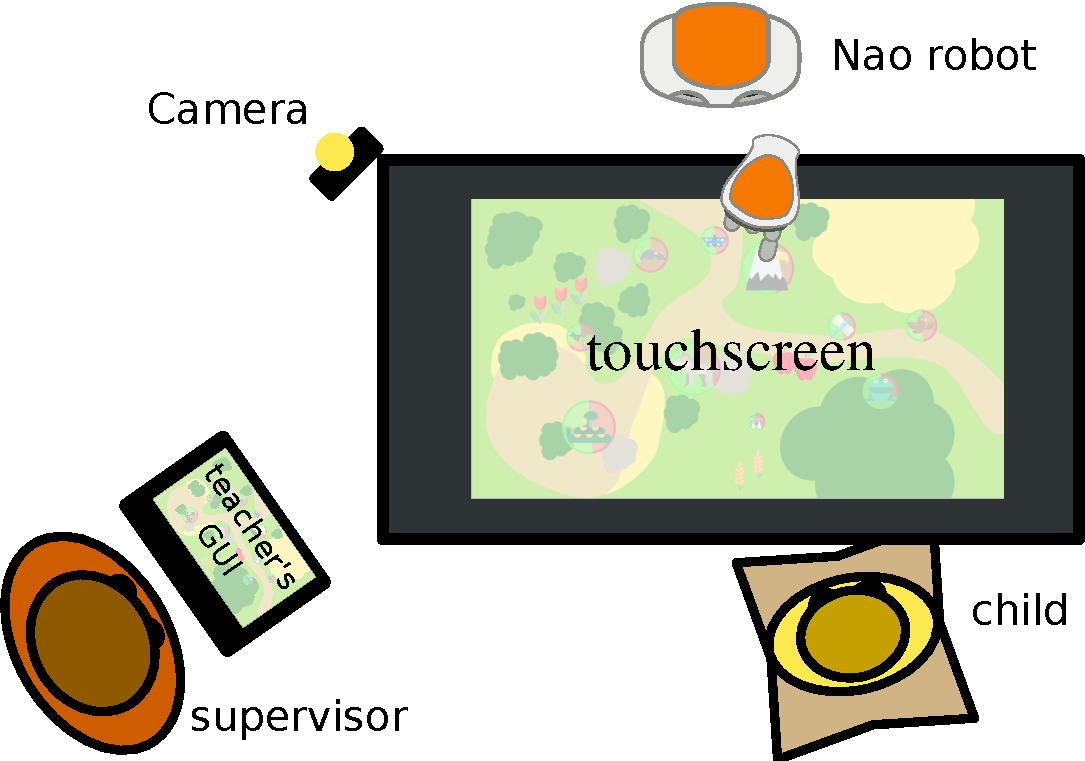
\includegraphics[width=.8\linewidth]{setup.pdf}
	\centering
	\caption{Frame of the interaction: a robot interacts with a target, suggests actions and receive commands and feedback from a teacher. The robot uses machine learning to improve its suggestions over time.}
	\label{fig:frame}
\end{figure}

\section{Principles} \label{sec:sparc_principles}

\gls{sparc} defines an interaction between a learner (virtual agent or robot) and a teacher following these principles:
\begin{itemize}
	\item The learner has access to a representation of the state of the world and a set of actions.
	\item The teacher can select actions for the robot to execute.
	\item The learner can propose actions to the teacher before executing them (informing them about its intentions) .
	\item The teacher can enforce or cancel actions proposed by the learner and actions non evaluated are implicitly validated and executed after a short delay.
	\item The learner uses \gls{ml} to improve its action policy using the teacher's commands and feedback on propositions.
\end{itemize} 

This interaction between the learner and the teacher is similar to the level 6 on the Sheridan scale of autonomy: "computer selects action, informs human in plenty of time to stop it" \citep{sheridan1978human} with the addition that the human has the opportunity to select actions for the agent to execute. In this thesis, we will refer to this interaction as `\gls{sa}': the robot interacts autonomously under the supervision of a human who can ensure that the behaviour is constantly appropriate.

This way of keeping a human in the learning loop and with the opportunity to override the agent actions and the robot learning from these demonstrations is similar to Dogged Learning \citep{grollman2007dogged}. However, with \gls{sparc}, this ability to provide demonstrations is combined with \gls{sa}. This results in a mixed control system where the teacher can select actions and have the robot perform them while the robot only proposes actions to the teacher. In response to this suggestion, the teacher has the choice between pre-empting the action or let it be executed. A learning algorithm on the robot side uses the feedback and commands from the teacher to improve the correctness of the suggested actions until reaching an efficient action policy. This learning mechanism coupled with auto-execution of actions aims to decrease over time the requirement of interventions from the teacher, thus reducing the workload on the teacher as the robot learns. The diagram presented in Figure \ref{fig:sparc_diagram} and the flowchart in Figure \ref{fig:sparc_flowchart} present in a graphical way this interaction between the learner and the teacher.

\begin{figure}[ht]
	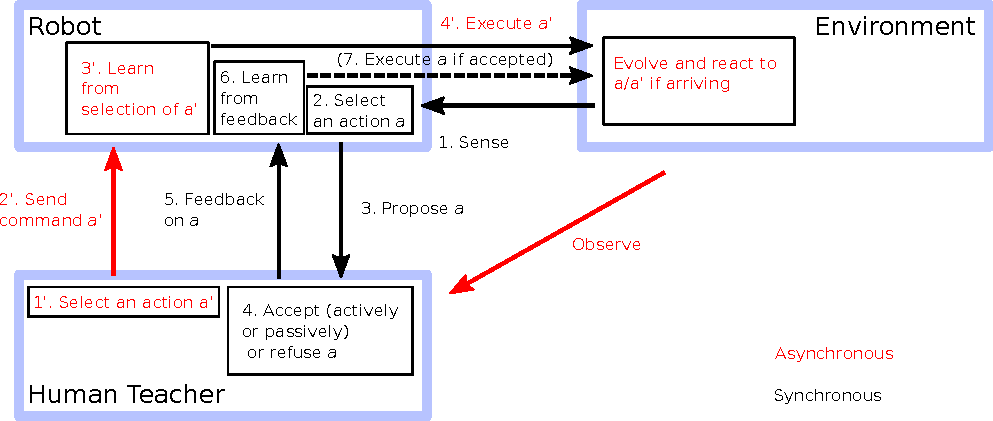
\includegraphics[width=1\linewidth]{diagram.pdf}
	\centering
	\caption{Diagram of interaction between the robot, the human teacher and the environment with \gls{sparc}: synchronously, the robot can propose actions to the teacher that evaluated (approved or cancelled) and the teacher can select actions to be executed in an asynchronous fashion.}
	\label{fig:sparc_diagram}
\end{figure}

Additionally, keeping the human in the loop also gives them the opportunity to provide additional information to the algorithm speeding up the learning. The main difference between \gls{sparc} and Dogged Learning or CBA \citep{chernova2009interactive} is the communication of intentions and full control of the teacher over the robot's action with \gls{sparc}. The teacher is informed beforehand of the robot future actions and can prevent them before the execution, which provides more control on the robot's action policy compared to other \gls{iml} methods. The teacher does not have to correct an action after it has impacted the world, but can pre-empt incorrect actions using the intention or suggestion transmitted by the robot. The agent learns to avoid actions with expected negative impact without having to face the results of the execution of these undesired actions. This implies that the behaviour executed by the robot can be assumed to be optimal, potentially simplifying the learning mechanism.

\begin{figure}[ht]
	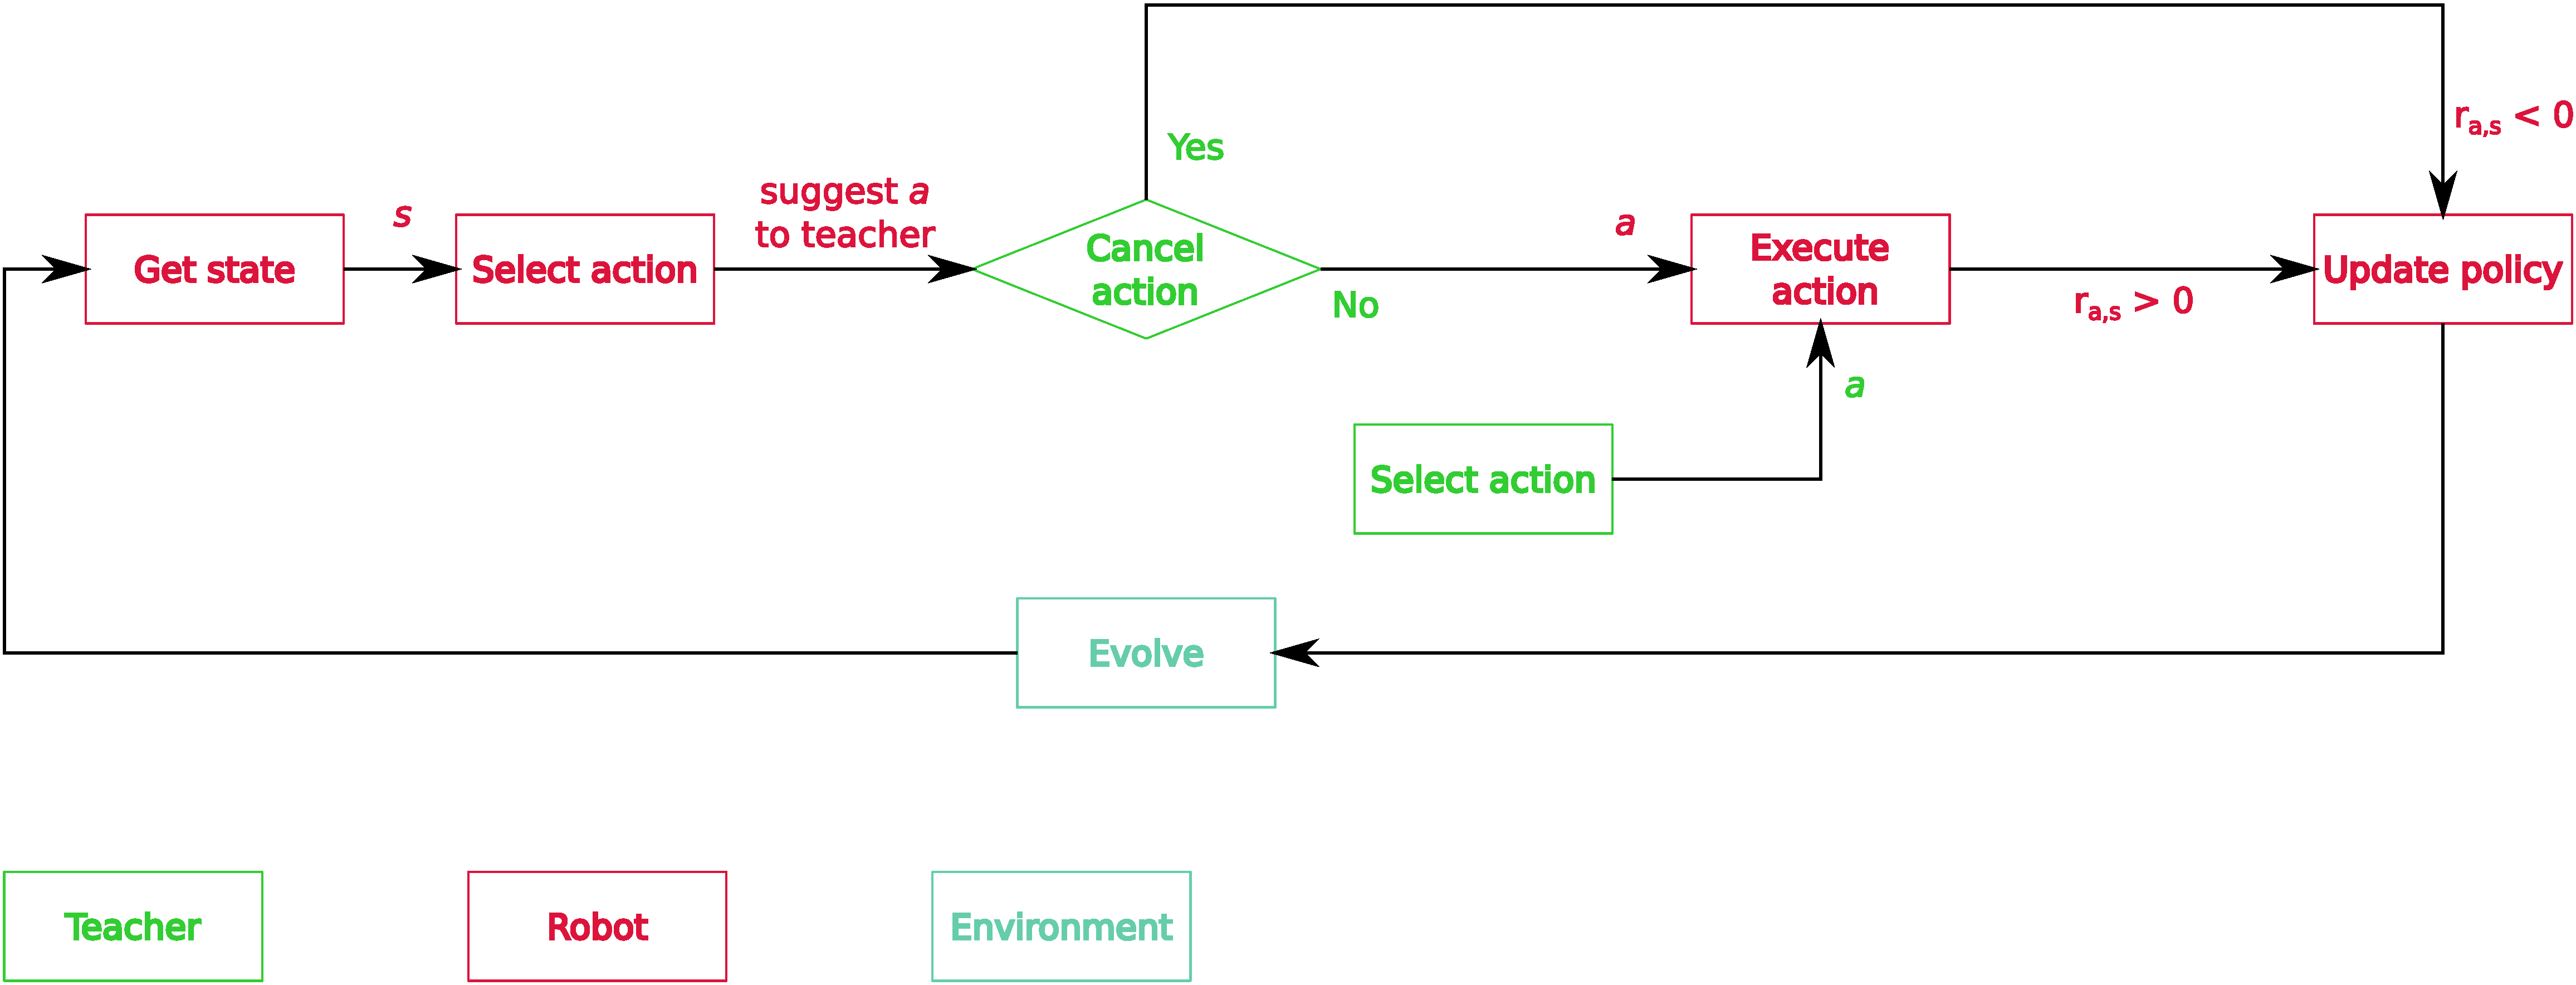
\includegraphics[width=1\linewidth]{flowchart.pdf}
	\centering
	\caption{Flowchart of the action selection loop between the robot and the teacher.}
	\label{fig:sparc_flowchart}
\end{figure}

This approach is comparable to predictive texting as seen on phone nowadays. The user can select the words proposed by the algorithms (or implicitly accept them by pressing space) or write their own. The algorithm learns the user's preferences and habits and aims to suggest words more and more appropriate to the user. However, predictive texting aims mostly to correct users' errors and interact in static environments. And \gls{sparc} aims to replicate a teacher's action policy in continuous time, in a dynamic interactive environment evolving both dependently and independently of the agent actions.

Alternatively, \gls{sparc} can be seen as a way to provide pro-activity to the robot. By observing interactions on a larger time scale, such as an assistant robot at home, \gls{sparc} allows the agent to propose help when the current state is similar to previous observation. This would be to compare to an operated robot where each action executed by the robot would have to be requested by the user. By proposing actions to the teacher, the robot takes the initiative to support humans, while not imposing its presence in the environment: executing actions without informing the surrounding humans could be perceived as rude or annoying.

\section{Goal}

\gls{sparc} aims to provide an interaction framework to teach robots an action policy possessing the following characteristics:
\begin{itemize}
	\item Usable by people without expertise in computer science.
	\item Fast policy learning from in-situ guidance.
	\item No constant requirement of human input to act in the world.
	\item Robot's behaviour constantly appropriate.
\end{itemize}

Figure \ref{fig:concept} presents an idealistic comparison of the expected workload, performance and autonomy of four methods: autonomous learning (e.g. \gls{rl} - \citealt{sutton1998reinforcement}), feedback based teaching (e.g. TAMER - \citealt{knox2009interactively}), \gls{woz} and \gls{sparc}. Unlike other methods, by following the principles presented in Section \ref{sec:sparc_principles}, \gls{sparc} is expected to maintain a constant high performance even during early stages of learning. In later stages of the learning, the workload on the human teacher should decrease as the agent improves its action policy, making its suggestions more accurate.

\begin{figure}[ht]
	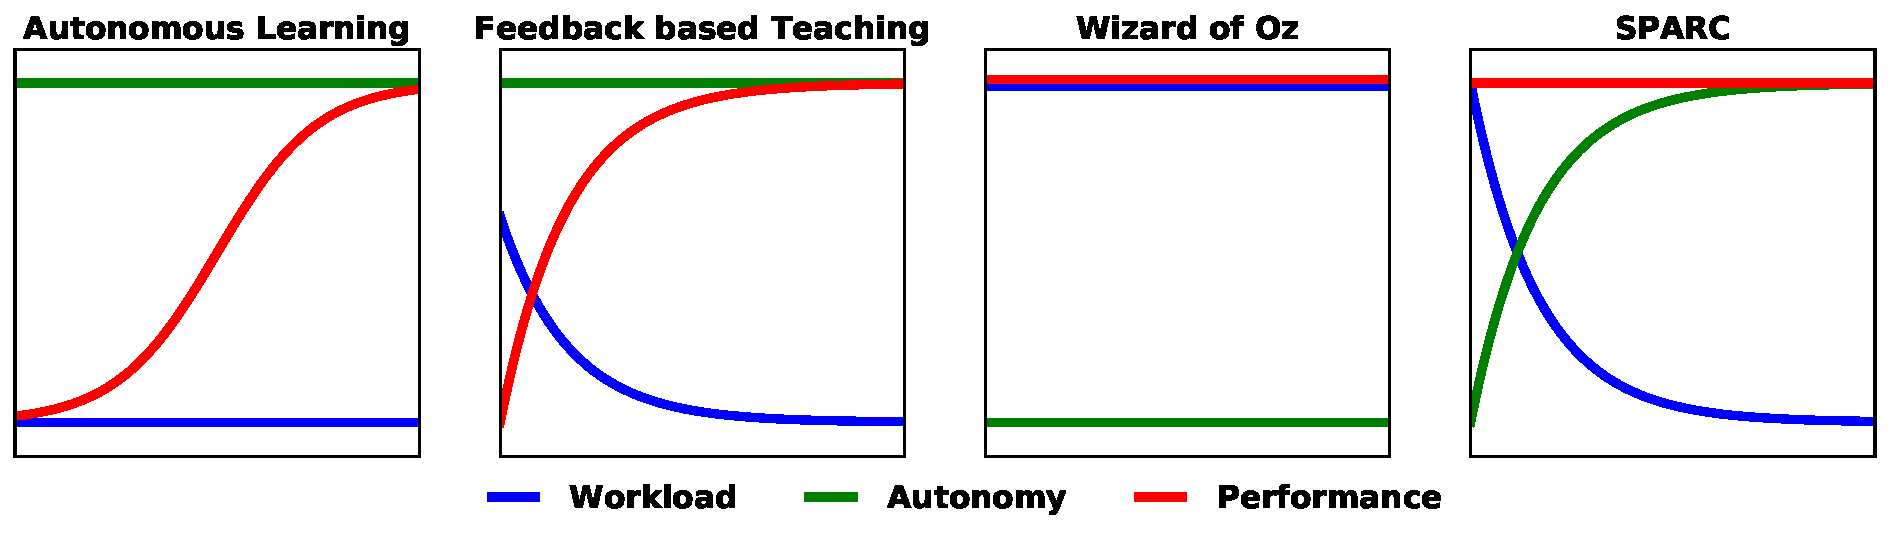
\includegraphics[width=1\linewidth]{concept.pdf}
	\centering
	\caption{Idealistic evolution of workload, performance, and autonomy over time for autonomous learning, feedback-based teaching, \gls{woz} and \gls{sparc}.}
	\label{fig:concept}
\end{figure}

Once the behaviour is deemed appropriate enough by the teacher, the agent is ready to be deployed to interact autonomously in the real world if this outcome is desired. Alternatively, in contexts where a human expert still cannot be removed from the control loop, such as \gls{rat}, a supervisor stays in control of the robot's actions in a \gls{sa} fashion. Similarly to the teaching phase, the robot informs the supervisor of its actions and the human only has to intervene in case of incorrect propositions. While still requiring attention from the supervisor, this reduction of human actions to control the robots aims at reducing the workload on the supervisor. As the supervisor has a better knowledge of the agent's behaviour, they can be especially careful in cases when they know the agent is prone to making errors. And as the control of the agent requires less effort from the supervisor, they can focus more closely on the application interaction than the teaching one in the other cases. 
%This approach is similar to safety drivers behind autonomous vehicles but with information about the car's intentions rather than solely observing the car's actions. 
%MAybe something on knowing critical parts of the interaction policy (Example DREAM only evaluation of performance)

\section{Implications}

Similarly to other \gls{iml} approaches, the requirement of a human in the action selection loop limits the time scale of interaction and this effect is an important consideration when applying \gls{sparc} to an interaction. With this type of \gls{iml}, three time scales are coexisting: the robot's, the teacher's and the interaction's. The robot has an internal clock running probably multiple times per second, sensing the world and deciding if an action should be provided. The human teacher has to be able to cancel actions before their executions, so they needs to be provided with few seconds to react to propositions, which reduces the rate of actions selection to 0.5 Hz or below. Depending of the application, actions might have to be executed in a time critical environment (such as driving) or less critical ones (such as an assistant robot at home supporting a person). This means that the width of actions' acceptance window impacts the usability of \gls{sparc}. To be applicable, an acceptance window needs to span few seconds to have the actions being valid both when proposed by the robot and when accepted by the teacher. The difference of time scales and the requirement of time allocated for the teacher to react reduce the application of \gls{sparc} compared to other \gls{iml} methods. However, this limitation of application is the price to pay to ensure the appropriateness of actions, and this effect can be mitigated by using higher level actions or applications less critical in term of time.  % and this has the advantage to ensure that only correct actions will be executed without requiring the human to select them all.

\gls{sparc} is an \gls{ilfd} method (cf Section \ref{ssec:back_ilfd}) and as such presents many similarities with other non-interactive \gls{lfd} (cf. Section \ref{ssec:back_lfd}) as it uses human demonstrations of policies to learn. However, most of the applications of \gls{lfd} \citep{argall2009survey,billard2008robot} are focused on learning a manipulation skill in a mostly deterministic environment. \gls{lfd} has seldom been used to teach an action policy to interact with humans \citep{liu2014train,sequeira2016discovering,munzer2017efficient} and never in an online fashion. Munzer et al. proposed an interactive planner that would learn offline the current user's preferences and desires, but two key differences exist between this approach and \gls{sparc}. The learning planner is well suited to clearly defined environments (e.g. \gls{hrc}) where a similar task with clear steps has to be done multiple times. As such the learning can happen offline between the repetitions. \gls{sparc} is defined to be applicable to non-linear environments where learning should happen online in tasks without clear start and ending states. Secondly, using a threshold, Munzer et al. define actions with low risk which are executed (and can be cancelled during the execution) and actions with higher risk which have to be validated first by the human. \gls{sparc} does not make this distinction, but proposes both types of actions to the teacher and will start executing them if no feedback is received. This removes the  need for the human to explicitly approve a correct action if proposed while ensuring that the human can cancel incorrect action before their execution. This principle aims to reduce the number of required interventions from the human to teach the robot compared to methods as the one presented by Munzer et al. 

Additionally, \gls{sparc} differs from Active Leaning (cf. Section \ref{ssec:back_active}) by the fact that the agent cannot decide which sample will be evaluated by the teacher. As the robot interacts with humans, the datapoints provided to the teacher for \textit{labelling} emerge from the interaction, and cannot be selected at will. 
    
%\section{Implications}

%The principles described in section \ref{sec:sparc_principles} have also implications on the interactions between the teacher and the agent and between the agent and the environment. As the teacher has the power evaluate the actions proposed by the agent before their execution, it actually evaluates the intentions of the agent rather than its behaviour. This difference is key as traditional \gls{iml} approaches only evaluate the actions a posteriori by their effects. This implication is fundamental in \gls{hri} as a robot executing non appropriate actions when interacting with humans should not be deployed (cf. first principle in Section \ref{ssec:back_constraints}) and asing the evaluation of the teacher on the intention rather than waiting for the action's outcome gives the opportunity to the teacher to pre-empt incorrect actions preventing the execution of undesired behaviours. The agent learns to avoid actions with expected negative impact without having to face the results of the execution of these undesired actions.

%Most importantly, the control given to the teacher on the agent's actions ensures that every action executed by the learner in the world has been either actively or passively validated by the teacher. This implies that each action executed can be assumed to be appropriate to the current state, potentially simplifying the learning algorithm.

\section{Interaction with Machine Learning Algorithms}

The principles of \gls{sparc} define it at the crossroads between \gls{sl} and \gls{rl}. \gls{sparc} can be used in two ways: either to reproduce a teacher's policy in a supervised fashion or to discover a useful action policy using the teacher to bias the exploration, limiting errors and only interacting in desired parts of the environment.

As such, \gls{sparc} only defines an interaction framework between a teacher and a learner, and is agnostic to the learning mechanism: it can be combined with any algorithms used in \gls{sl} or \gls{rl}. This research explored combinations with three types of algorithms: supervised learning using a feed-forward neural network (Chapter \ref{chap:woz}), reinforcement learning (Chapter \ref{chap:control}), and supervised learning using an instance based algorithm (Chapter \ref{chap:tutoring}). However \gls{sparc} could be combined with a wide range of other algorithms.


Similarly to Inverse Reinforcement Learning \citep{abbeel2004apprenticeship} or other techniques combining \gls{rl} and \gls{lfd} \citep{billard2008robot}, if used with a reward function \gls{sparc} could go beyond the demonstrated action policy and achieve a performance higher than the demonstration. However this aspect has not been evaluated in this work.

\section{Summary}
    
This chapter introduced \acrfull{sparc}, a novel interaction framework to teach agents an action policy. This approach is suited to teach a robot to interact with humans as it validates the principles defined in Section \ref{ssec:back_constraints}. \gls{sparc} starts in a similar fashion to \gls{woz}: the teacher selects actions at any time to be executed by the robot. Then, using a learning algorithm, the agent starts to propose actions to the teacher who can let them be executed after a short time or cancel them if not appropriate. This mechanism combining selections, suggestions, and evaluations ensures the appropriateness of actions as a human could have pre-empted any inappropriate action before their execution. This additionally provides the adaptivity as the teacher can extend the behaviour beyond the current action policy. The learning algorithm associated with the auto-executions ensures that once the robot starts to learn, the human workload decreases. When an acceptable action policy is reached, the robot is ready to be deployed to interact autonomously if this outcome is desired.

\cleartooddpage

\chapter[Study 1: Comparison Between SPARC and WoZ]{Study 1: \\ Comparison Between SPARC and WoZ}\label{chap:woz}
\glsresetall
\graphicspath{{images/woz/}}

\begin{framed}
	\textbf{Key points:}
	
	\begin{itemize}
		\item Design of an experiment to explore the influence of \acrshort{sparc} on the teacher's workload and task performance compared to an approach based on \acrshort{woz}.
		\item Application target replaced by a robot to ensure repeatability of the target behaviour.
		\item Design of a robot model exhibiting probabilistic behaviour (simulating a child) with a non-trivial optimal interaction policy.
		\item Results from a within subject study involving 10 participants show that \acrshort{sparc} achieves a similar performance than \acrshort{woz} while requiring a lower workload from the teacher.
	\end{itemize}
\end{framed}

Parts of the work presented in this chapter have been published in \cite{senft2015sparc}. The final publication is available from Springer:
\begin{itemize}
	\item SPARC: Supervised	Progressively Autonomous Robot Competencies. In International Conference on	Social Robotics\footnote{\url{http://dx.doi.org/10.1007/978-3-319-25554-5_60}}.
\end{itemize} 

Technical contribution in this chapter: the author used software from the \acrshort{dream} project for the touchscreen and the robot functionalities. The author contributed to the material used within the robot control and the Graphical User Interface. Algorithm used from the OPENCV neural network library.

\newpage

\section{Motivation}

The \gls{sparc} has been designed to enable end-users without expertise in computer science to teach a robot an action policy while interacting in a sensitive environment, such as \gls{hri}. By using machine learning and \gls{sa}, \gls{sparc} intends to allow a field expert to progressively transfer their knowledge to an autonomous agent without having to enforce each action manually. Additionally, as the agent is interacting in the target environment, displaying an appropriate action policy, the time spent to teach it is not lost but used to deliver the desired interaction even during the learning phase. For example, in the context of \gls{rat}, a therapist would teach the robot during therapy sessions. And, as the therapist is in total control of the robot's action, the behaviour expressed by the robot always fits the  desired goals for the therapy. This ensures that even the sessions used to teach the robot have a therapeutic value for the patient involved in the therapy.

\gls{sparc}, as a principle, allows to start a robotic application in a \gls{woz} fashion and then move away from it as the robot gains autonomy. The aim of \gls{sparc} is twofold: maintaining a high level of performance in the target application while reducing the workload of the teacher over time. As the robot learns, the action policy is refined until reaching a point where the robot is autonomous or only necessitates minimal supervision to interact successfully. 

As explained in Chapter~\ref{chap:sparc}, \gls{sparc} involves two interactions: the teaching interaction and the application one (see Figure~\ref{fig:woz_setup_diag}). As such, when the goal of the teaching is interacting with humans, the robot interacts simultaneously with at least two humans (the target(s) and the teacher). These two dependent interactions add complexity to the evaluation of the approach, especially as both humans are impacting each other. 

The first step to evaluate \gls{sparc} was to focus on the teaching interaction, the relation between the robot and its teacher. To evaluate this aspect of the interaction, we decided use the context of \gls{rat} for children with \gls{asd}. However, as the presence of two humans decrease the repeatability of the test benchmark, we replaced the child involved in the therapy by a robot running a model of a child. The setup ends up with two robots interacting together: the \emph{child-robot} completing a therapeutic task and the \emph{wizarded-robot}, controlled by a participant (taking the role of the teacher), supporting the child-robot in its task completion (cf. Figure~\ref{fig:woz_setup_diag}). Actions from the wizarded-robot impact the child-robot's behaviour and to achieve a high performance in the task, the child-robot needs to receive an efficient supporting policy from the wizarded-robot. As such, the child-robot's performance is used as a proxy to evaluate the performance of the participant in the supervision. This environment with a single human-robot interaction allows us to observe and evaluate the impact of \gls{sparc} on the teaching interaction, while controlling for variable interactions with the target.

\begin{figure}[ht]
	\centering
	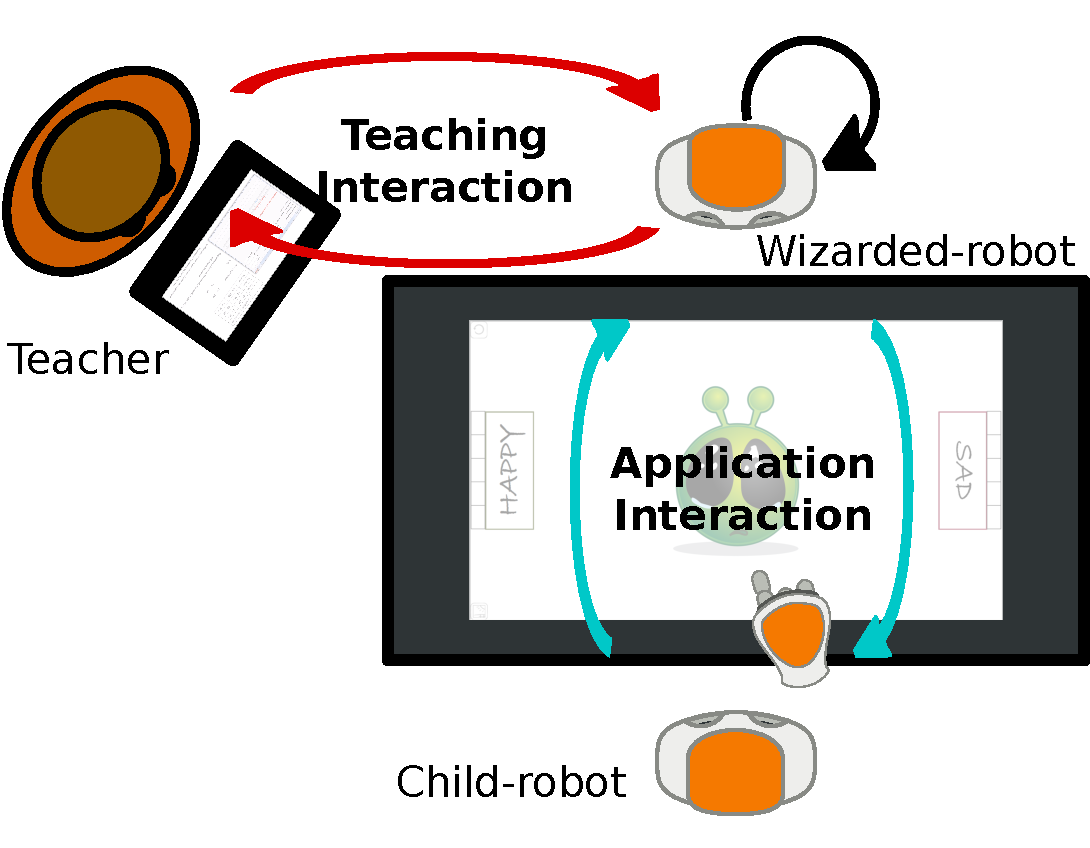
\includegraphics[width=.8\textwidth]{setup_diag.pdf}
	\caption{Setup of the interaction. The application target, a child has been replaced by a robot for repeatability.}
	\label{fig:woz_setup_diag}
\end{figure}

\section{Scope of the Study}
%\ES{mention the RQ?}
The study presented in this chapter intends to evaluate if the learning component of \gls{sparc} could allow participants to teach an efficient action policy for a robot interacting with humans. For repeatability concerns, the human-robot interaction target of the learning has been modelled by another robot with a complex but repeatable behaviour. The control condition is a variation of \gls{woz}, where participant still control a robot but without the learning component. By combining learning and \gls{sa}, \gls{sparc} aims to allow the teacher to maintain a high performance during the interaction while reducing the workload on the teacher over time.

To evaluate the validity of \gls{sparc} and the influence of such an approach, four hypotheses were devised:
\begin{enumerate}
	\item [H1] The child-robot's performance is a good proxy for the teacher's performance (there is high correlation between the child-robot performance and the teacher performance - maintaining the child-robot internal states high).
	\item [H2] When interacting with a new system, humans progressively build a personal strategy that they will use in subsequent interactions (resulting in variable teacher's outputs and improving their performance in successive interactions).
	\item [H3] Reducing the number of interventions required from a teacher reduces their perceived workload.
	\item [H4] Using \gls{sparc} allows the teacher to achieve similar performance than \gls{woz} but with a lower workload.
\end{enumerate}

H1 represents a validation of the model, ensuring that the child-robot performance represents the efficiency of the action policy applied by the teacher. H2 tests that human teachers are not static entities, they adapt their teaching target and their interaction strategy based on their knowledge and understanding of the task. H3 tests one of the motivations behind \gls{sparc}: does reducing the number of physical actions from a human to control a robot while requiring the teacher to monitor the robot suggestions lead to a lower perceived workload. Finally, H4 is the main hypothesis, does \gls{sparc} enables a robot to learn a useful action policy: reducing the teacher's workload while maintaining a high performance.

\section{Methodology}

\subsection{Participants}

The study involved 10 participants (7M/3F, age \textit{M}=29.3, 21 to 44, \textit{SD}=4.8 years). While \gls{sparc} is expected to be usable by anyone, regardless of their knowledge of computer sciences, this first study involved members of a robotic research group assuming the role of the robot supervisor. This decision is supported by the fact that in \gls{rat} scenarios, the wizard is typically a technically competent person with significant training controlling this robot for this therapy. As such, as the participants come from a population expected to assume this type role, the results of the study maintain their applicability to \gls{hri}.

\subsection{Task}

This study is based on a real scenario for \gls{rat} for children with \gls{asd} based on the Applied Behaviour Analysis therapy framework~\citep{cooper2007applied}. The aim of the therapy is to help a child to develop/practice their social skills by completing tasks with a human or robotic partner. The child has to complete an emotion recognition task by playing a categorisation game with a robot on a mediating touchscreen device~\citep{baxter2012touchscreen}. The robot can provide feedback and prompts to encourage the child and help them to classify emotions. In the task, images of faces or drawings are shown to the child on the touchscreen, and the child has to categorise them by moving them to one side of the screen or the other depending on whether the picture shown denotes happiness or sadness. In real therapies, the robot would be generally remote-controlled by an operator using \gls{woz}~\citep{riek2012wizard}.%, and does not interact with the child directly. 

This study explores if \gls{sparc} can be used to teach the robot a correct action policy to support the child in this therapy scenario. As timing in human-robot interactions is complex, for simplification reasons, the interaction has been made discrete to have clear steps when the robot has to execute an action. During these action steps, the selection of an action is decided by following the principles defining the \gls{sa}:
\begin{enumerate}
	\item The robot suggests an action to the teacher.
	\item The teacher can select an action for the robot to execute or let the proposed action be executed after a short delay.
	\item The robot executes the selected action.
	\item Both the robot and the teacher observe the outcome of the action until the next action selection step.
\end{enumerate}

%Using \gls{sparc}, the robot learns over time to replicate the teacher's policy by matching the inputs (child's state) to the outputs (action selected by the teacher). 

%the policy used by the teacher based on observations of the child and the oversight from the teacher, with the teacher still maintaining overall control if necessary.

This study compares two conditions: \gls{sparc}, where the robot learns from the human selections and the \gls{woz} condition where the robot is simply controlled by the participant. As mentioned before, in both conditions, actions can only be executed in predefined time windows dictated by the dynamics of the interaction. Additionally, a `wait' action is present in the \gls{sparc} condition and presents an active choice for the participants. 
In a real \gls{woz} scenario, participants would have to enforce every single action made by the robot, however, a `wait' action in that context does not make sense. As such, in the \gls{woz} condition, the robot proposes random actions, thus increasing the probability of having the teacher correcting the suggestion leading up to a setup similar to a real \gls{woz}. This random behaviour is also the starting point of the \gls{sparc} condition.

As mentioned earlier, the focus of the study being on the teaching interaction (the relation between the teacher and the robot), the second interaction (the application) has been kept constant by replacing the child by a robot. A minimal model of child behaviour is therefore used to stand in for a real child. A second robot is employed in the interaction to embody this child model: we term this robot the \textit{child-robot} while the robot being directly supervised by the human teacher is the \textit{wizarded-robot} (cf. Figure~\ref{fig:woz_setup}).

\begin{figure}[ht]
	\centering
	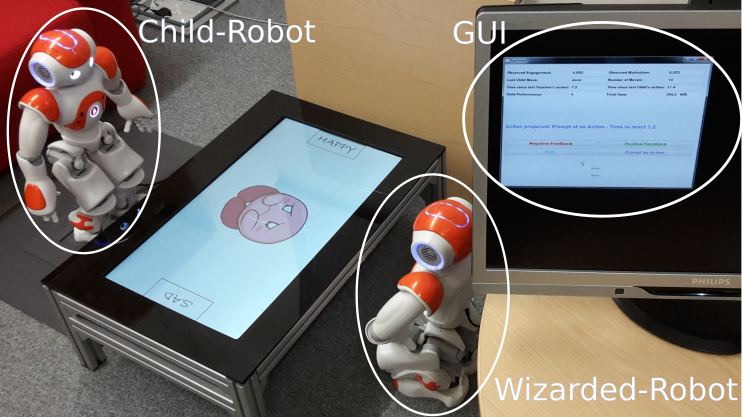
\includegraphics[width=.9\textwidth]{setup_annotated.png}
	\caption{Setup used for the user study from the perspective of the human teacher. The child-robot (left) stands across the touchscreen (centre-left) from the wizarded-robot (centre-right). The teacher can oversee the actions of the wizarded-robot through the \gls{gui} and intervene if necessary (right).}
	\label{fig:woz_setup}
\end{figure}
		
\subsection{Child Model} \label{ssec:woz_child}

The purpose of the child model is not to realistically model a child (with or without autism), but to provide a means of expressing some characteristics of the behaviours we observed in interactions with children in a repeatable manner. The child-robot possesses an internal model encompassing an engagement level and a motivation level. Together these form the state of the child. The engagement represents the involvement of the child in the task, i.e. how often the child-robot will make categorisation moves. And the motivation relates to the seriousness of the child in solving task; in the model, the motivation gives the probability of success of each categorisation move. 

These states are bound to the range [-1, 1] and influenced by the behaviour of the wizarded-robot. Values of 1 indicate that the child-robot's behaviour is positive, it is involved in the task. Values of -1 show that the child-robot is actively refusing to participate. And a 0 represents a neutral state where the child-robot is neither especially involved nor actively disengaged. To represent a tendency to return to a neutral state of mild engagement, both states asymptotically decay to zero with no actions from the wizarded-robot. These two states are not directly accessed by either the teacher or the wizarded-robot, but can be observed through behaviour expressed by the child-robot: low engagement will make the robot look away from the touchscreen, and the speed of the categorisation moves is related to the motivation (to which gaussian noise was added). There is thus incomplete/unreliable information available to both the wizarded-robot and the teacher.

As explained in Section~\ref{ssec:woz_wizarded_robot}, the wizarded-robot's action impact the child-robot state: congruent action will tend to increase engagement and motivation. However, if repeated, actions can lead to frustration for the child-robot. If a state is already high and an action from the wizarded-robot should increase it further, there is a chance that this level will sharply decrease. When this happens, the child-robot will indicate this frustration verbally by uttering one of eight predefined strings. This mechanism prevent the optimal strategy to be straightforward: always making actions aiming to increase motivation or engagement. The optimal strategy combines feedback actions and waiting ones to maintain the state values high but prevent them from overshooting. This non-trivial optimal action policy approximates better a real human-robot interaction scenario requiring a more complex strategy to be expressed by the robot.

\subsection{Wizarded-Robot Control}
\label{ssec:woz_wizarded_robot}
The wizarded-robot is controlled through a \gls{gui} (shown in Figure~\ref{fig:woz_gui}) and has access to the variables defining the state of the interaction used by the learning algorithm:
\begin{itemize}
	\item Observed engagement.
	\item Observed motivation.
	\item Type of last categorisation made by the child-robot (good/bad/done).
\end{itemize}

\begin{figure}[ht]
	\centering
	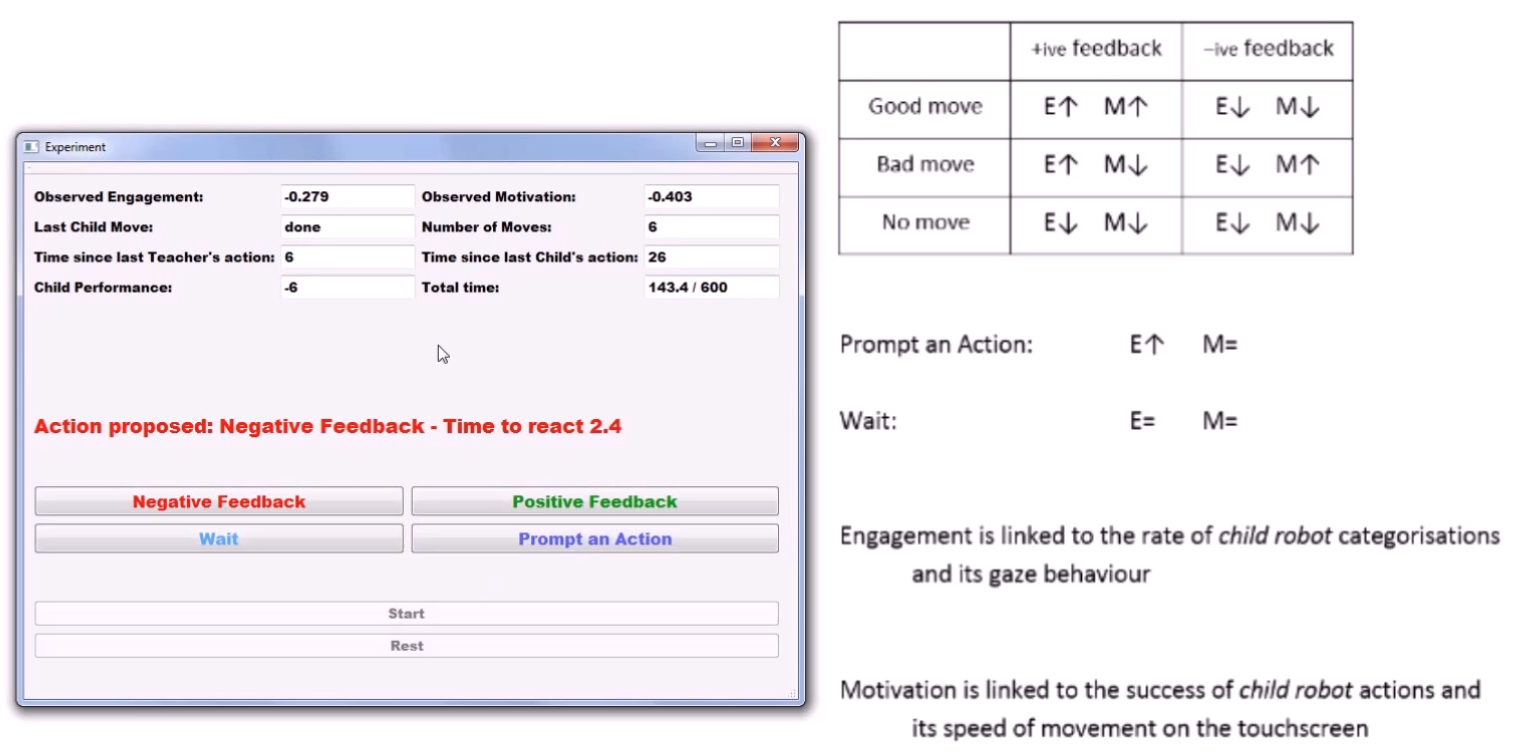
\includegraphics[width=1\textwidth]{GUI-woz.png}
	\caption{Screenshot of the interface used by the participants, the \gls{gui} on the left allows to control the robot and a summary of the actions' impact is displayed on the right.}
	\label{fig:woz_gui}
\end{figure}

Additionally, other metrics are displayed to the teacher but not used by the algorithm:
\begin{itemize}
	\item Number of categorisations made by the child-robot.
	\item Time since teacher's last action.
	\item Time since child-robot's last action.
	\item Child-robot's performance.
	\item Total time elapsed.
\end{itemize}


The wizarded-robot has a set of four actions it can execute, each represented by a button on the \gls{gui}: 
\begin{itemize}
	\item \textbf{Prompt an Action}: Encourage the child-robot to do an action.
	\item \textbf{Positive Feedback}: Congratulate the child-robot on making a good classification.
	\item \textbf{Negative Feedback}: Supportive feedback for an incorrect classification.
	\item \textbf{Wait}: Do nothing for this action opportunity, wait for the next one.
\end{itemize}


The impact of actions on the child-robot depends on the internal state and the type of the last child-robot move: good, bad, or done (meaning that feedback has already been given for the last move and supplementary feedback is not necessary). A \textit{prompt} increases the engagement, a \textit{wait} has no effect on the child-robot's state, and the impact of positive and negative feedback depends on the previous child-robot move. Congruous feedback (positive feedback for correct moves; negative feedback for incorrect moves) results in an increase in motivation, but incongruous feedback can decrease both the motivation and the engagement of the child-robot. The teacher therefore has to use congruous feedback and prompts.

However, as mentioned in Section~\ref{ssec:woz_child}, if the engagement or the motivation exceeds a threshold, their value can decrease abruptly to simulate the child-robot being frustrated. This implies that the optimal action policy consist on providing congruous feedback and prompts, but also requires wait actions to prevent the child-robot from becoming frustrated and maintain its state-values close to the threshold without exceeding it. However, as the participants do not know the parameters of the models running on the child-robot and do not have access to the exact state values, this optimal policy is not available to participants. A `good' strategy keeping the engagement and motivation high leads to an increase in performance of the child-robot in the categorisation task.

As introduced previously, to simplify the algorithm part, the interaction has been discretised, the teacher cannot select actions for the wizarded-robot at any time. Actions can only be executed at specific times triggered by the wizarded-robot: two seconds after each child-robot categorisation or if nothing happened for five seconds since the last wizarded-robot's action. When these selection windows are hit, the wizarded-robot proposes an action to the teacher by displaying the action's name and a countdown before execution. The teacher can only select an action in reaction to a proposition from the wizarded-robot; alternatively, if the teacher does nothing in the three seconds following the suggestion, the action proposed by the wizarded-robot is executed. This mechanism allows the teacher to passively accept a suggestion or actively intervene by selecting a different action and forcing the wizarded-robot to execute it.

\subsection{Learning Algorithm}

In the \gls{sparc} condition, the robot learns to reproduce the action policy displayed by the teacher. For this study, the algorithm is of incidental importance, any algorithm could have been used, but as only supervised learning is required, we used a Multi-Layer Perceptron (MLP) with five input nodes: one for the observed motivation, one for the observed engagement and three binary (+1/-1) inputs for the type of the previous move: good, bad, or done. The hidden layer had six nodes and the output layer four: one for each action. The suggested action is selected applying a Winner-Take-All strategy on the value of the output node and then displayed on the \gls{gui} before execution. The network is trained with back propagation: after each new decision from the teacher a new training point is added with the selected action node having +1 while the others are set to -1. The network is fully retrained with all the previous state-action pairs and the new one between each selection step. 
%The network was using sigmoid activation function and a learning rate of 0.6 (probably).

This learning algorithm, MLP, is not optimal for online learning for real time interactions as the learning should happen quickly between learning iterations. However, as the length of interaction (and so the number of datapoints) is limited, the network can be retrained between consecutive uses. Finally, the desired learning behaviour being purely supervised learning, this type of algorithm has been deemed suitable for this study.
%On the other side, the random controller proposed random actions to the teacher.

\subsection{Interaction Protocol}

The study compared two conditions: a learning robot adapting its propositions to its user (the \gls{sparc} condition) and a non-learning robot constantly proposing random actions (the \gls{woz} condition). The child-robot controller was kept constant in both conditions, while the state was reset between interactions. The study used a within subject design with balancing of order: each participant interacted with both conditions, and the order of interaction has been balanced between participants to control for any ordering effects. In the order S-W the participants first interact with the learning wizarded-robot in the \gls{sparc} condition, and then with the non-learning one in the \gls{woz} condition; and in the order W-S, this interaction order is inverted (starting with \gls{woz} then \gls{sparc}). Participants were randomly assigned to one of the two orders.

The interactions took place on a university campus in a dedicated experiment room. Both robots were Aldebaran Nao, one of which had a label indicating that it was the child-robot. The robots faced each other with a touchscreen between them. The participant, assuming the role of the teacher, sat at a desk to the side of the wizarded-robot, with a screen and a mouse to interact with the wizarded-robot (fig.~\ref{fig:woz_setup}). Participants were able to see the screen and the child-robot.

A document explaining the interaction scenario was provided to participants with a demographic questionnaire. After the information was read, a 30s video presenting the \gls{gui} in use was shown to participants to familiarise them with the interface, without biasing them towards any particular control strategy. Then participants clicked a button to start the first interaction which lasted for 10 minutes. The experimenter was sat in the room outside of the participants' field of view. After the end of the first interaction, a post-interaction questionnaire was administered. Similarly, in the second part of the experiment, the participants interacted with the other condition and completed a second post-interaction questionnaire. Finally, a post-experiment questionnaire asked participants to explicitly compare the two conditions. All questionnaires and information sheet are available online\footnote{ \url{https://emmanuel-senft.github.io/experiment-woz.html}}.

\subsection{Metrics}

Two types of metrics have been recorded for this study: interaction data representing objective behaviours and performance of the participants and subjective data through questionnaires.

\subsubsection{Interaction Data}

The state of the child-robot and the interaction values were logged at each step of the interaction (at 5Hz). At each selection step, all of the human actions were recorded: acceptance of the wizarded-robot's suggestion, auto-execution and selection of another action (intervention) as well as the current state of the child-robot (motivation, engagement and performance). 

The first metric is the performance achieved by participants in each interaction. As the policy applied by the participants cannot be evaluated directly, the performance of the child-robot in the task (number of correct categorisations minus number of incorrect categorisations) is used as a proxy for the participant performance. H1 evaluates if this approximation is valid by analysing the relation between the performance of the child-robot and the value of its inner states. If a strong correlation is found, it would demonstrate that a good supervision policy (managing to keep the engagement and the motivation of the child-robot high) leads to a high performance. As such, this child-robot performance represents how efficient the action policy executed by the wizarded-robot was when controlled by a participant.

The second important metric is the intervention ratio: the number of times a user chooses a different action than the one proposed by the wizarded-robot, divided by the total number of executed actions. This metric represents how often on average a user had to correct the robot and could be related to the workload the user had to face to control the robot.

\subsubsection{Questionnaire Data}
 
Participants answered four questionnaires: a demographic one before the interaction, two post-interaction ones where they were asked to evaluate the last interaction with the robots and a post-experiment questionnaire where they had to compare the two conditions. All the rating questionnaires used seven item Likert scale. For clarity for participants, in the questionnaires the wizarded-robot is named `teacher-robot' (as it was `teaching' the child-robot).

Post-Interaction questions:
\begin{itemize}
	\item The child-robot learned during the interaction (Likert scale 1 to 7).
	\item The performance of the child-robot improved in response to the teacher-robot's actions (Likert scale 1 to 7).
	\item The teacher-robot is capable of making appropriate action decisions in future interactions without supervision (Likert scale 1 to 7).
	\item The teacher-robot always suggested an incorrect or inappropriate actions (Likert scale 1 to 7).
	\item By the end of the interaction, my workload was very light (Likert scale 1 to 7).
	\item What did you pay most attention during the interaction? (child-robot, touchscreen, \gls{gui}, other).
\end{itemize}

Post-experiment questions:
\begin{itemize}
	\item There was a clear difference in behaviour between the two teacher-robots (Likert scale 1 to 7).
	\item There was a clear difference in behaviour between the two child-robots (Likert scale 1 to 7).
	\item Which teacher-robot was better able to perform the task? (first, second).
	\item Which teacher-robot did you prefer supervising? (first, second).
\end{itemize}

\section{Results}

\subsection{Interaction Data}

Figure~\ref{fig:woz_comp} presents the aggregated results (collapsed between orders) for the performance and the final intervention ratio for both conditions. While the number of participants is not sufficient to compute descriptive statistics, overall interaction results seemed to show that both conditions lead to similar performance (\gls{sparc}: 32.6 (95\% CI [27.89,37.31]) - \gls{woz}: 31.4 (95\% CI [25.9,36.9])). As supported by the absence of overlap between the 95\% CI, the \gls{sparc} condition tended to require less interventions (intervention ratio: \gls{sparc}: 0.38 (95\% CI [0.29,0.47]) - \gls{woz}: 0.59 (95\% CI [0.52,0.67])). 

\begin{figure*}[ht]
	\centering
	\begin{subfigure}[ht]{0.5\textwidth}
		\centering
		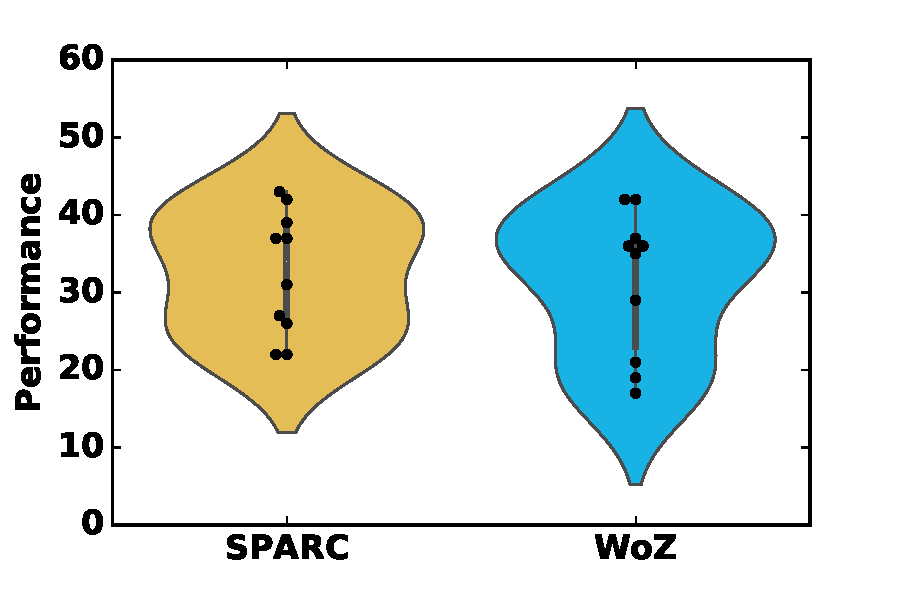
\includegraphics[width=1.0\textwidth]{perf.pdf}
%		\caption{Comparison of end performance for both conditions.}
	\end{subfigure}%
	~ 
	\begin{subfigure}[ht]{0.5\textwidth}
		\centering
		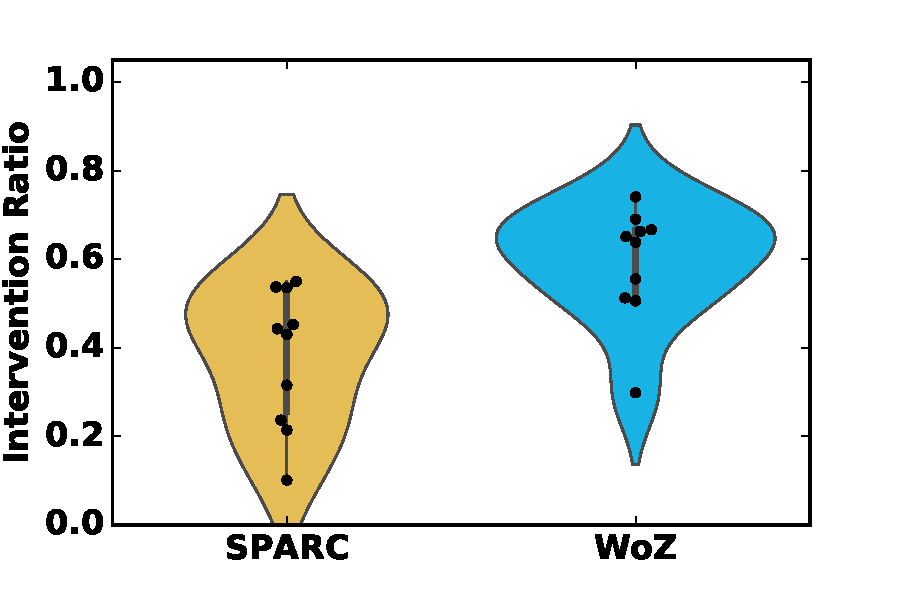
\includegraphics[width=1.0\textwidth]{ratio.pdf}
%		\caption{Comparison of intervention ratio for both conditions.}
	\end{subfigure}
	\caption{Aggregated comparison of performance and final intervention ratio for both conditions. Dots represent individual datapoint (N=10 per condition) and shaded area the probability distribution most likely to lead to these points.}
	\label{fig:woz_comp}
\end{figure*}

Figure~\ref{fig:woz_ratio_time} presents the evolution of intervention ratio for each condition, and their order. During the first interaction, participants discovered the interface and how to interact with it, which resulted in a high variation of the intervention ratio in the first 20 steps (with one step corresponding to one proposition of action from the wizarded-robot). However in the second phase of the interaction, when participants had developed their teaching policy, there was a tendency for \gls{sparc} to require a lower number of intervention than \gls{woz}. This effect was higher in the second interaction, where as soon as 5 steps, the two conditions differentiated without overlap of the 95\% CI of the mean. This would indicate that the two conditions differ in term of required interventions.

\begin{figure}[ht]
	\centering
	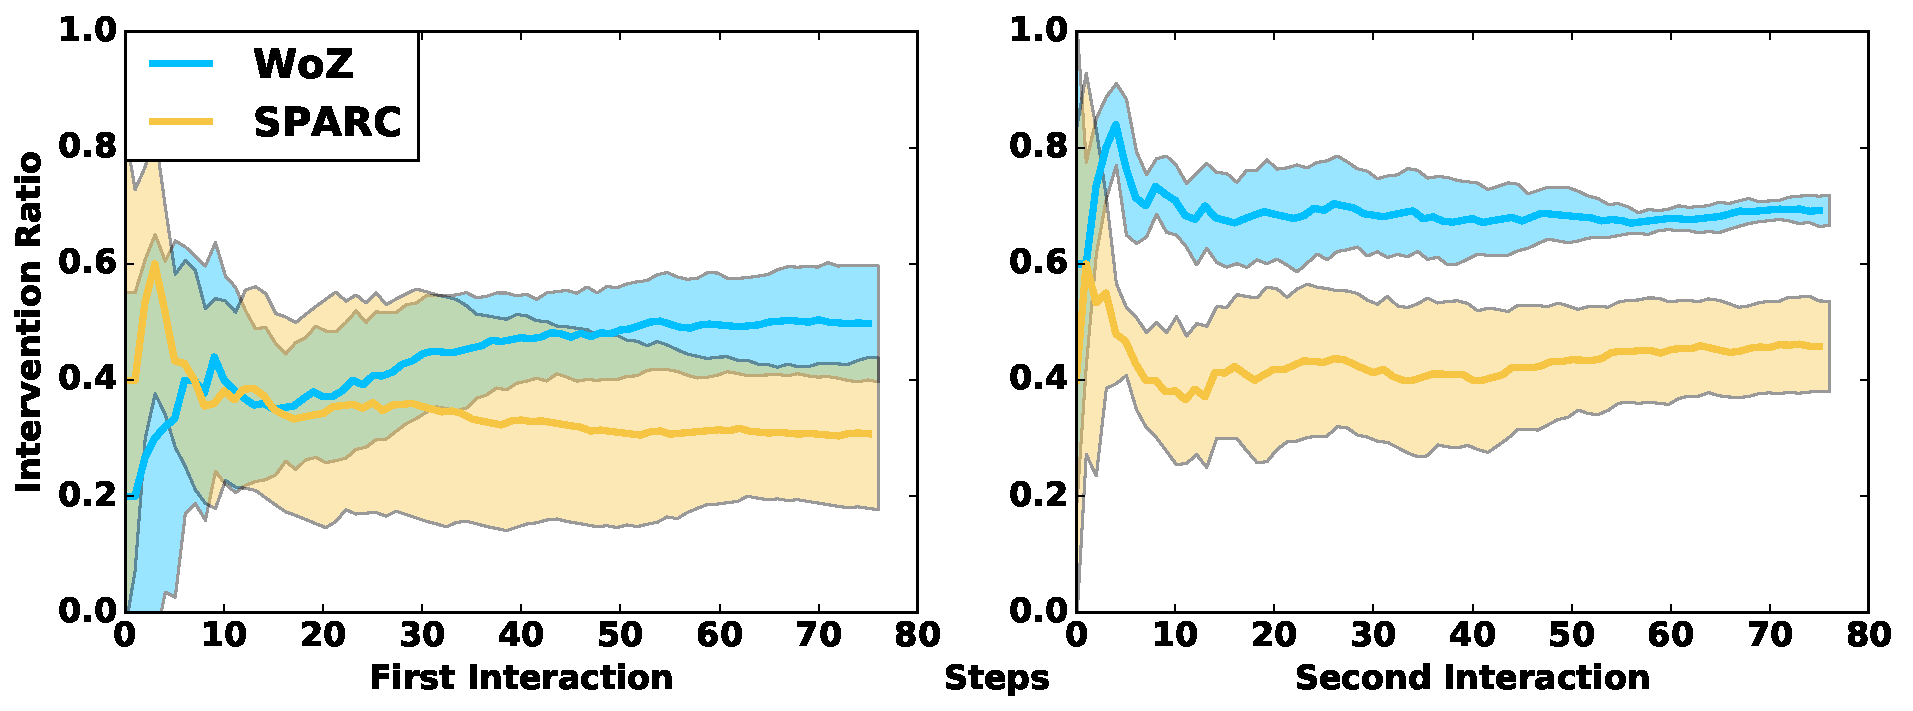
\includegraphics[width=1.\textwidth]{ratio_time.pdf}
	\caption{Evolution of intervention ratio over time for both conditions and both orders. Shaded area represents the 95\% CI (N=5 for each plot).}
	\label{fig:woz_ratio_time}
\end{figure}

For both the performance and the intervention ratio, a strong ordering effect was observed. Figure~\ref{fig:woz_separated} and Table~\ref{tab:woz_comp_means} present the performance and final intervention ratio separated by condition and order. In both orders, the performance in the second interaction was higher than the one in the first interaction, as the participants were used to the system and developed an efficient interaction policy. On the other hand, the performance between condition for the same interaction number was similar (in both their first and second interactions, the condition of interaction did not impact the performance). However, for both orders, when comparing between condition for the same interaction number, the intervention ratio was lower when using \gls{sparc} compared to \gls{woz}. This indicates that when the wizarded-robot learned using \gls{sparc}, a similar performance was attained as with \gls{woz}, but the number of interventions required to achieve this performance was lower.

%COuld use the CIDM if desired or not

\begin{figure}[ht]
	\centering
	\begin{subfigure}[t]{0.5\textwidth}
		\centering
		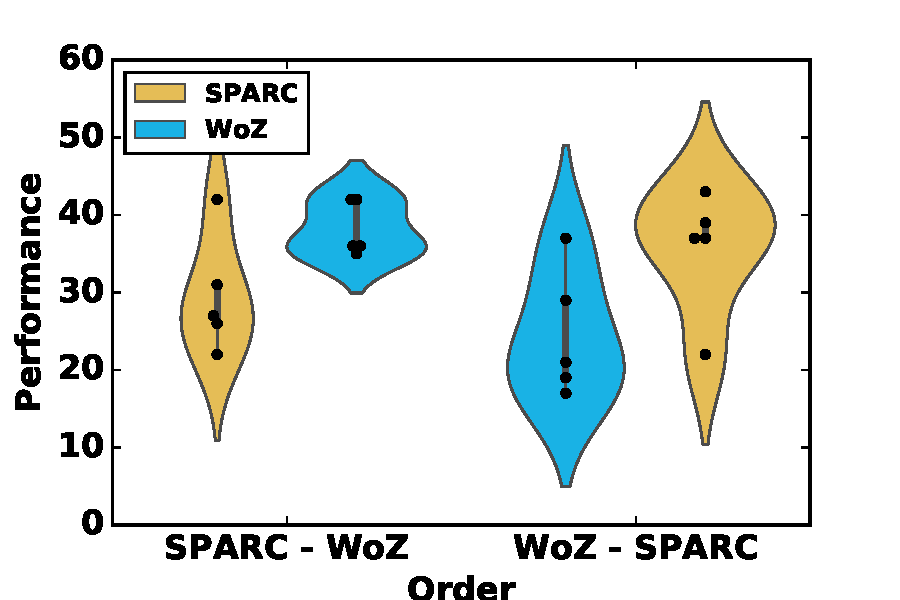
\includegraphics[width=1.\textwidth]{perf_divided.pdf}
	\end{subfigure}%
	\begin{subfigure}[t]{0.5\textwidth}
		\centering
		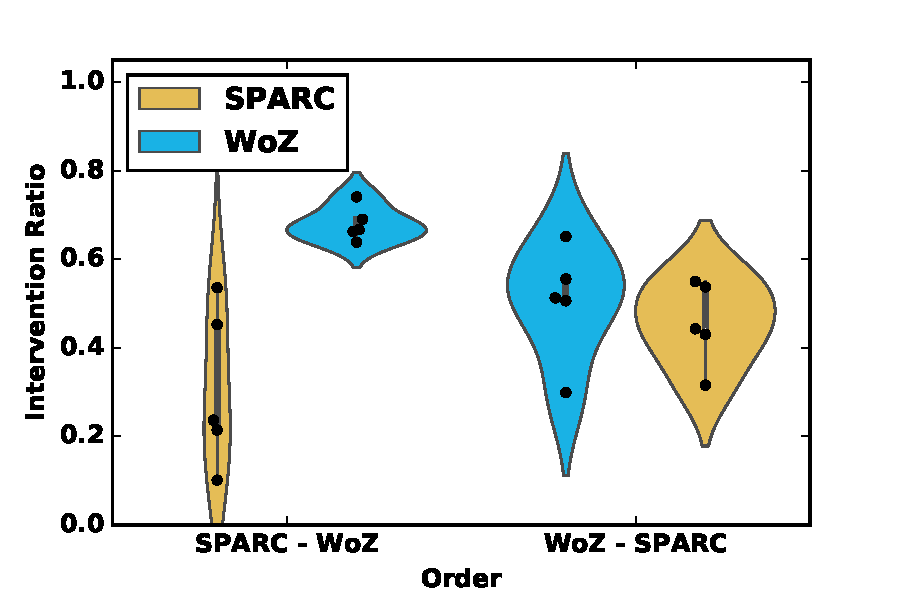
\includegraphics[width=1.\textwidth]{ratio_divided.pdf}
	\end{subfigure}
	\caption{Performance achieved and final intervention ratio separated by order and condition. For each order, the left part presents the metric in the first interaction (with one condition) and the right part the performance in the second interaction (with the other condition).}
	\label{fig:woz_separated}
\end{figure}


\begin{table}[t]
	\caption{Average performance and intervention ratio separated by condition and order.}
	\centering
	\ra{1.2}
\begin{tabular}{@{}lllcll@{}}\toprule
	& \multicolumn{2}{c}{Order S-W} & \phantom{abc} & \multicolumn{2}{c}{Order W-S} \\
	\cmidrule{2-3} \cmidrule{5-6}
	& SPARC & WoZ && WoZ & SPARC \\
	& (int 1) & (int 2) && (int 1) & (int 2) \\
	\midrule			
Performance M & 29.6 & 38.2 && 24.6 & 35.6 \\
95\% CI & [23.6,35.6] & [35.5,40.9] && [18.1,31.1] & [29.3,41.9]\\[.2cm]
Intervention Ratio M & 0.31 & 0.68 && 0.5 & 0.46 \\
95\% CI & [0.17,0.45] & [0.65,0.71] && [0.4,0.61] & [0.38,0.53]\\
\bottomrule
\end{tabular}
\label{tab:woz_comp_means}
\end{table}

%In both conditions, the average performance in the second interaction (\textit{M$_{S-W-2}$} =38, 95\% CI [36.2, 39.8], \textit{M$_{W-S-2}$}=34.8, 95\% CI [30.8, 38.8]) was higher than in the first one (\textit{M$_{S-W-1}$}=29.4, 95\% CI [25.3, 33.5], \textit{M$_{W-S-1}$}=24.3, 95\% CI [19.4, 29.4]; Fig.~\ref{fig:graphs} \textit{left}). The 95\% \textit{Confidence Interval of the Difference of the Mean} (CIDM) for the L-W-S condition is [4.1, 13.1] and for the W-S-L condition is [4.0, 16.8].
%However, the performance is similar when only the interaction order (first or second) is considered. 
%The participants performed slightly better in the S-W condition, but the CIDM includes zero in both cases (95\% CIDM$_{1}$ [-1.5, 11.5], 95\% CIDM$_{2}$ [-1.2, 7.6]). 
%In the condition L-W-S, the intervention ratio increased between the learning and non learning condition (\textit{M$_{S-W-1}$}=0.31, 95\% CI [0.20, 0.42] to \textit{M$_{S-W-2}$}=0.68, 95\% CI [0.66, 0.70], CIDM$_{S-W}$=[0.26, 0.48]). 
%But in the W-S condition, the intervention ratio is almost identical between the two interactions but slightly lower for the learning case (\textit{M$_{W-S-1}$}=0.50, 95\% CI [0.44, 0.57] to \textit{M$_{W-S-2}$}=0.46, 95\% CI [0.40, 0.51], CIDM$_{W-S}$ [-0.03, 0.13]).

Additionally, a strong positive correlation (Pearson's \textit{r}=0.79) was found between the average child-robot motivation and engagement and its performance which shows that the performance achieved by the child-robot represented the capacity of the teacher to keep both engagement and motivation high.

\subsection{Questionnaire Data}

The post-interaction questionnaires evaluated the participant's perception of the child-robot's learning and performance, the quality of suggestions made by the wizarded-robot, and the experienced workload. All responses used seven point Likert scales. Table~\ref{tab:woz_quest_means} presents separated results for the questions asked in the post-interaction questionnaires, with more details for the questions exhibiting differences in Figure~\ref{fig:woz_quest}.

\begin{figure}[ht]
	\centering
	\begin{subfigure}[t]{0.3295\textwidth}
		\centering
		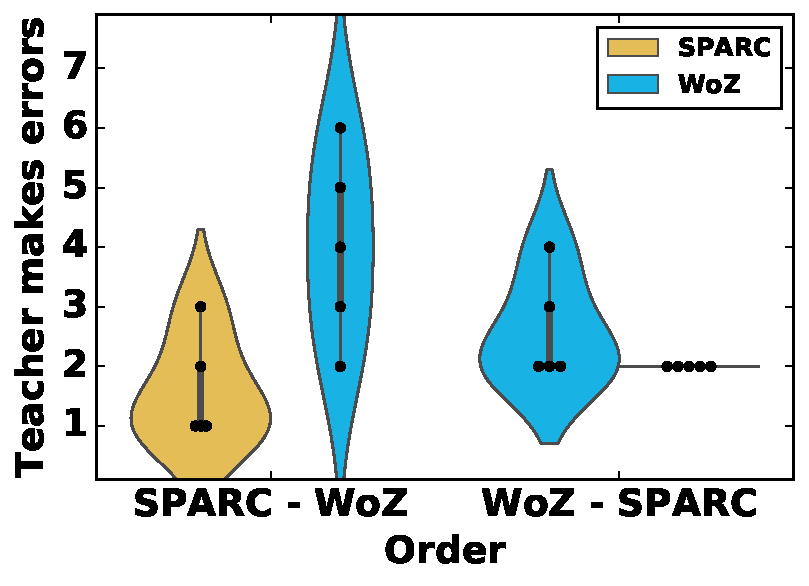
\includegraphics[width=1.\textwidth]{errors.pdf}
	\end{subfigure}%
	~ 
	\begin{subfigure}[t]{0.341\textwidth}
		\centering
		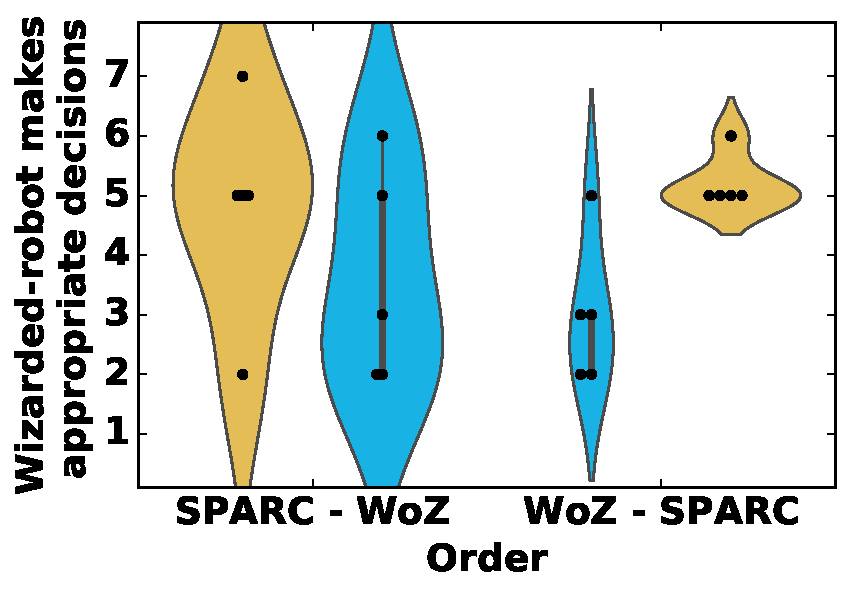
\includegraphics[width=1.\textwidth]{appropriate.pdf}
	\end{subfigure}%
	~ 
	\begin{subfigure}[t]{0.3295\textwidth}
		\centering
		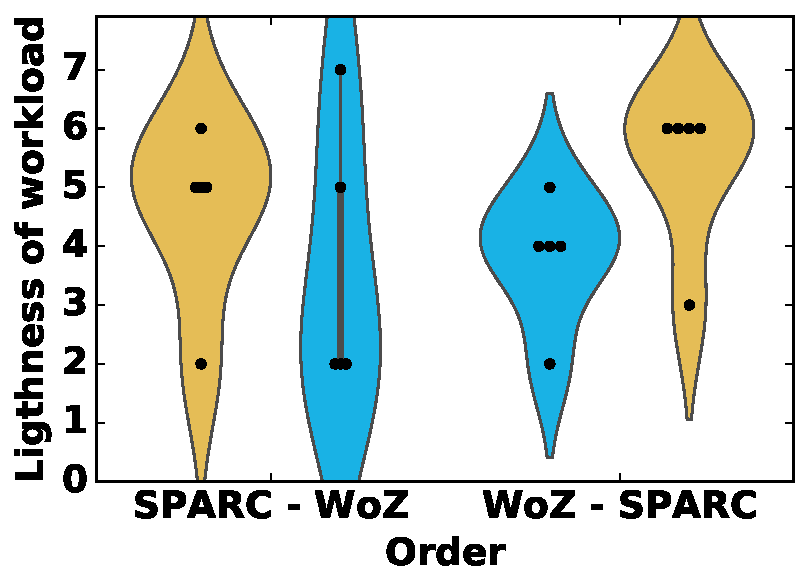
\includegraphics[width=1.\textwidth]{workload.pdf}
	\end{subfigure}
	\caption{Questionnaires results on robot making errors, making appropriate decisions and on lightness of workload.}
	\label{fig:woz_quest}
\end{figure}

Across the four possible interactions, the rating of the child-robot's learning was similar (\textit{M}=5.25, 95\% CI [4.8, 5.7]). As the child-robot was using the same interaction model in all four conditions, this result is expected. There is a slight tendency to rate the child's performance as being higher in the \gls{woz} condition but the error margin is too high to conclude anything. %This could indicate that the teachers were more aware of the child's behaviour as the workload was lighter to control the wizarded-robot.

\begin{table}[t]
	\caption{Average reporting on questionnaires separated by condition and order.}
	\centering
	\ra{1.2}
\begin{tabular}{@{}lllcll@{}}\toprule
	& \multicolumn{2}{c}{Order S-W} & \phantom{abc} & \multicolumn{2}{c}{Order W-S} \\
	\cmidrule{2-3} \cmidrule{5-6}
	& SPARC & WoZ && WoZ & SPARC \\
	& (int 1) & (int 2) && (int 1) & (int 2) \\
	\midrule					
		Child learns M & 5.2 & 5.2 && 5.2 & 5.4 \\
		95\% CI & [3.7,6.7] & [3.8,6.6] &&  [4.2,6.2] & 4.7,6.1]\\[.2cm]
		Child's performance M & 4.6 & 5.0 && 5.0 & 4.4 \\
		95\% CI & [3.4,5.8] & [3.3,6.8] && [4.0,6.0] & [3.7,5.1]\\[.2cm]
		Wizarded-robot makes errors M & 1.6 & 4.0 && 2.6 & 2.0 \\
		95\% CI & [0.9,2.3] & [2.8,5.2] && [1.9,3.3] & [2.0,2.0] \\[.2cm]
		Wizarded-robot makes appropriate & 4.8 & 3.6 && 3.0  & 5.2 \\
		decisions M 95\% CI & [3.4,6.2] & [2.2,5.0] && [2.0,4.0] & [4.9,5.6] \\ [.2cm]
		Lightness of workload M & 4.6  & 3.6 && 3.8  & 5.4 \\
		95\% CI & [3.4,5.8] & [1.8,5.4] && [2.9,4.7] & [4.4,6.5] \\
		\bottomrule
	\end{tabular}
	\label{tab:woz_quest_means}
\end{table}


Participants rated the wizarded-robot as more suited to operate unsupervised with \gls{sparc} than with \gls{woz}  (\gls{cidm} for S-W ordering [-0.2, 2.6], \gls{cidm} for the W-S ordering [1.6, 2.8]).

Similarly, a trend was found showing that the wizarded-robot with \gls{sparc} is perceived as making fewer errors than with \gls{woz} (\gls{cidm} for S-W ordering [1.3, 3.4], \gls{cidm} for the W-S ordering [0.1, 1.1]). 

Also participants tended to rate the workload as lighter when interacting with \gls{sparc}, and this effect is much more prominent when the participants interacted with the \gls{woz} first (\gls{cidm} for S-W ordering [-0.6, 2.6], \gls{cidm} for the W-S ordering [0.7, 2.5]).

Most of the difference of mean interval exclude 0 or include it marginally, which would indicate tendency of difference, but due to the low number of participants, no statistical tests are applicable and as such no significance can be demonstrated. 

%SHould I present results from the post experiment questionnaire, and/or going more in details on the results

\section{Discussion}

Strong support for H1 (a good teacher leads to a better child performance) was found, a correlation between the average value of states (engagement and motivation) and the final performance for all of the 10 participants was observed (\textit{r}=0.79). This validity check confirms that the performance of the child robot reflects the performance of the teacher in this task: supervising the wizarded-robot to execute an efficient action policy maximising the inner state of the child-robot. Additionally, the model of the child robot exhibited the desired behaviour: allowing a wide range of performances without one obvious optimal action policy.

The results also provided support for H2 (teachers create personal strategies): all the participants performed better in the second interaction than in the first one. This suggests that participants developed a strategy when interacting with the system in the first interaction, and were able to use it to increase their performance in the second interaction. Looking in more detail at the interaction logs, different strategies for the wizarded-robot can be observed. For instance, the ratio of waiting action compared to other supportive actions varied between participants (from 4.7\% to 56\%). This variation demonstrates that despite the repeatability of the environment, different participants applied different strategies when controlling and teaching a robot.

H3 (reducing the number of interventions reduces the perceived workload) is partially supported: the results show a trend for participants to rate the workload as lighter when interacting with the \gls{sparc}, and another trend between using \gls{sparc} and the intervention ratio. However, when computing the correlation between the intervention ratio and the reported workload, a strong effect can only be observed in the second interaction ($\rho = -.622$). In the first interaction, the main cause of the workload is probably the discovery of the system and how to interact with it rather than the requirement to manually select actions for the robot. Nevertheless, regardless of the order of the interactions, \gls{sparc} tended to receive higher ratings for lightness of workload and required fewer interventions to be controlled which indicates that using \gls{sparc} could decrease workload on robot's supervisor compared to \gls{woz}.

Finally, H4 (using learning maintains similar performance, but decreases the workload) is supported: interacting with a learning robot in the \gls{sparc} condition resulted in a similar performance than interacting with a non-learning robot in the \gls{woz} condition, whilst requiring fewer active interventions from the supervisor and a lower workload to control. Reducing the workload on the robot operator has real world utility, for example, in the context of \gls{rat}, it might free time for the supervisor to allow them to focus on other aspects of the intervention, such as analysing the child's behaviour rather than solely controlling the robot. 

It should be noted that the actual learning algorithm used in this study is only of incidental importance, and that certain features of the supervisor's strategies may be better approximated with alternative methods -- of importance for the present work is the presence of learning at all. Other algorithms and ways to handle time have been used in the following studies presented in Chapters~\ref{chap:control} and~\ref{chap:tutoring}.

\section{Summary}
%\ES{relation with RQ}
%As expected, using \gls{sparc} to teach a robot to interact under supervision did allow the robot to partially learn an interaction policy which decreases the requirement on the teacher to physically enforce each robot's actions. Additionally, \gls{sparc} decreased also the workload imposed on the robot supervisors which has real world impact as today many subfields of \gls{hri} such as \gls{rat} still rely on \gls{woz} for their robotic control.

Using a suggestion/intervention system, \gls{sparc} allowed online learning for interactive scenarios, thus increasing autonomy and reducing the demands on the supervisor. Results showed that the learning component of \gls{sparc} allowed participants to achieve a similar performance as interacting with a non-learning robot, but requiring fewer interventions to attain this result. This suggests that while both conditions allowed the participants to reach a good performance, with \gls{sparc}, the presence of learning shifts part of the burden of selecting actions onto the wizarded-robot rather than on the human. Using \gls{sparc}, the robot partially learnt an interaction policy which decreased the requirement on the teacher to physically enforce each robot's actions. This indicates that a learning robot could reduce the workload on the operator freeing them to do more valuable tasks and that \gls{sparc} could be an efficient interaction framework to operate this learning. In addition to providing a robot with autonomy, this reduction of workload has real world implications, in the context of \gls{rat}, it could allow the therapist to focus more on the child than on the robot, with improved therapeutic outcomes as potential result. 


\cleartooddpage

\chapter[Study 2: Importance of Control Over the Learner]{Study 2: \\ Importance of Control Over the Learner}\label{chap:control}
\glsresetall
\graphicspath{{images/control/}}

\newcommand{\nosemic}{\SetEndCharOfAlgoLine{\relax}}% Drop semi-colon ;
\newcommand{\dosemic}{\SetEndCharOfAlgoLine{\string;}}% Reinstate
\newcommand{\pushline}{\Indp}% Indent
\newcommand{\popline}{\Indm\dosemic}% Undent

\begin{framed}
	\textbf{Key points:}
	
	\begin{itemize}
		\item Design of an experiment comparing \acrshort{sparc} and another \acrshort{iml} method: \acrshort{irl}.
		\item The application domain is a replication of the world used in early studies evaluating \acrshort{irl}.
		\item \acrshort{irl} uses partial guidance to the robot and explicit rewarding of the robot's action to teach it a policy.
		\item \acrshort{sparc} uses full control over the robot's action, implicit rewards and evaluation of intentions rather than actions.
%		\item \acrshort{sparc} was combined with \acrlong{rl}.
		\item Results from a mixed design study involving 40 naive participants show that \acrshort{sparc} achieves a better performance and an easier and faster teaching than \acrshort{irl}.
	\end{itemize}
\end{framed}

Parts of the work presented in this chapter have been published verbatim in \cite{senft2017supervised} \footnote{Note about technical contribution in this chapter: the author reimplemented every part of the system using Qt.}. The final publication is available from Elsevier via
\begin{itemize}
	\item \url{https://doi.org/10.1016/j.patrec.2017.03.015}.
\end{itemize} 

\newpage
\section{Motivation}

Previous work in \gls{iml} showed that humans want to teach robots not only with feedback on their actions but also by communicating the robots what they should do \citep{thomaz2008teachable,amershi2014power}. However, in most research where agents are taught policies using human guidance, the teacher is given little or no control over the agent's actions and has to observe the agent executing an action even when knowing that this action is incorrect (cf. Section \ref{ssec:back_feedback}). This chapter explores how these \gls{iml} approaches could be improved by applying the principles of the \gls{sparc} defined in Chapter \ref{chap:sparc}. This chapter also presents experimental results demonstrating how these principles influence the learning process, the agent performance and the user experience and how these results compare to other traditional \gls{iml} approaches.

The study presented in Chapter \ref{chap:woz} explored how \gls{sparc} could be used with \acrlong{sl}, to replicate a teacher's action policy. However, some of the most promising features of \gls{iml} arise when combined with \gls{rl} as it might allow an agent to learn beyond the demonstrations \citep{abbeel2004apprenticeship}. As such, this chapter proposes a way to apply the principles underlying \gls{sparc} to classical feedback based \gls{rl} and evaluates how this human control over the robot's actions impacts the learning. This chapter presents results from a study involving 40 participants comparing the teaching efficiency and user experience of \gls{sparc} to \gls{irl}, another \gls{iml} approach offering less control but having been validated in previous studies \citep{thomaz2008teachable}. %The testing environment of \acrshort{irl} has been reimplemented to stay as close as possible to the online version of the task.

\section{Scope of the Study}


\subsection{Interactive Reinforcement Learning}

\gls{irl} implements the principles presented in \cite{thomaz2008teachable}(hereafter the `original study' or `original paper'): a human supervises and teaches an agent to interact autonomously in an environment. This teaching is achieved by providing guidance and positive or negative feedback on the last action executed by a robot. In this study, the algorithm controlling the robot combines this human feedback with environmental ones to form a reward used to update a Q-table. This Q-table assign a Q-value (interest of taking an action) to every state-action pair and is used to select the next action. Three additions to the standard interaction mechanism have been proposed and implemented by Thomaz and Breazeal and are used in this study as well: guidance, communication by the robot and an undo mechanism \citep{thomaz2008teachable}. 

The guidance channel emerged from the results of a pilot study where participants assigned rewards to objects to indicate that the robot should do something with them. With the guidance channel, teachers can direct the attention of the robot toward certain items in the environment, informing the robot that it should use them in its next action. This guidance behaviour offers partial control over the robot's actions restricting the executable options, but cannot be used to explicitly set the robot's behaviour. 

Additionally, the robot communicates uncertainty by directing its gaze toward different parts of the environment with equally high probability of being used next. The aim of this communication of uncertainty is to provide transparency about the robot's internal state, for example indicating when the robot is unsure about its next action and that guidance should be provided. 

Finally, the undo mechanism aims to provide a way for the teacher `cancel' the robot's action, to bring it back to relevant part of the world after an error, in order to speed up the teaching. After receiving a negative reward, the robot tries to cancel the effect of the previous action on the environment (if possible), resulting in an undo behaviour. As shown in the original studies, these three additions improve the robot's performance on the task and the user experience.

In summary, Teachers have two ways to transmit information to the robot: a reward channel (providing a numerical evaluation of the last action) and a guidance channel (directing the robot's attention toward parts of the state to restrict the exploration).

\subsection{SPARC}

\gls{sparc} uses a single type of input from the human similar to the guidance in \gls{irl} and no reward channel. However with \gls{sparc}, the guidance channel directly controls the actions of the robot. On the other hand, the robot communicates all of its intentions (i.e the action it plans to execute next) to its teacher by looking at the corresponding part of the environment. Following the principles proposed in Section \ref{sec:sparc_principles}, the teacher can either not intervene, letting the robot execute the suggested action or step in and force the robot to execute an alternative action. This combination of suggestions and corrections gives the teacher full control over the actions executed by the robot. This also makes the rewards redundant. Rather than requiring the human to explicitly provide rewards, a positive reward is directly assigned to each action executed by the robot as it has been either enforced or passively approved by the teacher.

\subsection{Differences Between IRL and SPARC}

Unlike \gls{irl}, \gls{sparc} offers the user full control over the actions executed by the robot. \gls{sparc} changes the learning paradigm from learning from the human's evaluation of actions' impacts to learning from the human's knowledge and the \emph{expected} impact of actions. An expert in the task domain evaluates the appropriateness of actions before their execution and can guide the robot to act in a safe and useful manner. This implies that the robot does not rely on observing the negative effects of an action to learn to avoid it (as in \gls{irl} or more generally \gls{rl}), but rather it learns what the best action is for each state. Even in a non-deterministic environment such as human-robot interactions, some actions can be expected to have a negative consequence. And the human teacher should be able to stop the robot from ever executing them, preventing the robot from causing harm to itself or its social or physical environment. 

Another noticeable difference is the type of information the robot communicates with the user: in \gls{irl}, the robot communicates its uncertainty about an action and with \gls{sparc} its unambiguous intention to execute an action. Similarly, the communication from the user to the  robot differs between the two approaches. In \gls{sparc} the user can offer the whole action space as commands to the robot, which removes the need for explicit rewards, while in \gls{irl}, the teacher can guide the robot toward a subset of the action space and has to manually provide feedback to evaluate the robot's decisions. A result is that the quantity of information provided by the user to the robot is similar for both \gls{irl} and \gls{sparc}. 

\subsection{Hypotheses}

Three hypotheses have been tested in the study:

\begin{enumerate}
	\item [H1] \textit{Effectiveness and efficiency with non-experts.} \gls{irl} and \gls{sparc} will have differences in performance, speed, number of inputs used, mental effort on the teacher and the number of errors during the teaching phase when used by non-experts. We predict that for each metric, \gls{sparc} will lead to better results. \ES{could probably rephrase to keep style consistent}
	\item [H2] \textit{Safety with experts.} \gls{sparc} can be used by expert users (knowledgeable in the interaction process) to teach an action policy safely, quickly and efficiently, achieving better results than other \gls{iml} methods lacking control.
	\item [H3] \textit{Control.} Teachers prefer a method in which they can have more control over the robot's actions.
\end{enumerate}
\section{Methodology}
\subsection{Participants}

A total of 40 participants (age \textit{M}=25.6, \textit{SD}=10.09; 24F/16M) were recruited using a tool provided by the University of Plymouth to reach a mixed population of students and non-student members of the local community\footnote{\url{https://uopsop.sona-systems.com/Default.aspx?ReturnUrl=\%2f}}. At the start of the experiment, all participants gave written informed consent, were told of the option to withdraw at any point and completed a demographic questionnaire. Participants were mostly not knowledgeable in machine learning and robotics (familiarity with machine learning \textit{M}=1.8, \textit{SD}=1.14; familiarity with social robots \textit{M}=1.45, \textit{SD}=0.75 - Likert scale ranging from 1: not at all familiar to 5: extremely familiar). The study lasted around one hour and followed a 2x2x3 mixed design where participants interacted with both conditions three times. To avoid ordering effects, the order of interaction was counterbalanced between two groups: group 1 interacting with \gls{irl} then \gls{sparc} and the interaction order is inverted for group 2 (see also Figure \ref{fig:control_design}). Participants were distributed randomly between the two groups whilst balancing gender and age. All participants received remuneration at the standard U.K. living wage rate, pro rata. 

In addition to naive non-expert users, an expert user (the author) interacted five times with each system following a strictly optimal strategy for both conditions. These results from the expert are used to evaluate H2 and show the optimal characteristics of each system (\gls{irl} and \gls{sparc}) when used by trained experts in robot interaction, such as therapists in the context of assistive robotics.


\subsection{Task} \label{ssec:control_task}

The task used in this study is the same as \cite{thomaz2008teachable}: ``Sophie's kitchen'', a simulated environment presented on a computer where a virtual robot has to learn how to bake a cake in a kitchen. As the source code was not available, the task was reimplemented to stay as close as possible to the description in the paper and the online version of the task\footnote{\url{http://www.cc.gatech.edu/~athomaz/sophie/WebsiteDeployment/}}.

The scenario is the following: a robot, Sophie, is in a kitchen with three different locations (shelf, table and oven) and five objects (flour, tray, eggs, spoon and bowl) (see Figure \ref{fig:control_initial}). The participant has to teach Sophie to bake a cake by guiding it through a sequence of steps while giving enough feedback so the robot learns a correct series of actions leading to the completion of the task. There are six crucial steps to achieve a successful result:

\begin{enumerate}
	\item Put the bowl on the table (Figure \ref{fig:control_bowl}).
	\item Add one ingredient to the bowl (flour or eggs).
	\item Add the second ingredient (Figure \ref{fig:control_ingredients}).
	\item Mix the ingredients with the spoon to obtain batter (Figure \ref{fig:control_batter}).
	\item Pour the batter in the tray (Figure \ref{fig:control_tray}).
	\item Put the tray in the oven (Figure \ref{fig:control_goal}).
\end{enumerate}

The environment is a deterministic \gls{mdp}, defined by a state, a set of actions (move left, move right, pick up, drop and use), a deterministic transition function and an environmental reward function. The environment includes end states, corresponding to a success or a failure, which reset the simulation to the initial state and provide a reward (+1 for success and -1 for failure). All the other states corresponding to intermediate steps have a reward of -0.04 to penalise long sequences. Different action policies can lead to success, but many actions end in a failure state, for example putting the spoon in the oven. This environment includes a large number of possible states (more than 10,000), success and failure states and a sparse environmental reward function. These elements increase the value of having a teacher present to support the learning. As argued by Thomaz and Breazeal in the original paper, this environment provides a good setup to evaluate methods of teaching a robot.

\begin{figure}[ht]
	\centering
	\begin{subfigure}[b]{0.325\textwidth}
		\centering
		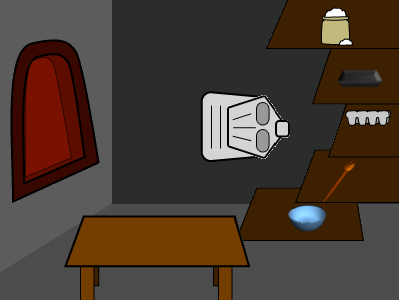
\includegraphics[width=\textwidth]{step0.png}
		\caption{Initial state}
		\label{fig:control_initial}
	\end{subfigure}
	\centering
	\begin{subfigure}[b]{0.325\textwidth}
		\centering
		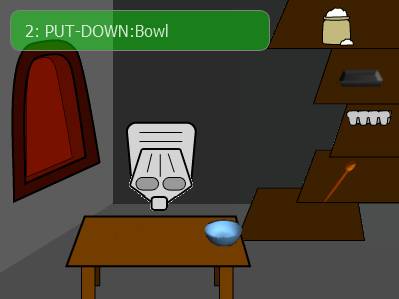
\includegraphics[width=\textwidth]{step1.png}
		\caption{Step 1}
		\label{fig:control_bowl}
	\end{subfigure}
	\centering
	\begin{subfigure}[b]{0.325\textwidth}
		\centering
		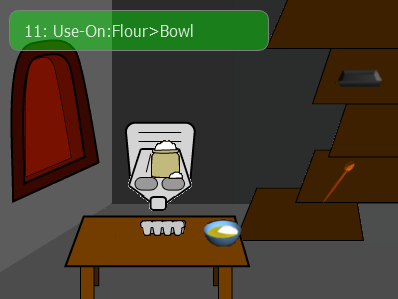
\includegraphics[width=\textwidth]{step3.png}
		\caption{Step 3}
		\label{fig:control_ingredients}
	\end{subfigure}
	
	
	\centering
	\begin{subfigure}[b]{0.325\textwidth}
		\centering
		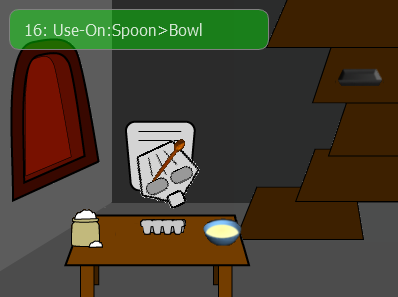
\includegraphics[width=\textwidth]{step4.png}
		\caption{Step 4}
		\label{fig:control_batter}
	\end{subfigure}
	\centering
	\begin{subfigure}[b]{0.325\textwidth}
		\centering
		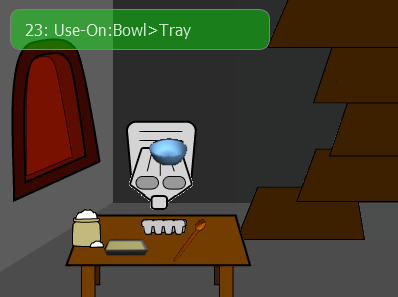
\includegraphics[width=\textwidth]{step5.png}
		\caption{Step 5}
		\label{fig:control_tray}
	\end{subfigure}
	\centering
	\begin{subfigure}[b]{0.325\textwidth}
		\centering
		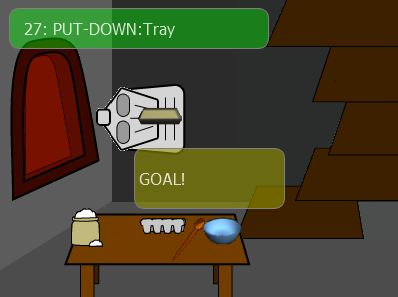
\includegraphics[width=\textwidth]{step6.png}
		\caption{Step 6}
		\label{fig:control_goal}
	\end{subfigure}
	
	\caption{Presentation of different steps in the environment. (a) initial state, (b) step 1: bowl on the table, (c) step 3: both ingredients in the bowl, (d) step 4: ingredients mixed to obtain batter, (e) step 5: batter poured in the tray and (f) step 6 (success): tray with batter put in the oven. (Step 2: one ingredient in the bowl has been omitted for clarity, two different ingredient could be put in the bowl to reach this state)}
	\label{fig:control_states}
\end{figure}

\subsection{Implementation}

Two conditions were constructed to compare the \gls{irl} and \gls{sparc} approaches to this task. The underlying learning mechanism is identical in both conditions. The only differences lie in the manner of interaction (inputs to and from the algorithm) and the amount of control over the robot's actions. With \gls{irl} teachers have to explicitly provide rewards and have a partial control over the action selection, while with \gls{sparc} rewards are implicit and the control over actions is total. 

The learning algorithm (see Algorithm \ref{algo:control_sparc} and \ref{algo:control_irl}) is a variation on Q-learning, without reward propagation\footnote{In Q learning the update function is $Q(s_{t},a_{t}) \leftarrow Q(s_{t},a_{t}) + \alpha (r_{t}+\gamma (\underset{a}{max} Q(s_{t+1},a))-Q(s_{t},a_{t}))$}. This guarantees that any learning by the robot is due to the human's teaching, and as such provides a lower bound for the robot's performance. %By using Q-learning, the robot's testing performance would be higher. 
Similarly to the original study, the algorithm uses a learning rate $\alpha = 0.3$ and a discount factor $\gamma = 0.75$.

\begin{table}
\caption{Simplified outline of algorithms used for both condition.}
		
\begin{minipage}[t]{0.5\textwidth}
	\vspace{0pt}  
	\begin{algorithm}[H]
		
		\caption{SPARC}
		\label{algo:control_sparc}
		\begin{minipage}{0.9\linewidth}
		\hspace{-20pt} 
			\While{learning}{
			 	$a_{t}$ = $ arg \underset{a}{max} Q[s_{t},a]$
			 	
			 	look at object or location used in $a_{t}$
			 
			 	
			 	\While{waiting for command (2 seconds)}{
			 		\eIf{received command}{
			 			$a_{t}$ = received command
			 			
			 			$r_{t} = 0.5$
			 		}{
			 		$r_{t} = 0.25$
			 	}
			 }
			 \vspace{29.75pt}
			 \nosemic Act in the world:\;
			 \pushline\dosemic execute $a_{t}$, transition to $s_{t+1}$
			 
			 \popline $r_{t} = r_{t} + r_{environment}$
			 
			 \nosemic Learn:
			 
			 \pushline\dosemic $Q(s_{t},a_{t}) \leftarrow Q(s_{t},a_{t}) + \alpha (r_{t}+\gamma (\underset{a}{max} Q(s_{t},a))-Q(s_{t},a_{t}))$
			}
		\end{minipage}
	\end{algorithm}
\end{minipage}%
\begin{minipage}[t]{0.5\textwidth}
	\vspace{0pt}
	\begin{algorithm}[H]
		\caption{IRL
			\vspace{0.05pt}}
		\label{algo:control_irl}
		
		\begin{minipage}{0.9\linewidth}
			\hspace{-20pt} \While{learning}{
			$A_{t+1}=[a^{1}...a^n]$, $n$ actions with high $Q[s_{t+1},a^{i}]$
					
%			\vspace{5.5pt}
			
			\While{waiting for guidance and reward on $a_{t}$ (2 seconds)}{
				\If{$n>1$}{
					indicate confusion 
				}
				\If{received reward $r_{t}'$}{
					$r_{t} = r_{t} + r_{t}'$				
				}
				\If{receiving guidance}{
					\If{guidance acceptable}{
						$a_{t+1}$ = guidance
					}
				}
		}
		
		\nosemic Learn:
		 
		\pushline\dosemic$Q(s_{t},a_{t}) \leftarrow Q(s_{t},a_{t}) + \alpha (r_{t}+\gamma (\underset{a}{max} Q(s_{t},a))-Q(s_{t},a_{t}))$
		
		\popline \nosemic Act in the world:
		
		\pushline\dosemic execute $a_{t+1}$, transition to $s_{t+2}$
		
		\popline$r_{t+1} = r_{environment}$
	}
	\end{minipage}
	\end{algorithm}
\end{minipage}
\label{tab:control_algo}
\end{table}

As shown in Table \ref{tab:control_algo}, another difference between the conditions is that with \gls{sparc}, the algorithm learns immediately after executing an action (and only with positive rewards). On the other hand, \gls{irl} learns about an action just before executing the next one, based on a positive or negative evaluation received between the actions.

\subsubsection{Interactive Reinforcement Learning}

We have implemented \gls{irl} following the principles presented in \cite{thomaz2008teachable}. The user can use the left mouse-click to display a slider providing rewards. Guidance is implemented by right-clicking on objects to direct the robot's attention toward a specific object. Guidance can only be provided for objects the robot is facing, otherwise right-clicking has no effect. Following a guidance message, the robot will execute the candidate action involving the object. The action space is not entirely covered by this guidance mechanism: for example, it does not cover moving from one location to another. This guidance gives a partial opportunity to the user to limit the exploration for the current step, without preventing the robot to explore in further steps.

Some modifications to the original study were required due to the lack of implementation details in the original paper, one of them being the use of a purely greedy policy instead of using softmax. As, the presence of human rewards and guidance limits the importance of autonomous exploration, the greediness of the algorithm should assist the learning by preventing the robot from exploring outside of the guided policy. 

It should be noted that the presence of the human in the learning process alters deeply the concept of convergence. By providing rewards, the teacher can manually force the robot's policy to converge or diverge.

\subsubsection{SPARC}

\gls{sparc} uses the gaze of the robot toward objects or locations to indicate to the teacher which action the robot is suggesting. Similarly to the guidance in \gls{irl}, the teacher can use the right click of the mouse on objects to send a `command' to the robot and have it execute the action associated to this object in the current state. However, in this condition, this communication has been extended to also cover locations. With \gls{sparc}, the command covers the whole action space: at every time step, the teacher can specify, if desired, the next action to be executed by the robot. Similarly to the guidance, this command can be used on objects only if the robot is facing them. If a robot's suggested action is not corrected, a positive reward of 0.25 is automatically received (as it has the implicit approval from the teacher). If the teacher selects another action, a reward of 0.5 is given to the selected action (the corrected action is not rewarded). That way, actions actively selected are more reinforced than the ones accepted passively and participants still have access to a wider range of rewards with \gls{irl}. This system allows for the use of reinforcement learning with implicit reward assignation, aiming to simplify the teaching interaction.

\subsection{Interaction Protocol}

Participants were divided into two groups and interacted with both \gls{irl} and \gls{sparc}, with the order of presentation being counterbalanced between groups (see Figure \ref{fig:control_design}). Participants in group 1 interacted with \gls{irl} first for three sessions and then with \gls{sparc} for the three remaining sessions; and the interaction order was inverted for participants in group 2. 

\begin{figure}[ht]
	\centering
	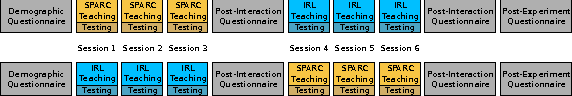
\includegraphics[width=1\textwidth]{protocol.pdf}
	\caption{A representation of the timeline experienced by participants according to the order they were in. The top row corresponds to group 1 and bottom row to group 2.}
	\label{fig:control_design}
\end{figure}

After welcoming participants and before interacting with a system, participants completed a demographic questionnaire and received two information sheets. The first one explained the task (describing the environment and how to bake the cake) and the second one described the system they would interact with (\gls{irl} or \gls{sparc}). 

After reading the sheets, participants interacted for three sessions with the system they were assigned to. Each session started with a teaching phase where the participants could interact with the robot to teach it to complete the task. This teaching phase was composed of a number of episodes, corresponding each to a trajectory from the initial state to an end state (success or failure) after which the environment was returned to the initial state. Similarly to the experiment by Thomaz and Breazeal, participants could decide to terminate the teaching phase whenever they desired by clicking on a button labelled `Sophie is ready'. But the teaching phase was automatically terminated after 25 minutes to impose an upper time-limit on the study. 

After the teaching phase, the robot ran a testing phase where the participant's inputs, other than a force stop, were disabled. The test stopped as soon as an ending state was reached or the participant forced a stop (e.g. if an infinite loop occurs). This testing phase aimed to evaluate the participants' performance in the teaching task. The interaction with each system involved three repeated independent sessions with their own teaching and testing phases. This way, we can observe how the interactions evolved as participants got used to interact with a system.

After participants completed their three sessions with the first system, they were asked to complete a first post-interaction questionnaire. Then they received the information sheet for the second system, interacted with it for three sessions and completed a second post-interaction questionnaire.

At the end of the experiment, participants completed a last questionnaire, the post-experiment questionnaire, received the financial compensation and were explained the goal of the study. All information sheets and questionnaires can be found online \footnote{\url{https://emmanuel-senft.github.io/experiment-irl.html}} and the questionnaires are described in Section \ref{ssec:control_questionnaires}.

\subsection{Metrics}

\subsubsection{Interaction Metrics}

We collected four metrics during the teaching phase (teaching performance, teaching time, number of failures and number of inputs provided) and one during the testing phase (the testing performance). All interaction metrics were collected three times per conditions, once for each session. As not all participants reached a success during the testing phases, we used the six key steps defined in Section \ref{ssec:control_task} as a way to evaluate the performance ranging from 0 (no step has been completed) to 6 (the task was successfully completed) during the testing phase. For example a testing where the robot put both ingredients in the bowl but reached a failure state before mixing them would have a performance of 3. 

The testing performance represents the success of participants in teaching the robot to complete the task. On the other hand, the teaching performance corresponds to the highest step reached by participants in the teaching phase and represents a teaching method's ease of guiding the robot. The teaching time is the duration of the teaching phase, ranging from 0 to 25 minutes. The number of failures is the number of times a participant reached a failure state during the teaching phase. It can be related to the risks involved by the teaching; a safe teaching process should lead to a low number of failures, while a risky one would have a high number of failure. The number of inputs corresponds to the number of commands, guidances or feedback inputs used in a teaching session. Similarly to the teaching time, the number of inputs can be seen as the quantity of efforts invested in the teaching process.

\subsubsection{Questionnaires} \label{ssec:control_questionnaires}

The post-interaction and post-experiment questionnaires provided additional introspective information to compare with the quantitative data from the interaction. Two principal metrics were gathered: the workload on participants and the perception of the robot. 

Workload is an important factor when teaching robots. As roboticists, our task is to minimise the workload for the robot's user and to make the interaction as smooth and efficient as possible. Multiple definitions for workload exist and various measures can be found in the literature (e.g. \citealt{wierwille1983evaluation,moray2013mental}). Due to its widespread use in human factors research \citep{hart2006nasa} and clear definition and evaluation criteria, we used the NASA-Task Load Index (TLX) \citep{hart1988development}. Following the methodology proposed to administer NASA-TLX, we averaged the values from all 6 scales (mental, physical and temporal demand, performance, effort and frustration) ranging from 0 (low workload) to 20 (high workload) to obtain a single workload value per participant for each interaction. This assessment was made during the post-interaction questionnaires. This resulted in two measures of workload per participant, one for each condition.

Finally, the participants' perception of the robot was also evaluated in the post-interaction and post-experiment questionnaires using rating questions (measured on a 5 item Likert scale), binary questions (where participants had to select one of the two system), and open questions on the preference of system and the naturalness of the interaction. 

\section{Results}

Most of the results collected in the study were non-normally distributed. Both ceiling and floor effects could be observed depending on the conditions and the metrics. For instance, for the teaching time, some participants preferred to interact much longer than others, resulting in skewed data. Likewise for the testing performance: often participants either reached a successful end state or did not hit any of the sub-goals of the task in the testing phase ending often in two clusters of participants: one at a performance of 6 and one at 0.  Similarly, some participants who interacted a long time with the system did not complete any step, while others could achieve good results in a limited time. Due to the data being not normally distributed and the absence of possible transformation making them normal, Bayesian statistics were conducted using the JASP software \citep{jasp2018}. Three types of test have been used: mixed ANOVA for omnibus comparisons between conditions for the first and the second interaction (between participants), independent t-test for post-hoc comparisons between participants and paired samples t-test for post-hoc comparisons within participants. All tests have been performed using their Bayesian counterpart, which also removed the need for doing a correction on post-hoc tests such as Bonferroni. As such, no p-value is reported, but a B factor representing how much of the variance on the metric is explained by a parameter (if $B < 1/3$ there is no impact, if $B > 3$ the impact is strong, and if $1/3<B<3$ the results are inconclusive; \citealt{jeffreys1998theory,dienes2011bayesian}).

For each interaction metric, two mixed ANOVA between participants were calculated to explore the impact of the conditions on the metric. The first ANOVA was applied to the first interaction (session 1,2 and 3) and compared participants in group 1 interacting with \gls{irl} and participants in group 2 interacting with \gls{sparc}. The second ANOVA was applied on the second interaction (sessions 4, 5 and 6) and compared participants in group 1 interacting with \gls{sparc} and those in group 2 interacting with \gls{irl}. If required, additional post test were made within participants for the three sessions corresponding to each interaction to measure if successive interactions with a same system impacted the metric.

%%Initial results of the first interaction of the participants have been reported in \cite{senft2016providing}.

%\subsection{Interpreting results}

\subsection{Interaction Data}

Five objective metrics (teaching performance, testing performance, teaching time, number of inputs provided and number of failures) have been used to assess the efficiency of \gls{irl} and \gls{sparc}. 

\subsubsection{Teaching Performance}

Figure \ref{fig:control_teaching_performance} presents the maximum performance reached by participants during the teaching phase, i.e how far in the steps they brought the robot during the teaching phase. It relates to the ease of guiding the robot through the task using a method. If a method does not allow a teacher to direct the robot's behaviour, the robot will have issues reaching useful states which will lead to a poor teaching performance. On the other hand, methods allowing the teacher to steer the robot to the desired parts of the environment should achieve a high teaching performance. The teaching performance is also an upper bound for the testing performance as, due to the risk of failures or loop in the environment, the performance in the testing phase cannot (or has dramatically low probability to) achieve a higher performance than in the teaching phase.

In the first three sessions participants interacted with either \gls{irl} or \gls{sparc} and swapped for the remaining three sessions. The bayesian mixed ANOVA shows difference between conditions (and between participants) when interacting with the first system (participant in group 1 interacting with \gls{irl} and those in group 2 with \gls{irl}) and this effect is also present in the second interaction (first interaction:$B_1=2881$ - second interaction $B_2 = 76.2$). According to the medians shown in Table \ref{tab:control_teaching_perf} and the graphs in Figure \ref{fig:control_teaching_performance}, for both interaction, participants using \gls{sparc} achieved a higher teaching performance than the ones using \gls{irl}. The session number (the repetition of additional sessions with the same system - within participants) had no impact on the teaching performance (first interaction: $B_1=0.089$ - second interaction $B_2=0.105$) which means that with additional interaction with a system participants did not reach a higher or lower teaching performance.

\begin{figure}[ht]
	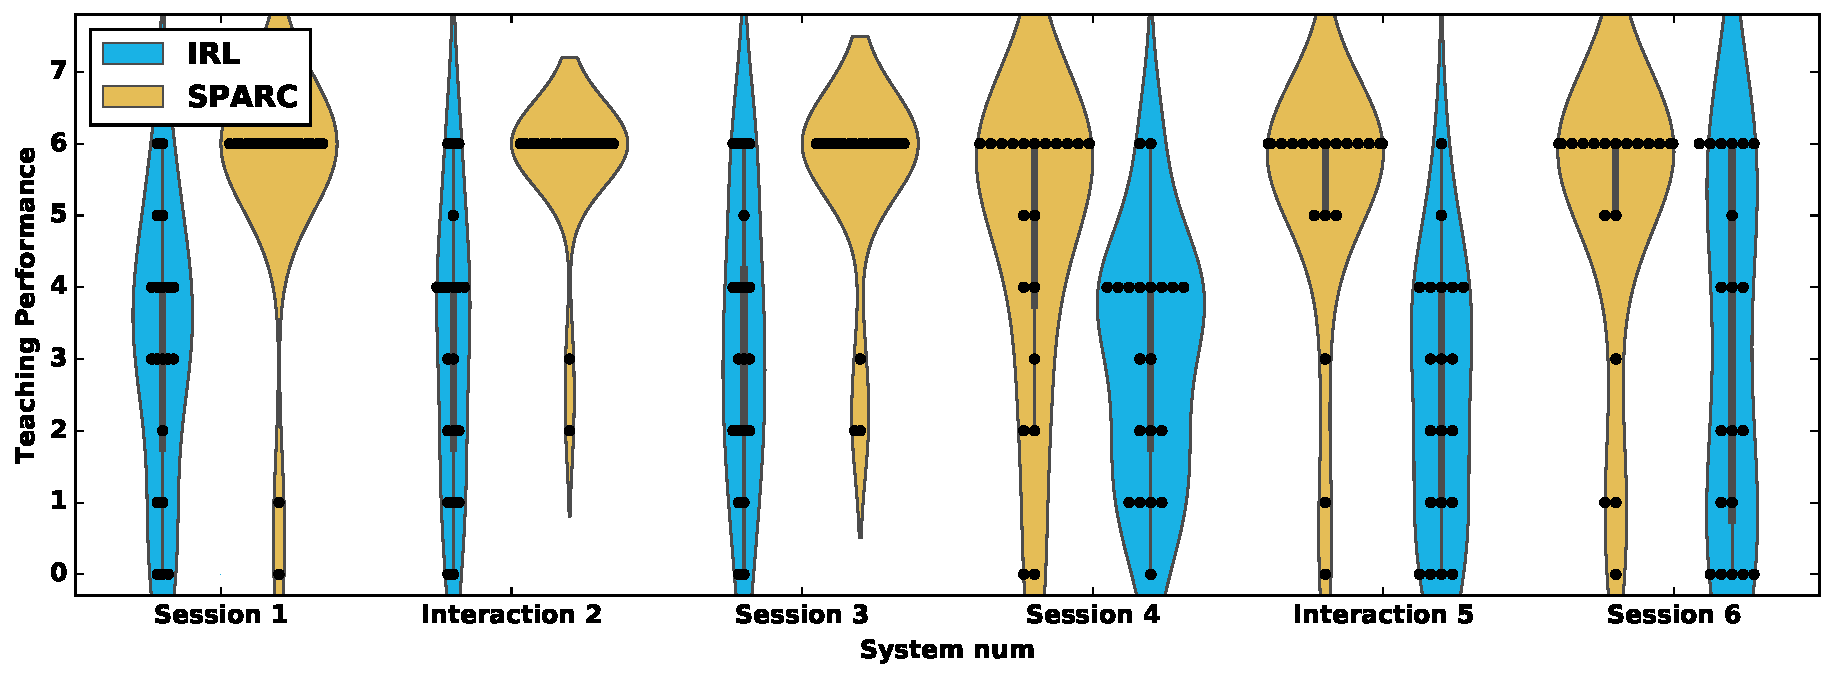
\includegraphics[width=\textwidth]{teaching_performance.pdf}
	\centering
	\caption{Comparison of the teaching performance for the six sessions (the left columns presents the data of participants in group 1 and the right ones those in group 2). The colours are swapped between session 3 and 4 to represent swapping of conditions. A 6 in teaching performance shows that the participant reached at least one success during the teaching phase. The vertical grey lines represent minimal barplots of the data and the shaded areas the probability distribution most likely to produce these results.
	}
	\label{fig:control_teaching_performance}
\end{figure}

\begin{table}[ht]
	\centering
	\caption{Median performance in the teaching phase. Noted that between session 3 and 4 participants change system.}
	\label{tab:control_teaching_perf}
	\begin{tabular}{@{}lllllll@{}}\toprule
		& $\widetilde{X}_{1}$ & $\widetilde{X}_{2}$ & $\widetilde{X}_{3}$ & $\widetilde{X}_{4}$ & $\widetilde{X}_{5}$ & $\widetilde{X}_{6}$\\ 
		\midrule
		IRL & 3.0 & 3.5 & 3.0 & 3.5 & 2.5 & 3.0\\
		SPARC & 6.0 & 6.0 & 6.0 & 6.0 & 6.0 & 6.0\\
		\bottomrule
	\end{tabular}
\end{table}

This higher teaching performance for \gls{sparc} provides partial support for H1 and its prediction: '\gls{sparc} will be more effective and efficient than \gls{irl} when used by non-experts'.

\subsubsection{Testing Performance}

Figure \ref{fig:control_perf} presents the performance of the system during the testing phase, and represents how successful was the participants' teaching. The bayesian mixed ANOVA shows an effect of condition on the performance for both interactions ($B_1=8.8$x$10^5$ and $B_2 = 7340$). The median performance scores in Table \ref{tab:control_perf} show that a higher test performance was achieved when participants used \gls{sparc} compared to when they used \gls{irl}. The session number has no impact on the performance on the first interaction, but results are inconclusive for the impact of repetition on the second interaction ($B_1=0.084$ and $B_2=0.80$).

 %There is a significant difference of performance between systems; a Friedman test shows a significant difference between systems during the first three sessions ($\chi^{2} = 50.8$, $p <.001$) and during the next three sessions ($\chi^{2} = 36$, $p <.001$). Similarly, a significant difference in performance is noted within participants (Order 1: $\chi^{2} = 37.9$, $p <.001$ - Order 2: $\chi^{2} = 55.3$, $p <.001$). 
 %In all the cases, participants interacting with \gls{sparc} achieved a significantly higher performance than those interacting with \gls{irl}, regardless of the order in which they interacted ($p<.05$ for all pairwise comparison). No difference of performance has been observed when using Wilcoxon signed rank test on the three repetitions between participants when interacting with the same system, so interacting for a second or third session with the same system does not have a significant impact on participants' performance.

As shown in Table \ref{tab:control_perf} and Figure \ref{fig:control_perf}, only a limited number of participants succeeded in teaching the robot to complete the task using \gls{irl}, this finding will be discussed in more details in section \ref{sec:control_discussion}.


\begin{figure}[ht]
	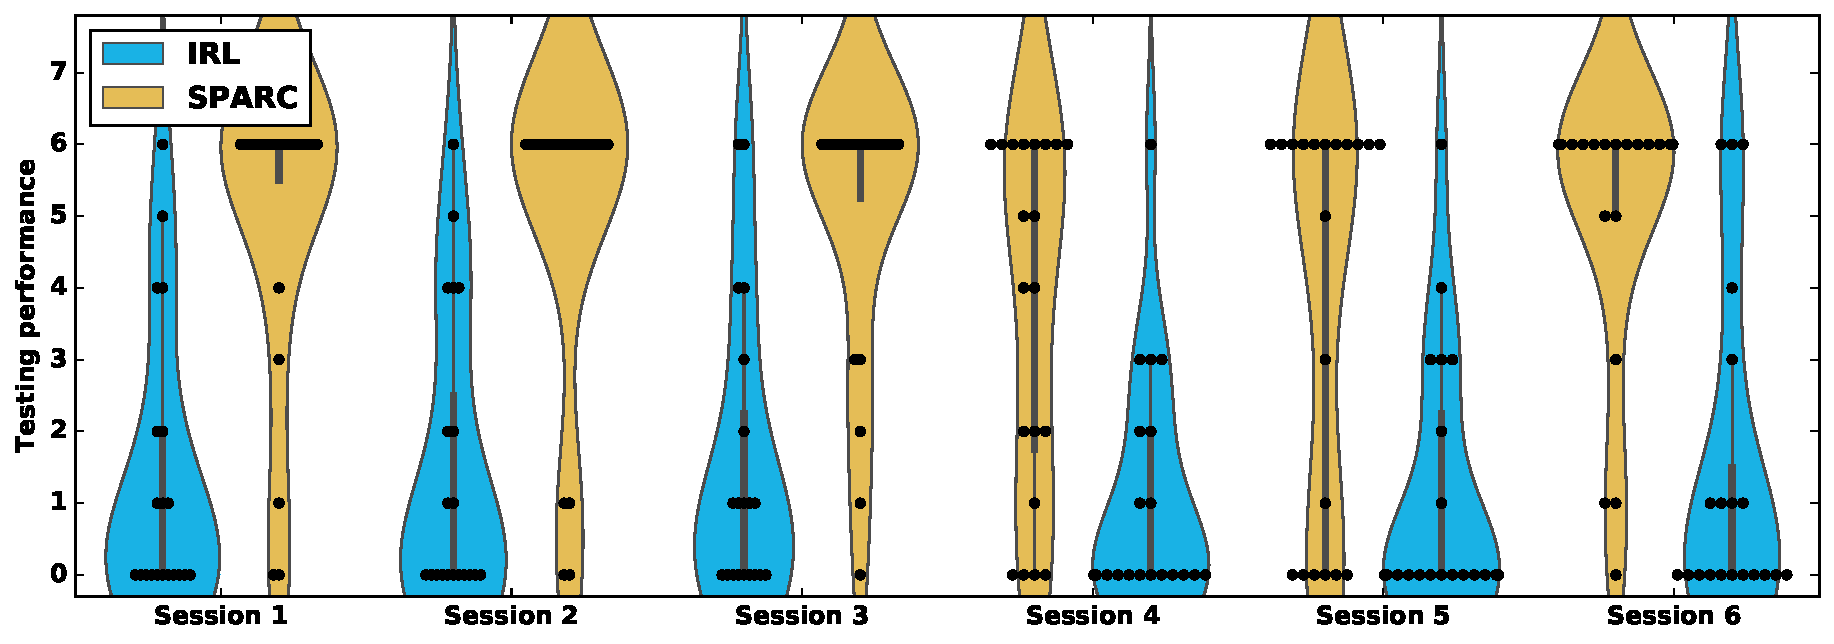
\includegraphics[width=\textwidth]{performance.pdf}
	\centering
	\caption{Comparison of the testing performance for the six sessions. A 6 in performance shows that the taught policy led to a success.
	}
	\label{fig:control_perf}
\end{figure}

\begin{table}[ht]
	\centering
	\caption{Medians of the performance in the testing phase.}
	\label{tab:control_perf}
	\begin{tabular}{@{}lllllll@{}}\toprule
		& $\widetilde{X}_{1}$ & $\widetilde{X}_{2}$ & $\widetilde{X}_{3}$ & $\widetilde{X}_{4}$ & $\widetilde{X}_{5}$ & $\widetilde{X}_{6}$\\ 
		\midrule
    IRL & 0.0 & 0.0 & 1.0 & 0.0 & 0.0 & 0.0\\
    SPARC & 6.0 & 6.0 & 6.0 & 4.5 & 6.0 & 6.0\\
    \bottomrule
	\end{tabular}
\end{table}

This higher testing performance for \gls{sparc} provides partial support for H1 and its prediction.

\subsubsection{Teaching Time}

Figure \ref{fig:control_time} presents the time participants spent teaching. They could stop whenever they decided or the  session would stop automatically after 25 minutes. The bayesian mixed ANOVA shows the important role of condition ($B_1=31.4$ and $B_2 = 679$) and session number on the time spent teaching ($B_1=8.3$x$10^9$ and $B_2 = 3188$). Table \ref{tab:control_time} and additional post-hoc comparisons between the sessions in each interaction indicate that in the first interaction, the teaching time decreases between the first and the second session and then tends to stabilise between the second and the third sessions ($B_{12}=4.4$x$10^5$, $B_{13}=2.6$x$10^6$ and $B_{23}=0.435$). A similar pattern occurs in the second interaction ($B_{45}=850$, $B_{46}=382$ and $B_{56}=0.172$) with more support for a stabilisation of teaching time between session 5 and 6.

\begin{figure}[ht]
	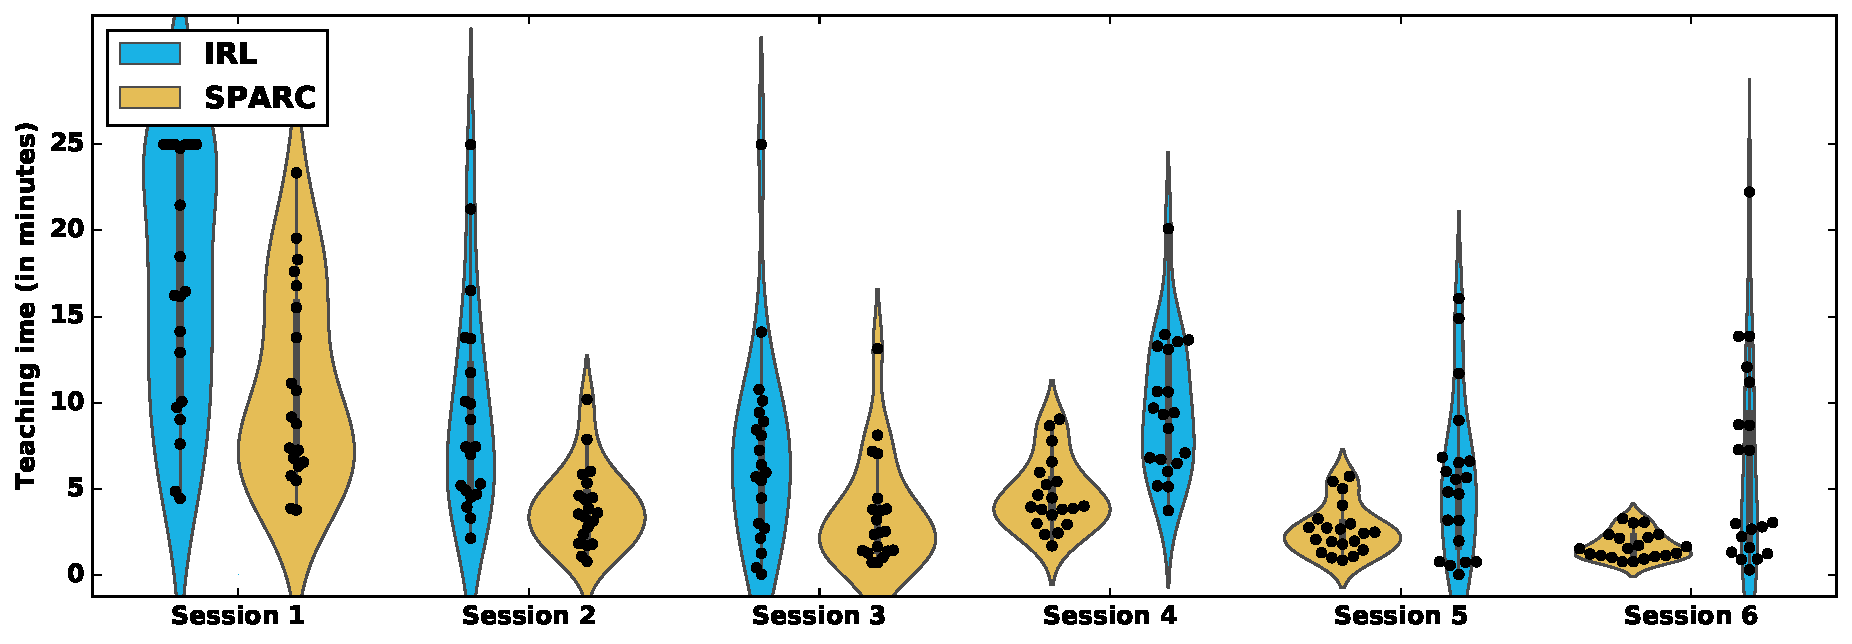
\includegraphics[width=\textwidth]{time.pdf}
	\centering
	\caption{Comparison of the teaching time for the six sessions. At 25 minutes, the session stopped regardless of the participant stage in the teaching.
	}
	\label{fig:control_time}
\end{figure}

\begin{table}[ht]
	\centering
	\caption{Medians of the teaching time in each session (in minutes).}
	\label{tab:control_time}
	\begin{tabular}{@{}lllllll@{}}\toprule
		& $\widetilde{X}_{1}$ & $\widetilde{X}_{2}$ & $\widetilde{X}_{3}$ & $\widetilde{X}_{4}$ & $\widetilde{X}_{5}$ & $\widetilde{X}_{6}$\\ 
		\midrule
    IRL & 16.34 & 7.43 & 6.16 & 9.36 & 5.18 & 3.0\\
    SPARC & 8.97 & 3.56 & 2.49 & 3.96 & 2.45 & 1.53\\
    \bottomrule
	\end{tabular}
\end{table}

Combined with the consistent high performance of \gls{sparc}, this decrease of teaching time indicates that participants managed to learn an efficient way to use \gls{sparc} to teach the robot a successful action policy. On the other hand, this similar decrease of teaching time and the lower performance with \gls{irl} could indicate that participants lost motivation to interact with \gls{irl}. As they did not find an efficient way to teach the robot with \gls{irl}, they dedicate less efforts to try in successive session. These interpretations provide partial support to H1 and its prediction.

\subsubsection{Number of Inputs}
%To write
Figure \ref{fig:control_inputs} presents the number of inputs the participants provided while teaching. The bayesian mixed ANOVA shows that in both interactions, the condition had an impact on the number of inputs provided ($B_1=27.4$ and $B_2 = 34.1$). On the other hand,  the session number only had a clear impact for the first interaction, the results are inconclusive for the second interaction ($B_1=4.1$x$10^5$ and $B_2 = 1.5$). Table \ref{tab:control_inputs} and additional post-hoc comparisons between sessions indicate that in the first interaction, the number of inputs used decreases between the first and second sessions and then tends to stabilise between the second and the third sessions($B_{12}=2707$, $B_{13}=4.7$x$10^4$ and $B_{23}=0.410$). Similarly, for the second interaction, a difference tends to be observed between session 4 and 5 and session 4 and 6 while the number of inputs is similar between session 5 and 6 ($B_{45}=2.6$, $B_{46}=2.7$ and $B_{56}=0.17$).

\begin{figure}[ht]
	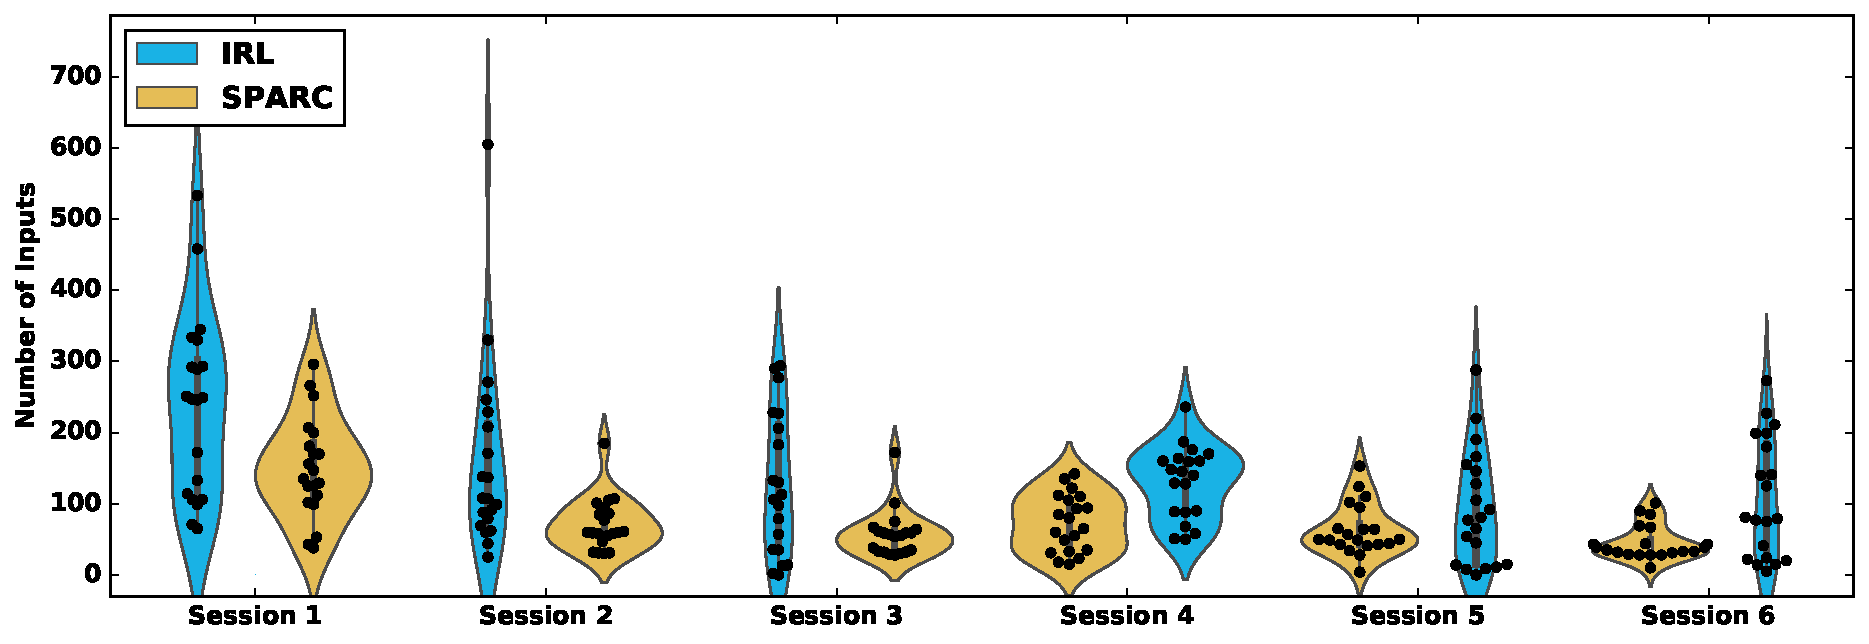
\includegraphics[width=\textwidth]{inputs.pdf}
	\centering
	\caption{Comparison of the number of inputs provided by the participants for the six sessions. 
	}
	\label{fig:control_inputs}
\end{figure}

\begin{table}[ht]
	\centering
	\caption{Medians of the number of inputs in the testing phase.}
	\label{tab:control_inputs}
	\begin{tabular}{@{}lllllll@{}} \toprule
		& $\widetilde{X}_{1}$ & $\widetilde{X}_{2}$ & $\widetilde{X}_{3}$ & $\widetilde{X}_{4}$ & $\widetilde{X}_{5}$ & $\widetilde{X}_{6}$\\ 
		\midrule
    IRL & 248.0 & 107.5 & 109.5 & 142.5 & 79.0 & 80.0\\
    SPARC & 141.0 & 60.0 & 56.0 & 72.5 & 50.0 & 37.0\\
    \bottomrule
	\end{tabular}
\end{table}

Similarly to the teaching time, this reduction of inputs provided during the teaching, while maintaining a high performance for \gls{sparc} offers partial support for H1 and its prediction.

\subsubsection{Number of Failures}

Figure \ref{fig:control_failures} presents the number of failure states participants encountered during the teaching phase. The bayesian mixed ANOVA shows that for both interactions, both the condition ($B_1=6.2$x$10^4$ and $B_2 = 2.6$x$10^4$) and session number ($B_1=1.5$x$10^4$ and $B_2 = 11$) play an important role on the number of failures. Table \ref{tab:control_failures} and additional post-hoc comparisons between sessions indicate that in the first interaction, the number of failures decreases between the first and the second session and then stabilises between the second and the third one ($B_{12}=619$, $B_{13}=1.7$x$10^3$ and $B_{23}=0.25$). Similar results can be observed in the second interaction ($B_{45}=3.3$, $B_{46}=7.5$ and $B_{56}=0.2$).

\begin{figure}[ht]
	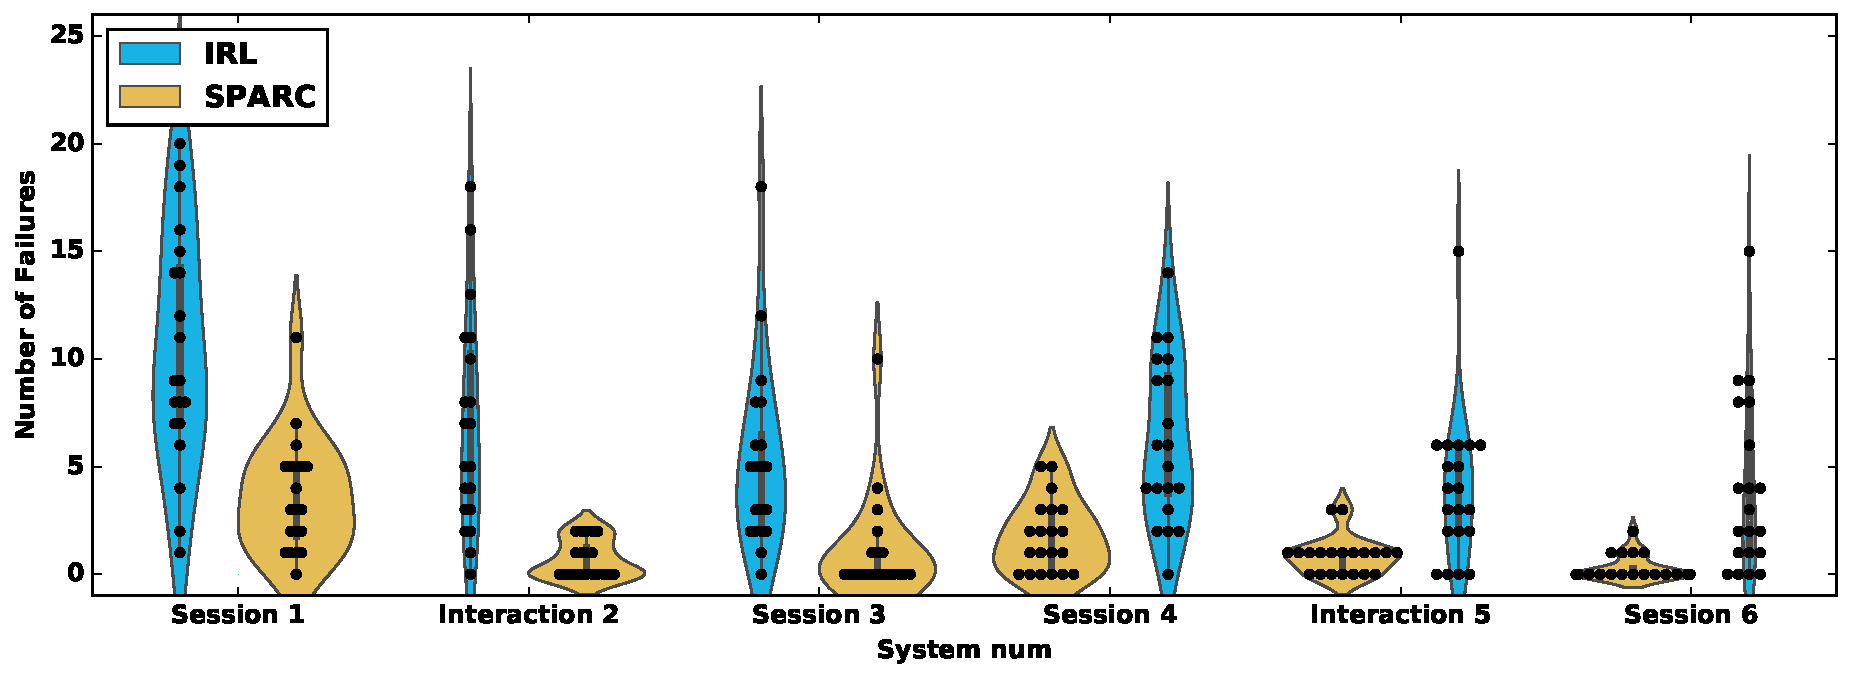
\includegraphics[width=\textwidth]{failures.pdf}
	\centering
	\caption{Comparison of the number of failures for the six sessions.
	}
	\label{fig:control_failures}
\end{figure}

\begin{table}[ht]
	\centering
	\caption{Medians of the number of failures in the testing phase.}
	\label{tab:control_failures}
	\begin{tabular}{@{}lllllll@{}}\toprule
		& $\widetilde{X}_{1}$ & $\widetilde{X}_{2}$ & $\widetilde{X}_{3}$ & $\widetilde{X}_{4}$ & $\widetilde{X}_{5}$ & $\widetilde{X}_{6}$\\ 
		\midrule
	    IRL & 9.0 & 6.0 & 5.0 & 5.5 & 3.5 & 2.5\\
	    SPARC & 3.0 & 0.0 & 0.0 & 1.5 & 1.0 & 0.0\\
	    \bottomrule
	\end{tabular}
\end{table}

The fewer failures faced when using \gls{sparc} compared to \gls{irl} offers partial support to H1 and its prediction. Additionally, the low number of failures when using \gls{sparc} in the last sessions of both interaction (sessions 3 and 6) shows that participants became more efficient with \gls{sparc}, reaching successes without facing failures, which partially support H2: `SPARC can be used by expert users (knowledgeable in the interaction process) to teach an action policy safely, quickly and efficiently'.

\subsection{Questionnaire Data}

The main task of the post-interaction questionnaires was to assess the workload on participants when interacting with a condition using the NASA-TLX questionnaire. Figure \ref{fig:control_workload} presents the workload for participants for each condition for both interactions (the average of the six ratings from 0 to 20 for each category). In the first interaction, participants using \gls{irl} reported an average workload of 12.9 ($SD=2.33$), whereas the ones using \gls{sparc} reported 8.94 ($SD=3.01$). In the second interaction, participants interacting with \gls{irl} had an average workload of 13.87 ($SD=2.84$) and the ones using \gls{sparc} reported 7.44 ($SD=3.41$). Bayesian independent t-test show a strong effect on the condition for both interactions ($B_1=462$ and $B_2=8.1$x$10^4$) between participants. And bayesian paired t-test show a similar effect of the condition within participants for both orders (order 1: $B_{IRL-SPARC}=1.7$x$10^6$ - order 2: $B_{SPARC-IRL}=1.1$x$10^4$). Regardless of the comparison criteria (between or within subjects), participants reported a lower workload when interacting with \gls{sparc} than when interacting with \gls{irl}.

\begin{figure}[ht]
	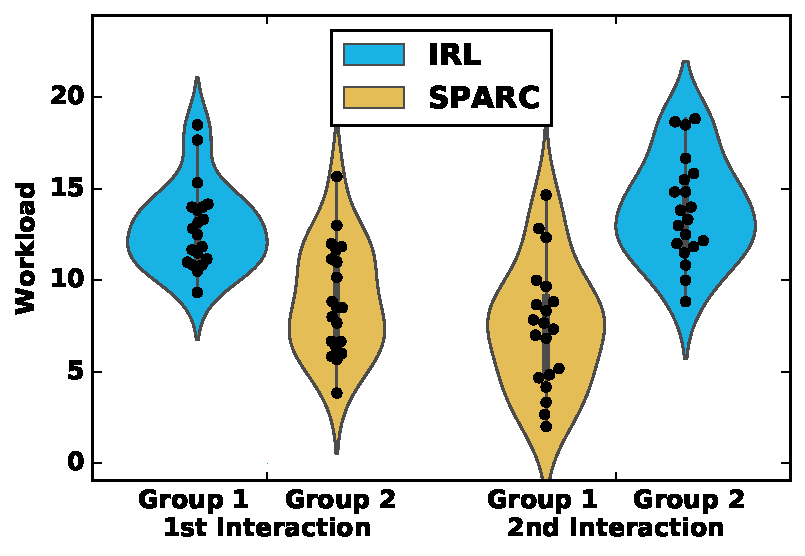
\includegraphics[width=.5\textwidth]{workload.pdf}
	\centering
	\caption{Average workload for each participants as measured by the NASA-TLX for each conditions in both interaction order.
	}
	\label{fig:control_workload}
\end{figure}

This lower workload when using \gls{sparc} compared to \gls{irl} offers partial support for H1 and its predictions.

\subsection{Expert} \label{ssec:control_expert}

To evaluate the best case potential offered by \gls{sparc} and \gls{irl}, an expert in \gls{hri} knowing the detail of the algorithm and the interactions (the author) interacted five times with each system. For both systems, the expert followed a strictly optimal strategy. In the case of \gls{irl} the optimal strategy consisted on providing as much guidance as possible, rewarding positively correct actions and negatively incorrect ones. For \gls{sparc} the optimal strategy consisted on providing commands for every single action to demonstrate an optimal trajectory to the robot. This shows the expected behaviours in optimal conditions, the best metrics achievable. Results of the interactions are presented in Table \ref{tab:control_expert}. In both cases, the expert successfully taught the robot (as indicated by a performance of 6 during the teaching and the test), which indicates that both systems can be used to teach a robot an action policy. However as demonstrated by a bayesian independent t=test, the time required to teach the robot with \gls{irl} is higher than with \gls{sparc} ($B=7102$). 

\begin{table}[ht]
	\centering
	\caption{Results of an expert interacting 5 times with each system following an optimal strategy. When the variance is 0, Bayes Factor cannot be computed.}
	\label{tab:control_expert}
	\begin{tabular}{@{}llll@{}}\toprule
		&IRL \textit{M(SD)} & SPARC \textit{M(SD)} & $B$ factor\\
		\midrule
		Performance & 6 (0) & 6 (0) & NA \\
		Time (minutes) & 4.5 (0.67) & 0.60 (0.03) & 7102 \\
		Inputs & 115.6 (8.4) & 28 (0) & NA \\
		Number of Failures & 3.2 (0.84) & 0 (0) & NA \\
		\bottomrule
	\end{tabular}
\end{table}

Additionally, when using \gls{irl}, even an expert cannot prevent the robot from reaching failure states during the teaching due to the lack of control over the robot's action. Conversely, when interacting with \gls{sparc}, due to the full control and clear communication, the teacher can ensure that only desired actions are executed. So with sufficient knowledge of the interaction possibilities, an expert can teach the robot to behave safely without having to explore and reach undesired states using \gls{sparc}. This has real world applications in \gls{hri}, as random exploration is often impossible or undesirable when interacting with humans. \gls{sparc} offers a way for the teacher to stop the robot from executing actions with negative consequences whilst still guiding the robot toward useful parts of the environment.

Similar results to these were observed with our non-expert participants: in their last session with \gls{sparc}, both groups had a median of 0 failures and a performance of 6. This indicates that more than half of the participants successfully taught the robot the task without ever hitting a failure state after gaining understanding of \gls{sparc} in their first and second interaction with it.

The absence of failures, the lower number of inputs and the shorter time required to teach with \gls{sparc} compared to \gls{irl} when used by an expert user provide support for H2.
%\section{Discussion}

\section{Validation of the Hypotheses}

\subsection{Effectiveness and Efficiency with Non-Experts}
The objective metrics show that despite spending a shorter time interacting with \gls{sparc} and using fewer inputs, participants reached a higher performance than with \gls{irl} and faced fewer failures during teaching. Additionally, when interacting with \gls{sparc}, the time participants took to teach the robot decreased to reach a plateau in the second and third sessions, without negatively affecting the performance. This indicates that after the first session, participants understood the interaction mechanism of \gls{sparc} and consistently managed to achieve a high performance whilst requiring less time to teach the robot the task. On the other hand, when interacting with \gls{irl}, participants' performance remained low over the sessions, and their teaching time decreases between session 1 and 2 but not further between session 2 and 3. This decrease of teaching combined with low performance might be due to a loss of motivation after session 1 where often participants did not succeed to teach the robot, reducing the desire to further interact in successive sessions. The results suggest that teaching the robot using \gls{sparc} allows the robot to achieve a higher performance than with \gls{irl}, in a shorter time, while requiring fewer inputs and making fewer errors when teaching. This conclusion is supported by subjective measures: the workload on the teacher is lower when using \gls{sparc} than when using \gls{irl}. 

For these reasons, H1 and its prediction is ( `Compared to \gls{irl}, \gls{sparc} can lead to higher performance, whilst being faster, requiring fewer inputs and less mental effort from the teacher and minimising the number of errors during the teaching when used by non-experts.') is supported.

\subsection{Safety with Experts}

As presented in Section \ref{ssec:control_expert}, when interacting with \gls{sparc}, an expert can reach a success easily and safely (requiring a low number of inputs and a short time and without facing a single failure). This effect is also observed after some training for the naive participants: most of them reached a success without encountering any failures in their last session with \gls{sparc}.

However, when interacting with \gls{irl}, even the expert applying a strictly optimal policy cannot prevent the robot reaching failures states. This effect is due to the lack of control of feedback-based \gls{iml} methods. As teachers only rate the actions of the agent, they cannot prevent the learners from making errors. They can only negatively reward these errors to reduce their chance of being selected in the future. While the guidance allows to partially mitigate this effect, the presence of actions not covered by this guidance limits the its efficiency during the teaching.

This difference shows support for H2 (`\gls{sparc} can be used by expert users to teach an action policy safely, quickly and efficiently, achieving better results other \gls{iml} methods lacking control'). This also demonstrates how the principles presented in Chapter \ref{chap:sparc} provide control to the teacher over the robot's actions and by extend improve the teaching. Consequently, the principles underlying \gls{sparc} ensure that even in the early stages of teaching (when the robot's action policy is not mature to correctly select actions without supervision), the action policy of the robot is appropriate, which is not the case of most other \gls{iml} methods (as demonstrated by the number of failures when teaching with \gls{irl}).

\subsection{Control}
\label{ssec:control_control}

One of the main differences between the two methods is the way in which the concept of teaching is approached. With \gls{irl} an exploratory individual learning approach is followed: the robot has the freedom to explore, whilst receiving feedback on its actions and limited guidance about what action to pursue next from a teacher. This social aspect of the teaching: with hints and guidance, partial control over the robot actions and bidirectional communication is inspired by the way humans teach. While not every member of the population is knowledgeable about \gls{ml}, they are experienced with social learning \citep{thomaz2008teachable}. This similarity between how humans teach robots and other humans has also been supported by behaviours displayed by participants in the original study. Participants gave motivational rewards to the robot, just as one would do to keep a child motivated during learning, despite the absence of effect or use in classical reinforcement learning \citep{thomaz2008teachable}.

On the other hand, \gls{sparc} promotes a more direct teaching process: the supervisor explicitly tells the robot what to do and expects it to obey and learn. The robot is not totally considered as a social agent from the supervisor's point of view, but rather as a tool having to learn an action policy. This does not mean that the robot cannot be social: the supervisor can teach the robot in a non-social way how to interact socially in a non-social way. This approach is more task oriented, and we argue that it better fits many applications of \gls{hri} when the interaction with the teacher does not have to be social. For example, in \gls{sar}, the task (such as interaction with a child with \gls{asd}) is more important than the social relationship between the robot and its supervisor (a therapist for example) and as such the relevance of the social side of the interaction between the teacher and the robot is reduced.

The post-experiment questionnaire included the open question: `which robot did you prefer interacting with and why?'. Almost all the participants (38 out of 40) replied that they preferred interacting with \gls{sparc}. Half of all the participants used vocabulary related to the control over the robot's actions (`control', `instruction', `command', `what to do' or `what I want') to justify their preferences without these words being used in the question. Furthermore, multiple participants reported being frustrated not to have total control over the robot's actions with \gls{irl}, they would have preferred being able to control each of the robot's actions. 

To the question `which interaction was more natural?', 10 participants rated \gls{irl} as being more natural, using justifications such as: `The robot thinks for itself', `Some confusion in the [\gls{irl}] robot was obvious making it more natural', `More like real learning', `Because it was hard to control the robot' or `People learn from their mistakes faster'. But despite these participants acknowledging that \gls{irl} is more `natural', closer to human teaching, they still preferred teaching using \gls{sparc}. This suggests that when humans teach robots, they are focused on the outcome of the teaching, on the learner's proficiency in the task. As mentioned previously, this might relate to the role of robots, they often interact in human-centred scenarios where they have to complete a task for their users. And, due to the absence of life-long learning for robots today, it is not worth investing time and energy to allow the robot to improve its learning process or explore on its own. These comments from the participants show support for H3 (`Teachers prefer a method providing more control over the robot's actions.').

\section{Discussion}
\label{sec:control_discussion}

Despite not being originally designed for use in combination with \acrlong{rl}, \gls{sparc} achieved good results in this study. This shows that principles presented in Chapter \ref{chap:sparc} are agnostic to the learning algorithm and promote an efficient teaching interaction. Furthermore, \gls{sparc} achieves a higher performance, in a shorter time and facing less failures than \gls{irl}, whilst requiring a lower workload from the human teacher. And finally, when used by experts (designer or trained participants), \gls{sparc} demonstrates that teaching can be safe and quick: the full control over robot's action in the teacher's hands ensures that only desired actions will be executed. These results show an important feature of teaching robots to interact in human environments. As robots interact in task oriented, human-centred environments, human teachers need approaches with direct control and more focused on commands rather than letting the robot explore on its own and only evaluate its actions.

\subsection{Comparison with Original Interactive Reinforcement Learning Study}

%Mention that regardless of the learning algorithm, participants had issues to guide the robot to the right parts of the environement due to the limited guidance

Unlike the original experiments evaluating \gls{irl} \citep{thomaz2008teachable}, in this study, most of the participants did not succeed in teaching the robot the full cake baking sequence using feedback and guidance (the \gls{irl} condition). In Thomaz and Breazeal's study, the participants were knowledgeable in machine learning: when asked to rate their expertise in \gls{ml} software and system (1=none, 7=very experienced), they reported an above average score (M=3.7, SD=2.3), but the population in the presented study was drawn from a more general public having little to no knowledge of machine learning (M=1.8, SD=1.13 - on a 5-item Likert scale). This can explain why a much larger number of participants did not achieve success with \gls{irl} in this study whereas Thomaz and Breazeal only reported 1 participant out of 13 failing the task. In our study, only 12.5\% of the participants and the expert did manage to teach the robot using \gls{irl}. 

As demonstrated by the teaching performance, most of the participants did not manage to reach a single success even during the teaching phase in the \gls{irl} condition. We identify the lack of control over the robot's actions as a limiting factor for the teaching, as participants did not manage to steer the robot to do correct actions, they could not reward them and teach the robot an efficient action policy. Additionally, the requirement of explicit feedback made the learning task more complex. Participants often did not reward an action after a guidance, assuming that informing the robot what it should do did not require an additional explicit reward. Teachers of robots need to have control over the robot's action and robots should also use implicit rewarding to ease the task for the teacher. For example, \gls{sparc} uses implicit rewarding by automatically providing a positive reward to actions selected by the teacher and also every action not corrected by the teacher as it has been implicitly validated. This is consistent with \cite{kaochar2011towards} who note that feedback is not well suited for teaching an action policy from scratch, but better for fine tuning. For teaching the basis of the action policy, they recommend using demonstrations, a method much closer to \gls{sparc}. 

\subsection{Advantages and Limitations of SPARC}

In the implementation of \gls{sparc} for this study, the algorithm mostly reproduces actions selected by the teacher. One could argue that no learning algorithm is required, instead the actions could just be blindly reproduced by the robot. However, when combined with reinforcement learning, \gls{sparc} does provide advantages. As a state visited multiple times in an episode is considered as a single identical state for the learning algorithm, loops in the demonstrations can be removed for future executions of the action policy. Additionally, this provide the algorithm with a way to deal with variations in teaching. It allows the robot to reach a success from the initial state but also to continue the action policy from any state in the trajectory. And finally, due to the suggestion/correction mechanism, the teacher can let the robot act on its own only intervening when the robot is about to execute an incorrect action. 

%PRobably not required
%Over the 79 successful trials using \gls{sparc}, participants used 47 different strategies to teach the robot the task of baking a cake. This shows how \gls{sparc}, as a single control mechanism, allows for different action policies to be learnt depending on the person teaching the robot. With \gls{sparc} the robot can adapt its behaviour to the human it is interacting with, profiling the user to find the desired way of behaving.

However \gls{sparc} also has limitations in the current implementation, related to the quality of the human supervised guidance. If the teacher allows an action to be executed by mistake (through inattention or by not responding in time), this action will be reinforced and will have to be corrected later on. This might lead to loops when successive actions are returning to a previous state (such as move left, then right). In that case, the teacher has to step in and manually guide the robot to break this cycle. Furthermore, due to the automatic execution of actions, the teacher has to be attentive at all times and ready to step in when a wrong action is suggested by the robot. This is a limitation as a lack of supervision can lead to undesired reinforcement of incorrect behaviours.

In this study, \gls{sparc} has been applied to a scenario where a clear strategy with optimal actions was present. The interaction also took place in a virtual environment with a discrete time and a limited number of states. Real human-robot interactions are stochastic, happen in real time and often there is no clear strategy known in advance, and as such present limited similarity with this study. However, in these real \gls{hri}, human experts in the application domain know what type of actions should be executed when, and which features of the environment they used for their decision. And, as this knowledge might not be available to the robot's designers or could be complex to formalise in a set of rules a robot should follow, robots should be able to learn from a domain user in an interactive fashion. And this study presented a simple environment allowing us learn more about how humans could teach a robot using \gls{sparc}.

The limitations of this study (simulated deterministic world, limited number of state, discretisation of time and absence of interaction with humans) have been addressed in Chapter \ref{chap:tutoring}. In the study presented in that chapter, \gls{sparc} has been applied to a real-world social interaction with humans, possessing all the challenges typical to these interactions: complex non-deterministic world, with continuous time, real impact of actions and importance of the social factors in the interaction.

%PRobably not required
%Nevertheless, we argue that \gls{sparc} allows for easy and safe teaching due to the presence and control by the teacher. And the suggestion/correction mechanism with automatic execution of actions allows for a smooth teaching process where the workload on the teacher can decrease over time as shown in \cite{senft2015sparc}. The workload of the teacher when starting is relatively high, when the robot has no information on which actions to take yet, and decreases over time requiring only limited intervention by the teacher.

%MIght be put in the final discussion
\subsection{Lessons Learned on Designing Interactive Machine Learning for HRI}

From observing participants interacting with both systems, we derived four recommendations for future designs of interactive learning robot that we also used to develop the study presented in Chapter \ref{chap:tutoring}. 

\subsubsection{Clarity of the Interface and Transparency}

Algorithms used in machine learning often need precisely specified inputs and outputs and require an internal representation of the world and policies. These variables are often not accessible to a non expert: the weights of a neural network or the values in a Q-table are not easily interpretable, if at all. The inner workings of the machine learning algorithms are opaque, and people only have access to inputs and outputs of the black box that is machine learning. As such, care needs to go into making the input and output intuitive and readable. For example, in this study (following Thomaz and Breazeal's original study), the communication between the robot and the teacher occurred through the environment: using clicks on objects rather than a more classical \gls{gui} with buttons. This design decision had important consequences: as the interface is not explicit, participants first had to familiarise themselves with the interface, discover how to interpret the robot's behaviour, which actions are available for each state and learn the exact impact of the robot's actions. This lack of clarity led to a high number of failures and high teaching time during the first session in our study. So, we argue that to avoid this precarious discovery phase for the teachers, roboticists have to design interfaces taking into account results from the Human Factors community as advocated by \cite{adams2002critical}, such as including the users in the design process or finding intuitive ways to train teachers to use these interfaces.

\subsubsection{Limits of Human Adaptability}

Human-Robot Interaction today is facilitated by relying on people adapting to the interaction, often making use of anthropomorphisation \citep{zlotowski2015anthropomorphism}. Roboticists use people's imagination and creativity to fill the gaps in the robot's behaviour. However, human adaptivity has its own limits: in our study, often participants adopted one particular way of interacting with the system and they held on to it for a large part of the interaction. For example, participants clicked on an object requiring two actions to interact with, assuming that the robot had planning capabilities which it did not. Or when the robot was blocked in some cycles (due to constant negative reward in and undo behaviour \gls{irl} or a loop created and not stopped with \gls{sparc}), participants kept on trying the same action to break the loop, without really exploring alternatives. For these reasons, if robots are to be used by a naive operator, they need mechanisms to detect these `incorrect' uses, and either adapt to these suboptimal human inputs or at least inform the user that this type of input is not efficient and clarify what human behaviour is appropriate instead.

\subsubsection{Importance of Keeping the Human in the Learning Loop}

As argued in previous chapters, we think the presence of a human in the learning process is key. This human has the opportunity to provide important knowledge about the environment and allow the machine learning to deal with sensor errors or imperfect action policies. As in real world a robot's behaviour can hardly be perfect, keeping a human in the learning loop allows to continue improving the robot's behaviour even after an acceptable policy is reached. This is different to most of the \gls{lfd} approaches where the robot is left unsupervised to interact once an action policy is learned \citep{argall2009survey,sequeira2016discovering}. This was one of the important points we considered when proposing \gls{sparc}: there is no distinction between a teaching and a testing phase, they are merged into a single phase, moving away smoothly from \gls{woz} to \gls{sa}. The teacher can correct the robot when needed and let it act when it behaves correctly. In this study, participants used this feature of \gls{sparc}: many participants corrected \gls{sparc} only when required rather than forcing every action. For example, 37.5\% of the participants even let the robot complete the task once without giving a single command before starting the test to be sure that the robot was ready. This demonstrate that keeping the human in the learning loop is important to ensure that the robot's behaviour stays appropriate; and this study demonstrated that \gls{sparc} allows human teachers to be actively involved in the teaching process without requiring important workload for them.

\subsubsection{Keeping Teachers in Control}

Most of the scenarios where a robot has to learn how to interact with humans are human-centred: the robot has to complete a task to help a human (such as \gls{sar}). In these scenarios, the goal of learning is to ensure that the robot can complete the task it has been assigned, not to provide the robot with tools to learn more efficiently in further interactions. Accordingly, participants in our study did not desire to have the robot exploring on its own and learn from its experience, they wanted to be able to direct the robot (see Section \ref{ssec:control_control}). In addition to reducing the effectiveness of the learning, a lack of control over the robot's actions can lead to frustration and loss of motivation for the teacher as shown with the results of \gls{irl} in this study. This human control is especially critical when the robot is designed to interact with other people because undesired actions can have a dramatic impact, such as causing physical or mental harm for the interaction partners or bystanders. For these reasons, we argue that when designing an interactively learning robot for \gls{hri} in human-centred scenarios, it is critical to keep the human teacher in control. 

However, this control does not mean that the robot cannot learn and become autonomous. We take a stronger inspiration from \gls{lfd}, using human input more efficiently to guide the learning, speeding it up and making it safer, especially in the early stages of the learning. With \gls{sparc} the human is in control during all  the interaction, but especially when the robot is prone to making exploratory mistakes, so that the teacher can prevent them before they occur. But once the action policy is appropriate enough, the teacher can leave the robot to interact mostly on its own, providing only limited supervision to refine the action policy.

%\subsection{Future work}
%\label{ssec:future}
%We are currently working on a new experiment in which people interacting with a robot in a continuous time and non-deterministic environment. In this experiment, the teacher is able to send commands to the robot, provide rewards and identify features in the environment they consider important. The learning algorithm will take these inputs into account and combine them with interaction metrics to learn. An approach could be to use the actor-critic paradigm: the critic being an objective evaluation of the action results (environmental rewards), and the actor using results from the critic and teacher's guidance to update the action policy.

\section{Summary}

As presented in Chapter \ref{chap:sparc}, \gls{sparc} has been designed to allow naive humans to teach an action policy to a robot while maintaining an appropriate behaviour. This chapter presented a study where \gls{sparc} was combined with \gls{rl} to teach a simulated robot to complete a baking task. \gls{sparc} used intentions communicated by the robot, full control over the robot's behaviour and an implicit rewarding mechanism to allows participants teach the robot an action policy. A study involving 40 participants compared this approach with \gls{irl}, another \gls{iml} approach using communication of uncertainty, partial control and explicit rewarding to teach the robot. When interacting with \gls{sparc}, participants took less time and fewer inputs to reach more successes, whilst facing fewer failures. Participants also reported a lighter workload when using \gls{sparc} than when interacting with \gls{irl}. This study, demonstrated that \gls{sparc} is usable by naive participants to successfully teach a robot an action policy quickly and safely.

Based on these results and our observations of the participants, we propose four guidelines to designing interactive learning robots: (1) the interface to control the robot should be intuitive, (2) the limits of human adaptability have to be taken into account (robots should detect deadlocks in human behaviours and adapt how they are controlled or inform the human about these incorrect behaviours), (3) the operator should be kept in the learning loop and (4) teachers should stay in control of the robot's behaviour when interacting in a sensitive environment (such as \gls{rat}). The first two points can be seen to apply to all robot teaching methods, and should be addressed at the time of designing the interface. And, by definition, \gls{sparc} aims to address these last two points: maintaining the performance of an adaptive system by remaining under progressively decreasing supervision.

In summary, this chapter extended \gls{sparc} and compared it to other methods from the \gls{iml} field. \gls{sparc} succeeded in its goal, allowing participants to teach easily and safely an action policy to a robot. Finally, insights from this study have been used to guide the design of study presented in Chapter \ref{chap:tutoring}, the final study of this research, which involves teaching a robot to interact with humans in real-world \gls{hri}.



\cleartooddpage

\chapter[Study 3: Application of SPARC to Tutoring]{Study 3: \\Application of SPARC to Tutoring}\label{chap:tutoring}
\glsresetall
\graphicspath{{images/tutoring/}}

\begin{framed}
	\textbf{Key points:}
	
	\begin{itemize}
		\item Design of an experiment to test \acrshort{sparc} in an educative application with children.
		\item Design and use of a new learning algorithm adapted from nearest neighbours to teach quickly and efficiently in an online fashion.
		\item Between participants study involving 75 children comparing 3 conditions: a passive robot, a supervised robot and an autonomous robot.
		\item Psychology PhD student teaching the supervised robot using \acrshort{sparc}.
%		\item No significant differences of child learning between conditions.
		\item Similar children behaviours with the autonomous and supervised robot, and different to the passive robot.
		\item Demonstration of the applicability of \acrshort{sparc} to teach a robot online an action policy to interact with humans.
	\end{itemize}
\end{framed}

Parts of the work presented in this chapter have been published verbatim in \cite{senft2017toward} and \cite{senft2018robots}, additional publication are under review \footnote{Note about technical contribution in this chapter: the author extended code the freeplay sandbox, see \url{https://github.com/freeplay-sandbox/} and forks.}. The final publications are available from AAAI, EPFL via:
\begin{itemize}
	\item \url{https://aaai.org/ocs/index.php/FSS/FSS17/paper/view/16011}.
	\item \url{https://r4l.epfl.ch/files/content/sites/r4l/files/HRI2018/proceedings_2018/paper4.pdf}.
\end{itemize} 

\newpage

\section{Motivation}

Chapters~\ref{chap:woz} and~\ref{chap:control} tested the \gls{sparc} in interactions between robots or in a virtual world but not for \gls{hri} as it was intended to be used. As such, this Chapter addresses the thesis of this research and evaluates if \gls{sparc} can efficiently be used to teach a robot an interactive behaviour for real human-robot interactions. \gls{hri} in the wild typically occur in constrained but underspecified environments where social behaviours play an important role.  This study takes place in the context of robot tutors for children in education. Tutoring is a framework widely used in \gls{hri} and providing opportunities for a rich and complex interaction between a child and a robot~\citep{leyzberg2012physical,kennedy2015robot}. This scenario and the code are based on \cite{lemaignan2017free} but have been adapted to provide a new teaching task (teaching game and protocol), a knowledge test, a specific robot controller, a learning algorithm and an interface with the teacher supporting \gls{sparc}.

%This study aims to explore if \gls{sparc} can be used to teach a robot an efficient action policy. As such, three conditions have been compared: a passive robot (not providing any support), a supervised robot (learning from a human teacher and supporting the child) and an autonomous robot (applying the learned behaviour). These three conditions, with the passive robot as a control condition, allow us to study both the teaching process and the efficiency of the taught behaviour when being executed without supervision.

\section{Scope of the Study} \label{sec:tutoring_scope}

The main goal of this study was to explore the thesis proposed in this work: ``A robot can learn to interact meaningfully with humans in an efficient and safe way by receiving supervision from a human teacher in control of the robot's behaviour''. This thesis can be divided into two parts: ``a robot can learn safely by receiving supervision from a human teacher'' and ``after learning, such a robot would have a meaningful interaction with humans''. To address these two statements, a study comparing three conditions was designed. In the control condition, the `passive' condition, the robot is not interacting with the child during the learning task. This condition provides a benchmark against which the other conditions can be compared to evaluate the `meaningfulness' and efficiency of the robot's behaviour. In the second condition, the `supervised' condition, the robot is being supervised and taught by a human teacher using \gls{sparc}. This condition is the one in which the robot learns, and can be used to evaluate the impacts of the principles underlying \gls{sparc} when teaching a robot to interact with humans. Lastly, in the `autonomous' condition, the robot applies the learnt policy to interact without supervision with the children. This condition aims at exploring how different the autonomous policy is from the supervised one, and evaluating if the teaching from the human was successful.

These conditions allow us to explore the statements presented above through three hypotheses:
\begin{itemize}
	\item [H1] The autonomous robot is able to interact socially and efficiently during the game sessions and maintain the child's engagement during the learning task.
	\item [H2] An active robot (supervised or autonomous) supports child learning: learning gain in passive condition $<$ learning gain in autonomous condition $<$ learning gain in supervised condition.
	\item [H3] Using \gls{sparc}, the workload on the supervisor decreases over time: the number of corrected actions and the number of actions selected  by the teacher decrease with the progress in the sessions, while the number of correct actions increases.
\end{itemize}

\section{Methodology}

\subsection{Participants}

Children from five classrooms from two different schoold in Plymouth were recruited to take part in the interaction. As both schools have an identical OFSTED evaluation (both school ``require improvement''), all the children were combined into a single pool of participants. Full permission to take part in the study and be recorded on video was acquired for all the participants. In total, 119 children participated in the study, however not all of them have been included in the final analysis. Some participants took part in two pilot versions, with previous versions of the game or the protocol. For other participants, a breach in the protocol have prevented them to be included (such as freezing of the tablet due to an imperfect kernel version or refusing to continue the interaction). Additionally, children with special needs were encouraged to participate but were not included in the results. In the end, 25 participants per condition were included (N=75 in total; age: \textit{M}=9.4, \textit{SD}=0.72; 37F/38M). The remaining children in the classrooms interacted by pairs (and were not included in the evaluation) to accelerate the ending of the study, and free the room used in the school. 

\subsection{Setup of the study}

Similarly to the study presented in Chapter~\ref{chap:woz}, this study is based on the Sandtray paradigm~\citep{baxter2012touchscreen}: a child interacts with a robot through a large touchscreen located between them and by interacting with the touchscreen and the robot, the child is expected to gain knowledge or improve some skills. Additionally, a teacher can use a tablet to control and teach the robot in the `supervised' conditions (cf. Figure~\ref{fig:tutoring_setup}). This type of potentially triadic interaction is typical of the interactions we considered when framing this research (cf. Figure~\ref{fig:intro_setup}). We desire an efficient behaviour for the robot in the application interaction (i.e. child tutoring) and a human teacher has knowledge about how the robot should behave and can transfer it to the robot in situ by using \gls{sparc}.

\begin{figure}[ht]
	\centering
	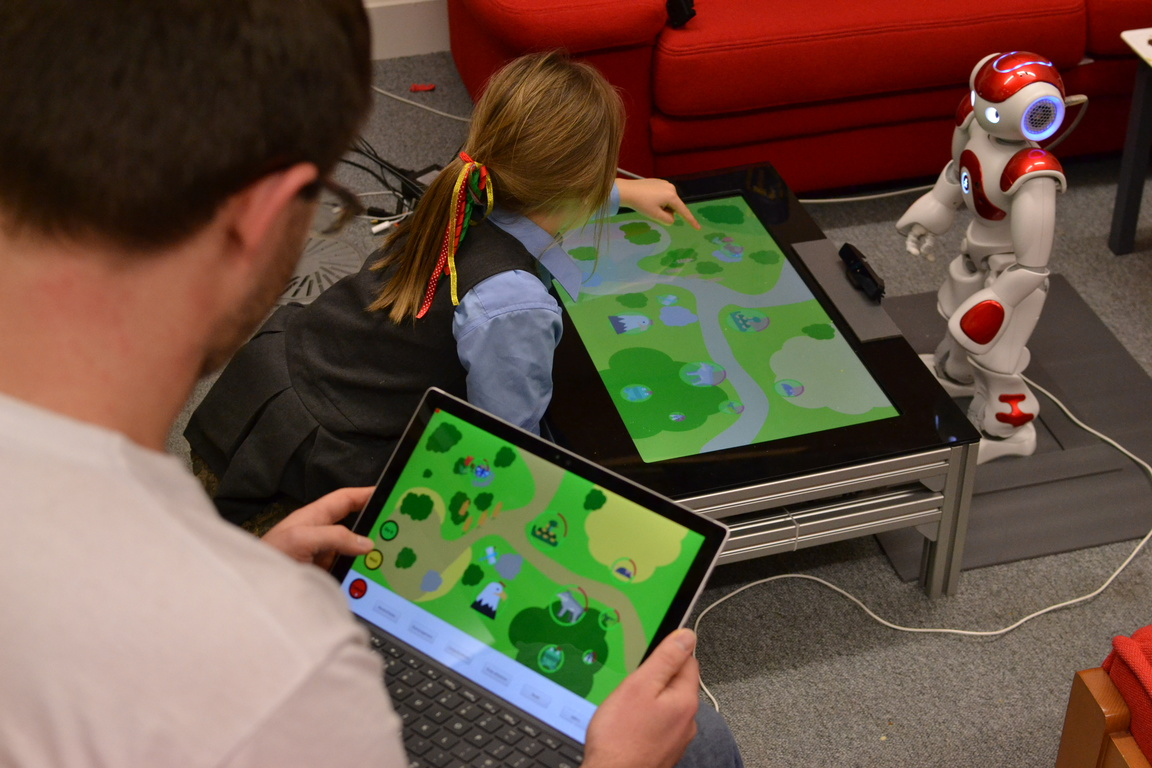
\includegraphics[width=.5\textwidth]{setup.jpg}
	\caption{Setup used in the study: a child interacts with the robot tutor, with a large touchscreen sitting between them displaying the learning activity; a human teacher provides supervision to the robot through a tablet and monitors the robot learning.}
	\label{fig:tutoring_setup}
\end{figure}

By interacting with the robot and the sandtray, the child is expected to gain knowledge on a specific topic. For this study, the task is learning about food chains by exploring a specific food web (interconnections between multiple food chains) in an educative game. The child plays a game on the sandtray where they can move animals to discover the interactions between them. Learning is evaluated by a test before, between and after the sessions; and the robot guides the child through the study and can, depending of the condition, support them during the game.

\subsection{Food Chain Game}

The main learning activity to teach the child the food web is a game composed of ten animals and three types of plants. Animals have energy decreasing over time and they have to eat to stay healthy. Animals are not moving unless the child or the robot moves them and can eat or be eaten when entering in contact with another animal or a plant. The child has to feed the animals by moving them to their food to give them more energy and by feeding the animals, children should learn the animals' diet. Figure~\ref{fig:tutoring_game} presents an example of the game screen in the middle of a session.

\begin{figure}[ht]
	\centering
		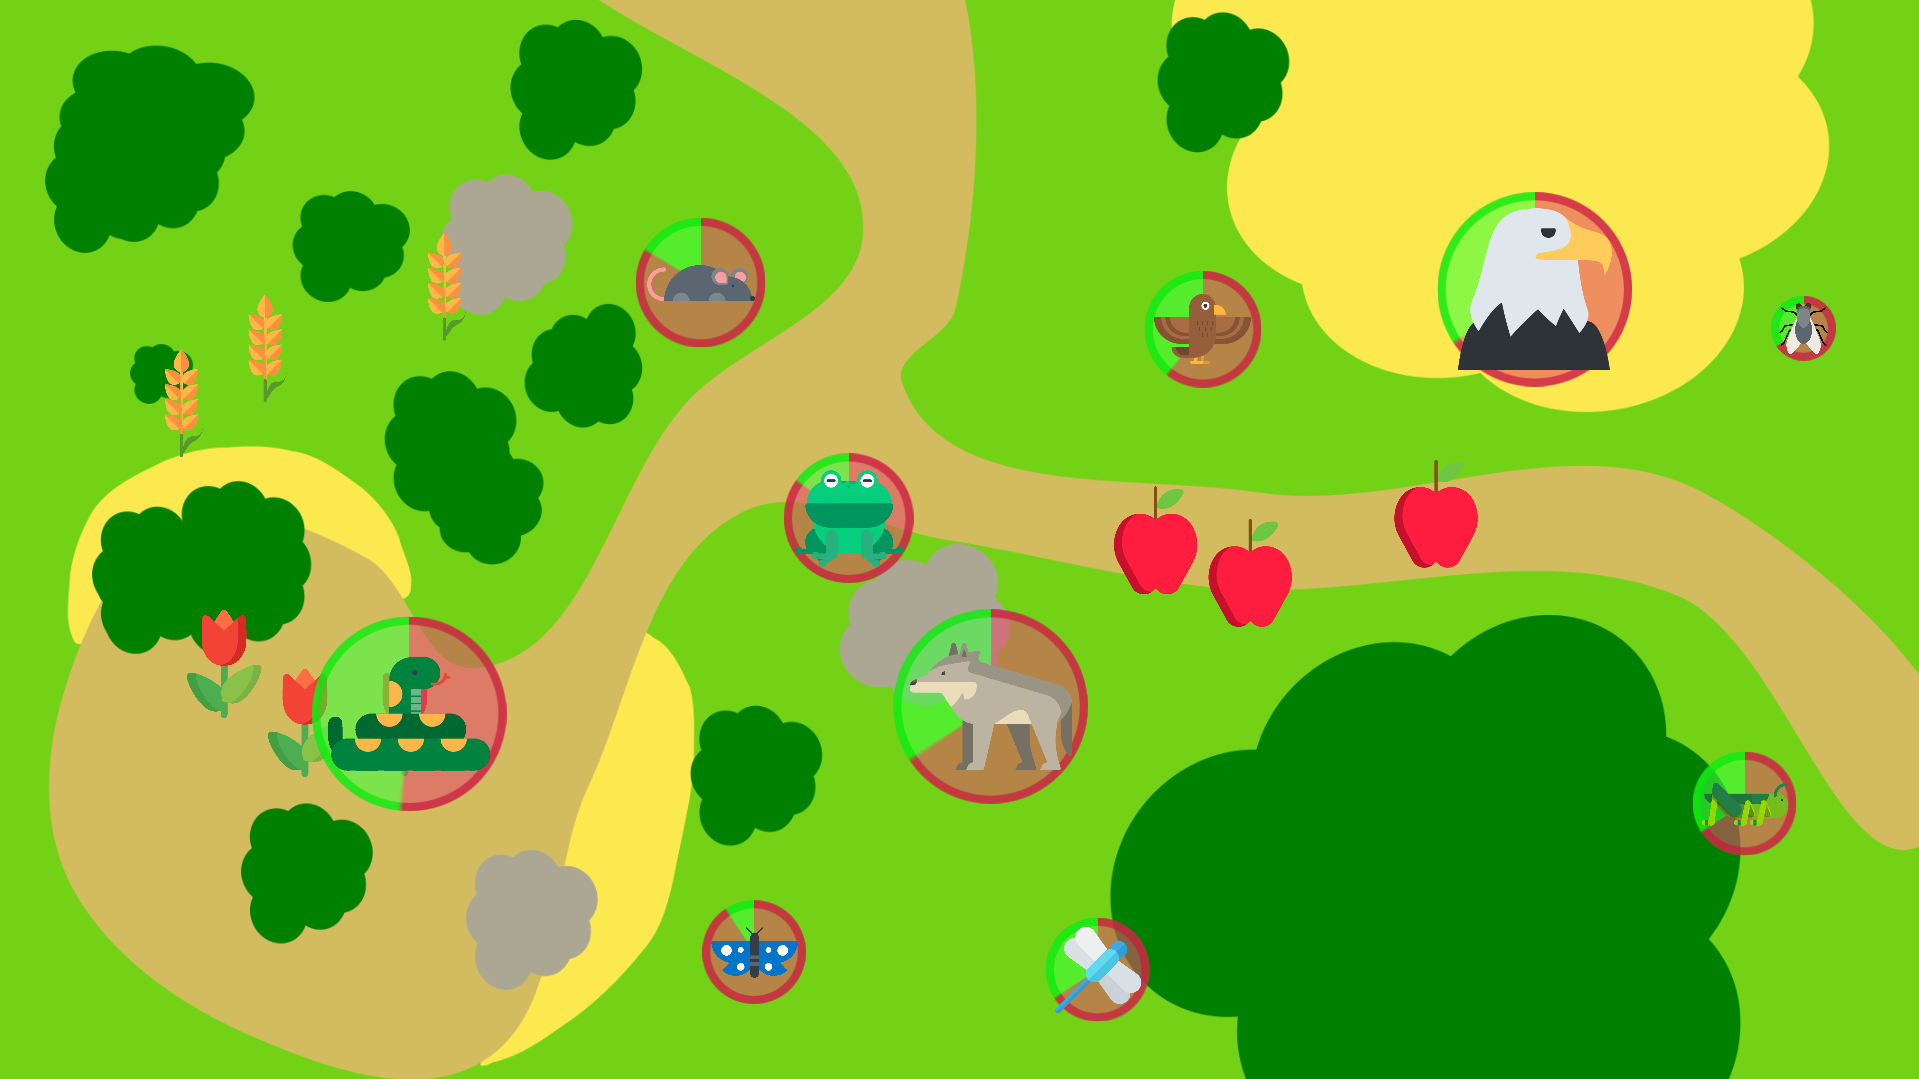
\includegraphics[width=1\textwidth]{game.png}
		\captionsetup{width=.9\linewidth}
		\caption{Example of the game. Animals have energy in green and have to eat plants or other animals to survive. The child's task is to keep animals alive as long as possible.}
		\label{fig:tutoring_game}
\end{figure}

\subsection{Robot Behaviour}
 
During the game, the robot can execute actions to provide hints and support to the child. The robot has access to five types of actions:
\begin{itemize}
	\item Movements: moving any animal to, toward or away from any items (animal or plant) - the robot points to an animal and moves it on the game while describing its action (e.g. "The eagle needs help getting close to the mouse").
	\item Drawing attention: the robot points an item and says a reminder to the child (e.g. "Don't forget the frog").
	\item Reminding rules: the robot says one of 5 sentences describing the game's rules (e.g. "Move the animals to feed them" or "Feed animals with a low energy").
	\item Congratulation: the robot provides congratulations (e.g. "Well done").
	\item Encouragement: the robot provides encouragement (e.g. "You can do it").
\end{itemize}
Considering all the possible combinations of actions and items, the total number of actions adds up 655. Additionally, to prevent the robot's behaviour to be repetitive and annoying, each utterance joining an action has multiple versions, and a random one not used recently is selected. 

This set of actions has been selected to be generalisable to many type of scenario including a teaching activity on a screen. Furthermore, in this study, these actions represent different level of support, from general motivation and information on the game's goal to which animals the child should focus on or direct information about what an animal eats. This selection of actions aims to cover a large range of possible tutoring behaviours humans could use. 

\subsection{Wizard of Oz Application}

In this study, the communication between the teacher and the robot occurs through the \gls{woz} application, a \gls{gui} running on a tablet and allowing the teacher and the robot to communicate. This \gls{gui} represents the state of the game as the child sees it, but with additional button and functionalities to communicate both ways with the robot (see Figure~\ref{fig:tutoring_gui}). The teacher can use a combination of buttons and moving animals on the tablet to have the robot execute any possible action. For example, to move animals close to another item, the teacher can drag and release the animal's image to a position to request the robot to execute this movement. The robot controller will infer which action has been selected by the teacher by evaluating how the distances between animals change. Additionally, the teacher can select other animals or plants to clarify their action and give information to the learning algorithm about what features were relevant in the decision process. Similarly, the teacher can select an animal and press the `Draw attention' button to have the robot point at the select animal and remind the child to use it.
%The main aim of the study being testing \gls{sparc} in a real \gls{hri}, the teacher needs an interface to communicate with the robot. To allow this interaction between the teacher and the robot, a \gls{gui} running on a tablet has been developed representing the current state of the game exactly as the child sees it on the touchscreen (see in Figure~\ref{fig:tutoring_gui}). This \gls{gui} runs on a tablet as it allow the robot's teacher to supervise and teach the robot while monitoring the application interaction (i.e. the interaction between the child and the robot). Buttons for the actions (excluding movements) allow the teacher to select which action the want the robot to execute. The teacher can also have the robot move animals simply by dragging and releasing animals' images on the tablet. The teacher can also select animals or plants to specify which action they intend to do. 
For instance, by clicking on the frog and the `Draw attention' button, the robot will execute the \textit{drawing attention to the frog} action. 
%Similarly, the moving action require two items: the animal moved and the target of the motion. By selecting a target before moving an animal, the teacher can be sure that the robot interpret the action correctly. 
This \gls{gui} design gives access to the teacher to the full 655 actions without requiring as many buttons. %Additionally, the selection of items is used by the robot controller to identify the relevant features to transmit to the algorithm for the learning.


\begin{figure}[ht]
	\centering
	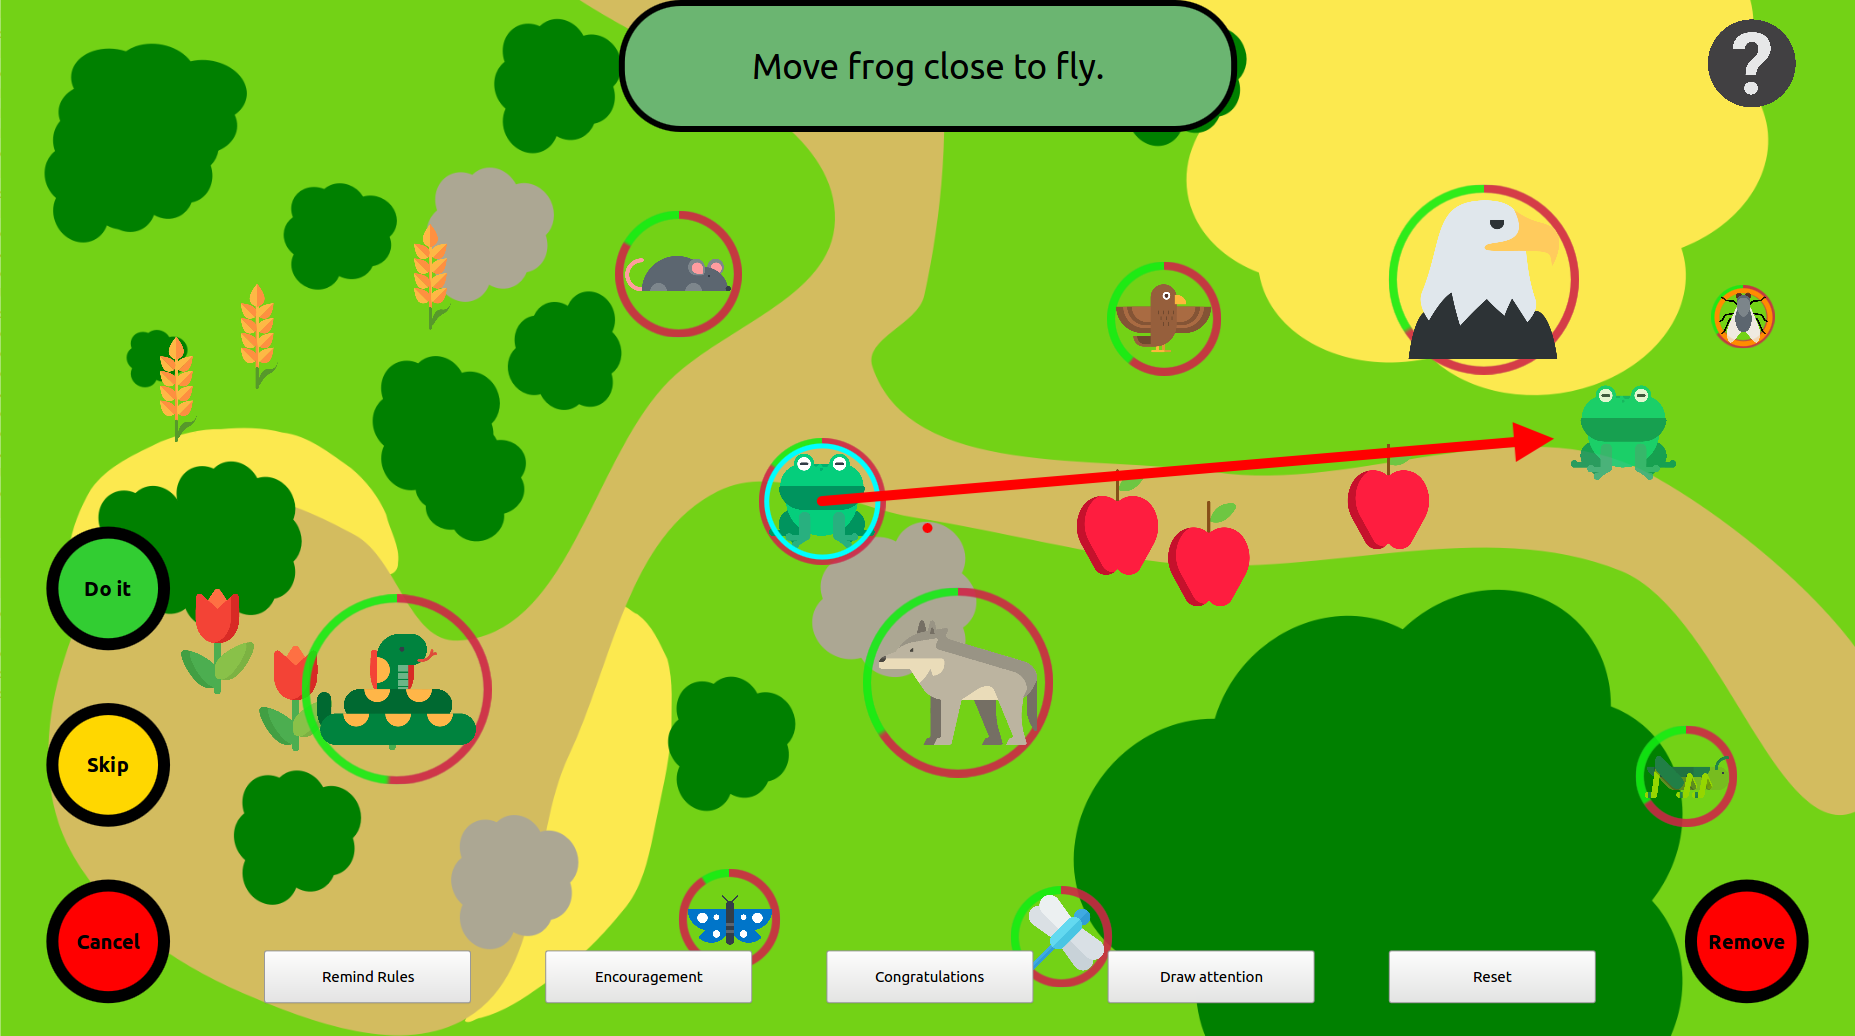
\includegraphics[width=1\textwidth]{gui.png}
	\captionsetup{width=.9\linewidth}
	\caption{\gls{gui} used by the teacher to control the robot and respond to its suggestions. The game is in the same state as in Figure~\ref{fig:tutoring_game}, and the robot proposes to move the frog close to the fly (text bubble, arrow, moving the \textit{shadow} of the frog and highlight the frog and the fly).}
	\label{fig:tutoring_gui}
\end{figure}


Finally, the \gls{gui} is also used by the teacher to respond to the robot's propositions. Following the proposition of an action, a bubble describing the action will appear on top of the \gls{gui}, the corresponding items will be highlighted and if the action is a motion, an arrow will show the proposed motion. The teacher can react to the proposed action by pressing the `Do it', `Skip', `Cancel' or `Remove' buttons or let the action be executed. The action will be automatically executed after 2 seconds, during which the bubble will become greener to represent the passive acceptance of the action. The `Do it' button executes the action straight-away, the `Skip' button informs the algorithm that it should wait rather than doing the action, the `Cancel' button assigns a negative reward to this action in that state and finally, the `Remove' button looks for the closest previous instantiation of the action in memory and removes it, preventing this instance to be used in later action selection.

\subsection{Algorithm}

The learning algorithm aims to reproduce the action policy by mapping an action (or no action) to each possible state. The state used in this study represents the situation of the game in a 210 dimensional vector, with continuous values from 0 to 1. The dimensions include: distance between items, items' energy, progression in the game sessions, child face direction (toward the robot, the screen or away) and time since events (child and robot touching each animal, robot's actions, interaction events: feeding an animal, death of an animal...). As mentioned before, the action space covers moving items in relation to other items, drawing attention to items, providing encouragements, congratulations and reminding the rules. In summary, the algorithm's task is to map an action from the 655 (including a `wait' action) to each possible combination on the 210-dimension state. A more detailed definition of the state space can be found in Appendix~\ref{ann:state} and Appendix~\ref{ann:action} for the action space.

The actions and the state dimensions have been selected to be generic to many teaching tasks involving movable items: each item has a value assigned to it (here energy, but this could be changed in other scenario), and some movable items (here animals) can be move to, toward or away from other items. Using these generic actions and this state definition, this implementation could be easily re-purposed to another teaching task.

The algorithm used for the learning is an adaptation of the one presented in \cite{senft2017toward}. It is an instance based algorithm similar to the nearest-neighbours algorithm~\citep{cover1967nearest}. However, two differences are notable compared to the initial algorithm. %: instances are defined on a sliced part of the state and each instance instance is associated to a reward defining the interest of the agent to select this action in that state.
Firstly, instead of being defined on the full state space, instances are defined on a sliced version of the state. The intuition is that states needed to cover complex action policies require large number of dimensions, however for each single action, large parts of the state are irrelevant. For example, if a robot needs to pick-up a cup, the colour of the cup does not impact the optimal motion. In contrast, the colour matters if the robot has to answer the question: ``which cup is on the left? The blue one or the red one?''. Consequently, the colour of the cup should be part of the state space, but should not be considered when selecting some of the actions. For this implementation, when selecting actions, the teacher can highlight features of the environment which \emph{activates} specific dimensions of the state space which are used to store the instance in memory. By default, all the generic events (death, feeding, failed interaction) and time since the last child and robot actions are \emph{activated}. All the \emph{non-activated} dimensions are left as wild-cards. Then, when comparing the current state to the saved instances, the distance is only computed on the \emph{activated} dimensions of the stored instance. The second difference is that each instance saved has a reward assigned to it. For this study, if the teacher selects the action, the \gls{gui} assigns a reward of $+1$, and if the teacher cancels the action (following an incorrect suggestion from the algorithm) the reward is $-1$. When selecting an action, the algorithm looks through all the actions it has been using and for each action selects the closest instance to the current state and computes the expected reward as a multiplication of the distance by the reward. Then the algorithm selects the action with the highest expected reward and proposes it to the teacher if the value is higher than an adaptive threshold (cf. Algorithm~\ref{algo:tuto}). 

\begin{algorithm}
	\DontPrintSemicolon
	\SetKwInOut{Input}{inputs}\SetKwInOut{Output}{output}
	\Input{$s$: current state, C: collection of  $(a,s',r)$}
	\Output{selected action $\pi(s)$}
	\ForEach{$a \in A$}{
		\ForEach{$p=(s',r) \in C_{a}$}{
			compute similarity $\Delta$ between $s$ and $s'$:
			$\Delta(p)=1-\frac{\sum_{i}^{n'}(s'(i)-s(i))^{2}}{n'}$
		}
		find closest pair $\hat{p}$:\\
		$\hat{p} = arg\, max_{p} \Delta(p)$\\
		compute expected reward $\hat{r}(a)$ for taking $a$ in $s$:\\
		$\hat{r}(a) = \Delta (\hat{p}) \cdot r(\hat{p})$\\
		with $r(p)$ the reward $r$ of the pair $p = (s',r)$ 
	}
	Select the action with the maximum expected reward:
	$\pi(s) = arg\, max_{a} \hat{r}(a)$
	
	\If{$\hat{r}(\pi(s)) >$ threshold}{
		Propose $\pi(s)$ to supervisor
	}
	
	\caption{Algorithm for selecting an action based on the previous instances tuples (partial state, action, reward) and the current state. Partial states are defined on a subset of the state space with n' active dimensions.}
	\label{algo:tuto}
\end{algorithm}

The algorithm runs at 2Hz while we would expect actions to be selected every 5 to 20 seconds. So, unlike most of the discrete cases of action selection, in most of the steps no action should be executed. To handle this difference of timescale, a waiting action has been added (through the `Skip' button) and an adaptive threshold limits the propositions to actions with a high expected reward. When receiving an action with a positive reward, if the threshold is higher than the previous maximum similarity between this action's instances and the current state, the threshold would be decreased and this effect is inverted for negative rewards. Selecting an action can reduce the threshold, and cancelling or skipping an action can increase it. This aims to adapt the rate of action proposition to the desires of the teacher. A last mechanism filters propositions from the algorithm not to transfer them to the teacher when an action is already proposed or the robot is currently acting. This filter also rewards negatively impossible actions (such as moving dead animals).

\subsection{Study Design}

%Parents completed a consent form and each child was proposed to withdraw if they appeared not interested to continue the study (children refusing to continue have been replaced to reach the same number in each category). 
The interaction protocol was as follows. Children were first introduced to the robot and the aim of the interaction and then had a first pre-test to evaluate their initial knowledge. Before starting the teaching game, children had to complete a tutorial where they were introduced to the mechanics of the game: animals have life and have to eat to survive and children can move animals to make them interact with other animals or plants and replenish their energy. After this short tutorial, they completed two sessions of the game where the robot could provide feedback and advices depending on the conditions they were in. Following these initial sessions of the game, children completed a mid-test before playing another 2 sessions of the game and a last post-test to conclude the study. 

%\begin{figure}[h]
%	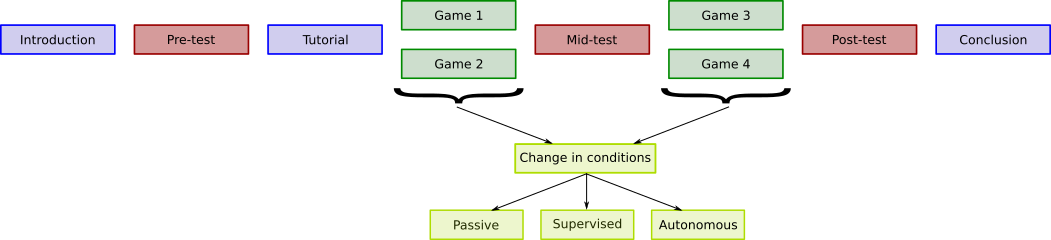
\includegraphics[width=.9\linewidth]{graph.png}
%	\centering
%	\caption{Methodology used for the study.}
%	\label{fig:method}
%\end{figure}

The study evaluated three conditions: the passive condition, supervised condition and autonomous condition. In all the conditions, the robot's behaviour during the introduction, tests, tutorial and conclusion was identical. The only change of behaviour happened during the games sessions. The study design was between participants, so children were each assigned to a condition, and in all the game session, the robot would be passive, supervised or autonomous. %In the passive condition, the robot does not provide support during the game. In the supervised condition, the robot is controlled by a PhD student in psychology acting as the robot's teacher and demonstrating it how to interact. And in the autonomous condition, the robot simply applies the learned policy without supervision.

In the \textit{Passive} condition, the robot did not provide any advice nor feedback to the children during the game sessions. It only oscillated slightly to simulate a breathing motion and followed the child's face. In the \textit{Supervised} condition, the robot was remotely supervised by an operator using \gls{sparc}. Finally, in the \textit{Autonomous} condition, the robot applied the learnt policy and provided feedback and guidance to the child without human supervision.

In the study, the teacher was a psychology PhD student from the university, with limited knowledge in computing and machine learning. She had been instructed how to control the robot using the GUI, the effect of each buttons and how to perform each action. She was knowledgeable of the methodology used to run the study (but not the underlying implementation) and experimented controlling the robot in two interactions with the author interacting with the robot and one with a child before starting to supervise the robot for the supervised condition. No information about the learning algorithm or the representation of the state and no feedback about optimal way of interacting or feedback on her action policy was provided before or during the supervision. As such, this robot teacher represents typical target populations for robotic applications: non-experts in machine learning or computing but with relevant domain knowledge such as teachers or psychologists.

In the autonomous condition, the robot used the suggestions from the algorithm and executed them with a probabilistic delay between 0 and 1.5 seconds based on the teacher's delay in answering the robot's propositions. This delay aimed to give a pace and synchronisation of actions similar to the ones exhibited by the teacher when reacting to the robot's suggestion.

% Figure~\ref{fig:tutoring_game} shows an example of the game screen. The child can move 10 animals across the game field and can have them interact with other animals or plants. Animals lose energy over time and by interacting with their food the can regain some. Animals that are eaten lose a chunk of their life. The goal for the children is to keep animals alive as long as possible by feeding them and they earn stars representing how healthy their animals have been during the session. The game stops when 3 or more animals run out of energy and each game session lasted 1.6 minutes in average.

\subsection{Metrics}

%Redundant with hypothese?
%This study aimed mostly at evaluating if \gls{sparc} allows a human non-expert in computing to teach a robot from in-situ supervision. 
%This teaching capability is divided into three parts: 
%\begin{itemize}
%	\item How similar the teacher's and autonomous robot's policies are? 
%	\item What are the impacts of the active robot on the child behaviour? \\(And what are the differences between the autonomous and supervised robots?)
%	\item How the online learning component changed the interaction between the robot and the teacher?
%\end{itemize}

To address the hypotheses presented in Section~\ref{sec:tutoring_scope}, we collected multiple metrics on both interactions (teaching and application). First, we recorded the actions executed by the robot in the supervised and autonomous conditions to characterise the two action policies. Two groups of metrics have been collected to evaluate the application interaction: the learning metrics (corresponding to children's performance during the test) and the game metrics (corresponding to children's behaviour during the game). And finally, in the supervised condition, we recorded the origin of the action executed by the robot (teacher vs algorithm) and the outcome of the proposed actions (executed vs refused).

\subsubsection{Policy Characterisation}

During the game, the robot had access to 622 actions, which can be divided in seven categories: drawing attention, moving close, moving away, moving to, congatulation, encouragements and reminding rules. Due to this high number of actions, the largeness of the state space (210 dimension) and the complex interdependence between actions and states, totally defining a policy is impossible. Consequently, we decided to use the number of actions executed for each category per child to characterise the policy executed by the robot in the active conditions (supervised and autonomous). While not perfectly representing the action policy of each condition (e.g. the timing of actions is missing), this metric offers a proxy to compare these policies. 

\subsubsection{Learning Evaluation}
The learning was evaluated through an open graph where children had to connect animals to their food. Figure~\ref{fig:test} shows two examples of the test, with or without all the correct connections. Children were instructed to connect as many animals as possible. During the pre-test, the experimenter demonstrated how to connect animals by drawing an arrow from the frog to the fly, and then removing the arrow by pressing the \textit{X} button. When children thought they were done, they could press the `Continue' button, showing a screen asking confirmation to quit the test or allowing children to keep connecting animals. Additionally, the robot informed the child if not all the animals were connected to a food or that animals could eat many types of food if no more than one animal was connected to two items. 

\begin{figure*}[ht]
	\centering
	\begin{subfigure}[t]{0.5\textwidth}
		\centering
		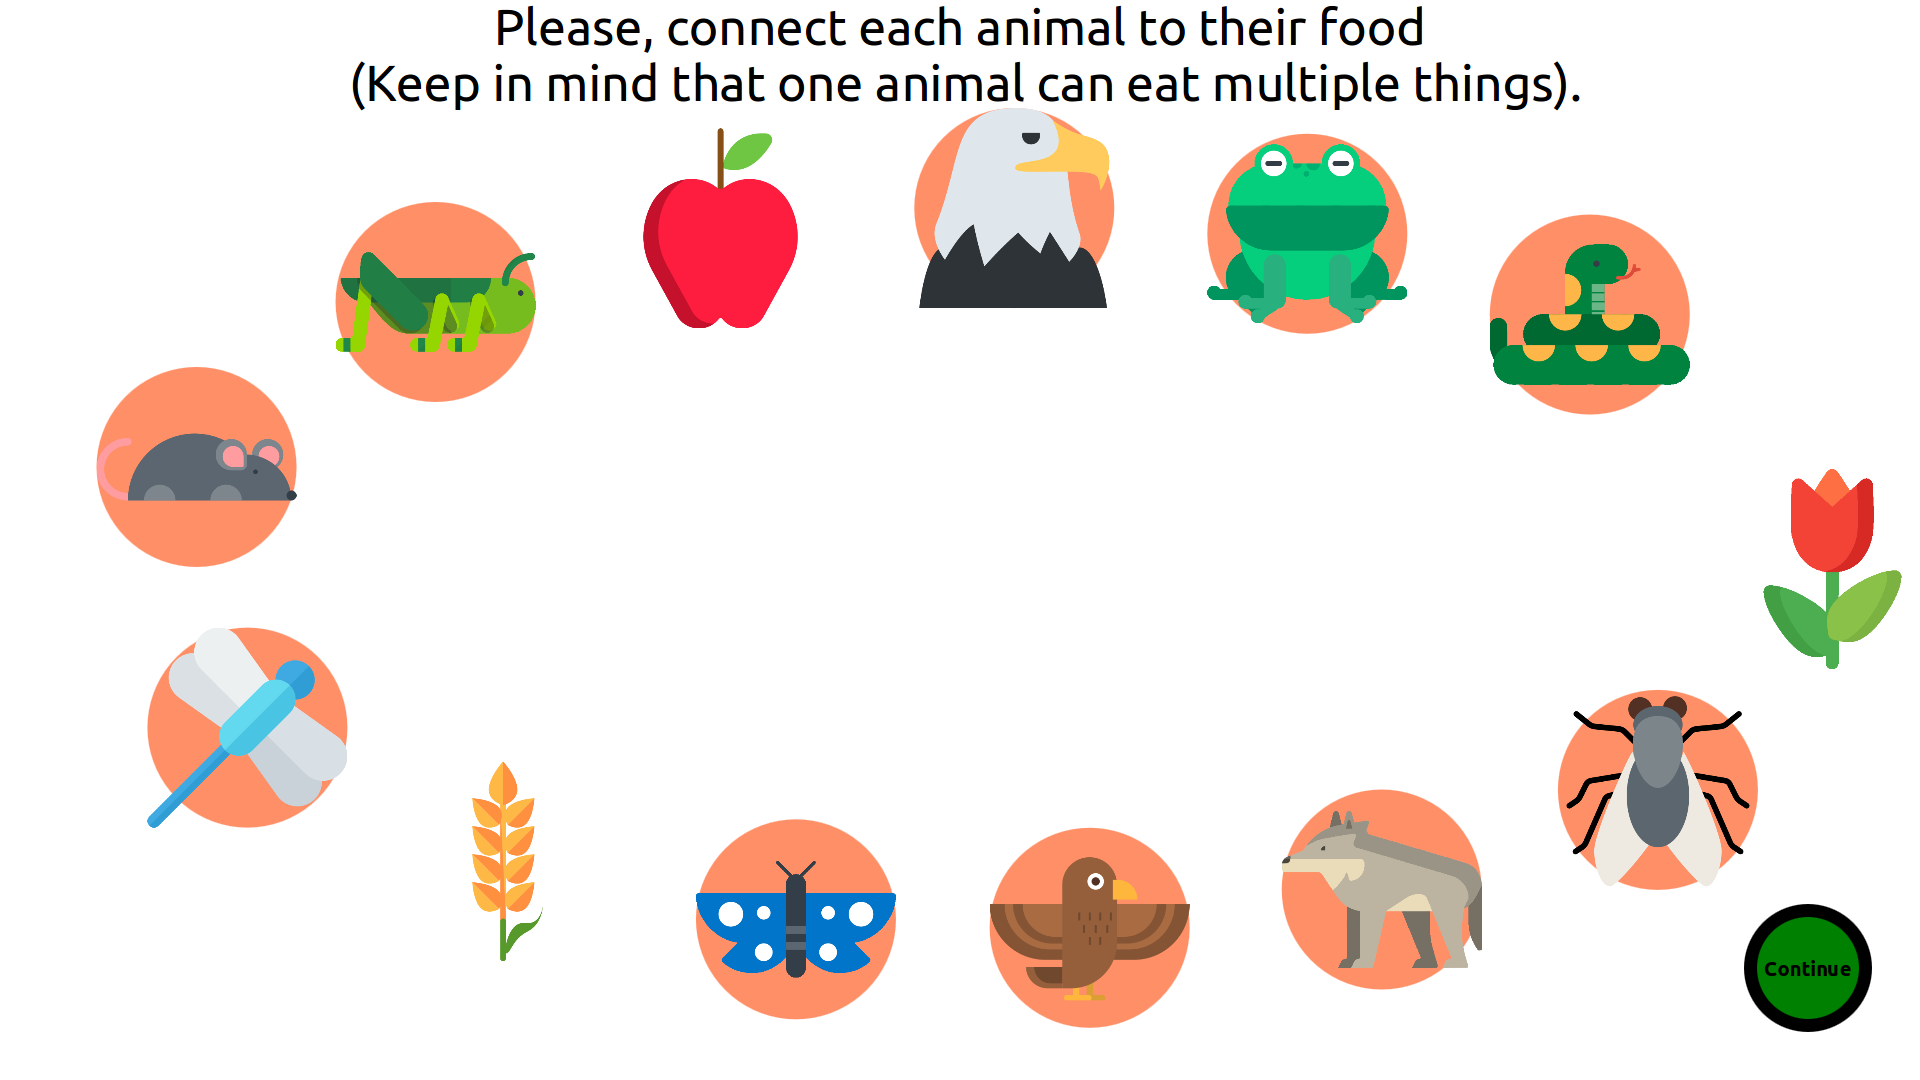
\includegraphics[width=0.95\textwidth]{empty_graph.png}
		\captionsetup{width=.95\linewidth}
		\caption{Empty screen that children face at each test. Red dots behind animals indicate that they are not connected to any food.}
	\end{subfigure}%
	~ 
	\begin{subfigure}[t]{0.5\textwidth}
		\centering
		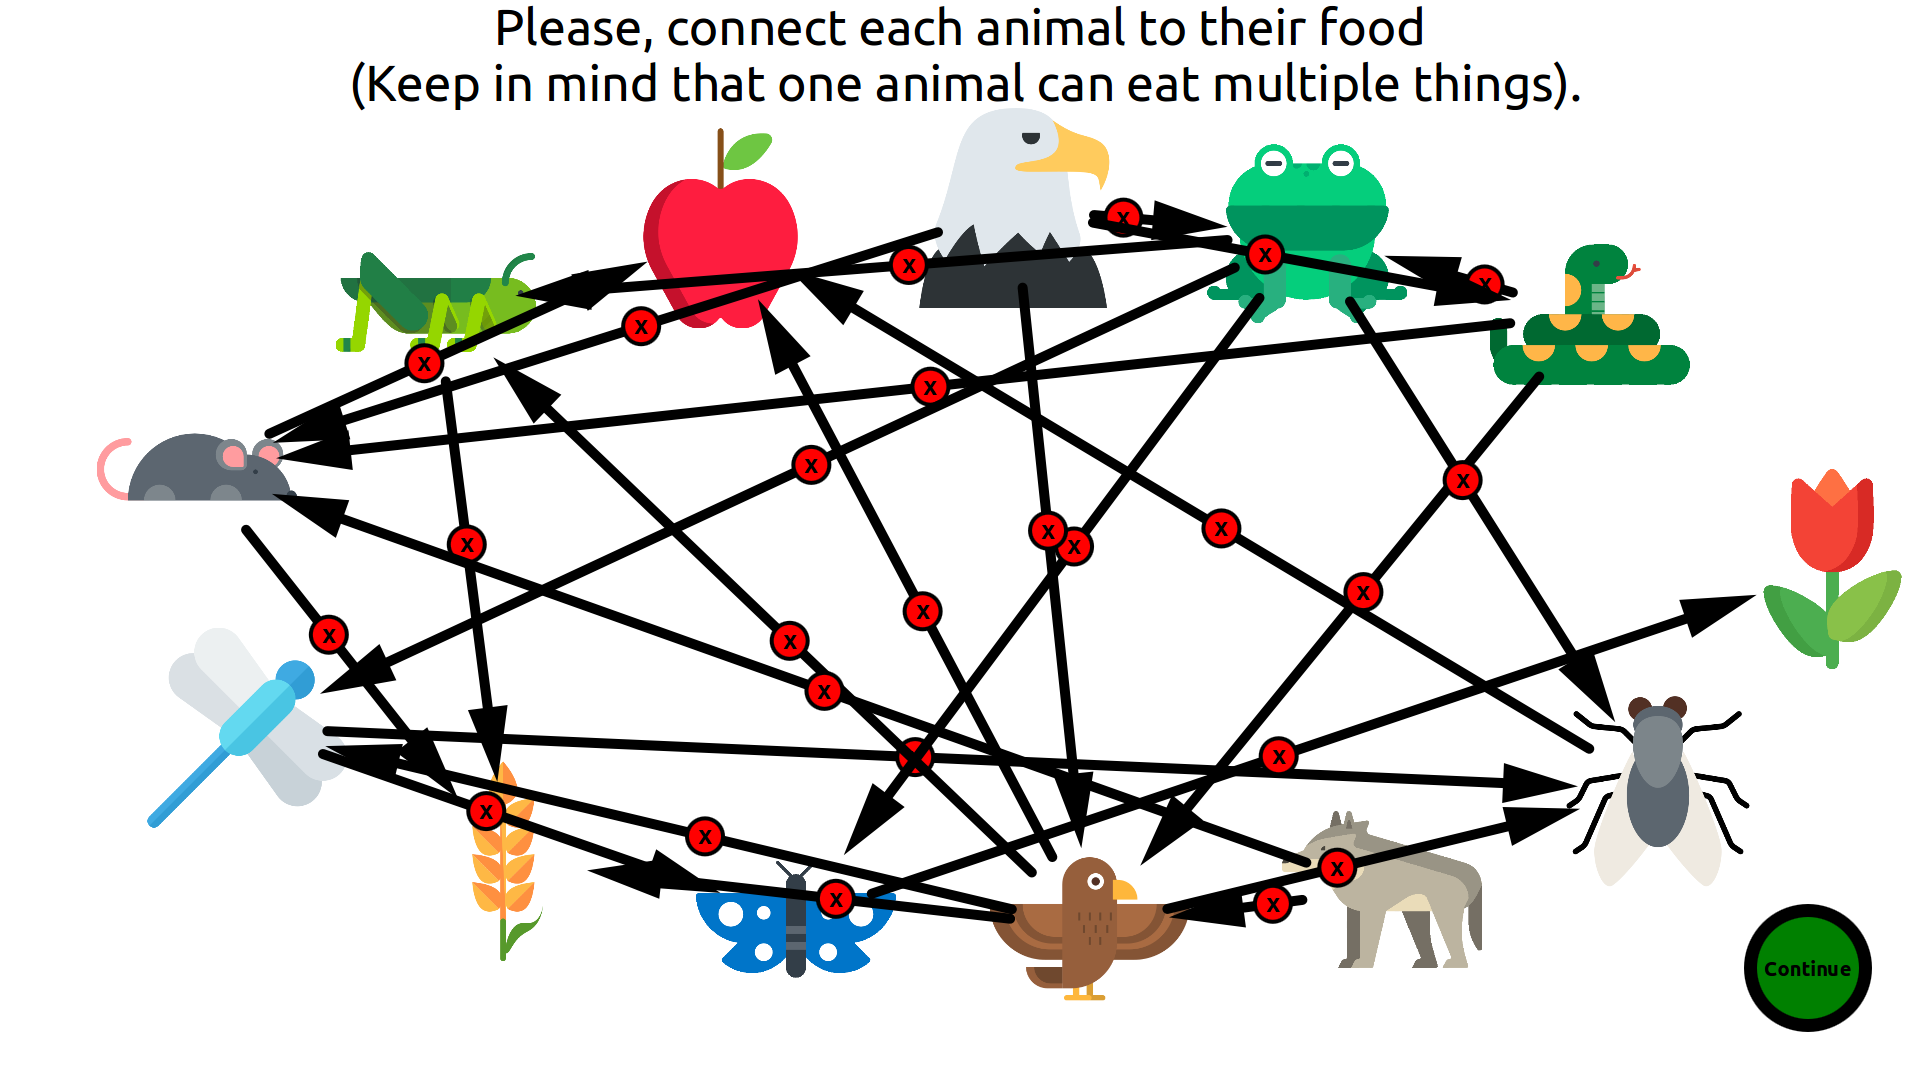
\includegraphics[width=0.95\textwidth]{full_graph.png}
		\captionsetup{width=.95\linewidth}
		\caption{Fully connected test with all the correct connections.}
	\end{subfigure}
	\caption{Test screen to evaluate children's knowledge, empty starting screen (a) and fully connected and correct test (b).}
	\label{fig:test}
\end{figure*}

They are in total 25 different correct connections and 95 possible incorrect ones. As the child can connect as many arrows as desired, the performance is defined as the number of correct arrows above chance (for the number of connected arrows on the test) divided by the maximum achievable performance to reach a score bounded to $[-1,1]$. For example, if a child connects 5 good arrows and 3 bad, their performance would be:

\begin{equation}
P=\frac{\#good-(\#good+\#bad) \cdot \frac{total good}{total}}{total good - total good \cdot \frac{total good}{total}} = \frac{5-(5+3) \cdot \frac{25}{25+95}}{25 - 25 \cdot \frac{25}{25+95}}=0.168
\end{equation}
			
The three tests (pre, mid and post interaction) result in three performance measures. To account with initial differences of knowledge and the progressive difficulty to gain additional knowledge, we computed the learning gain as the difference between the final and initial knowledge divided by the `progression margin': the difference between the maximum achievable performance and the initial performance. This learning gain indicates how much of the missing knowledge the child managed to gain from the game.
			
\subsubsection{Game Metrics}
Different metrics have been gathered during the game sessions to characterise the children's behaviours:
\begin{itemize}
	\item \textbf{Number of different eating interactions}: number of unique feeding action type.
	\item \textbf{Points}: cumulated sum of animals' energy over the game (typical range [550,1100]).
	\item \textbf{Interaction time}: Duration of game sessions, how long a game lasted until three animals ran out of energy (typical range [.5,3] minutes).
\end{itemize}

The number of different eating interactions informs on how many learning items the children have encountered in the games. A feeding interaction happens when an animal is moved to its food (or to a predator); and the number of different feeding interaction represents how many different unique correct connections the child been exposed to during the game (multiple feeding actions between the same animals would count only once). A game with a high number of different feeding represents a game where the child had the opportunity to learn many correct connections between animals. Consequently, by increasing this number, the children would be exposed to more learning items which should help them to perform better on the tests. Both the interaction time and the number of points reached in the game inform on the children's success in the task: keeping the animals alive as long as possible. 

%Maybe talk about compliance

\subsubsection{Robot Learning}

In the supervised condition, the robot executed actions selected or validated by the teacher, and by using \gls{sparc}, the robot could propose actions to the teacher. Faced with a proposition, the teacher had multiple ways to react. They could accept the action (by waiting for it to be executed, pressing `Do it' or selecting the same action manually) or refuse it (by pressing the `Cancel', `Skip' or `Remove' buttons). As such, actions going through this pipeline can be divided in three categories: actions selected by the supervisor, robot's good propositions and robot's bad propositions. And the evolution of these categories represents how much the online component of the learning improved the quality of the robot's suggestions and reduced the workload on the teacher. 

Some times the teacher cancelled actions and then selected them again, we called this effect the `reselection'. To obtain the final numbers of accepted and refused actions, we removed these reselection from the bad propositions and we added them to the good propositions as it represents cases where the teacher refused an action by accident.

\section{Results}

% and right graphs present the 

%Preliminary results (currently in progress, due to be completed before the submission of the full article) show that (1) the robot is able to effectively jointly learn action and social policies (Figure 2), (2) the learning gains of the children supported by the autonomous robot are not significantly different from the gains when the learning is supported by a robot tele-operated by the human expert, which would indicate the utility of the approach.

Similarly to Chapter~\ref{chap:control}, we analysed the results using Bayesian statistics and the JASP software~\citep{jasp2018}. We used a Bayesian mixed ANOVA as omnibus test to explore the impact of conditions or repetition on the metrics. \ES{check how post hoc test}

\subsection{Comparison of Policy}

Figure~\ref{fig:tutoring_actions} presents the number of actions of each types executed by the teacher (in the supervised condition) and the autonomous robot. Both action policies presented similarities: the action `Move away' was almost never used, `Move to' was never used, and the supportive feedback (`Congratulation' and `Encouragement') were used more often than `Remind rules' or `Drawing attention'. However, some dissimilarities were also present, for instance, the autonomous robot used more encouragements than congratulations while the teacher did the opposite. The autonomous robot also reminded the rules more often and used the `Move close' action less than the supervisor. These differences of actions are probably linked to the type of machine learning used; with instance based learning, some datapoints will be used in the action selection much more often than others, which might explain these biases. But these results show that the robot managed to learn a social and technical action policy presenting similarities with the one displayed by the teacher providing partial support for H1.

\begin{figure}[ht]
	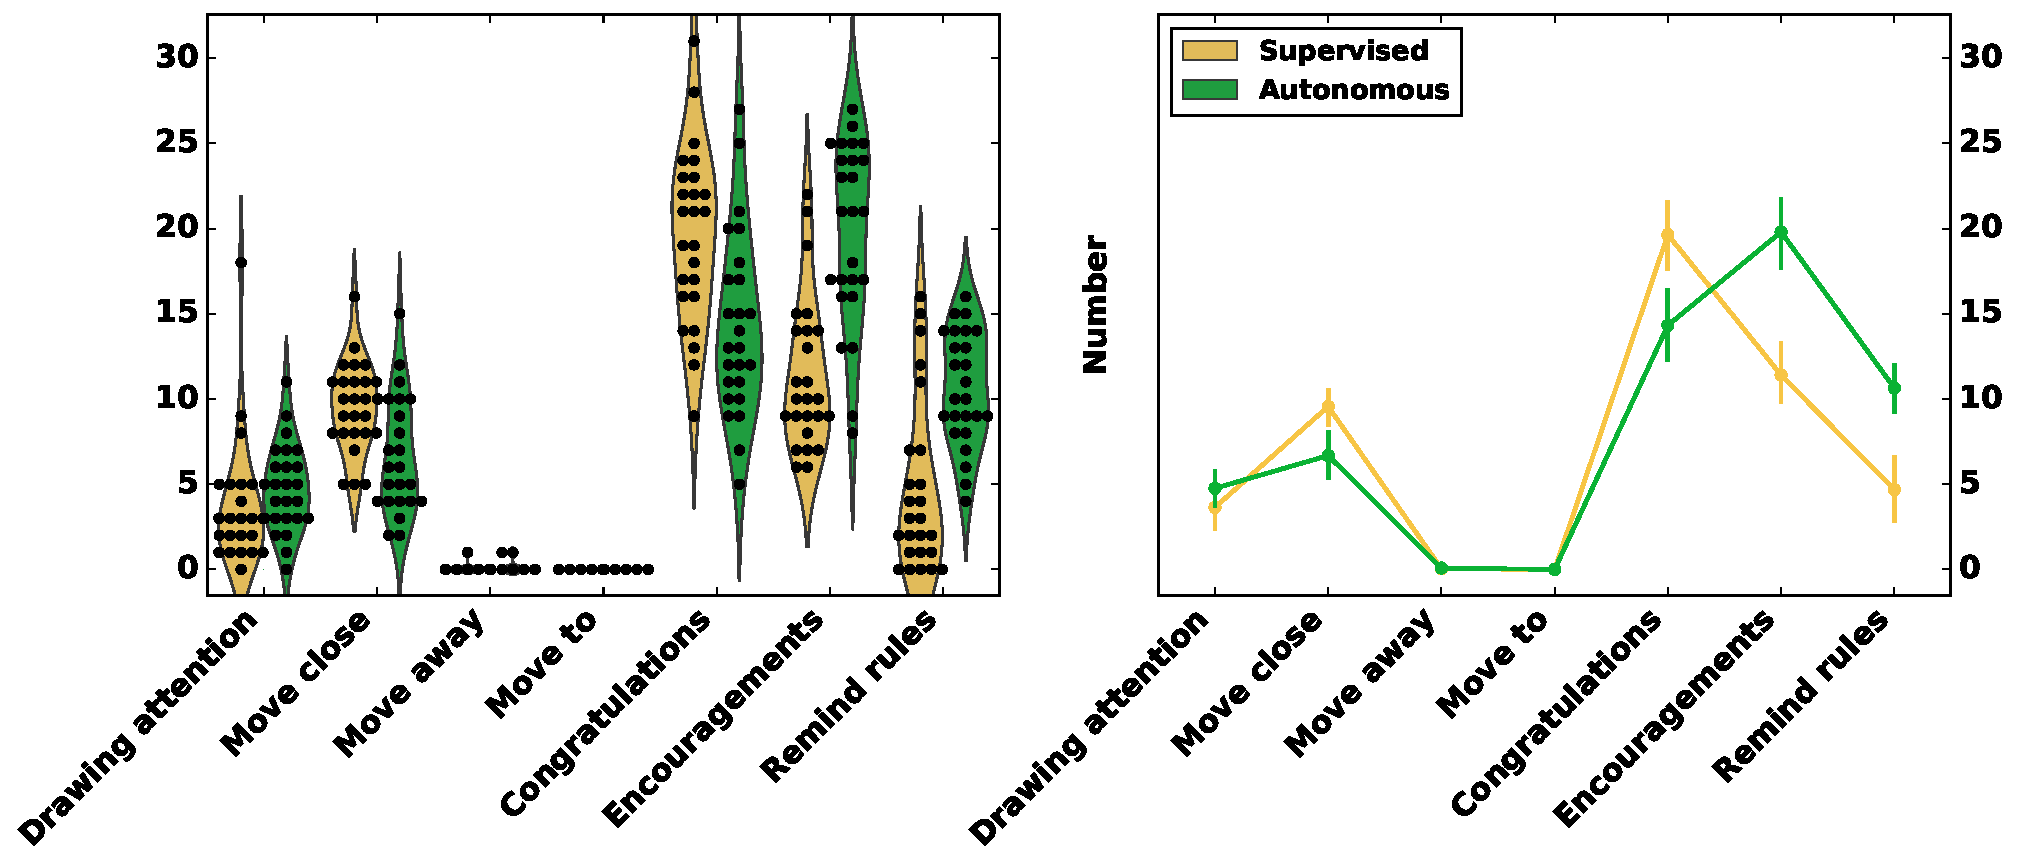
\includegraphics[width=1\linewidth]{actions.pdf}
	\centering
	\caption{Comparison of actions executed for the autonomous and supervised condition. The left graph is a violin plot of the data, while the right presents the means and the 95\% Confidence Intervals}
	\label{fig:tutoring_actions}
\end{figure}


%\begin{figure}[ht]
%	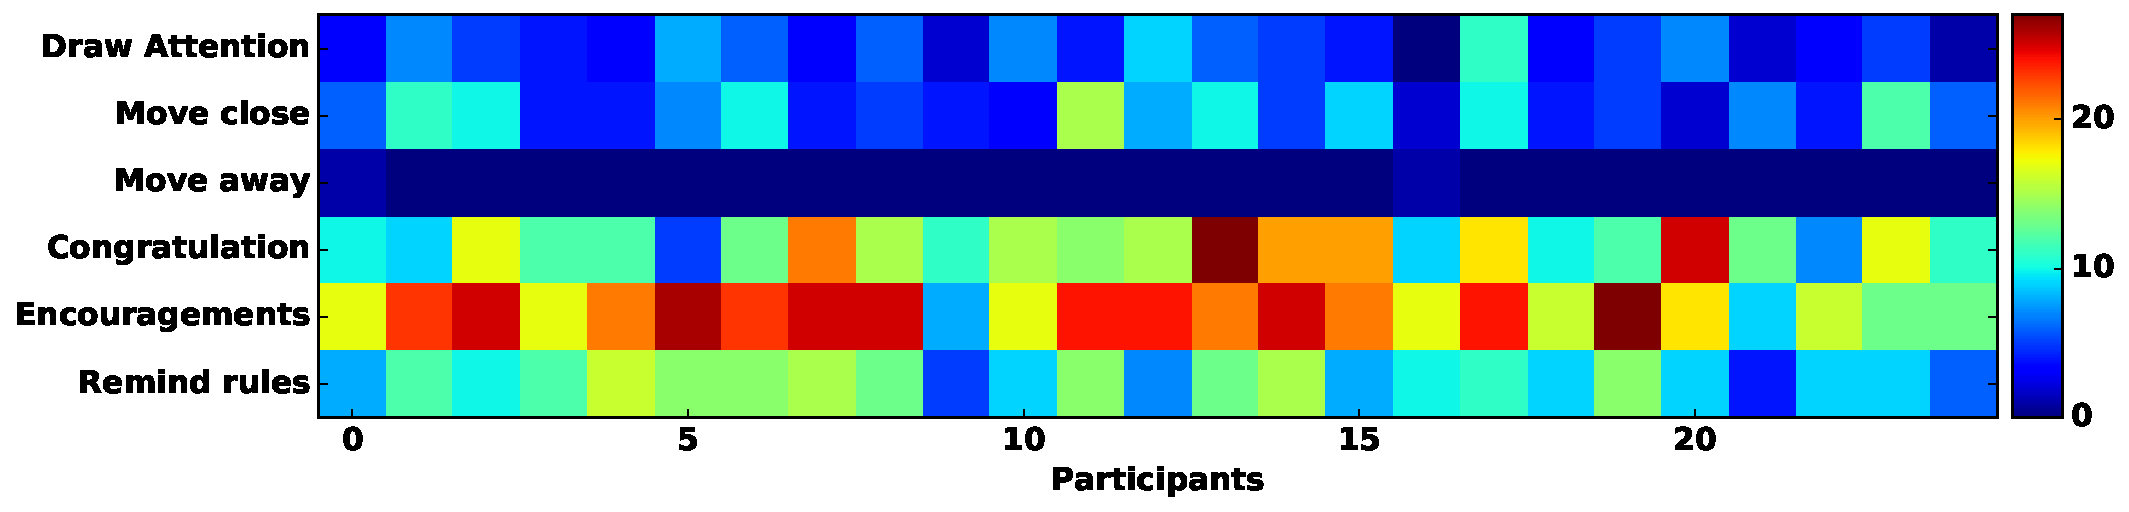
\includegraphics[width=1\linewidth]{autonomous_actions.pdf}
%	\centering
%	\caption{Repartition of actions across the participants in the autonomous condition.}
%	\label{fig:tutoring_autonomous_actions}
%\end{figure}
%
%\begin{table}[ht]
%	\centering
%	\caption{Repartition of action in the policy for both conditions (in \%).}
%	\label{tab:tutoring_policies}
%	\begin{tabularx}{\textwidth}{@{}lYYYccY}\toprule
%		& Draw \newline Attention & Move \newline close & Move \newline away & Congratulation & Encouragements & Remind \newline rules \\
%		\midrule
%		Supervised & 6.6  & 22.2 & 0.1 & 43.1 & 22.7 & 5.3 \\
%		Autonomous & 8.5 & 11.8 & 0.1 & 25.4 & 35.2 & 18.9\\
%		\bottomrule
%	\end{tabularx}
%\end{table}


\subsection{Test Performance}

Figure~\ref{fig:tutoring_performance} shows the evolution of children's performance across the three tests. A Bayesian mixed-ANOVA showed that in all conditions, children's performance increased across the tests ($B=1.5$x$10^{12}$), however the impact of the condition on the learning was inconclusive with a tendency to show no impact ($B=0.539$). This indicates that by being involved in the task, every children learned and improved their performances on the test (by gaining in average 13\% of the missing knowledge), but the robot behaviour during the game did not have an important impact on the children's learning gain (see Figure~\ref{fig:tutoring_learning}), invalidating H2.

\begin{figure}[ht]
	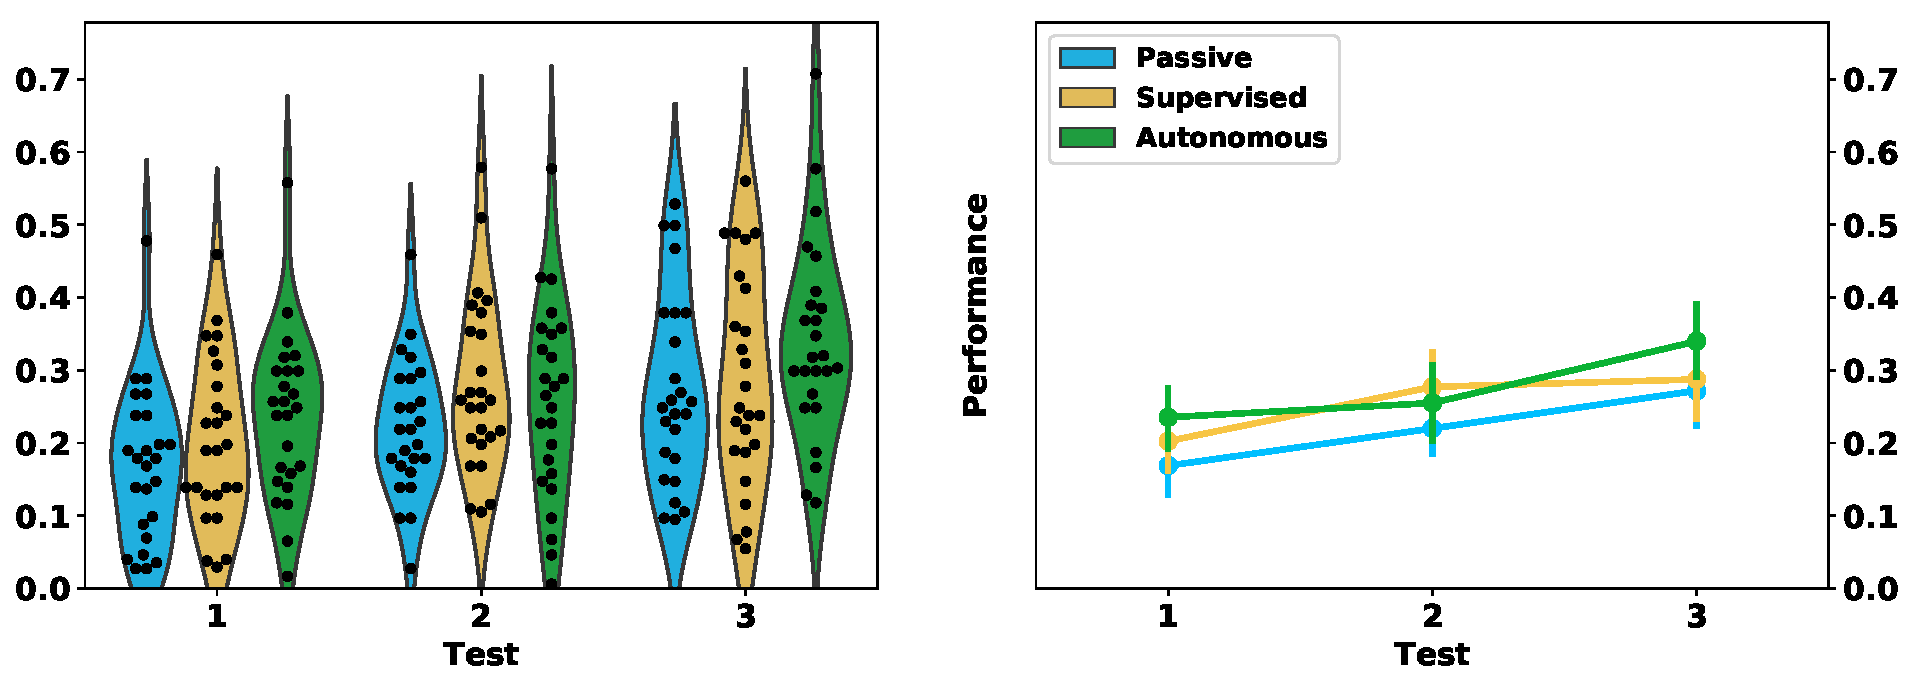
\includegraphics[width=1\linewidth]{perf.pdf}
	\centering
	\caption{Children's performance for the three tests: pretest, midtest and posttest for the three conditions.}
	\label{fig:tutoring_performance}
\end{figure}

\begin{figure}[ht]
	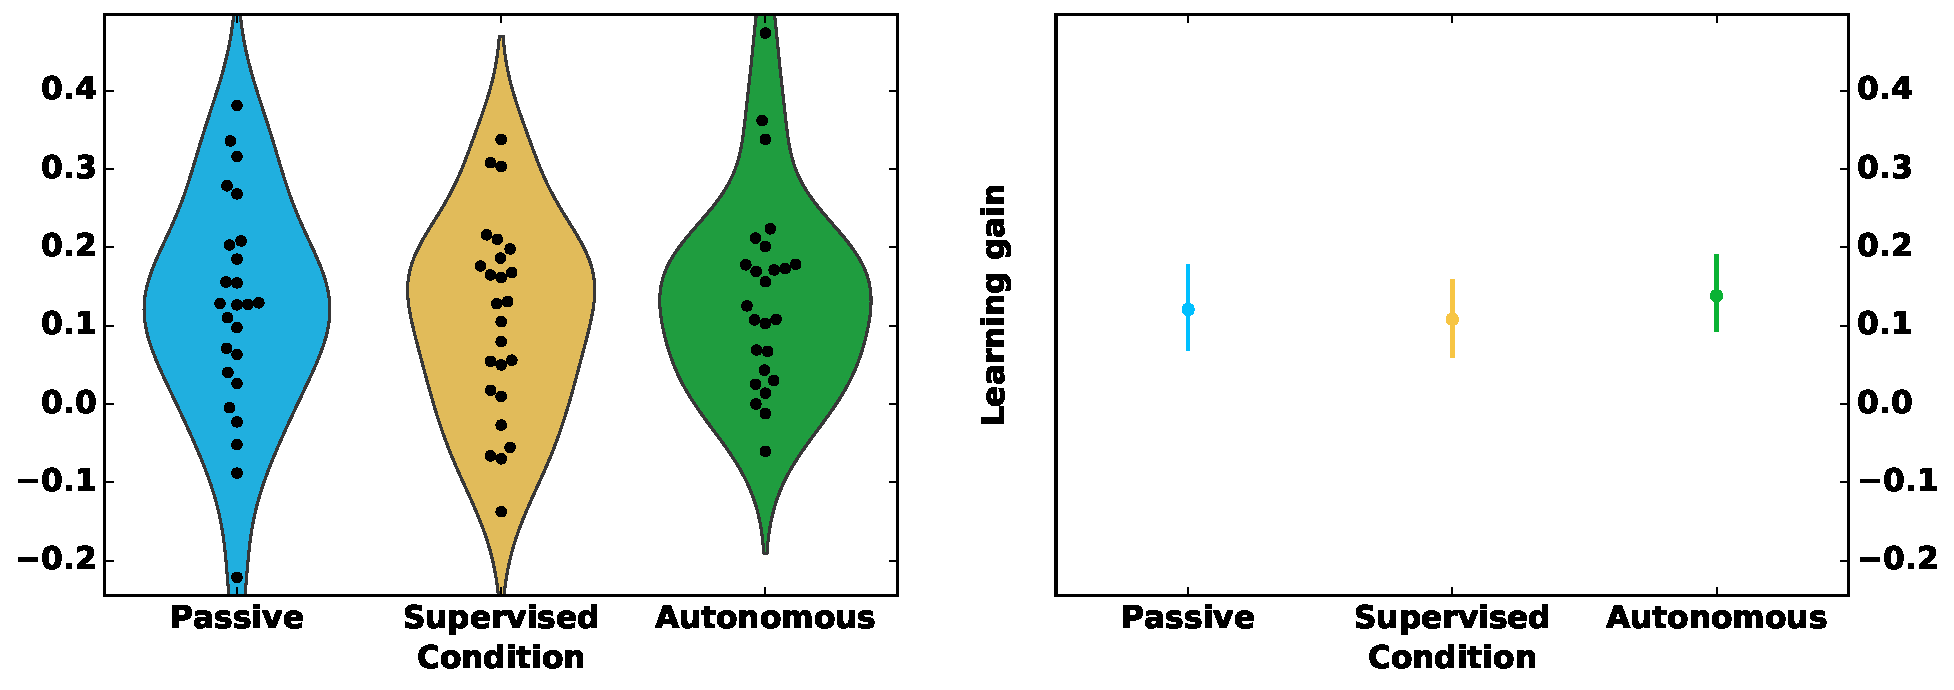
\includegraphics[width=1\linewidth]{learning.pdf}
	\centering
	\caption{Children's normalised learning gain after interacting with the robot for the three conditions.}
	\label{fig:tutoring_learning}
\end{figure}

\subsection{Game Metrics}

\paragraph{Different eating behaviours}
Figure~\ref{fig:tutoring_d_eat} shows the evolution of the number of different eating behaviours exhibited by the children across the four game sessions. A Bayesian mixed-ANOVA showed an impact of the condition on the number of different eating behaviours produced by the children in the game ($B=6.1$). Post-hoc tests showed the absence of difference between the supervised and the autonomous conditions ($B=0.154$), whilst differences were observed between the supervised and the passive condition ($B=512$) and between the autonomous and the passive conditions ($B=246$). This indicates that, compared to the passive robot, the supervised robot provided additional knowledge to the child during the game, allowing them to create more useful interactions between animals and their food, receiving more information from the game potentially helping them to learn. And the autonomous robot managed to recreate autonomously this effect without the presence of a human providing input.

\begin{figure}[ht]
	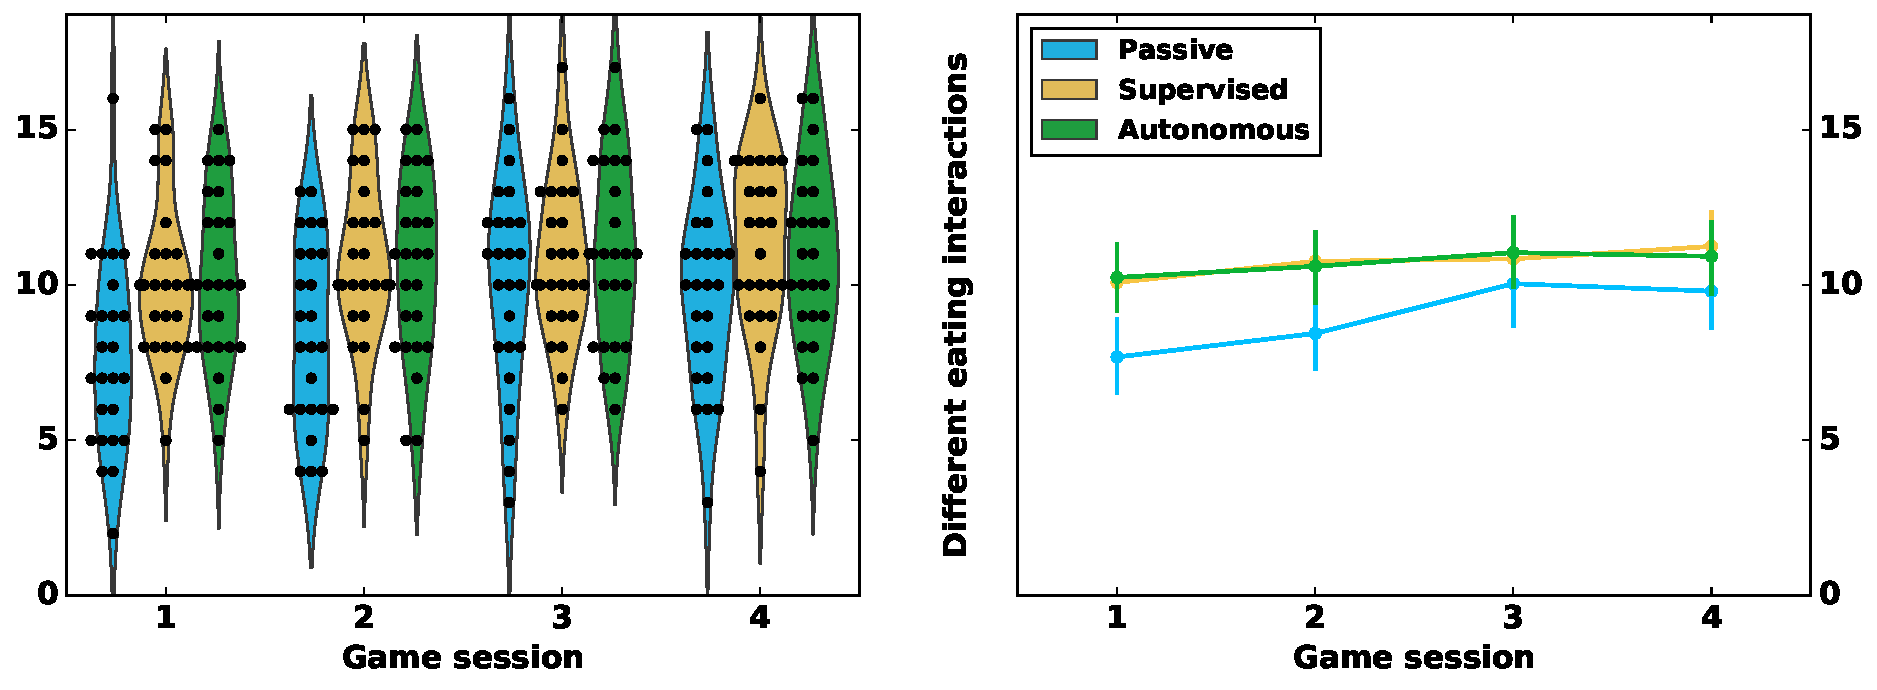
\includegraphics[width=1\linewidth]{d_eat.pdf}
	\centering
	\caption{Number of different eating behaviour for the four games for the three conditions.}
	\label{fig:tutoring_d_eat}
\end{figure}

\paragraph{Points}

Figure~\ref{fig:tutoring_points} shows the evolution of the number of points achieved by the children across the four game sessions. A Bayesian mixed-ANOVA showed an impact of the condition on the number of points achieved by the children in the game ($B=10.2$). Post-hoc tests showed a strong difference between the passive and the supervised conditions ($B=5.1$x$10^4$) and differences between the supervised and the autonomous conditions ($B=5.2$) and the autonomous and the passive condition ($B=5.9$). This indicates that when the robot was supervised, it allowed children to achieve more points than a  passive robot. And a similar effect was observed when the robot is autonomous, however the autonomous robot did not manage to reach the same efficiency as the supervised robot in helping the children to achieve a high score in the game.

\begin{figure}[ht]
	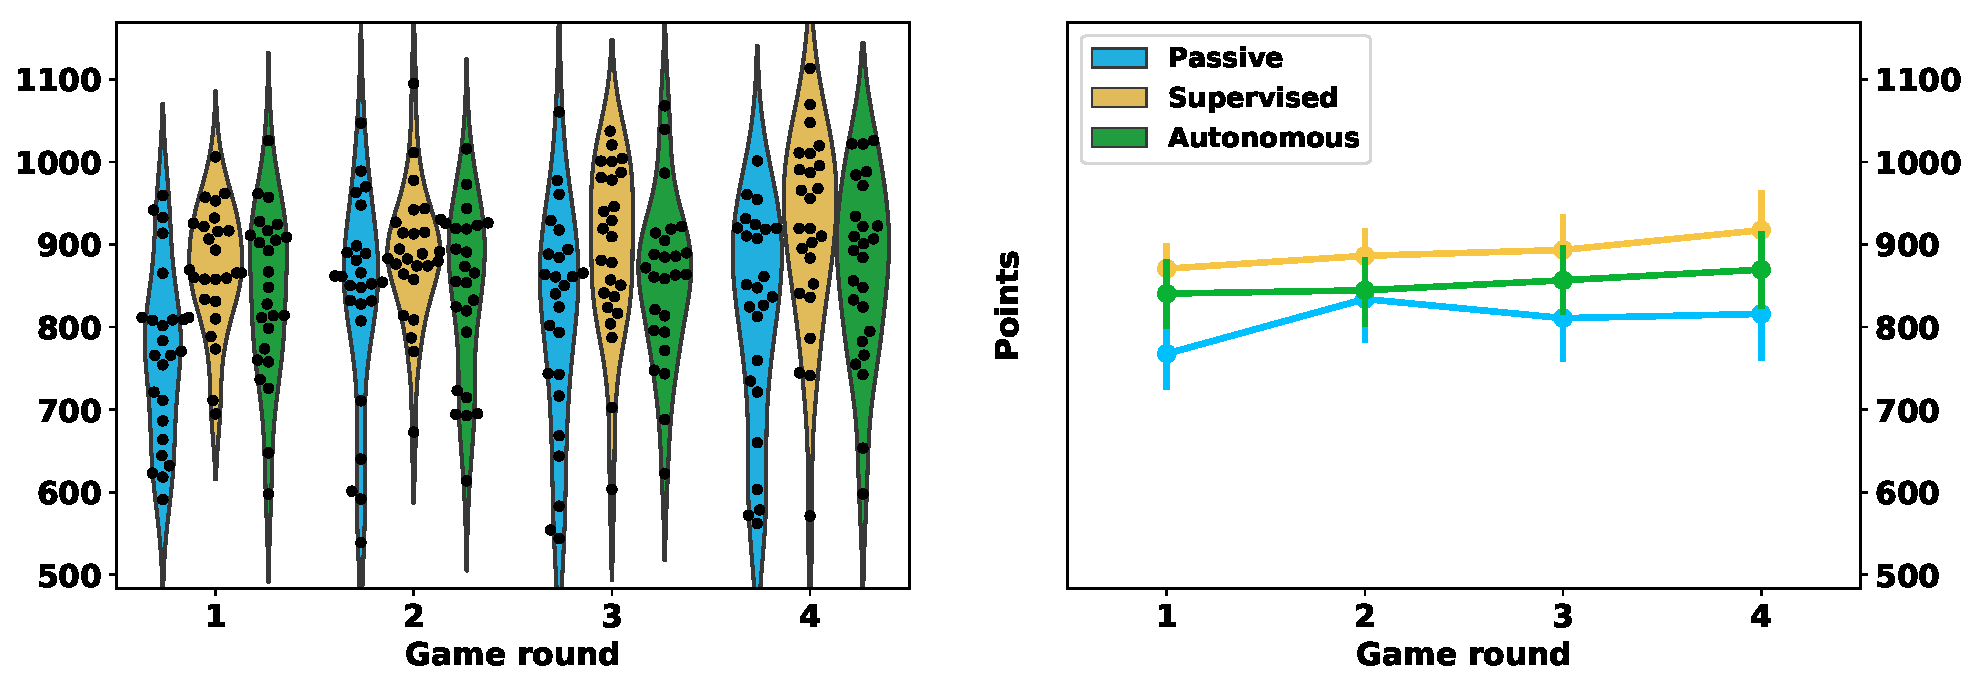
\includegraphics[width=1\linewidth]{points.pdf}
	\centering
	\caption{Points achieved by the children in each game session for the three conditions.}
	\label{fig:tutoring_points}
\end{figure}

\paragraph{Time}

Figure~\ref{fig:tutoring_time} shows the evolution of interaction time across the four game sessions. A Bayesian mixed-ANOVA showed inconclusive results on the impact of the condition on the interaction time in the game ($B=1.1$). However, post-hoc tests showed the absence of difference between the supervised and the autonomous conditions ($B=0.287$), whilst differences are observed between the supervised and the passive condition ($B=118$) and a tendency of difference between the autonomous and the passive conditions ($B=2.9$). This indicates that the supervised robot allowed children to be better at the game, allowing them to maintain animal alive longer than a passive robot. And the autonomous robot learned and applied a policy tending to replicate this effect and without exhibiting differences with the supervised one.

\begin{figure}[ht]
	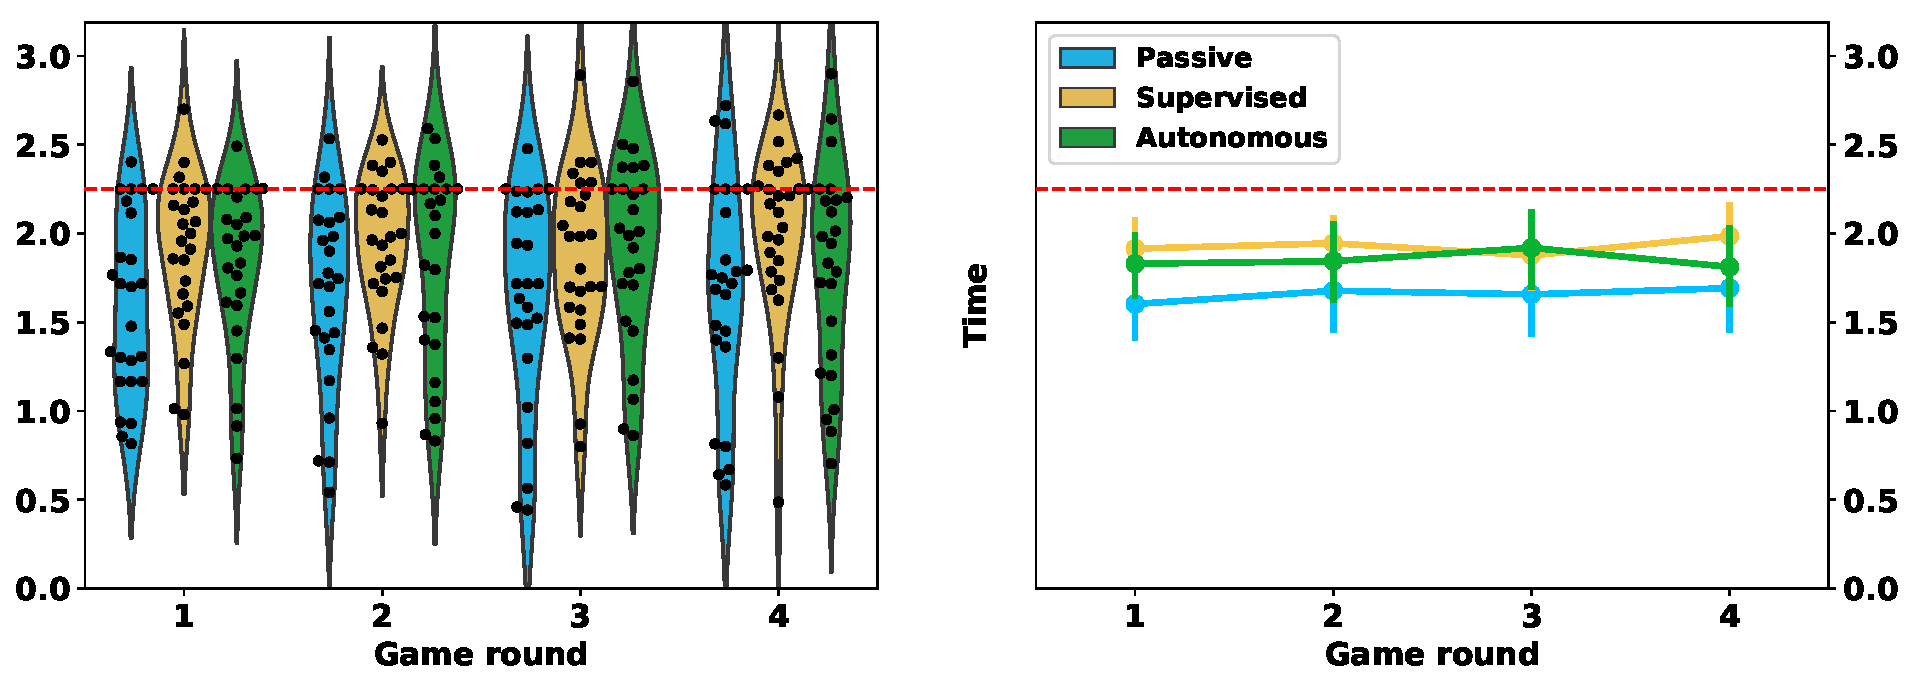
\includegraphics[width=1\linewidth]{time.pdf}
	\centering
	\caption{Interaction time for the four games for the three conditions.}
	\label{fig:tutoring_time}
\end{figure}


\paragraph{Summary}

These game metrics showed that the action policy executed by the autonomous robot allowed children to achieve similar results in the game than when the robot was supervised, and better results than when interacting with a passive robot. This provides support for H1 ("The autonomous robot is able to interact socially and efficiently during the game sessions and maintain the child's engagement during the learning task"). 
%However, children learned similarly in the three conditions, so these improvements in the game did not transfer to improvements in the test neither for the supervised robot nor the Autonomous one. This does not support H1 ("The robot support child learning: learning gain in passive condition $<$ learning gain in autonomous condition $<$ learning gain in supervised condition")

\subsection{Teaching the Robot}
Figure~\ref{fig:tutoring_supervision} presents the reaction of the teacher to the robot's suggestions across all the supervised sessions. In average the teacher accepted 22.3\% of all the proposition of the robot, which represented 35\% of all the actions executed by the robot and this effect tended to be stable across the sessions.

In post-hoc discussion, the teacher reported three phases in her teaching: 
\begin{itemize}
	\item First sessions: she was not paying much attention to the suggestions, mostly trying to have the robot executing a correct action policy.
	\item Session 6 to around 16: she was paying more attention to the suggestions without giving them much credit.
	\item Last sessions: she started to trust the robot more but without ever trusting it totally.
\end{itemize}

\ES{I should add more about it...}

\begin{figure}[ht]
	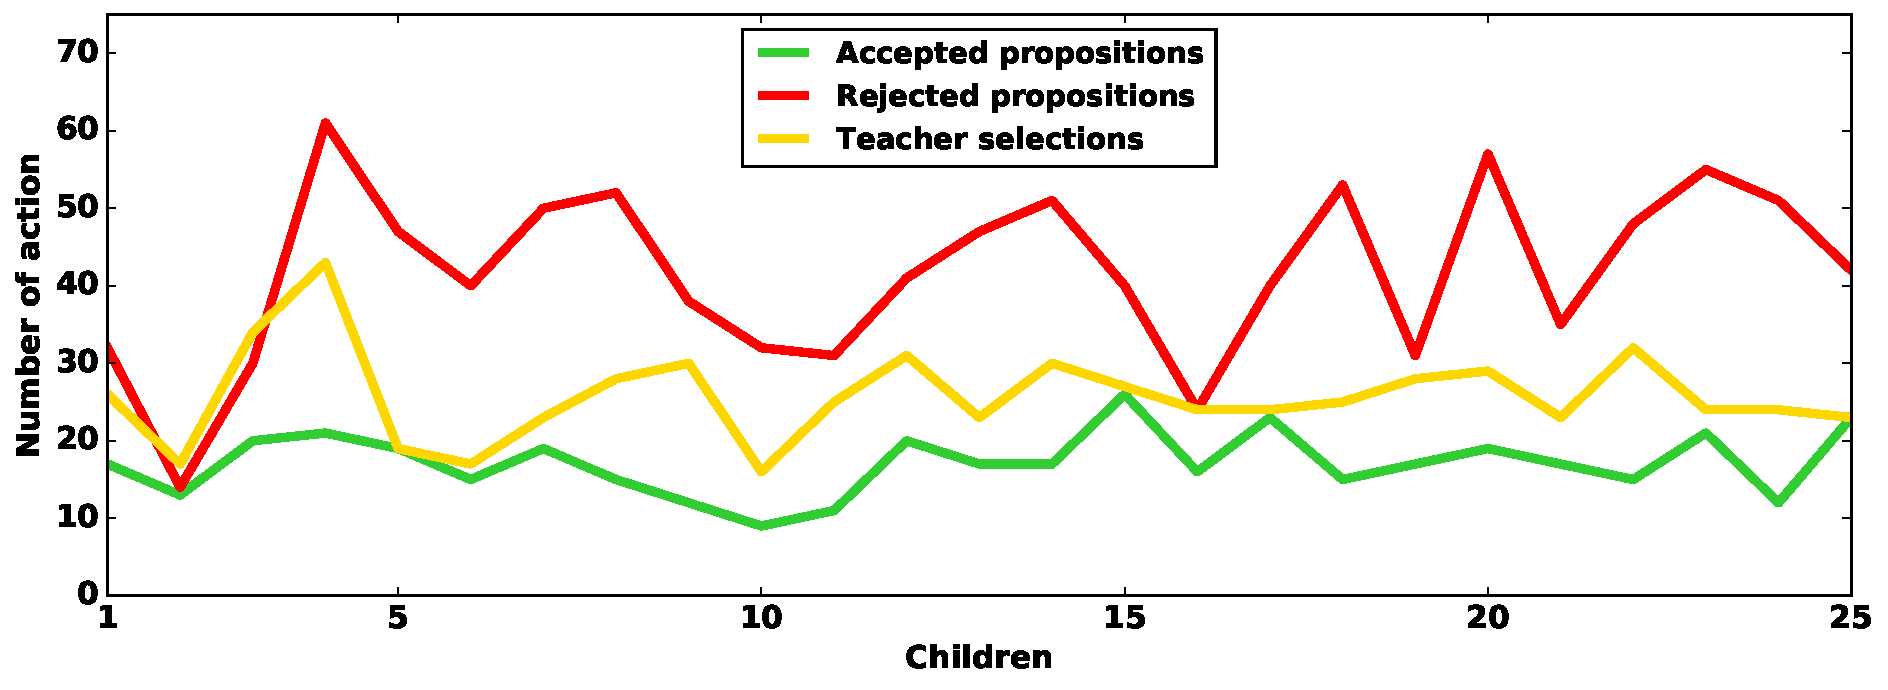
\includegraphics[width=1\linewidth]{./summary_supervision.pdf}
	\centering
	\caption{Summary of actions selection in the supervised condition: the `teacher selection' label represents each time the teacher manually selected an action for the robot to execute.}
	\label{fig:tutoring_supervision}
\end{figure}

The teacher did report a decrease of workload as she supervised the robot in more session. This was supported by behaviours such as typing her observations on a laptop, while gazing at the interface in multiple interactions (especially at the start of a session). However this decrease of workload seemed to be due mostly due to the teacher getting used to the interaction, and not to the online learning and the improvement of the suggested proposition, invalidating H3.
%Figure~\ref{fig:tutoring_proposition} presents the reaction of the teacher to the robot's suggestions across all the supervised sessions. In average the teacher accepted 22.3\% of all the proposition of the robot (by enforcing the action, let it be executed or using the `Do it' button), which represents 35\% of the actions executed by the robot. This effect tends to be stable across the sessions. The teacher interaction pattern evolved overtime, such as by using mostly the `Cancel' button in the start then the `Skip' one, but in the end, the teacher used this two buttons mostly interchangeably even if the algorithm underlying reaction is different. Another observation is the evolution from using the auto-execution function to the `Do it' button once the teacher felt more comfortable in the supervision. The teacher reported three phases in her teaching: 
%
%\begin{itemize}
%	\item First sessions: she was not paying much attention to the suggestions, mostly trying to have the robot executing a correct action policy.
%	\item Session 20 to around 65: she was paying more attention to the suggestions without giving them much credit.
%	\item Last sessions: she started to trust the robot more but without ever trusting it totally.
%\end{itemize}
%
%\begin{figure}[ht]
%	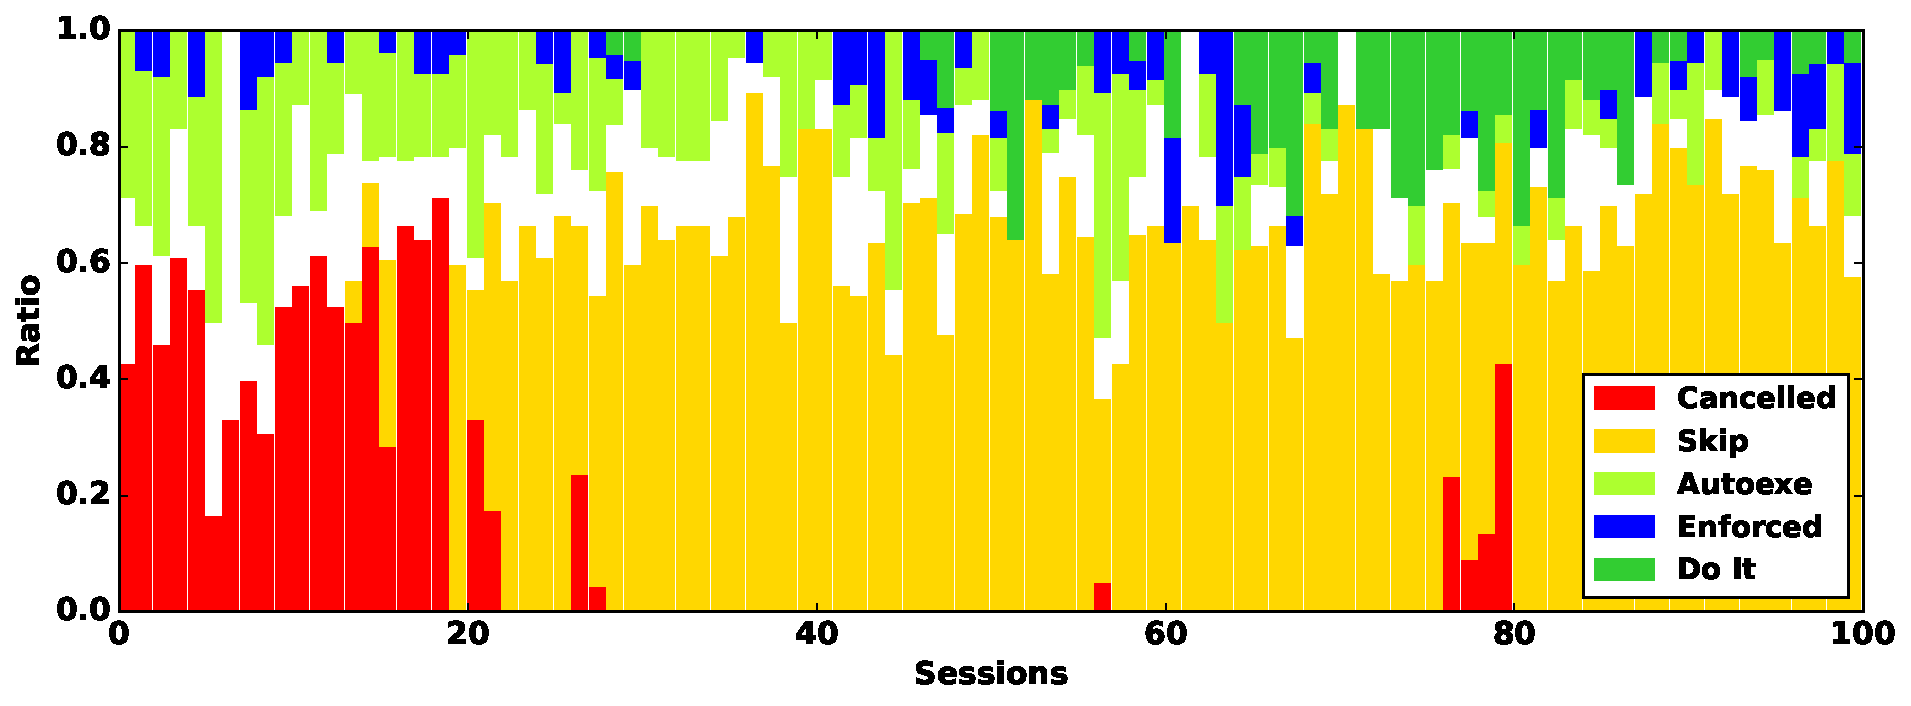
\includegraphics[width=1\linewidth]{propositions.pdf}
%	\centering
%	\caption{Teacher's reaction to the robot's propositions along the sessions.}
%	\label{fig:tutoring_proposition}
%\end{figure}
%
%
%\begin{figure}[ht]
%	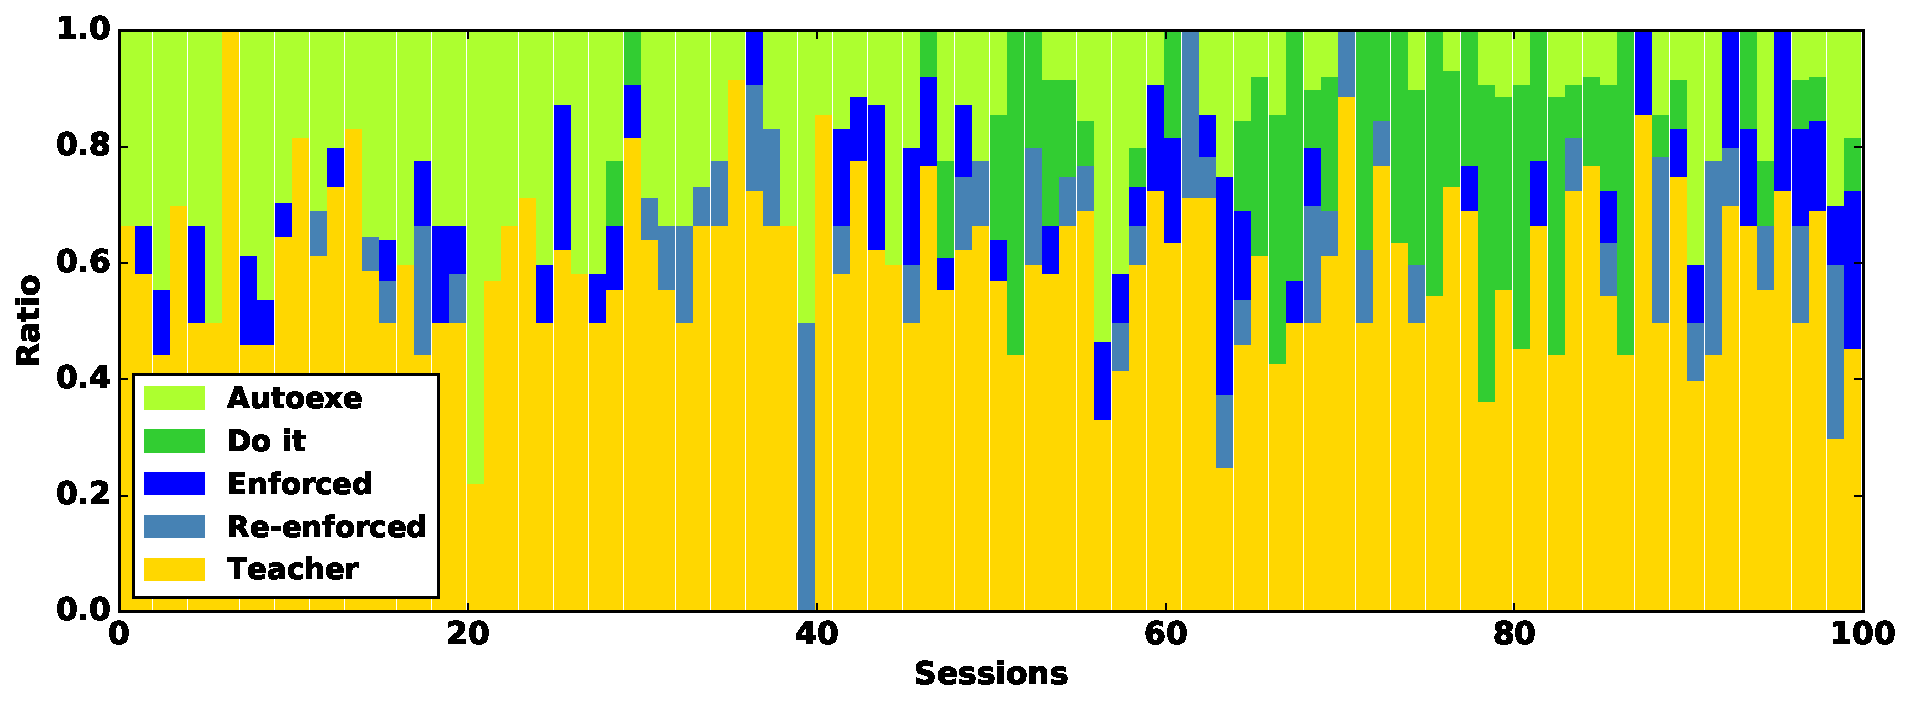
\includegraphics[width=1\linewidth]{selections.pdf}
%	\centering
%	\caption{Origin of the actions executed by the robot. Re-enforced actions indicates that an action has been selected after having been cancelled or skipped by the teacher.}
%	\label{fig:tutoring_selection}
%\end{figure}
%
%Additional comments:
%\begin{itemize}
%	\item The robot proposed in average 58\% more actions than the number of actions selected by the teacher.
%	\item As the time is continue and not discrete, the concept of correct actions is shifted, and actions selected by the teacher might have been proposed by the robot a fraction of second later without being counted as good proposition.
%	\item The teacher often cancelled/skip actions directly as they arrived without taking time to analyse them (limitation of this implementation of SPARC).
%	\item Evolution of teaching policy limits the potential of learning (not one single policy applied by the teacher, but an evolving one).
%	\item Children are different, so the teacher tried to apply different action policy for each child.
%\end{itemize}
%
%
%\begin{figure}[ht]
%	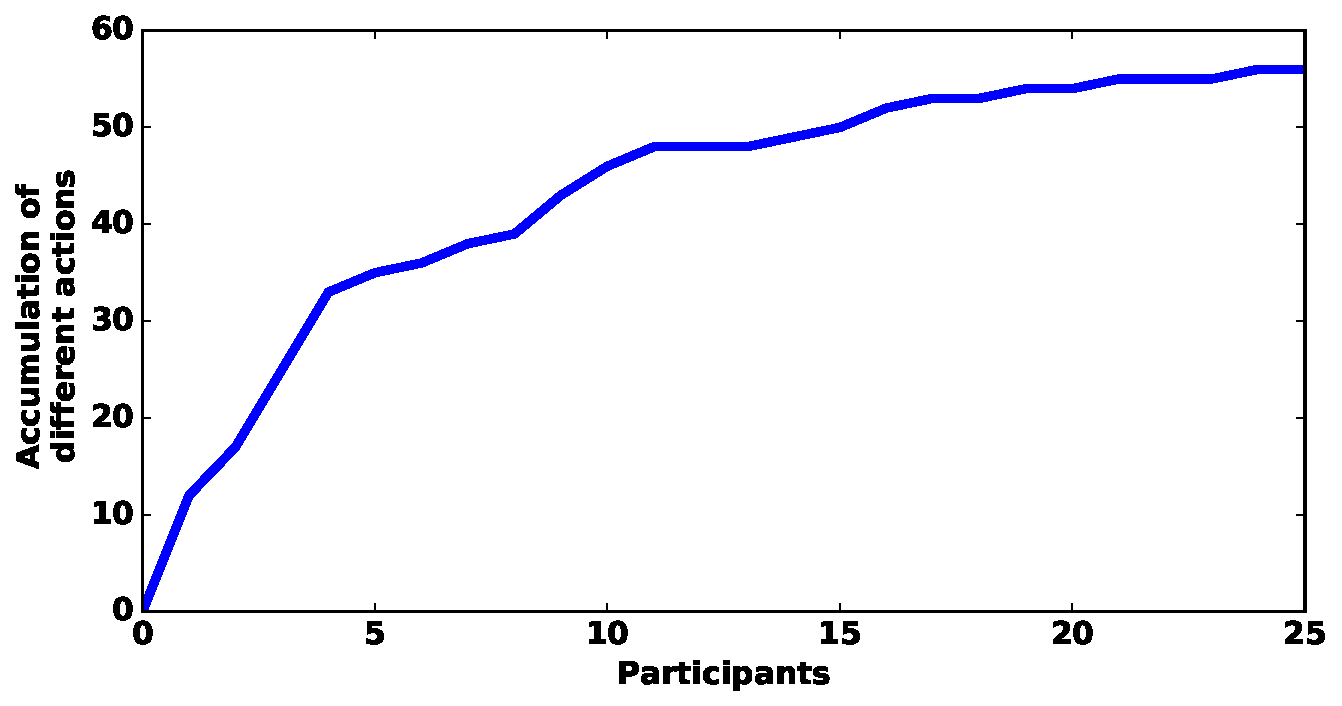
\includegraphics[width=.6\linewidth]{number_actions.pdf}
%	\centering
%	\caption{Accumulation of the number of different actions used by the teacher across the  participants.}
%	\label{fig:tutoring_actions}
%\end{figure}


\section{Discussion} \label{sec:tutoring_discussion}

\subsection{Children Behaviours and Learning Gain}

The active robot's behaviours encouraged children to produce more `useful' behaviours during the interaction. When interacting with the active robots, children encountered more situations with learning potential (such as the different eating behaviours). However, this additional exposure to learning items did not transform into an increase in learning gain. In the three conditions, the children learned similarly; thereby not supporting H2. We identified two possible roots for this absence of transfer between positive game behaviours and performance in the test. The first one is that the game by itself, without the robot, encouraged the children to explore and was sufficient to create learning. Children could learn solely from interacting with the game; consequently, the robot behaviour might have distracted children from their exploration. In that case two effects might have cancelled each other: on one hand the robot's behaviour provided additional knowledge to the child, but on the other hand the active robot perturbed their exploration of the game. This might explain the absence of effect of the robot's behaviour on the children's performance. The second possible origin would be in the test itself. The test only asked children to connect as many animals as possible, but children might have stopped connecting before showing all their knowledge. Accordingly, this way of testing children might not encourage them to demonstrate their exact knowledge. Having forced choices questions, for instance selecting randomly 20 connections and ask children if they are valid, might have provided a clearer evaluation of the children's knowledge. \ES{could be clearer}

%By only asking children to connect the animals they know, we do not force them to make a choice. They have the opportunity to stop the test at any time. This might limit the efficiency of the comparison as some children might continue further than other, and we might miss some knowledge about the children. It might have been better to select randomly 20 connections between the animals and ask the children if one animal can eat the other.

%\begin{itemize}
%	\item Game self-exploratory, robot behaviour might distract the children
%	\item no correlation between exposure to learning items and learning gains
%	\item Limits of the knowledge test: too open-ended, might have been better to have 10 random animals selected and ask the child to say yes/no?
%	\item Limit of the performance calculation: the test was probably not able to capture the exact knowledge of children - Learning is about discovering interactions
%\end{itemize}

\subsection{Robot Learning}
\ES{reorganise a bit}
One of the motivation of \gls{sparc} is that it provides a way to smoothly move a way from \gls{woz} to \gls{sa} and potentially pure autonomy. By learning online the action policy, the number of actions selected or corrected by the teacher would decrease and the number of accepted suggestion would increase, hence reducing the teacher's workload. However, this expectation (and by extend H3) was not validated by this study's observations. The number of action accepted, refused and selected by the teacher stayed roughly identical throughout the interactions. One of the reasons identified was that the robot proposed a large number of actions (58\% more than the total number of executed action). This indicates that the adaptive threshold restricting actions to be proposed was constantly too high. This high number of proposed actions partially explains the high number of actions refused by the teacher. As the robot tended to propose actions too often, the teacher reached a point in her supervision where she almost constantly refused the robot's propositions even in cases when they were correct. Another effect limiting the correctness of the proposition is the evolution of the teacher's policy. As the teacher progressed in the interactions, she increased the complexity of her action policy, adapting it to each child and using more and more different actions. As the algorithm could not predict actions not selected yet by the teacher, this lead to a requirement on the teacher to select new actions. Having such a moving target to learn probably limited the maximal performance achievable by the algorithm. Toward the last interactions, the number of different actions used by teacher tended to converge, this indicates that the algorithm might have achieved better results in the following interactions.

This study also stood out from classic problems using \gls{ml} on another point. In this study, the agent (the robot) interacted in a continuous time, whereas generally agents in \gls{ml} only exist in a discrete time. In discrete time, generally, an action has to be selected at each step, actions last one step, and optimal strategies can exist. However, when interaction in real time, actions take many steps and in most of the steps no action should be selected. Additionally, due to the continuous side of the time, actions are not valid at a specific step, but around that step. This imply that to reduce the teacher's number of selected actions, the algorithm does not have to select the same action as the teacher at each step, but needs to anticipate the teacher's actions, so that the teacher does not select them first. Such a requirement for the algorithm limits the visibility of results. The algorithm might a select correct action around the time the teacher would select it, but if that proposition arrived a step after the teacher's selection, it would not be considered as a good proposition.

An other element potentially explaining the limited efficiency of the online learning is related to the algorithm. In its simplest form, nearest-neighbours considers only one neighbour, making it highly sensitive to outliers \ES{cite}. Consequently, some instances in memory could be used too often, leading to an imbalance of policy (as observed when comparing the autonomous and supervised policy). One of the way to tackle this issue could be to the k nearest neighbours rather than only the closest one, this might have led to a more robust learning algorithm but this was not done in this study.

\ES{limit of use of feature selection in the study}

\ES{with more training data, and an algorithm addressing the fixable issues, the autonomous policy and the supervised ones should become closer and the workload on the teacher might decrease as the robot learns}

In such complex tasks, humans are making use of a large number of undefined \ES{ASK MADDIE} `states', especially temporal relations to select actions, and if the state definition the robot uses does not contains or cannot deal with these features, the learning will be limited.

 While the autonomous behaviour was different from the taught one, both policies still presented many similarities in the distribution of actions executed by the robot and the children's reaction to the behaviours. More training data and a better learning algorithm should even smoothen this difference of behaviour between the supervised and the autonomous robot and should also improve the learning process.

\subsection{Importance of the Teacher}

\gls{sparc} includes two distinct but simultaneous human-robot interactions. Thus, evaluating such interconnected interactions is a complex task: each human's behaviours will impact the other one. To explore a in a repeatable and comparable manner an interaction, the other one needs to be as constant as possible. However, humans are not constant and consequently evaluating these two interaction simultaneously is a challenge. By deciding to keep the same teacher for all the interactions, we only have a sample of one participant as a robot teacher. This could create some biases in the supervision, but as the teacher was not aware of the learning mechanism used for the robot and was not provided feedback on how to interact with the robot, these biases were limited. But, in essence, this study is a case study of one participant teaching a robot. It would have been interesting to try distinct teachers and observe how their different behaviours would impact the learning process and the final policy. We would expect that the resulting autonomous behaviours should match the multiple teachers' policy. However due to the number of children required to train and test the robot, we could not explore this axis. 
%
%\begin{itemize}
%	\item evolve their action policy
%	\item we had to fix her, so another teacher would have behaved differently
%\end{itemize}


%\begin{itemize}
%	\item The robot proposed in average 58\% more actions than the number of actions executed by the robot (approved and selected by the teacher): the threshold to select actions was probably too low, leading to too many propositions and the adaptivity of the threshold not good enough
%	\item As the time is continuous and not discrete, the concept of correct actions is biased, there is no `correct' action policy associating an action to each time steps. Additionally the timing of the proposition was key as actions proposed just after a selection would have been discarded.
%	\item To reduce the number of teacher selection, the robot would need to \emph{anticipate} every single teacher's action: not only knowing what action to do, but suggesting it the teacher before she started executing the action.
%	\item The teacher often cancelled/skip actions directly as they arrived without taking time to analyse them (limitation of this implementation of SPARC).
%	\item Evolution of teaching policy limits the potential of learning (not one single policy applied by the teacher, but an evolving one, including more actions as the teacher is more comfortable with the system).
%\end{itemize}

\subsection{HRI are Human Centred}

When a robot is supervised to interact with a human, and especially with a child, the main goal of the teacher is to ensure the experience for the child is optimal. Consequently, the teacher will be more focused on the child's behaviour than the robot learning. For instance, if an action would help the child but hinder the learning for a reason (for example an unusual child behaviour), the teacher will `damage' the robot learning to improve the child experience. In \gls{hri}, teaching the robot will always be only a side activity or a by-product of the interaction. 

Furthermore, in \gls{hri} the robot partners will be different persons, and as the teacher will adapt their policy to the specific person involved in the interaction, the resulting human policy will not one homogeneous policy applied to all the partners but potentially to one per person. This is a challenge for \gls{ml} as it increases the complexity of the task. The algorithm either have to learn a much larger action policy (covering all the different types of human partners) or learn a multitude of policies and be able to switch between them. Additionally, some of the feature used by the teacher to decide which type of policy to apply might not be available to the algorithm (for instance temporality or verbal utterance in our case). This implies that the algorithm might receive different demonstrations (outputs to match) for the same inputs, complexifying further the learning process.

%\begin{itemize}
%	\item Children are different, so the teacher tried to apply different action policy for each child.
%	\item Human centred interaction, the teacher was more focused on applying the best action policy for the child rather than teaching the robot.
%	\item Application will always be human-centered, so the teaching of the robot will always be a side activity: actions that can hinder the robot learning will be taken if the child would profit for them.
%	\item task complex
%\end{itemize}

\subsection{Opportunities} \label{sec:tutoring_opportunities}
\ES{careful with overlap between this discussion and the final one}

Despite the limitations of this implementation of \gls{sparc}, this study demonstrated the first application of \gls{sparc} to real \gls{hri}. A robot learned to interact efficiently with humans from in-situ supervision. \ES{Would that be the first time?} The autonomous robot produced an action policy similar to the one demonstrated by the teacher in the supervision, and the effect on the children were similar too (improvement of game metrics compared to a passive robot). This supports H1: the autonomous robot was able to interact socially with children and sustained engagement during the task (as demonstrated by the higher number of points and interaction time compared to the passive condition). This is an important contribution as the robot learned to interact in a complex task in the real world, including large state and action spaces and where errors could have an important cost on the interaction, potentially leading to a child refusing to continue the interaction.

Furthermore, this achievement also used a teacher without knowledge in robotics or \gls{ml}. This encourages the use of \gls{sparc} by a large part of the population and by extend increase the potential for people to be able to teach robots complex behaviours. This might help to reduce the entry bar of interaction with robots. If people do not need to know robotics or how to code to teach a robot a social behaviour, it may help to democratise the use of robots. While not have been explicitly demonstrated in this study, \gls{sparc} can also teach different behaviours using the same algorithm and state representation. Different teachers would teach the robots in dissimilar ways, therefore, the resulting autonomous behaviour would be adapted to each situation and would represent the teacher's policy. \gls{sparc} can be a way to allow non-experts in robotics to personalise their robot, to have it learn to behave in the way they each desire.

Even if the online learning did not reduce the teacher workload much through the interactions, \gls{sparc} possess two advantages compared to offline learning from \gls{woz} data using \gls{lfd}~\citep{sequeira2016discovering,liu2014train}. Firstly, the learning algorithm has access to more datapoints: the teacher's selection but also their reaction to the algorithm propositions. Secondly, by receiving feedback about the algorithm's knowledge, the teacher can create a mental model of the robot and have an idea of how accurate its action policy is. Furthermore, by interacting with the learning algorithm, the teacher can start building a trust grounded by their experience with the learner, potentially knowing its strengths and weaknesses. And this teacher's knowledge of the learner states can ease the decision of deploying the robot to interact autonomously as the teacher experienced the policy and knows what to expect from the algorithm.

%\begin{itemize}
%	\item Complexity of the task
%	\item discuss the supervision: not expert in machine learning, limited training
%	\item potential to extend robot teaching to a larger part of the population
%	\item potential to allow a same robot with the same algorithm to develop an action policy specific to its teacher: people can personalise their robot by teaching it how they desire it interacts
%	\item Way to support that the autonomous robot was also able to sustain the engagement through the learning task
%	\item Difference from offline learning from WoZ: possibility to gather more datapoints: teacher's selections and reactions to the robot's proposition => more points for learning
%\end{itemize}

%\subsection{Future work}
%\ES{probably irrelevant for this chapter}

%The work presented in this chapter could be extended and improve in a number of ways. First all the issues identified in Section~\ref{sec:tutoring_discussion} could be addressed, by using a more aggressive threshold, another way to test children's knowledge or using multiple neighbours to estimate the expected reward of an action. \ES{could extend} The learning game could also be modified to cover other teaching activities including moving images (potential application to language, maths).


%\begin{itemize}
%	\item Potential for other applications?
%	\item Ways to improve the study / How could the results have been better
%\end{itemize}
\section{Summary}

To conclude, this study proposed a new task for robot tutoring: a learning game to teach children about food webs, and most children involved in the study learned and improved their knowledge through the interaction. Additionally, for the first time in this research \gls{sparc} has been applied to teach a robot to interact with humans. By using a novel algorithm adapted from the nearest-neighbours designed to learning quickly in multidimensional states, the robot learned to produce a behaviour similar to the teacher's one. Furthermore, this teaching was performed by a user not expert in \gls{ml} or robotics. While not leading to improvements in the children's learning gain, the behaviours from both the autonomous robot and the supervised one did improve the performance of the children in the game. 

In summary, by this study we provided partial support for the main thesis of this research: ``A robot can learn to interact meaningfully with humans in an efficient and safe way by receiving supervision from a human teacher in control of the robot's behaviour.'' And, while presenting limits in the current versions (for instance by not reducing the teacher's workload over time), \gls{sparc} succeeded in its goal to allow a user non-expert in computer science to safely teach a robot to interact with humans. 
\cleartooddpage

%%%%%%%%%%%%%%%%%%%%%%%%%%%%%%%%%%%%%%%%%%%%%%%%%%%%%%%%%%%%%%%%%%%%%%%%%%%%%%
\chapter{Discussion} \label{chap:discussion}
\glsresetall

Chapter~\ref{chap:background} put the light on the absence of robot controllers today providing adaptivity to a robot with a low workload from humans and while ensuring that the robot's behaviour is constantly appropriate. Based on this observation, Chapter~\ref{chap:sparc} presented the \gls{sparc}, an interactive teaching framework designed to allow robots to learn a social interactive behaviour by being supervised by humans. Then Chapters~\ref{chap:woz},~\ref{chap:control} and~\ref{chap:tutoring} evaluated this approach in three studies, the last of which evaluated \gls{sparc} in real \gls{hri} consisting of a learning activity involving 75 children. Combined together, these chapters sought support for the thesis of this research:

\begin{quote}
	A robot can learn to interact meaningfully with humans in an efficient and safe way by receiving supervision from a human teacher in control of the robot's behaviour.
\end{quote}

Chapter~\ref{chap:woz} presented a first a study comparing \gls{woz} and \gls{sparc}. Results from this study demonstrated that a learning robot could reduce the human workload required to have it interact in the world without impacting its performance in the application interaction. This provide support for \gls{sparc} as a method allowing a robot to become progressively autonomous. 

The second study presented in Chapter~\ref{chap:control} explored how the control provided to the teacher by \gls{sparc} impacted the teaching of an efficient action policy. This study showed that by giving the human teacher control over the robot's actions, \gls{sparc} could ensure that the executed robot behaviour fits the teacher desires which led to a faster, safer and easier teaching. 

As the first and second studies were focused on the relation between the teacher and the robot, they had to use a repeatable and controlled environment to study \gls{sparc}. In contrast, the last study applied \gls{sparc} to a real-world \gls{hri}: child tutoring. In that study, an adult had to teach a robot to tutor children in an educational game. Results demonstrated that after having been taught using \gls{sparc} in multidimensional and generic state and action spaces, an autonomous robot displayed an efficient social action policy suited to interacting with children. The policies from the supervised and the autonomous robots presented similarities, and both policies resulted in more positive children behaviours compared to a passive robot. Whilst not reducing the workload on the human during the teaching process, \gls{sparc} demonstrated its applicability to complex, multimodal and high-stakes environment. During the teaching process, the teacher could ensure a useful robot action policy, which was maintained even after the teacher exited the control loop.

This chapter combines the results from the different studies presented in this research to discuss the findings. It starts presenting by how the three studies executed in this research work answered the research questions raised in Chapter~\ref{chap:intro}. Then, Section~\ref{sec:disc_limitations} presents the limitations of the approach proposed in this work, \gls{sparc}. Section~\ref{sec:disc_impact} discusses the more general impacts this research may have and the ethical questions raised by teaching robots to interact with humans.
%ethical questions raised when humans teach robots to interact with humans will be discussed in Section~\ref{sec:disc_ethics}, and Section~\ref{sec:disc_impact} will presents the potential impacts of this research. 
Finally, the last section proposes axes where \gls{sparc} could be extended to increase our knowledge in how humans teach robots, and improve \gls{sparc}'s usability and application to \gls{hri} and other fields.

%%%%%%%%%%%%%%%%%%%%%%%%%%%%%%%%%%%%%%%%%%%%%%%%%%%%%%%%%%%%%%%%%%%%%%%%%%%%%%
\section{Research Questions} \label{sec:disc_rq}

This section will revisit the research questions identified in Section~\ref{sec:intro_thesis} and explain how the work presented in this thesis addressed them.
\begin{itemize}
	\item [RQ1] \textbf{What are the requirements of a robot controller to ensure a behaviour suited to \gls{hri}?} 
	Based on a review of the different fields of application of social \gls{hri}, we defined three requirements a robot controller should follow to ensure an efficient interaction. First and foremost, the robot's behaviour needs to be constantly appropriate: as robots often interact with vulnerable populations, their behaviour needs to be constantly safe for the humans they interact with and helping the robot to achieve its role. Secondly, the robot should be adaptive, be able to generalise to unexpected situations, but also personalise its behaviour to the different humans it interacts with and be able to learn, improving and extending its action policy. Finally, the robot needs to be as autonomous as possible, or at least require a low human workload to interact in the world. This implies that robots needs to find ways to learn about their environment and reach autonomy without relying on random exploration as this would violate the first principle. We think the robotic community, and especially \gls{hri}, should strive toward more autonomous robots, and could take a stronger inspiration from \gls{iml} as it shows strong promises for teaching robots and could enable them to learn complex tasks such as interacting with humans.
	
	\item [RQ2] \textbf{What interaction framework would allow a human to teach a robot while validating the requirements from RQ1?}
	To validate the three principles expressed as answer to RQ1, we proposed \gls{sparc}, a new teaching framework for robots which provides control over the robot's actions to a teacher and use this control to learn in a safe way, validating the first and second requirements. Secondly, by allowing the teacher to passively accept the robot's propositions, we aim to decrease the workload on the teacher over time and progressively provide the robot with autonomy. By taking inspiration from \gls{iml}, \gls{sparc} aims to fill a void in the \gls{hri} research: online learning for interaction with humans.
	
	\item [RQ3] \textbf{Could a robot decrease its supervisor's workload by learning from their supervision?}
	Study 1 showed that providing a supervised robot with learning can reduce the workload on its supervisor. Furthermore, study 2 demonstrated that, compared to other methods, \gls{sparc} is an efficient way to enable a safe teaching and requires a comparatively low workload. Similarly to methods from \gls{lfd}~\citep{liu2014train,sequeira2016discovering}, \gls{sparc} provides an alternative to \gls{woz} and opens new opportunities to have robots displaying social behaviours after observing humans demonstrations. However, unlike classic \gls{lfd} methods, by including an online learning component, \gls{sparc} could produce results supporting the teacher during the learning process, inform them about the robot knowledge and potentially create trust between the robot and its teacher.
	
	\item [RQ4] \textbf{How does providing the teacher with control over the learner's actions impacts the teaching process?} 
	Results from study 1 and 2 indicated that by informing the teacher in advance of its actions, the robot ensures that its final behaviour is correct. This implies that even in early phases of the learning, when the robot behaviour is not adequate yet, the teacher can prevent the robot's lack of knowledge to negatively impact the world. Furthermore, this control helps the teacher to steer the robot toward useful parts of the environment and demonstrate it a good policy, making the teaching faster, safer, more efficient and lighter (as requiring a lower workload) than other methods lacking control. This finding is especially relevant to \gls{iml}, as often human teachers are provided limited control over the robot's action policy~\citep{thomaz2008teachable,knox2009interactively}. While being a challenge, providing the teacher with this control can have significant positive results on the learning progress.
\end{itemize}

Research questions 5 and 6 apply to the special case when \gls{sparc} is used to teach a robot to interact with a human. As such, the resulting interaction is as proposed in Figure~\ref{fig:concept}: a triadic interaction between a human-target, a robot and a human teacher.

\begin{itemize}
	\item [RQ5] \textbf{How does teaching a robot to interact socially impacts the two humans involved in the overall triadic interaction?}
	When being used to teach a robot to interact with a human, \gls{sparc} does allow the robot to constantly have an efficient behaviour (as demonstrated by the improvement of children's behaviours in the supervised condition in Chapter~\ref{chap:tutoring}). However, this performance in the application interaction might come with a cost for the teaching interaction. As the teacher needs to react to the robot's suggestions, they also have to monitor a second autonomous agent, which might lead to a heavier workload than classic teleoperation methods. This is one of the drawbacks of \gls{sparc} compared to methods based on \gls{lfd} to gather information, but as mentioned earlier, ways exist to mitigate this issue and allow this interaction between the teacher and the robot to lead to positive results for the teacher.
	
	\item [RQ6] \textbf{After receiving supervision from a human, could a robot behave autonomously in a social context?}
	In Chapter~\ref{chap:tutoring}, we used \gls{sparc} to teach the robot in the supervised condition, and then we deployed the robot to interact autonomously. During this autonomous interaction, the robot applied a policy similar to the demonstrated one, and the impact on the children's behaviour was close to the one in the supervised condition. Consequently, in this study, the robot managed to behave socially in an autonomous fashion in a complex and multimodal environment after having been supervised by a human in a learning phase. This finding is one of the most important of the thesis as it demonstrates the potential of \gls{sparc} to teach robot complex social autonomous behaviours.
\end{itemize}

\section{Limitations of SPARC} \label{sec:disc_limitations}

\gls{sparc}, as presented in Chapter~\ref{chap:sparc}, is a framework which has been used to teach robots to interact with humans or in high-stakes environments, but which presents several limitations restricting the range of domains it could be applied to.

\subsection{Requirement of a Human in the Loop}
%The first of these limitations is the requirement of a human to supervise the robot, even once it has learn an action policy. As stated earlier, \gls{sparc} aims to move away from \gls{woz} or other teleoperation methods by learning an efficient action policy from the human commands. 
%Classical methods to teach robot to interact with humans are based on \gls{lfd}: during a data acquisition phase, a human teleoperate the robot or interact  
%In its original framing, \gls{sparc} did not aim to create a fully autonomous agent behaving without supervision, but to progressively provide a robot with autonomy by smoothly decreasing the reliance on a human to control it. In that case, there is no interaction where the robot is fully autonomous, the human teacher is constantly in control of the robot's actions using \gls{sa}. This differs from \gls{lfd} methods which generally have a teacher manually controlling a robot in a first phase, while the robot is deployed to act autonomously in a second one. During this single phase, the workload on the supervisor would decrease as the robot learns while a high performance in the domain application would be maintained due to the control provided to the teacher. However, \gls{sa} still requires a human involved in the supervision and as such presents limited applicability to fields where robots are expected to fill gaps in human workforce or to reduce the requirements on humans. 

The first of these limitations is the requirement of a human to supervise the robot, even once it has learn an action policy. As stated earlier, \gls{sparc} aims to move away from \gls{woz} or other teleoperation methods by learning an efficient action policy from the human commands. In its original framing, \gls{sparc} did not aim to create a fully autonomous agent behaving without supervision, but to smooth the teaching phase and the use phase into one single interaction using \gls{sa}. In this single phase, the workload on the supervisor would decrease as the robot learns while a high performance in the domain application would be maintained due to the control provided to the teacher. However, \gls{sa} still requires a human involved in the supervision and as such presents limited applicability to fields where robots are expected to fill gaps in human workforce or to reduce the requirements on humans. 


Despite not being the original goal, \gls{sparc} can still be used to create a fully autonomous behaviour (as demonstrated in Chapter~\ref{chap:tutoring}). In that case, the training process would be similar to \gls{lfd}, with a training phase using \gls{sparc} and then the testing/deployment phase of the autonomous behaviour. However, by using \gls{sparc} differences remain. First, during the training phase, instead of passively receiving commands from the teacher, the robot would proactively make suggestions to the teacher. As presented in Section~\ref{sec:tutoring_opportunities} this aims to reduce the workload on the teacher during the training phase, provide more datapoints for the learning and inform the teacher about the state of robot's knowledge, potentially creating trust between the robot and its teacher. Second, even after being deployed to interact autonomously, the teacher could still step back in control using \gls{sparc} again to refine the action policy. Alternatively, if a different behaviour has to be applied (e.g. if the robots interact with a child with special needs rather than a typical one), the teacher can take over using \gls{sa} to ensure a personalised experience for this specific interaction.

\subsection{Reliance on Human's Attention}
%\ES{reread}
A second limitation of \gls{sparc} lies in the constant need for the human's attention and the presupposition that human teachers will always ensure an appropriate robot behaviour if given the opportunity. Throughout this research, we assumed that even if the robot behaviour may be mostly correct, the supervisor would be attentive to the robot suggestions and ready to correct any error at any time. This assumption is similar to autonomous cars using a safety driver or Tesla Autopilot requiring continuous human supervision. The agent is fully autonomous but may make mistakes and as such, a human needs to be ready to correct these errors before they impact the world. However, as demonstrated by the accidents in 2017 and early 2018 involving these supervised autonomous vehicles, this assumption is often violated, and a short moment of inattention may have dire consequence\footnote{Cf. the Tempe and Mountain view accident reported by the media in early 2018.\label{foot:disc_danger}}. By observing a seemingly correct agent behaviour for an extended period of time, the human supervisor might start to overtrust the agent, missing the occasion to react in time to anticipable errors potentially leading to frustration or death in the case of autonomous vehicles\footref{foot:disc_danger}. Nevertheless, some ways exist to mitigate this limitation but have not been applied to autonomous driving or general \gls{iml}. For example, with \gls{sa} the agent informs in advance the supervisor about its actions, similarly a car could display the planned trajectory on a screen or in augmented reality. This would provide the supervisor with more time to analyse the situation potentially allowing them to react in a timely fashion. Alternatively, the agent could communicate a lack of confidence in its actions or its interpretation of the environment, informing the supervisor that attention is specially required in that moment.

\subsection{Time Pressure}
%\ES{check}
As pointed already in Section~\ref{ssec:sparc_time}, with \gls{sparc}, the presence of the \gls{cw} and the auto-execution of actions may lead to issues. To be applicable and make use of the auto-execution of actions as a way to reduce workload, the \gls{vw} of an action needs to be wider than its \gls{cw}. That way, actions approved passively are still valid when executed. To increase the application of \gls{sparc} to a wider range of situations, the \gls{cw} has to be as narrow as possible. In contrast, the supervisor needs a \gls{cw} as wide as possible, to provide them with enough time to process the action and cancel it if required. Correction windows too narrow would put additional pressure on the supervisor to react in time or even prevent them to avert undesired actions. %To cope with this additional time pressure, the supervisor might find ways to prevent the suggestions of actions or simply refuse each action proposed by the robot. 
This results in two effects having opposite requirements on the \gls{cw}. However, while a longer \gls{cw} would only limits \gls{sparc}'s applicability in some situations, one too short could have negative consequences. As such, this need of a \gls{cw} wide enough to allow the teacher to react is probably on of the main limits of \gls{sparc} as it produces a significant delay in the robot's actions and reduces the range of domains \gls{sparc} can be applied to.

%\ES{reread}
However, this requirement of a \gls{cw} wide enough for the teacher can be mitigated in multiple ways. For example, instead of communicating the action the robot is directly about to do, the robot could communicate a plan with multiple steps announced in advances. That way, the teacher would be informed beforehand of the next few steps and could anticipate their impact and react to any future actions instead of limiting their evaluation to the next one. Alternatively, the robot could adapt the length of the \gls{cw} to its confidence in the proposed action; for instance, an action with a low confidence would be given more time to be corrected. Likewise, each type of action could have a dedicated value for the \gls{cw}, for example actions needing to be executed quickly (such as emergency breaking for example) would have a much shorter \gls{cw} than other actions with less time constraints. Finally, a last possibility could be to allow the teacher to manually select the duration of this \gls{cw}, consequently letting them be in control of the pace of the interaction. In that case, the teacher might prefer to start with a long \gls{cw} and make a limited use of the auto-execution in the early phases of the interaction to be able to focus on the teaching process; but in later stage of the interaction, they might reduce this \gls{cw} to profit for the auto-execution of actions and reduce their workload.


\subsection{Overloading the Teacher}

By giving an active role to the robot in the teaching process (through proposing actions), \gls{sparc} requires from the teacher to  monitor simultaneously two autonomous agents: the human target and the robot. This requirement might lead to another risk with \gls{sparc}: overloading the teacher with suggested actions. If the teacher has to correct more actions than they would have selected, their workload would not be reduced but increased. While still providing useful information for the learning algorithm (and more than only the actions selected by the supervisor), this supplementary workload on the teacher is not desired. As explained in Chapter~\ref{chap:tutoring}, this could lead to erroneous teacher's behaviours hindering the learning and potentially increasing the risks in the interaction. For example at some points in the study presented in Chapter~\ref{chap:tutoring}, the teacher just cancelled actions as soon as they arrived, even before she had time to evaluate them. While reducing the workload on the teacher by not requiring them to evaluate the proposed action, this behaviour might limit the efficiency of the learning algorithm by giving it incorrectly labelled datapoints. 

Overloading the teacher is a serious issue and might have negative consequences both on the robot's learning and the experience of the human involved in the application interaction. As such, mechanisms must be present to ensure that this does not happen. The learning algorithm needs to have the right balance between suggestions and waiting periods to allow the teacher to analyse and provide a correct evaluation of the proposed actions. Alternatively, the teacher could be provided a direct way to impact on this suggestions and on the auto-execution of actions to give them control over their workload and allow them to teach the robot efficiently.

\subsection{Interface}\label{sec:disc_lim_interface}

The interface between the teacher and the robot is key when applying \gls{sparc} or other \gls{iml} methods. Simple interfaces can be easy to create and used by the teachers, however they might only have limited efficiency in the learning process. For instance, approaches using only feedback require a single one-way communication channel between the teacher and the robot, and this channel only needs to send a scalar evaluation of the agent's actions. Consequently, both the design of the interface for the teacher and the communication are simple but their efficiency is limited. On the other hand, to provide full control and accountability over the robot's actions, \gls{sparc} requires both ways communication. First, the teacher needs to receive inputs from the robot, such as its intentions, to decide if the action is valid or not. Second, the teacher needs to send information to the robot: feedback about the intentions, to preempt actions if required, but also demonstrations by selecting actions for the robot to execute. As the robot may have access to hundreds of actions, assigning one button per action is not feasible, other ways of commanding the robot need to be found. Furthermore, as mentioned in Chapter~\ref{chap:sparc}, with \gls{sparc} the teacher can also provide additional information to the algorithm to speed up the learning. In summary, the interface between the robot and the teacher needs to provide the teacher with the robot's intentions and allow the teacher to preempt actions, select any action and provide additional information to the learning algorithm. An interface providing all these features can easily be confusing and difficult to use by humans, increasing even more the required workload to control and teach the robot. As such, for applying \gls{sparc} to complex environments, efforts need to be invested in the interface to make it intuitive and clear. 

For instance, in Chapter~\ref{chap:tutoring}, the \gls{gui} used by the teacher represented the current state of the game, with some buttons for accessing a subpart of the action space, but the majority of actions was inferred by the way the teacher moved items on the screen and the items selected. An alternative way could be to use natural language. Humans are experts in using natural language to communicate and the open-endedness of this tool makes it suited for applications of \gls{sparc} where the teacher can speak and where the time required to vocalise commands is not critical, such as a robot assistant at home.

\subsection{Learning with Humans}

%As justified in Chapter~\ref{chap:background}, today, there is no simulator of humans and social norms precise enough to be used to train robot to interact with humans. Consequently, learning for \gls{hri} has to happen in the real world. In addition to this \emph{space} constraint, learning with humans also adds a \emph{time} constraint. B

\gls{sparc} has been designed to enable agents to learn safely \textit{in situ} for high-stakes environments where no simulator can be used to learn in a virtual world (e.g. \gls{hri}). However, learning \textit{in situ} for interaction with humans adds a serious time constraint: by including a human in the learning interaction, this interaction needs to go at a human pace. This implies that gathering datapoints through \gls{sparc} is a relatively slow process. 
Consequently, recent algorithms relying on large datasets (or ease to collect large amount of data)\footnote{For instance ImageNet contains more than 14 millions of images~\citep{russakovsky2015imagenet} and \gls{rl} methods still rely on millions or more of datapoints (cf. Section~\ref{ssec:back_rl})} have limited applicability for learning online to interact in the real world. 
%And recent progress in \gls{ai} being linked to the availability of large datasets or the ease to collect large amount of data, many recent algorithms are not applicable when learning online in the real world. 
As such, algorithms using \gls{sparc} need to be data efficient, be able to learn from a low number of datapoint and generalise quickly. However, as mentioned previously, by including the human in the loop and learning in the real world, we have access to important additional features. First, the points accumulated should be relevant to the learning process: they come from the desired interaction and as they have been validated by a human, their label should be correct. And secondly, the human can also provide additional information on the selection to quicken the learning (as implemented in Chapter~\ref{chap:tutoring}). This fuller use of the human teacher might help to mitigate the limited number of datapoints available when learning in the real world to interact with humans.

%\subsection{Experimental Limitations} \label{sec:disc_experiments} 
%\ES{Need to be sure that all these limitations are mentioned in the corresponding parts}
%Similarly to the method proposed in this research, the studies evaluating \gls{sparc} also presented some limitation. 

%The first study presented in Chapter~\ref{chap:woz} used participants familiar with robots. One could argue that this population is not representative of the general population expected to interact with robots. However, and as explained in that chapter, in many case in \gls{hri}, the wizards teleoperating robots are trained experts knowing the robot used in the interaction and how to control it. Thus, the participants involved in that study are representative of a significant part of the population expected to supervise a robot to interact with other humans. Additionally, the small sample of the study (N=10 for a within participants design) explains why no significance testing have been done in the study. However, valuable information have been collected and helped us to design the two other evaluation of \gls{sparc}. A last potential limitation of the evaluation relates to the discretisation of time. In this study, the \gls{woz} condition was not a real \gls{woz} as the participants needed to select an action (or accept a random action) at each step. However, this made the two conditions more comparable and the amount of workload on the supervisor in the \gls{woz} condition should have been similar to a real \gls{woz}.
%\ES{low number of datapoint and slower interaction}

%%%%%%%%%%%%%%%%%%%%%%%%%%%%%%%%%%%%%%%%%%%%%%%%%%%%%%%%%%%%%%%%%%%%%%%%%%%%%%
\section{Impact} \label{sec:disc_impact}

\subsection{Pushing the State of the Art}

Before the start of this research work or even during its realisation, few other methods have been applied to teach robot to interact with humans. As mentioned in Chapter~\ref{chap:background}, the main other approaches were \gls{lfw} and \gls{lfd}, they used demonstrations from a \gls{woz} setup or interactions between humans and from these demonstrations learned offline an action policy~\citep{knox2014learning,liu2014train,sequeira2016discovering}. Due to the challenges when learning during the interaction (high stakes of actions, limited datapoints and complexity to maintain a policy providing useful data), online learning and \gls{iml} were seldom used to teach robot to interact with humans, these approaches were mostly focused on teaching agents to interact in other non-social environments. Additionally, most of the previous methods in \gls{iml} only provided limited control to the human teachers, reducing them to feedback providers while humans could and should provide much more information to learning agents~\citep{amershi2014power}
	
By proposing \gls{sparc}, we wanted to push \gls{iml} to give more power to robot teacher, to make a better use of humans abilities to improve the learning process, making it safer and more comfortable for these human teachers. By keeping a human in control of the robot's actions, \gls{sparc} enables robots to learn online in sensitive environments. %, we pushed the state of the art to new boundaries in teaching robots. 
%With \gls{sparc} we proposed a new way to teach agents. By following the principles presented in Section~\ref{sec:sparc_principles} (combining \gls{sa} and \gls{ml}), this method provides a robot with an adaptive policy while ensuring that its behaviour remains constantly appropriate. 
Furthermore, with the combination of proposition, correction and selection of actions, \gls{sparc} has the opportunity to reduce the workload on the teacher. Hence, this approach is fit to control and teach robots to interact with humans as it follows the requirements presented in Section~\ref{ssec:back_constraints}. With this method, we successfully demonstrated in Chapter~\ref{chap:tutoring} that robots can be taught online to interact efficiently with humans, while ensuring a constantly appropriate action policy. By using a new algorithm and keeping the teacher in control, \gls{sparc} allowed a robot to learn a social and technical action policy in a high dimensional and multimodal sensitive environment.

By demonstrating its applicability to teach robots to interact with humans from \textit{in situ} supervision, \gls{sparc} pushes the state of the art both in \gls{hri} and \gls{iml}. By building on \gls{lfd}, \gls{sparc} keeps its advantages: allowing to teach behaviours complex to define or not known in advance. However, by including an online learning component and keeping the teacher in control, this new method might allow robots to be deployed in new contexts where they are absent today.

%\ES{presents goods and bads: advantages of both approaches, learning offline and online}
%; therefore, with \gls{sparc} the resulting autonomous behaviour can be adapted to each situation and represents the teacher's desired policy. %\gls{sparc} can be a way to allow non-experts in robotics to personalise their robot, to have it learn to behave in the way they each desire.

\subsection{Empowering Non-Experts in Robotics}

%\ES{other methods require a lot of engineering between the demonstrations and the applications, sparc smoothes the process, allowing the engineering work to happen before, hence allow people to teach their robot themselves}

Other methods used to teach robots to interact with humans use post processing on previously gathered demonstrations to learn offline an action policy. While leading to positive results, these approaches require significant engineering work after the demonstrations have been recorded to create a robot behaviour and provide limited opportunities to refine the behaviour after the learning is over~\citep{liu2014train,sequeira2016discovering}. This implies that they cannot be used solely by end-users not knowledgeable in machine learning, experts in robotics have to interpret the data provided by the domains expert to design the behaviour. In contrast, by mixing together the collection of data and the learning, \gls{sparc} removes this barrier between data collection and use. That way, end-users can directly teach themselves a robot to interact as they desire.
%By allowing end-users non-expert in robotics to teach a robot how to interact, 
\gls{sparc} provides an opportunity for anyone to personalise their robot without requiring technical skills. As demonstrated in Chapter~\ref{chap:woz} and~\ref{chap:control}, from a single algorithm and state representation, \gls{sparc} can lead to different behaviours adapted to the teacher's strategy and preferences. Combined with efficient interfaces and learning algorithms, approaches such as \gls{sparc} have the potential to democratise robotics by allowing anyone to teach a robot to interact efficiently in a wide range of domains. Robot developers and designers could use this learning ability to deploy robots as \emph{blank slates}, with just a way to perceive the world, act on it and interact with a teacher, and let their behaviour be defined by their users. These users would start filling these blank slates, creating their own robot behaviour, teaching their robot how to fulfil their personal needs. As defended by \cite{fails2003interactive} and \cite{amershi2014power}, by allowing end-users to teach an agent to behave as they desire, \gls{iml} methods have the potential to ease the deployments of technology and reach faster new application domains. This might allow users currently excluded from using robots (due to lack of interest from developers and lack of technical skills from the users), to profit from this new technology.

While providing many opportunities, deploying a blank robot able to learn complex action policies would require significant engineering pre-deployment to have a wide enough state and action space and a learning algorithm efficient enough to reach useful policies. However, as demonstrated by the study in Chapter~\ref{chap:tutoring}, this is achievable. A robot can be deployed with large state and action spaces and then using algorithms designed to learn quickly from teachers in complex environment, a non-technical human can teach a robot a complex social policy. Furthermore, by providing additional tools to the users to widen or refine the state and action space, this teaching could be applied to even more applications.

%As different teachers have various preferences, they will have different expectations for the robot's behaviour. And \gls{sparc} could be a way to allow each user to teach their robot a personalised interaction behaviour.


\subsection{Robots and Proactivity}
%\ES{bad}
Another way to interpret \gls{sparc} is as a way to provide proactivity to a robot. By using \gls{ml} and proposing to execute actions, the robot is actually taking the initiative to do an action without executing it straight-away. For instance, a proactive robot assistant would anticipate its user's needs and desires and would propose help or services without having to be asked~\citep{mason2011robot}. This capability has two uses: first it allows robot users not to have to ask a supportive behaviour from the robot every time they need it and second, it means that the robot could even support its user when they do not realise help would be useful.

By having the capability to learn new actions, or what action it should do, such a robot would move from a simple tool to use to an adaptive partner able to support its user in a large quantity of task. Finally by informing the surrounding humans of its actions, such a robot assistant would only execute action deemed useful by their users limiting the risks of negative outcomes.

\subsection{SPARC Beyond Human-Robot Interaction}\label{sec:disc_beyond}

Interactions with humans are complex: they require social behaviours in large multimodal environments, with high stakes and where gathering datapoints is a tedious process. As \gls{sparc} demonstrated its efficiency on such an environment, it should be possible to apply it to many other domains outside of \gls{hri} where constraints on the learning process are lighter. For example, it could be used to teach robot manipulation or navigation task: a simulator could present the expected trajectory leaving the teacher time to correct it if needed. Alternatively, and similarly to other \gls{iml} approaches~\citep{fails2003interactive}, \gls{sparc} could also be applied to classification tasks, maintaining the user informed about the state of the algorithm's knowledge and involving them in the learning process. For example, for semi-supervised image classification, the algorithm could automatically present to the user a subset of classified images between learning steps, and this user could step in when a misclassification happens. In these cases, where incorrect actions have limited impacts, the corrections can happen in hindsight, as proposed in \cite{chernova2009interactive}. Finally, the principles of \gls{sparc} could also be used to support agents using \gls{rl} in the real world. The supervisor could provide a safeguard preventing the agent to make errors, bringing it back to the correct parts of the environment or guiding the agent to the relevant actions in complex environments.

\subsection{Ethical Questions} \label{sec:disc_ethics}
%\ES{add more ref to support the questions}
Having robots interacting in human environment and allowing any human to teach them, raise multiple ethical questions~\citep{lin2014robot}.

The first one concerns people's jobs. Throughout robots and machines history, many jobs have been automated and more are expected to disappear in the next years~\citep{frey2017future}. And as \gls{sparc} allows non-experts in computing to teach robot, it might foster the deployment of robots in social environments, such as schools or care facilities. The arrival of robots in such sectors might lead teachers or social workers to fear for their jobs. However, in many of such social environments with no direct quantifiable return on investment, workforce is already lacking (e.g. nurses in the US; \citealt{nevidjon2001nursing}) and this shortage is expected to grow in the future. Consequently, robots provide an opportunity not to replace a workforce already in shortage of workers, but on the other hand to support these people in their job, making these jobs safer and more pleasant for the workers and providing additional support for the clients or patients~\citep{wada2005psychological}. However, the \gls{hri} community as a whole needs to be aware of these fears and ensure by their work that robots have a positive impact on society and communicate their vision of robots helping the human population.

As mentioned in the previous paragraph, by allowing anyone to teach a robot, \gls{sparc} might increase robots' range of application, potentially leading to more interactions with vulnerable populations, such as elderly people or children in school. However, having robots interacting in these environments raises multiple questions. \cite{sharkey2012granny} identify that using robots in elder care might ``reduce the amount of human contact'', ``increase the feelings of objectification'', create ``a loss of privacy'' and ``personal liberty'' and elicit ``deception and infantilisation''. They also insist that the conditions were an elderly should be in control of a robot are to be carefully identified. Similarly, \cite{sharkey2016should} expresses concerns about deploying robots in classrooms. As such, roboticists need to work with domain experts to ensure that robots do help their users and have positive impacts where they are deployed.

Another major ethical questions concerning learning robots is privacy. As robots will interact with the general population, and especially will learn from and about individuals, issues concerning privacy arise. To have meaningful interactions with their users, robots need to collect information about them. And the type of information collected, the storage, the use by third parties and the users' perceptions about this collection have to be carefully considered before deploying a robot in the real world~\citep{syrdal2007he}. This effect is further increased when robots learn from humans. Robots learning using \gls{sparc} or other methods are not any more passively collecting data, but their interactions are designed to gather more information about the user, about their preferences, their desires and their needs. Finally, this effect is even amplified when interacting with vulnerable populations. If robots take an important role in education and care, humans interacting with them will tend to be children or patient, and these people might not be able to ensure their privacy alone. The question of sharing these information and this knowledge between robots and beyond, to the manufacturer or to the governments, needs to be addressed before robots are deployed on large scales. An additional ethical question linked with privacy is security. This data accumulated by robots needs to be protected from malicious attacks. This issue is even more visible with the recent world wide hacks of the Internet of Things devices (such as Mirai\footnote{\url{https://en.wikipedia.org/wiki/Mirai_(malware)}}). This year, \cite{giaretta2018adding} presented a report of numerous basic security flaws in the Pepper robot and expressed the idea that robot have moved too quickly from research to market product and that they often do not present the required security to ensure they users' privacy and security.

A last concern resides in the responsibility for the actions executed by the robot~\citep{asaro2007robots}. In a mixed-initiative interaction when both the autonomous agent and the human supervisor can impact the robot action policy, the responsibility of actions is complex to analyse. This effect is even increased when the robot can learn from its user. In that case, the role of the company or the entity distributing this robot and the role of the user can be hard to define when looking for a legal entity accountable for the robot actions. As argued by \cite{wachter2017transparent}, \gls{ai} applied for robotics needs to be more transparent, this could both help humans to interact and understand robots and provide a clearer accountability for robots' actions. When defining \gls{sparc}, we assumed that the human teacher was constantly in control of the robot's behaviour, however specific conditions might break this assumption. For example, combinations of human behaviours and algorithm specificities might lead to undesirable robot behaviour, such as overloading the teacher with proposition. This might prevent the teacher to control the robot efficiently, and if an error happens, finding the root of the error and assigning responsibility might be a complex task.

%%%%%%%%%%%%%%%%%%%%%%%%%%%%%%%%%%%%%%%%%%%%%%%%%%%%%%%%%%%%%%%%%%%%%%%%%%%%%%
\section{Future Work}

%\ES{overlap with limitation...}

The work conducted in this thesis explored how robots could be taught to interact with humans and proposed a novel interaction framework, \gls{sparc}, to enable such a learning. However, \gls{sparc} could be extended in many ways and its principles applied to other applications.

\subsection{Application Domains}

\gls{sparc} emerged from the \acrshort{dream} project, a European project aiming to develop new Robot Enhanced Therapies~\citep{thill2012robot,esteban2017build}. However, through this thesis, \gls{sparc} has only been applied to \gls{hri} in the context of tutor robots, to teach a robot to support child learning. Nevertheless, the principles underlying \gls{sparc} could be applied to a much wider range of applications in \gls{hri} and other in other fields (cf. Section~\ref{sec:disc_beyond}). For instance, \gls{sparc} could be applied to teach robots a therapeutic behaviour for \gls{rat} while keeping the therapist in control of the interaction (as aimed by \acrshort{dream}). By learning from the therapists, robots could be applied more easily in different therapeutic scenario without requiring a workload as high as \gls{woz}. 

\gls{sparc} would also show promises in numerous other applications in social \gls{hri}: from assistant robot at home to collaborative robotics including robots in hospitality, military or industry. For example a robot could learn the preferences of a user and act as an embodied personal assistant, connected to devices in the house, calendar on the internet and supporting its users in routine tasks. Such a robot could learn to anticipate its user's needs and propose to provide support proactively. In \gls{hrc}, similarly to the work presented in \cite{munzer2017efficient}, a robot could learn its partner preferences, informing them of its actions and helping them to complete the task faster and easier. As such, future work should apply \gls{sparc} to other use cases of \gls{hri} and explore how it could be used to teach agents to interact in other complex or high-stakes environments.

%\ref{sec:disc_beyond}
%\subsection{Multiple Teachers}

\subsection{Learning Beyond Imitation}\label{sec:disc_beyond}

Another potential feature of \gls{sparc}, and other methods based on demonstrations, not evaluated in this research is reaching capabilities beyond the demonstrations. As \gls{sparc} uses demonstrations and corrections from a human teacher to learn, by applying \gls{sl}, the optimal outcome would be to match the teacher's performance. However, if the algorithm possesses or learns a value function or the teacher's goal, instead of reproducing the teacher policy, the agent could improve its action policy around the demonstrated one and potentially become better than the teachers themselves. This achievement have been accomplished by \cite{abbeel2004apprenticeship}, by using Inverse Reinforcement Learning. In their work, the agent learned a reward function and a basic action policy from human demonstrations and then, by applying \gls{rl} around the demonstrated policy, the agent improved its behaviour beyond the demonstrations reaching super-human capabilities. 

Alternatively, instead of having the robot reaching capabilities beyond human ones on its own, a human-robot team could also together reach this kind of performance. For examples, \cite{kasparov2010chess} proposed ``Advance Chess'', a new type of chess were players have access to a computer to help them during their decisions. This combination of human and machine, aims at profiting from the best of both worlds and would allow humans to make better use of their intuition and creativity while using computer's certainty to save human calculations. Similarly, a learning agent could interact with the human in a mixed initiative framework, such as \gls{sparc}, where the agent could suggest actions (such as moves in a Go or Chess game) and the human could accept them or refuse them. That way the human would be in control of the interaction, preventing potential errors from the artificial agent to have negative impact, while still being open to opportunities they did not anticipate. Hence, the team could reach together super-human capabilities, while ensuring with the presence of the human in control of the interaction that the behaviour would be at least of human performance. Additionally, this mixed initiative interaction might provide the human with the opportunity to learn from the robot, if the robot proposes better than anticipated actions.

%Similarly to their methods, using the shared control provided by \gls{sparc}, a robot could interact under supervision, progressively proposing action to the supervisor. And the teacher could still direct the exploration, preventing the robot to reach dangerous parts of the world, while being open to better propositions than the ones expected.

%An example could be an agent learning a game such as Go with a combination of exploration in simulation and action in the real world under supervision. The agent could optimise the policy offline and propose moves to the human. Based on these suggestions, the human could correct them or accept them. That way, the agent could propose moves the human would not have thought about, and then the human could let them be tried or if they appear to risky, override them. 

%The approach proposed above goes further by mixing the initiative between both agents and having the computer continuously learning. This mixing of optimisation in simulation and actions under supervision in the real world could lead to efficient learning while ensuring that the executed behaviours are correct and be applied to a wide range of other problems such as navigation, manipulation or \gls{hri}. This could even further and potentially allow humans to learn online from the autonomous agent. %Alternatively, the agent could learn in simulation, only using the human supervision when acting in the real world to prevent potential mistakes.

However, to reach these super-human behaviours, the agent requires a way to learn in addition to the human. The agent needs to have access to a second level learning, such as a reward function directly from the environment or learned from the human demonstrations (such as with Inverse Reinforcement Learning). For example, the human could provide a mixture of demonstration, rewards and high levels goals which could be used to learn such a reward function or to update a planner with more correct models allowing them to reach the goals faster. Alternatively, the robot could learn simultaneously from the human and in simulation. The human would use \gls{sparc} to stay in control of the interaction in the real world; and the environmental and human feedback from these real interactions could help refine the simulation. That way, in the real world, the robot's behaviour would stay appropriate, as a human would be in control of it, while the robot would have freedom to explore in simulation.

\subsection{Sustained Learning}

This work, and most of the general research in robotics, consider the problem of learning single tasks in isolation. However, once deployed, robots need to address the challenges of lifelong learning~\citep{thrun1995lifelong}, being able to continuously learn in different domains and transfer knowledge from one situation to another. When interacting in the real-world for extended periods of time, robots cannot rely on offline sessions with engineers to improve their behaviour. By using online learning, methods such as \gls{sparc} could provide this online refinement of behaviour and potentially help the robot to know which parts of the policy are transferable. Furthermore, by allowing the end users to provide commands and information about the desired action policy at runtime, \gls{sparc} reduces the need of computing experts once the robot is deployed. %That way, the robot could learn to interact while being deployed, and the humans in control of the behaviour could both ensure a correct action policy and support the robot's learning.

Another challenge of learning over long periods of time is the action policy's dependency in time. For example, in Chapter~\ref{chap:tutoring}, the temporal aspects of the interaction were taken into account only by including some notions of time since events in the state definition. The robot was not doing any temporal planning or explicitly taking time into account when behaving. However, to sustain continuous long term interaction, spanning multiple hours or days, the dependency in time of the action policy has to be taken into account through other means. One way is to learn spacio temporal features relevant to the human's behaviours and expectations (cf. STRANDS project; \citealt{hawes2017strands}). For instance, a robot assistant at home should know its users are typically going to work every morning, except weekends and holidays, and a human teacher could help the robot to interpret the elements related to time. Finally, to sustain learning over long periods of time, robots also need algorithms that can scale well with a large number of data. 

%In the two first studies presented in this research, the robot learned an action policy from a single short term interaction (inferior to 25 minutes) and in the last study, the robot learned from repeated 
%In contrast, robots deployed to interact with humans on a daily basis will learn over much longer and repeated periods of time. 
%Part of this aspect, repeated learning, has been partially explored in Chapter~\ref{chap:tutoring}, where the robot learned through 25 sessions. While progressing toward repeated learning, this study did not explore the challenges of life long learning~\citep{thrun1995lifelong}. In the implementation of \gls{sparc} in Chapter~\ref{chap:tutoring}, the temporal aspects of the interaction were taken into account only by including some notion of time since events in the state definition. The robot was not doing any temporal planning or explicitly taking time into account when behaving.% and using a feature based algorithm does not scale well with large quantity of data, limiting the efficiency in case of longer or more numerous teaching sessions. 
%To sustain continuous long term interaction, spanning multiple hours or days, the dependency in time of the action policy has to be taken into account through other means. The robot needs to learn spacio temporal features relevant to the human's behaviours and expectations (cf. STRANDS project; \citealt{hawes2017strands}). For instance, a robot assistant at home should know its users are typically going to work every morning, except weekends and holidays. To sustain learning over long periods of time, robots needs algorithm that can scale well with large number of data and take into account the impact of time on the action policy.
%Additionally, such robots should be able to learn from their users, but also when they are absent, as it generally happens a major part of the day, but humans might still have expectations for the robot during that time.

\subsection{Interface With the Teacher}\label{sec:disc_future_interface}

Another axis to improve \gls{sparc}, and which is critical to reach when tackling new applications, is the interface with the teacher. One of the main limitation of \gls{sparc} is also what provides it its strength: the inclusion of a human in the action selection process. Including this human and giving them the opportunity to preempt and select any actions comes with limits on the interaction. The robots needs to communicate its intentions and the human needs enough time to correct them before they impact negatively the environment or other humans interacting with the robot and the teacher needs to inform which actions the robot should execute. %Despite these limits in time ---

Consequently, the interface used by the teacher to control the robot is key and should mitigate these limitations. Further work should explore how to provide the best communication between the teacher and the robot. For example, in the case of a \gls{gui} on a tablet or a phone, the interface could combine buttons and a representation of the world where the robot could describe how it plans to act or its expected trajectories. Similarly, the teacher could use this representation of the world to select actions for the robot to execute (as used in Chapter~\ref{chap:tutoring} but including long-term information). Designing these \gls{gui} for \gls{sparc} could use the knowledge obtained from designing application for phone for example~\citep{joorabchi2013real}. 

However, \gls{gui} might not be the optimal way to communicate with the robot, as they might scale difficulty with a high number of actions and require additional hardware. Future work should explore alternatives interfaces, such as natural language, to control a robot through \gls{sparc}. This would raise many challenges, such as natural language understanding, or creating verbal commands describing the robot's actions, intentions or explanation clearly yet concisely~\citep{hayes2017improving}. Despite these challenges, language possesses the qualities required to communicate between a teacher and a robot: familiarity for humans, open-endedness of description and precision for example. Another area of research which would improve \gls{sparc} is Brain Computer Interfaces. For example, when witnessing an error, the brain creates a specific pattern which can be detected using EEG~\citep{gehring1993neural}, that way instead of an explicit \gls{cw}, such an interface could automatically detect errors in robot suggestions without requiring the teacher to explicitly cancel the action. By having a much smaller delay between the proposition and its execution, \gls{sparc} could be applied to more applications.

\subsection{Algorithms}

In the future, \gls{sparc} should be combined with richer learning algorithms. The three examples provided in this thesis represent only a small part of the algorithms \gls{sparc} can be combined with. More advanced \gls{ml} would allow \gls{sparc} to learn faster and more efficiently; and, as mentioned previously, potentially reach super-human performance in the task. However, as mentioned in Chapters~\ref{chap:background} and~\ref{chap:sparc}, many challenges remain when using learning for \gls{hri}. The first one, the main one tackled by \gls{sparc}, is the high stakes of the interaction: errors might lead to disastrous consequences. In addition, the data efficiency is fundamental: when interacting with humans, collecting information about human's reaction can be costly or take a large amount of time. As such, each datapoint should be used with high efficiency and the human included in the loop should provide additional knowledge to deal with this scarcity of data. Alternatively, the algorithm could combine data accumulated from different teachers to learn a more general policy. However, this could lead to a transfer problem, assumptions and policies correct with one user might not be valid anymore for another one. And doing this generalisation might decrease the potential for personalisation that \gls{ml} provide. One way to address this personalisation vs generalisation issue is to group people by similarity and learn to detect the group of a person and an action policy adapted to this group to reach a better action policy~\citep{brunskill2014pac}. Alternatively, the robot could learn or already possess a general action policy and then use \gls{sparc} to refine it and adapt it to its user. 

\gls{sparc} and humans in general could also be used to teach hierarchical strategies~\citep{botvinick2012hierarchical}. With hierarchical learning, agents learn subpolicies used to complete subgoals, and then combine these subpolicies to reach higher goals. By helping an agent to create subpolicies and informing it which ones are relevant to specific context, a human could allow an agent to learn to solve complex task much quicker. This teaching on multiple levels presents a challenge for \gls{sparc}, as in the current implementation, it only considers actions one by one and the teacher cannot inform about goals. This would require a way for the teacher to create higher level actions, organise them and switch between them. However, using a human provides a strong potential to quicken the learning of complex and rich policies.

%Additionally, as mentioned earlier, \gls{sparc} could be combined with \gls{rl} in simulation, using the human only to ensure a correct behaviour in the real world, while including the humans commands back in the simulation to improve the learning process.
Additionally, instead of providing demonstrations of a policy to follow, the teacher could also give symbolic rules defining a behaviour for the robot. This alternative way of teaching could generalise faster than simple demonstrations and might allow teachers to define complex behaviours easily and without having to encounter each situations to show the robot how to behave. %However, relying to much on symbolic description of the world might lead to similar issues that the ones faced by expert systems.

Another challenge for algorithms used with humans is the fact that humans are not static entities. As mentioned in Section~\ref{ssec:back_feedback}, different humans will use different teaching strategies. Furthermore, as seen in Chapters~\ref{chap:woz},~\ref{chap:control} and~\ref{chap:tutoring}, in \cite{thomaz2008teachable} and \cite{macglashan2017interactive}, human teachers adapt their teaching strategy overtime. Human policies and feedback are moving targets, and algorithms used to learn from humans need to take into account these variations and evolutions of humans' behaviours.

%%%%%%%%%%%%%%%%%%%%%%%%%%%%%%%%%%%%%%%%%%%%%%%%%%%%%%%%%%%%%%%%%%%%%%%%%%%%%%
\section{Summary} \label{sec:disc_summary}

%\ES{I should probably state the things - difference with introduction}

This chapter started by revisiting the research questions identified in Section~\ref{sec:intro_thesis}, describing how this work addressed them. We then presented the main limitations identified for \gls{sparc} (requirement of a \gls{cw} and attention from the teacher, potential increase of workload on the teacher, complexity of the interface, low number of datapoint and slower interaction). Each limitation was described and we presented potential ways to address them when designing interactions involving human teachers. We continued with discussing the potential impacts of \gls{sparc} on the wider fields of \gls{hri} and \gls{iml}, as well as the ethical questions raised by having humans teach robots. Finally, we proposed directions to extend the research about \gls{sparc}, exploring how to increase its range of application and its efficiency.% that could be explored in future work.

\cleartooddpage

\chapter{Contribution and Conclusion} \label{chap:conclusion}
\glsresetall

% TONY: Not needed, it's the conclusion, this is too obvious.

%This chapter first summarises the approach followed in this thesis and the main findings. Then, it presents and discuss briefly the contributions to the fields of social \gls{hri} and \gls{iml}. Finally, a conclusion outlines the primary outcomes of this work: the \acrfull{sparc}, its evaluation and applicability to \gls{hri} and beyond.

%%%%%%%%%%%%%%%%%%%%%%%%%%%%%%%%%%%%%%%%%%%%%%%%%%%%%%%%%%%%%%%%%%%%%%%%%%
\section{Summary}\label{sec:conc_summary}
%%%%%%%%%%%%%%%%%%%%%%%%%%%%%%%%%%%%%%%%%%%%%%%%%%%%%%%%%%%%%%%%%%%%%%%%%%

The main thesis defended in this work is that: 
\begin{quote}
	A robot can learn to interact meaningfully with people in an efficient and safe way by receiving supervision from a human teacher in control of the robot's behaviour. 
\end{quote}

To explore this thesis and the research questions arising from it, Chapter~\ref{chap:background}  reviewed the application field of social \gls{hri}. From this overview, we drew three requirements for a robot to interact efficiently in human environments. The robot needs (1) to constantly have an appropriate action policy, (2) to be adaptive and (3) to impose a low workload on the person controlling and teaching the robot. Based on these requirements, we analysed the current controllers for robots in \gls{hri} and noted a need for a robot controller which met these requirements. However, we highlighted that, while not having been applied much to HRI yet, \gls{iml} does hold considerable promise for providing a robot with social interactive behaviour.

In Chapter~\ref{chap:sparc} we addressed this opportunity by proposing a new approach, the \gls{sparc}, to teach robots interactive capabilities and which would as such be applicable to \gls{hri}. \gls{sparc} aims to provide control over the robot's actions to a human and uses this supervision to learn an action policy online. To achieve this goal, \gls{sparc} is based on a set of principles allowing this teaching interaction to be efficient: the teacher can select actions for the robot, the robot can propose actions to the teacher, the teacher can preempt robot's propositions before their automatic execution and, finally, the robot learns from the teacher's input and feedback to improve its action policy. These principles ensure that the robot's executed policy is constantly appropriate, while reducing the human workload over time, leading to an autonomous behaviour if desired.

Once the method and the principles defining the interaction between the human teacher and the robot were set, we evaluated this approach in three studies with increasing ambition. Before testing \gls{sparc} in a real world interaction with people (in Chapter~\ref{chap:tutoring}), we needed to evaluate if the principles underlying \gls{sparc} could reduce the workload on the teacher and how the control over the robot's actions impacts the teaching process. A key effect to evaluate was if this control was sufficient to ensure a constant appropriate robot behaviour. The two first studies (Chapters~\ref{chap:woz} and~\ref{chap:control}) included people only as teachers, but not as the target of the teaching. This allowed us to gather initial information on \gls{sparc} in controlled and repeatable environments without having to tackle the challenges of interacting with people in the real world.

The first study, presented in Chapter~\ref{chap:woz}, evaluated the interaction between the supervisor and the robot in a controlled and repeatable environment inspired by \gls{rat}, where the patient was replaced by a second robot simulating a child. The study showed that \gls{sparc} could allow a robot to learn, subsequently reducing the teacher's workload by decreasing the number of actions required from the teacher to control the robot; and this decrease of human workload did not impact the performance in the interaction. In summary, by learning the robot could maintain a high performance in the interaction while requiring lower efforts from the human supervisor.

Once \gls{sparc} was demonstrated to allow a robot to learn and decrease the workload on its supervisor; we evaluated in Chapter~\ref{chap:control} how the control provided by \gls{sparc} to the teacher could improve the learning process. To explore this aspect, we designed a second study comparing \gls{sparc} to \gls{irl}, an alternative approach used to teach robots, but providing the teacher with little control over the robot's action. The results showed that the additional control provided to the teacher helped them guide the robot to relevant parts of the environment, thus improving the teaching process and making it safer and easier.

Since the two first studies demonstrated the efficiency of \gls{sparc} to teach a robot to interact in virtual environments and ensured that the control provided by \gls{sparc} could guarantee the appropriateness of the robot's actions, \gls{sparc} was ready to be evaluated in a real human-robot interaction scenario. We decided to select the context of tutoring children in the wild as this classic application of \gls{hri} encompasses many challenges faced by robots interacting with humans. This last study applied \gls{sparc} to teach a robot a social and a technical policy to support child learning. This study had three main goals. First, demonstrating the applicability of \gls{sparc} in teaching robots to interact socially with humans, consequently addressing the main thesis of this research. Secondly, exploring the impact of \gls{sparc} during the teaching phase on the two people involved in the triadic interaction. And finally, evaluating if, after having been taught by a person using \gls{sparc}, the robot could interact successfully with other people in an autonomous manner. Results from this study demonstrated that during the teaching phase, the robot behaviour was efficient and appropriate to the interaction, but might have required a relatively high workload from the teacher. And finally, when deployed autonomously, the robot could interact efficiently with children, leading to a policy selecting actions similar to those selected by the teacher and having similar effects on the children's behaviours. Consequently, \gls{sparc} was shown to enable the teaching of complex social behaviours in a multimodal and multidimensional environment where incorrect actions have important consequences.

%Difference contributions/summary??
\section{Contributions}\label{sec:conc_contribution}
%\ES{From James}
%This section will revisit the contributions outlined in the introduction (Chapter~\ref{chap:intro}), with further expansion and explanation. 
As mentioned in the introduction, the main scientific contributions of this thesis are as follows:
\begin{itemize}
	\item \textbf{Design of a new interaction framework for teaching agents in a safe manner.} One of the main contribution of this research is \gls{sparc}: a new interaction framework enabling robots to learn to interact with people from \textit{in situ} human supervision. This method is the cornerstone of this thesis and aims to allow robots to be adaptive, while constantly ensuring an appropriate robot action policy and requiring a low workload from humans.
	
	\item \textbf{Evaluation of \gls{sparc} in three studies.} \gls{sparc} has been tested in three studies, which were specifically developed to explore different aspects of the human-robot interaction involved in \gls{sparc} and culminated with the teaching of a robot to interact with humans in the wild.
	
	\item \textbf{Demonstration of the importance of control over the robot's action when teaching a robot to interact.} As demonstrated by the second study, giving the teacher control over the robot's actions has consequent impacts: it makes the teaching process safer, quicker and more efficient and it also provides the opportunity to reduce the workload on the teacher.
	
	\item \textbf{Design of a lightweight algorithm to quickly learn from demonstration in complex environments.} Learning to interact in complex environments, where states and actions are defined on a large number of dimensions is a challenging task, especially when the number of datapoints accessible to learn is low. By using a selective reduction of dimensions decided by the teacher, this new algorithm inspired by nearest neighbours classifation allowed a robot to learn to interact in the complex environment, i.e. child tutoring with few datapoints. 
	
	\item \textbf{Application of \gls{iml} to safely teach robots social autonomy from \textit{in situ} human supervision.} Finally, the second main contribution of this research is a demonstration of online learning of interactive policy for \gls{hri} supported by human supervision. Through \gls{sparc} a robot learned an action policy from scratch by interacting with people and applied it successfully in further autonomous interactions. The complexity of the world in which the robot interacted should be noted: the robot needed both technical and social knowledge about the interaction to behave properly. Furthermore, both the action and state spaces were large and multimodal. However, only a limited number of interactions were required to reach an efficient policy.	This has real world implications as it shows that by using \gls{sparc}, an agent can learn a effective social policy from a generic perception of the world and a large set of actions. 
	
\end{itemize}

%\subsection{Technical Contributions}
%In addition to the scientific contributions, this research project lead to software development for multiple projects.
%\begin{itemize}
%	\item Development of three different studies to evaluate \gls{sparc} in three different scenarios (supervised robot-robot interaction, virtual robot and real word \gls{hri}).
%	\item Partial development of a cognitive architecture and two tools for the \acrshort{dream} project (European FP7 project: 611391).
%	\item Development of an autonomous robot controller to support cardiac rehabilitation in the Human-Robot Interaction Strategies for Rehabilitation based on Socially Assistive Robotics project (Royal Academy of Engineering: IAPP\textbackslash1516\textbackslash137).
%	\item Development of a wizard interface for the Freeplay-Sandbox\footnote{\url{https://github.com/freeplay-sandbox}}. 
%\end{itemize}
%%%%%%%%%%%%%%%%%%%%%%%%%%%%%%%%%%%%%%%%%%%%%%%%%%%%%%%%%%%%%%%%%%%%%%%%%%
\section{Conclusion}\label{sec:conc_conc}

The thesis presented here is that a robot can learn to interact meaningfully with humans in an efficient and safe way by receiving supervision from a human teacher in control of the robot's behaviour. 
%
%Using humans to teach robot provide significant advantages compared to having robots learning on their own. Furthermore, while being a challenging task, providing a robot teacher with control over the robot's actions improve these advantages: the learning can be faster, more efficient and lightweight for the teacher. And most importantly, by preventing the robot's errors in early stage of the interaction, robots can be taught to interact in a wider range of situation where methods lacking control could not be applied.
%
To support this thesis, this research work proposed \acrfull{sparc}, a new machine learning framework for artificial agents seeking to give to the teacher full control over the agent's actions. The agent learns from this supervision in a safe and efficient way and progressively becomes autonomous. By proposing and evaluating \gls{sparc} in three studies, this work contributes to increase our knowledge in both \gls{hri} and \gls{iml}, especially on how robots could be taught to interact in complex and sensitive environments, such as therapy or educational use scenarios. It has been shown that, while being a challenging task, providing a robot teacher with control over the robot's actions leads to significant advantages: the learning can be fast, efficient and lightweight for the teacher. And most importantly, by preventing the robot's errors in early stage of the interaction, robots can be taught to interact in high-stakes environments, where methods lacking this sort of control cannot be applied.

Finally, by exhibiting its application in child tutoring, \gls{sparc} confirms its applicability to complex and sensitive environments such as \gls{hri}. This demonstrates the potential for \gls{sparc} to provide non-experts in computing the ability to teach robots rich behaviours in large and complex environments and shows the potential to foster the deployment of robots in more interactive domains.
\cleartooddpage

%\onehalfspacing

\printglossaries
\cleartooddpage

%%%%%%%%%%%%%%%%%%%%%%%%%%%%%%%%%%%%%%%%%%%%%%%%%%%%%%%%%%%%%%%%%%%%%%%%%%%%
\begin{appendices}
\cleartooddpage
\chapter{Contribution to the DREAM Project} \label{app:dream}
\glsresetall

As part of the DREAM project, I have been involved in an international and multidisciplinary project. This led to numerous meetings and collaboration. While not presented in the main body of this thesis, I have contributed to a significant part of the software developed during the DREAM project, developed two tools to automate repetitive task tasks and contributed to papers~\citep{esteban2017build,cao2018personalized}.

\section{Software Development}

The main part of the development was focused on the architecture controlling a robot to provide therapeutic sessions for children with \gls{asd}~\citep{esteban2017build}. Workpackage 6 (Plymouth and Vrije Universiteit Brussel) was responsible to develop the robot's cognitive controller and implement the different tasks the robot would complete with the child. The overall system used the \gls{sa}: the robot suggests actions to the therapist, and the therapist can cancel them before an autonomous execution. In case of correct proposition, the therapist does not have to intervene, which leads to a reduction of the workload required for controlling the robot. An in the case of incorrect proposition, the therapist can cancel it and manually select the correct action. This ensures a therapeutically appropriate robot behaviour while not requiring the therapist to manually select each robot action. 

I was the main developer for three components: the deliberative subsystem, the expression and actuation subsystem, and the naoInterface. The deliberative subsystem was responsible to interpret steps from a script defining the session flow, to keep track of the progress in the session and to select actions that should be submitted to the teacher. Then, based on the teacher approval or selection of an action, the actuation subsystem selected the primitives corresponding to the selected  action and sent them to the robot interface. In the case of a Nao robot, the naoInterface converted these general primitives into actions executable by the robot and used the robot API (here NaoQi) the make the robot behave. 

The robot's behaviour was initially defined by human-readable scripts provided by the therapists. Part of the work was also to convert these scripts into series of steps the robot could follow. I had to interpret the therapists descriptions and translate them into logic steps including potential loops or branches (if statements). Then, I identified each simple bloc of behaviour and implemented the corresponding robot action in the deliberative, expression and actuation and naoInterface subsystems.

\section{Tools}

In addition to the components developed to run the DREAM application, I created two tools. The first one automated and simplified the use of the YARP middleware while conforming to the development standards imposed on the project, and the second one provided a human interface to create and modify the scripts used in the therapy.

\subsection{yarpGenerator}

The software development guidelines of DREAM imposed a specific folder structure for components, with a minimum number of 6 files with large overlap between components. Additionally, adding or removing one port for communication required changes in more than 10 location in 5 files. To ease this procedure, I proposed to add two new classes: the yarpInterface and the componentController. The yarpInterface class exposes all the yarp output ports required by the component to C++ functions and integrates callbacks asynchronously called when messages arrive on input ports. The yarpController is a C++ only file where code can be developed without reliance on YARP and with easy access to the input and output ports. The yarpGenerator is a tool generating automatically compilable code, complient with the development standards and including all the required files and the code to have any set of input and output ports working. Appendice~\ref{app:yarpgenerator} presents a technical report describing this tool more in depth.

\subsection{scriptManager}

The second tool provided a graphical way to read and edit the xml files describing the scripts used in the therapy scenario. This interface allows drag and drop of actions, updating parameters and copying scripts; however, no technical report is available.

\cleartooddpage
\chapter{yarpGenerator Technical Report} \label{app:yarpgenerator}
This appendix section presents the technical report corresponding to the yarpgenerator tool created for the DREAM project.

\foreachpage{appendices/yarpgenerator-guidelines.pdf}{%
	\newpage   
	\begingroup 
	\centering
	
\includegraphics[
	page=\value{imagepage},
	width=\textwidth,  
	height=\textheight,
	keepaspectratio,
	]{appendices/yarpgenerator-guidelines.pdf}%
	\newpage
	\endgroup
}


\cleartooddpage
\chapter{Social Assistive Robot for Cardiac Rehabilitation} \label{app:Colombia}

A  second project I was involved in during this work was a collaboration with the Escuela Colombiana de Ingeniería Julio Garavito in Bogota. This project:  the Human-Robot Interaction Strategies for Rehabilitation based on Socially Assistive Robotics project (Royal Academy of Engineering: IAPP\textbackslash1516\textbackslash137) aimed at developing a social robot to support, monitor and assist cardiac rehabilitation for patients affected or susceptible to suffer from cardiovascular disease.

During that project, my role was to design the robot's controller. The robot guided the patients through the therapy, provided encouragements or feedback on their postures, monitored their vital signs (blood pressure, heart rate and pain level) and alerted the therapists if the patients were in a bad situation. We used a combination of preprocessed inputs and image processing with rules from the therapists to define a robot behaviour suited to this therapy. So far this collaboration contributed to two publications~\citep{lara2017human,casas2018social}, but more are being written.

\cleartooddpage
\chapter{Teacher's Diary} \label{app:diary}
This appendix section presents the daily report of the teacher's impressions and feeling when teaching the robot in the study in Chapter\ref{chap:tutoring}. It should be noted that among all the children supervised, many were special needs and as such have been removed from the result analysis. This also explains the difference of number between the children in the supervised condition (n=25) and in this diary (n=34).

%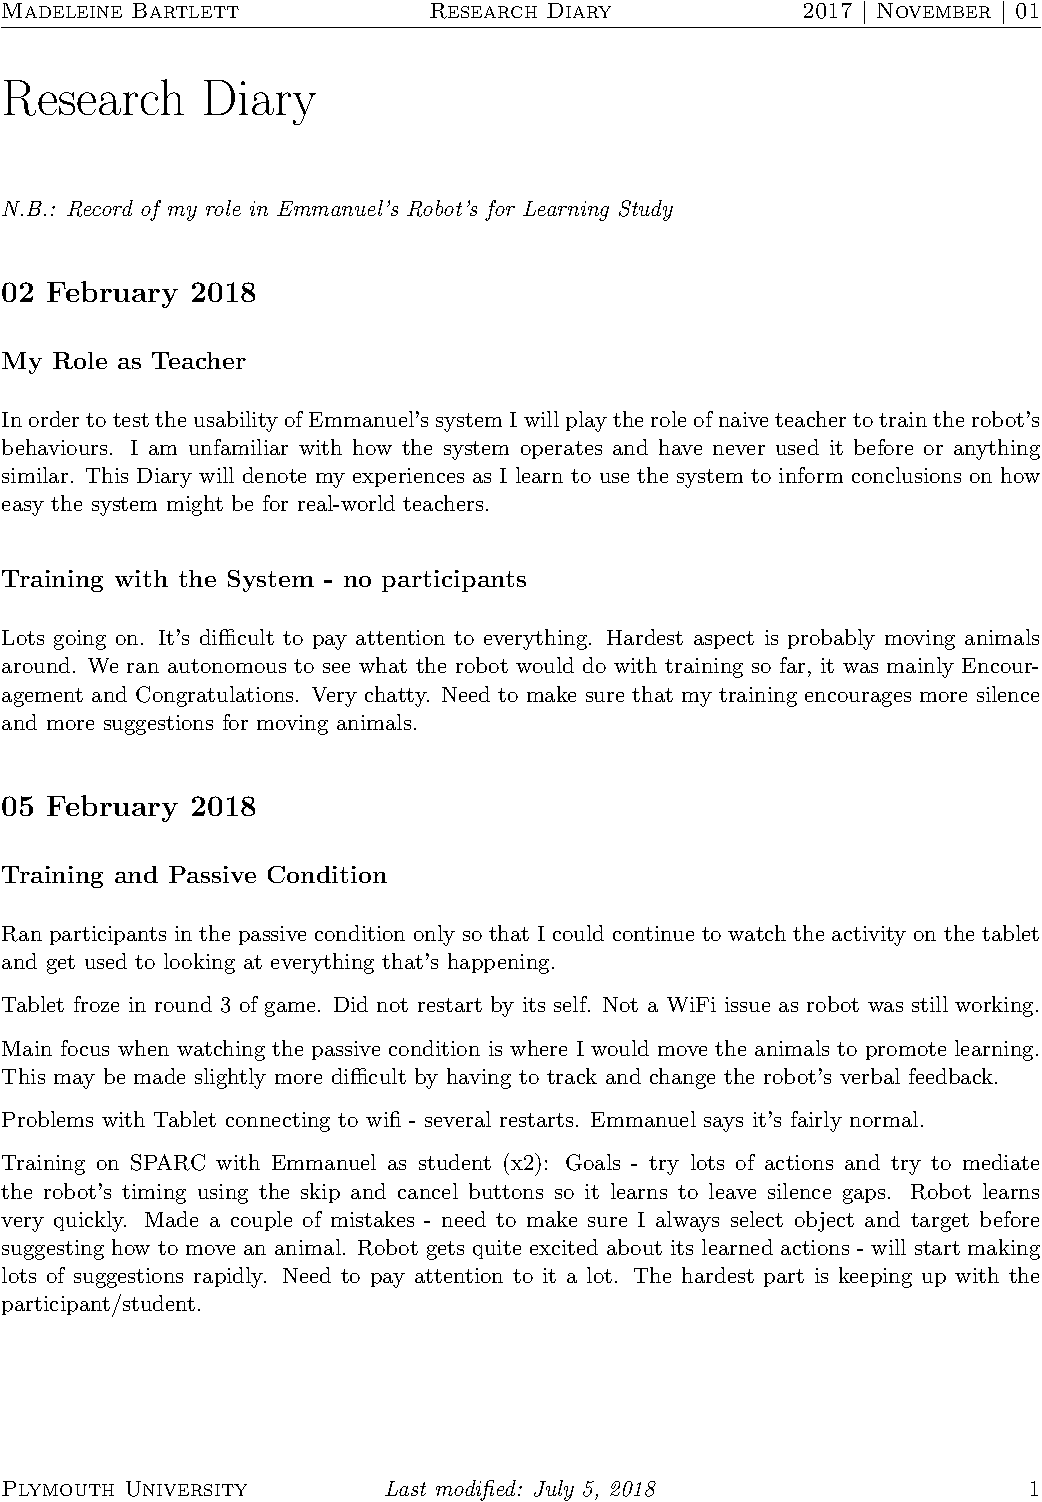
\includepdf[pages=1-14,pagecommand={},linktodoc=true]{appendices/research-diary.pdf}
\foreachpage{appendices/research-diary.pdf}{%
	\newpage   
	\begingroup 
	\centering
	\includegraphics[
	page=\value{imagepage},
	width=\textwidth,  
	height=\textheight,
	keepaspectratio,
	]{appendices/research-diary.pdf}%
	\newpage
	\endgroup
}
\end{appendices}
\cleartooddpage

%%%%%%%%%%%%%%%%%%%%%%%%%%%%%%%%%%%%%%%%%%%%%%%%%%%%%%%%%%%%%%%%%%%%%%%%%%%%
{\setstretch{1.0}
\bibliographystyle{prelim/apa-good}
\bibpunct[ ]{(}{)}{;}{a}{}{,}
\phantomsection
\addcontentsline{toc}{chapter}{Bibliography}
\bibliography{ThesisBib}
\cleartooddpage
}

%%%%%%%%%%%%%%%%%%%%%%%%%%%%%%%%%%%%%%%%%%%%%%%%%%%%%%%%%%%%%%%%%%%%%%%%%%%%

\end{document}
